
\documentclass[11pt]{article}
\usepackage{geometry}                % See geometry.pdf to learn the layout options. There are lots.
\geometry{letterpaper} 
\usepackage[parfill]{parskip}    % Activate to begin paragraphs with an empty line rather than an indent
\usepackage{graphicx}
\usepackage{amsmath,amssymb}
\usepackage{actuarialsymbol}
\usepackage{listings}
\usepackage{subcaption}
\usepackage{amssymb, amsmath}
\usepackage{epstopdf}
\usepackage{wrapfig}
\usepackage{algorithm}
\usepackage{algpseudocode}
\usepackage{color} % For custom colors
\usepackage{listings} % For code listings
\usepackage{xcolor} % Enhanced color support

\usepackage{a4wide,fancyhdr,tikz}
\pagestyle{fancy}
\fancyhf{}
\fancyhead[L]{MT7072 Assignment 1}
\fancyhead[R]{Andreas Hansson \& Oscar Johansson}
\fancyfoot[C]{\thepage}

% Define custom colors
\definecolor{codegreen}{rgb}{0,0.6,0}
\definecolor{codegray}{rgb}{0.5,0.5,0.5}
\definecolor{codepurple}{rgb}{0.58,0,0.82}
\definecolor{backcolour}{rgb}{0.95,0.95,0.92}

% Setup the lstlisting environment
\lstset{language=R,
    backgroundcolor=\color{backcolour},   
    keywordstyle=\color{magenta},
    numberstyle=\tiny\color{codegray},
    stringstyle=\color{codepurple},
    basicstyle=\footnotesize\ttfamily, % or \small or \footnotesize etc.
    basicstyle=\scriptsize\ttfamily, % Smaller font size'
    breakatwhitespace=false,         
    breaklines=true,                 
    captionpos=b,                    
    keepspaces=true,                 
    numbers=left,                    
    numbersep=5pt,                  
    showspaces=false,                
    showstringspaces=false,
    showtabs=false,                  
    tabsize=2
}

\DeclareGraphicsRule{.tif}{png}{.png}{`convert #1 `dirname #1`/`basename #1 .tif`.png}

\title{Report II - MT7027 Risk Models and Reserving in Non-Life Insurance}
\author{Andreas Hansson, Oscar Johansson}
\date{\today}
                                    % Activate to display a given date or no date

\usepackage[parfill]{parskip}

\begin{document}
\maketitle
\section*{Objectives}
This project sees to simulate a claim portfolio consisting of 2 insurance branches.
The aim is to gain an understanding how insurance claims are distributed and how, through simulations, one can estimate distributions of  claim costs.
The second part of the project is to understand reinsurance and see how reinsurance affects the total claim cost based on individual cases in an XL-cover, and on a portfolio level using SL-covers.

The data provided is a 10 year old portfolio claim history containing 2 branches of insurances.
We will use this data to estimate the distribution of claims, and simulate the claim cost for a single year of this portfolio based on the data.

The project is divided into a short mathematical background explaining the necessary theory behind the work, and then the results will be presented according to the assignment.
We will not explain the individual assignments but refer to the project description for these.
Finally we provide the code that has generated the output for these results.

\section*{Mathematical Background}

\subsection*{Claim-Severity Model}
In this project we will model our claim cost as 2 different processes, a claim arrival process and a claim severity model.
In doing so we assume that the claim arrival is indipendent from the claim cost.
Modeling these separately comes with practical applications, as the arrival process and claim severity often follow parametric distributions, often the poisson and gamma respectively.
One could dismiss these distribution and use other technology to predict claims, or use a joint distribution like the Tweedie distribution. 
Using the Tweedie, we would assume a poisson-gamma compount distribution, which may or may not be suitable.


\subsection*{Kolmogorov-Smirnov}
In analysing the distributions observe, and understand the best model fit, we use the Kolmogorov–Smirnov test to compare the quantile to quantile plots.
In using the Kolmogorov–Smirnov (K-S) test, we calculate the maximum distance between the empirical distribution function of the sample and the cumulative distribution function of the reference distribution. 
This non-parametric test provides a critical value for the significance level chosen, allowing us to determine whether the observed sample distribution significantly differs from the theoretical distribution. 
This approach is non-parametric and used as much of the distribution analysis we do is based on qq-plots, which is what the Kolmogorov–Smirnov test measures.

\subsection*{Overdispersion}
An other property which will be discussed through this assignment is overdispersion, and namely the quasi-poisson distribution.
Overdispersion is a phenomenon observed when the variance in the data is higher than the mean. This condition often indicates that the data do not follow a Poisson distribution, which assumes equality between the mean and variance. 
In such cases, the quasi-Poisson distribution becomes a valuable tool for analysis. 
Unlike the traditional Poisson model, the quasi-Poisson allows for the variance to be a linear function of the mean, effectively adjusting for the overdispersion by introducing a dispersion parameter.  
An alternative would be the negative binomial, but as will later be seen, the quasi-poisson distribution showed to be a better fit for the data.

\section*{Results}

\subsection*{Estimating the claim intensity.}
In analysing the claim intensity we study how the intensity has varied through the years, and if there is a time-dependency of the claim intensity.
Studying the arrival times through a year we observe that the intensity is much lower during the summer periods of the year, see figure \ref{a1:intensity}. 
The reason for this may be many, but likely we are working with a product having strong seasonalities, and in conjustion with the amount and the claim amounts, it seems this could be 2 branches of motor insurances.

\begin{figure}[h!]
    \centering
    \begin{subfigure}[t]{0.5\textwidth}
        \centering
        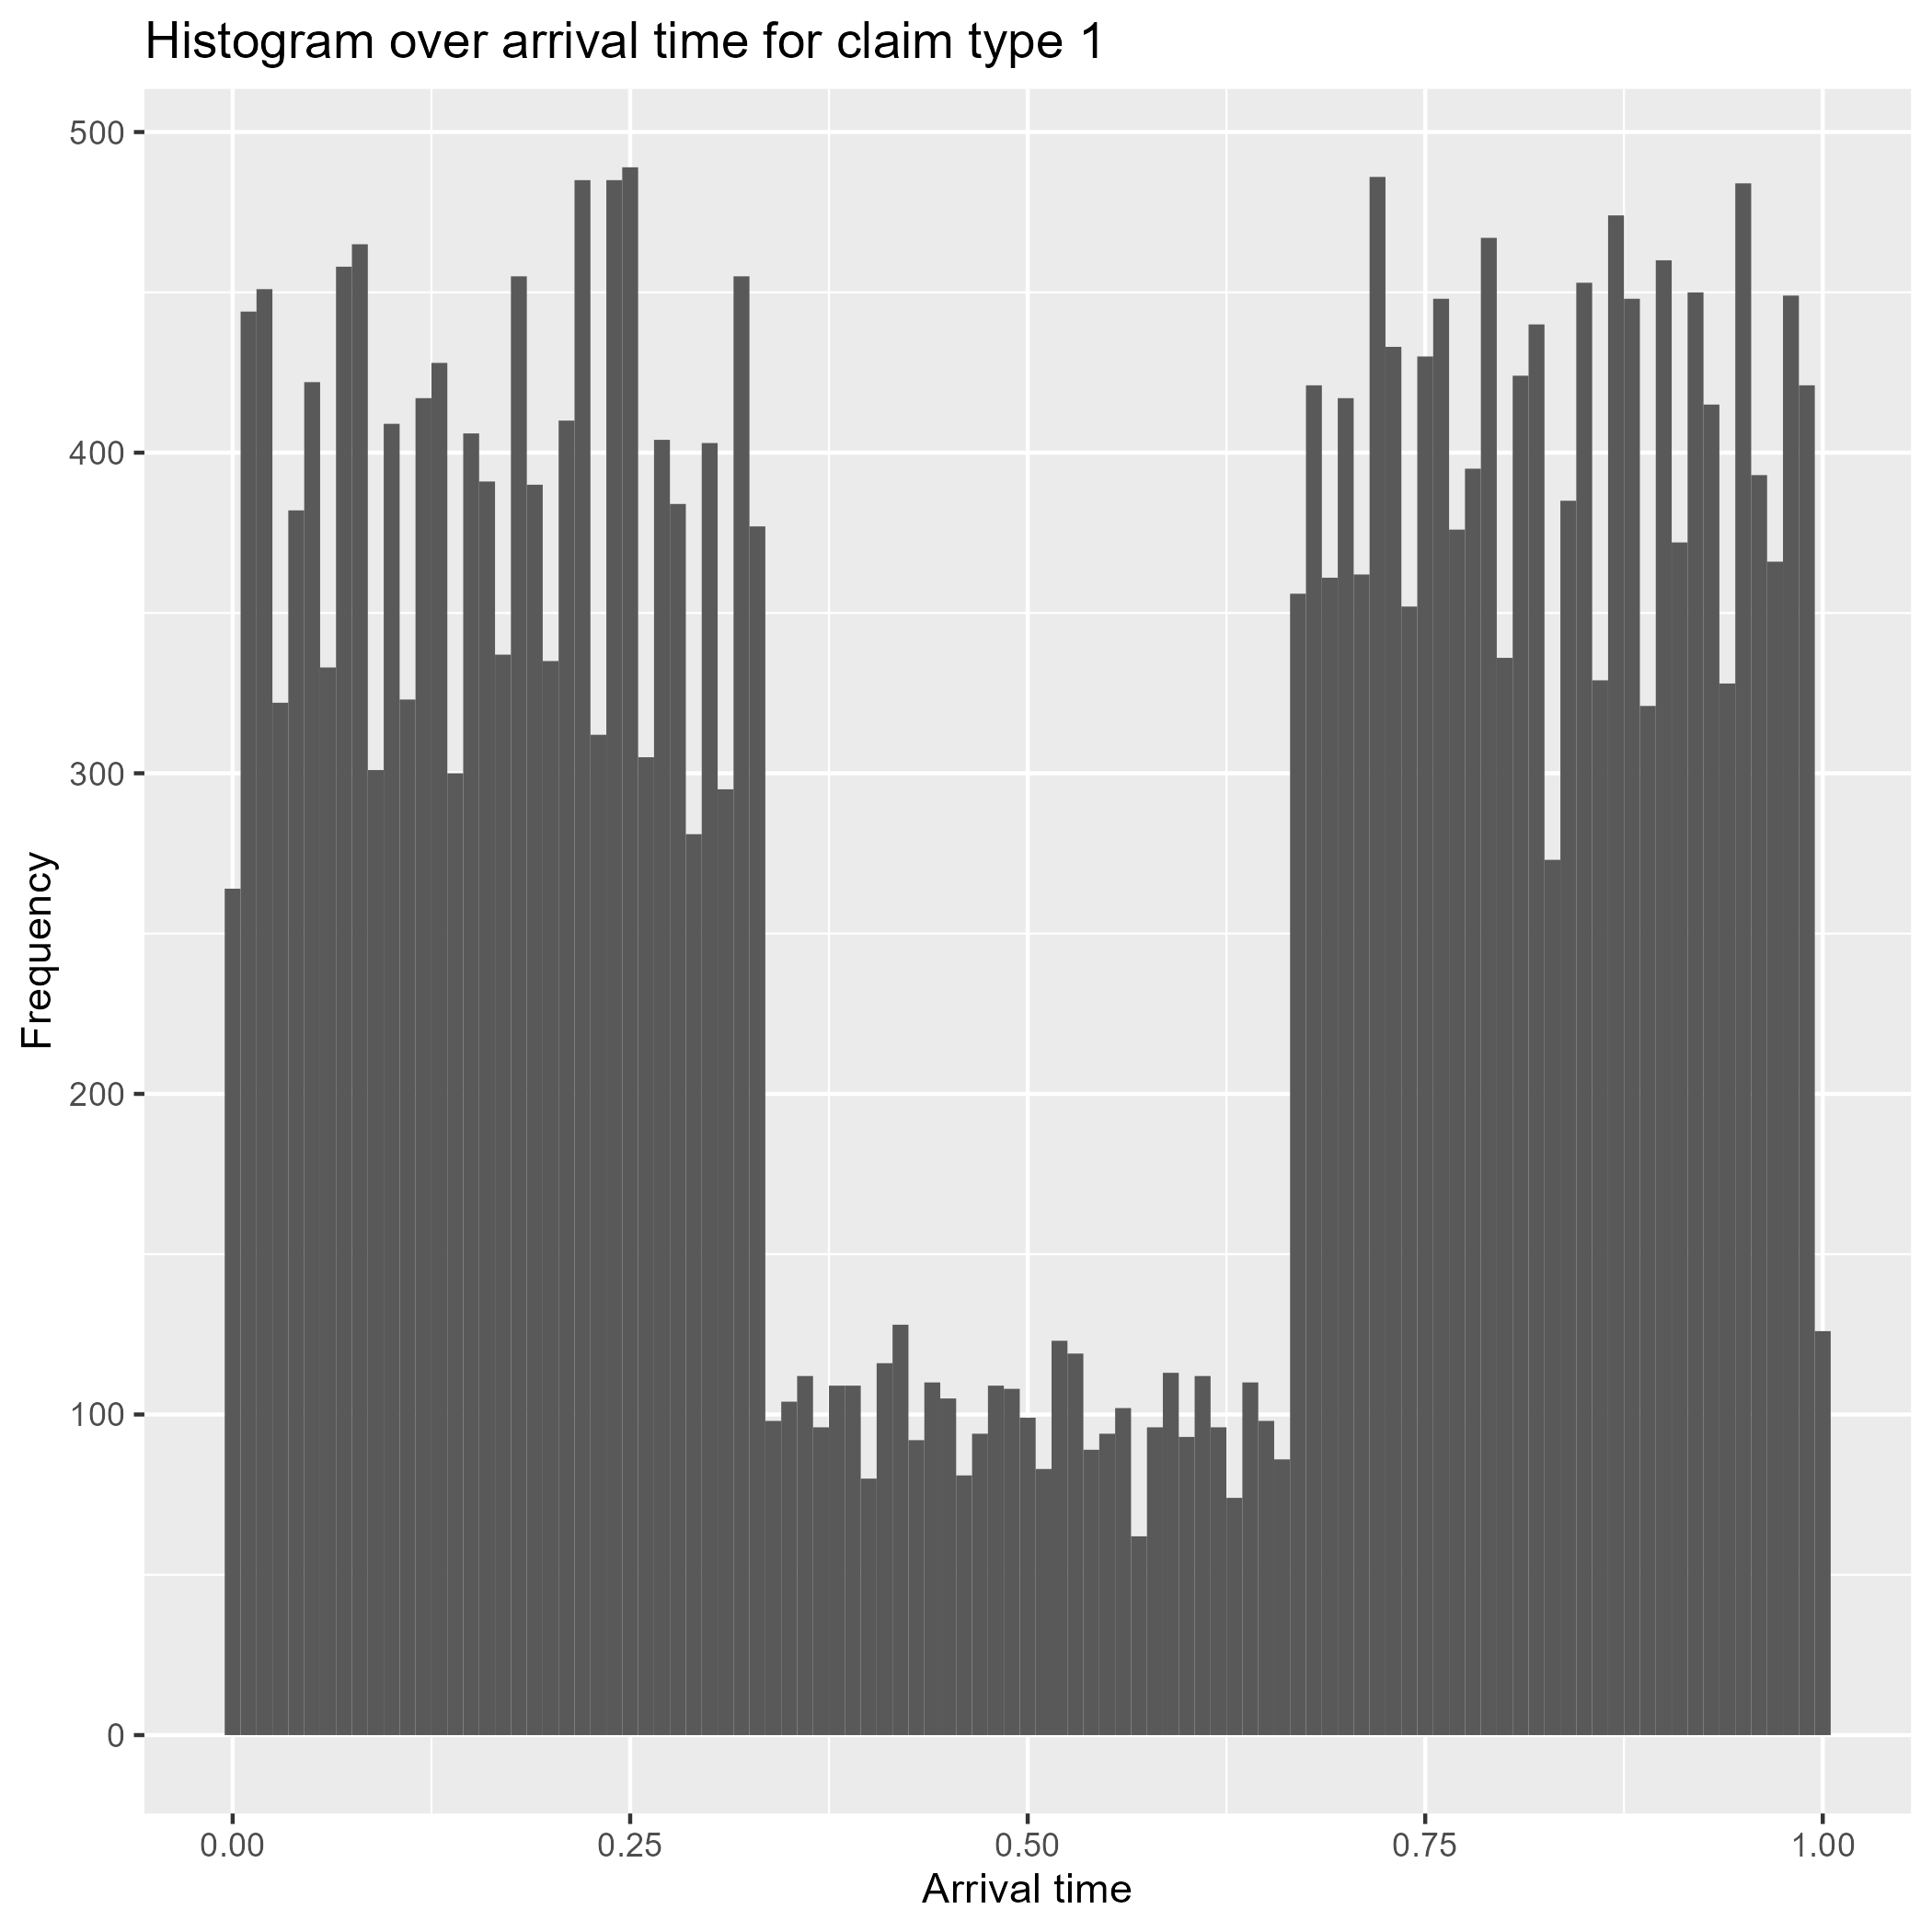
\includegraphics[width=0.8\textwidth]{plots/claim_type1/histogram_arrivaltime_s.png}
        \caption{Branch 1.}
    \end{subfigure}%
    ~ 
    \begin{subfigure}[t]{0.5\textwidth}
        \centering
        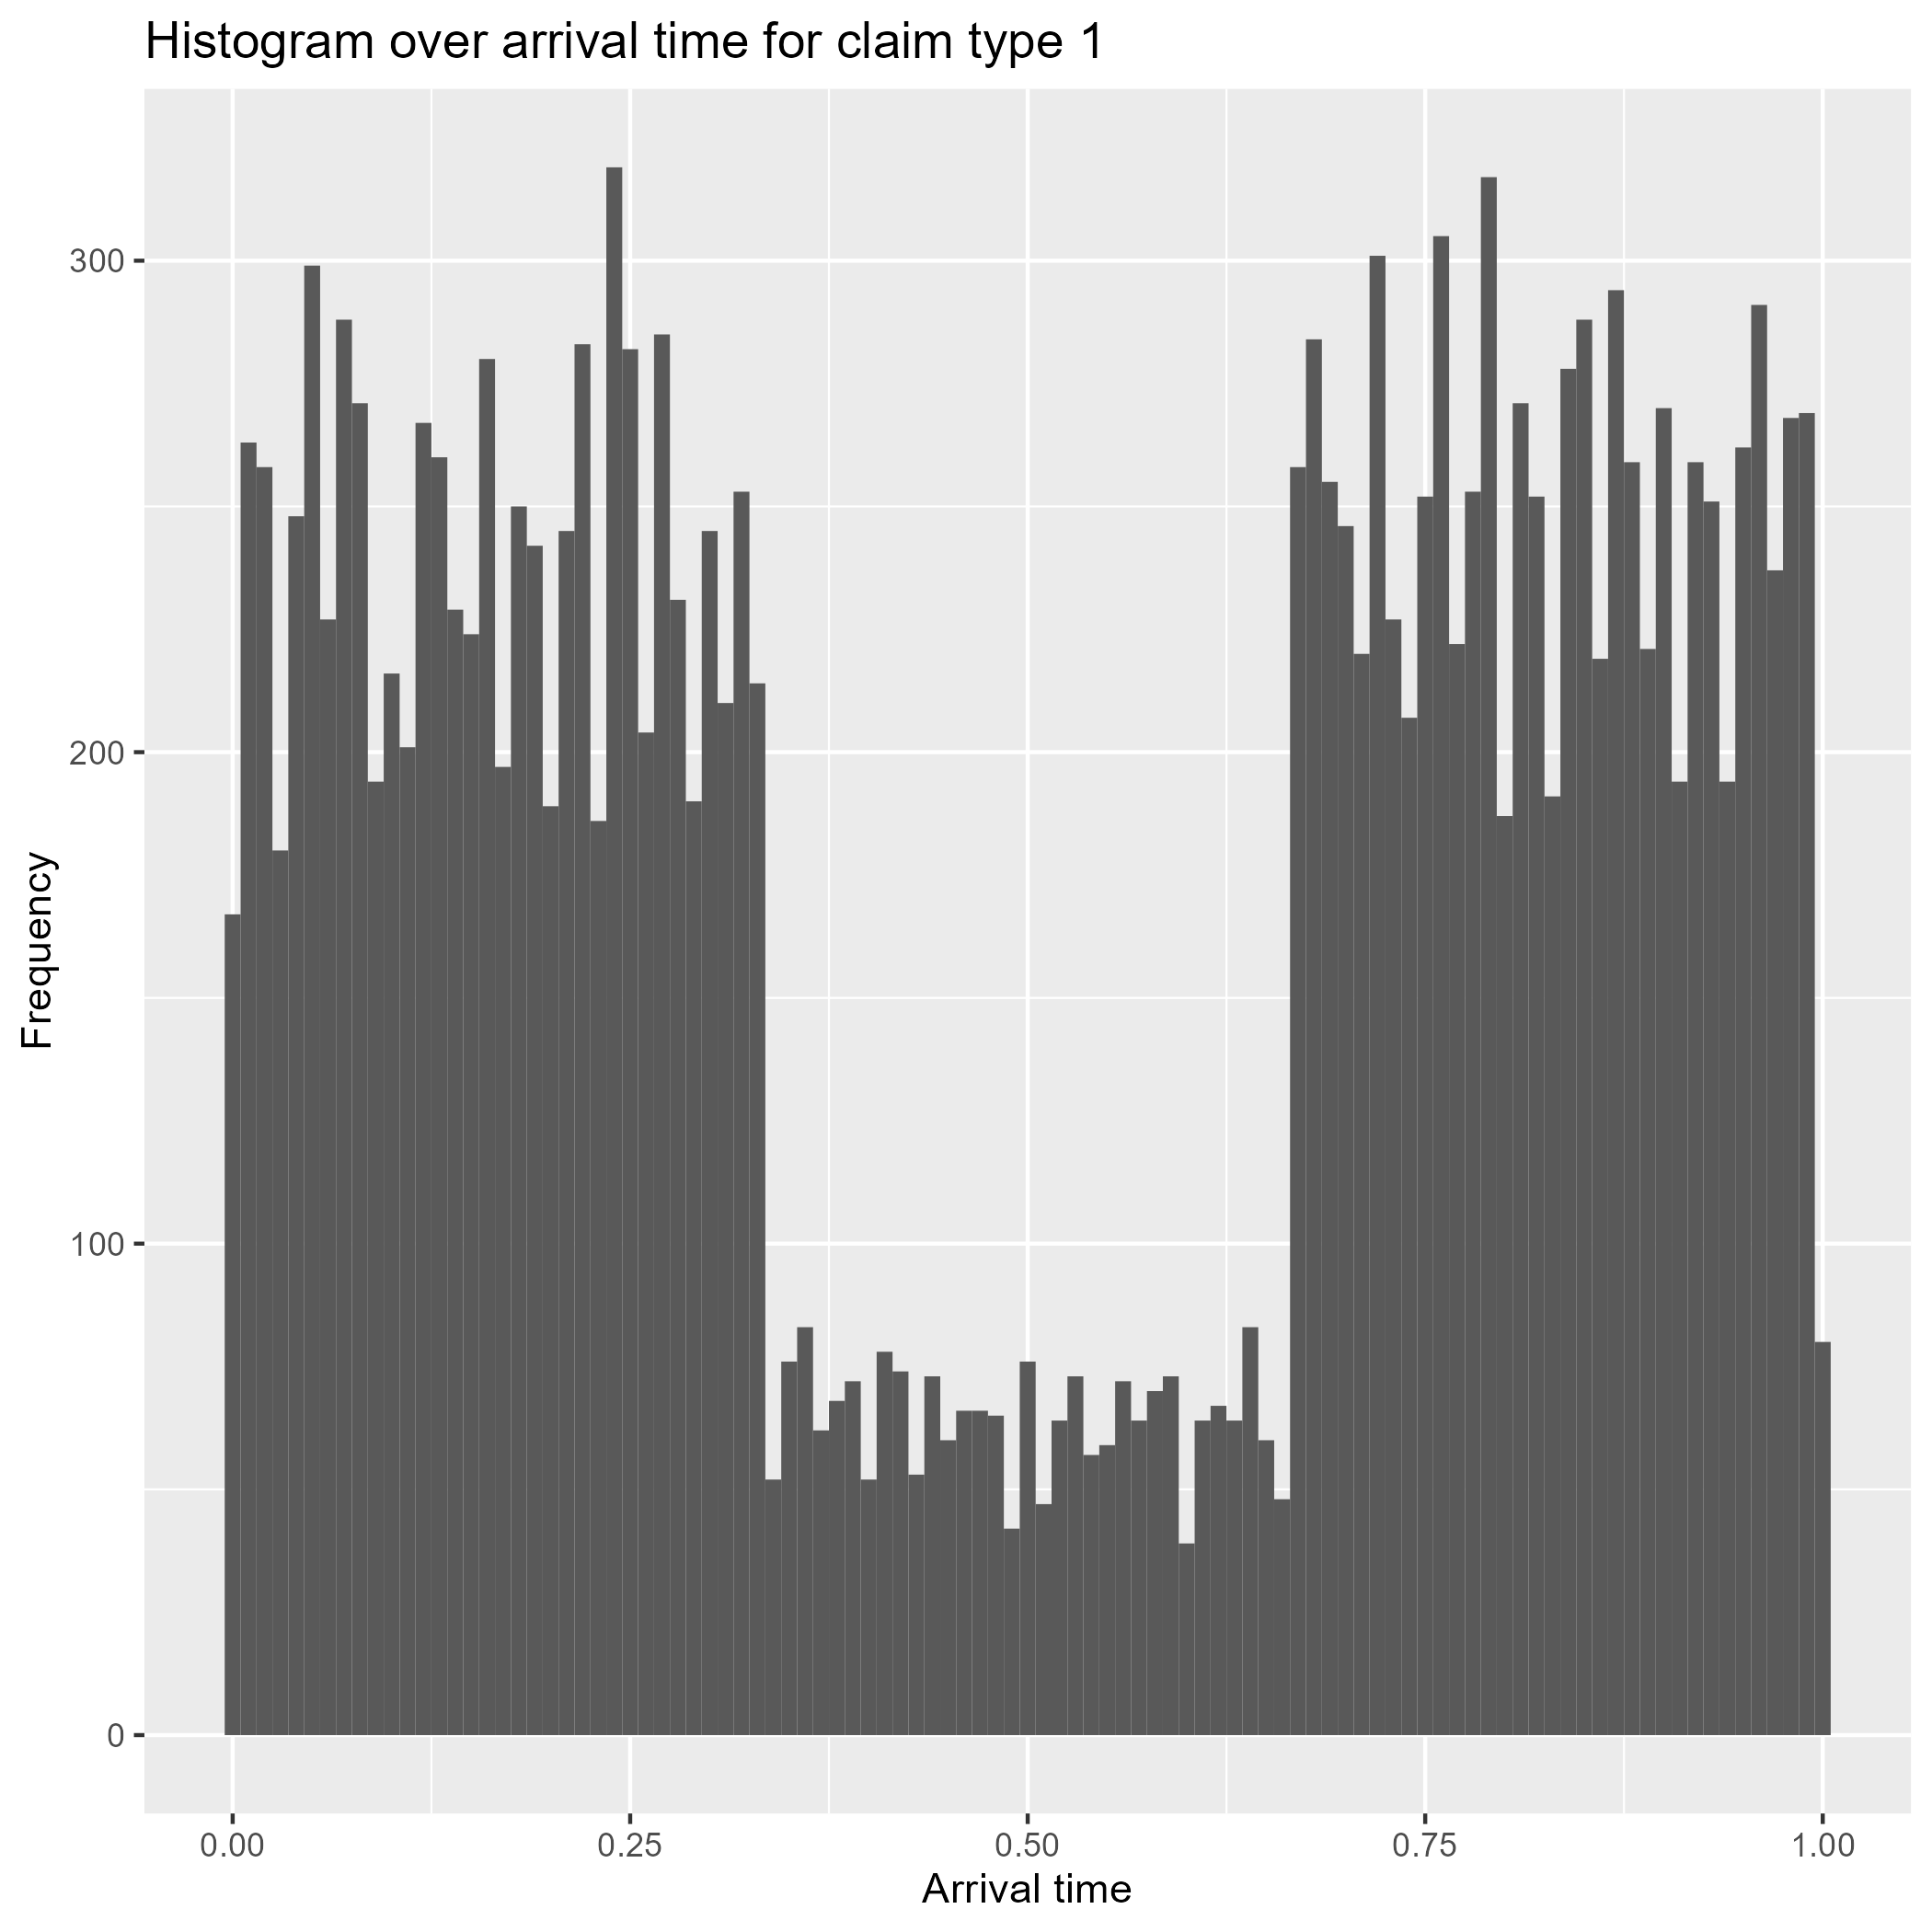
\includegraphics[width=0.8\textwidth]{plots/claim_type2/histogram_arrivaltime_s.png}
        \caption{Branch 2.}
    \end{subfigure}
    \caption{Claim intensity with time of year $s$.}
    \label{a1:intensity}
\end{figure}

The seasonality was the only significant effect we saw for the intensity when studying the branches individually.
Additionally we studied
\begin{itemize}
    \item The arrival time as a dependence of of time $t$.
    \item The arrival time as a function of the claim size (small or large).
    \item The arrival time as a function of the in year time $s$
\end{itemize}

All these tests can be found in the code, and no significant effect was found when modeling the arrival data as a Poisson GLM regression to various polynomial degree and covariance.
We assume here that the data follows a non-homogeneous Poisson process with independence between days and no auto-correlation between our claims.

We also studied other arrival distributions like the gamma and the quasi-poisson distribution but only foundy significant effect if the period was during the summer period, defined as 
\begin{equation}
    I_{summer} = \begin{cases}
      1 & \text{if } s\in{[\frac{4}{12},\frac{8}{12}]}\\
      0 & \text{otherwise}
    \end{cases}  
    \label{eq:summer}
\end{equation}

where $s$ is the time in the year, with $0$ being the first of january and $1$ last of December. 
This is not the final model fit for the arrival process, as we later will study the covariate between the 2 insurance branches, but on a branch by branch basis, this was we found as significant.

In the end we observed that the arrival process likely arrives from a over-dispersed Poisson distribution, but we will go into that later when modeling the covariance between the branches.
Aggregating the data and counting the amount of claims per day, seen in figure \ref{a1:histogram}, we observe that the difference between the summer period and non-summer period with a quite high frequency of claims and that there seem to be some other covariant for branch 1, and also branch 2.

\begin{figure}[h!]
    \begin{subfigure}{.49\textwidth}
        \centering
        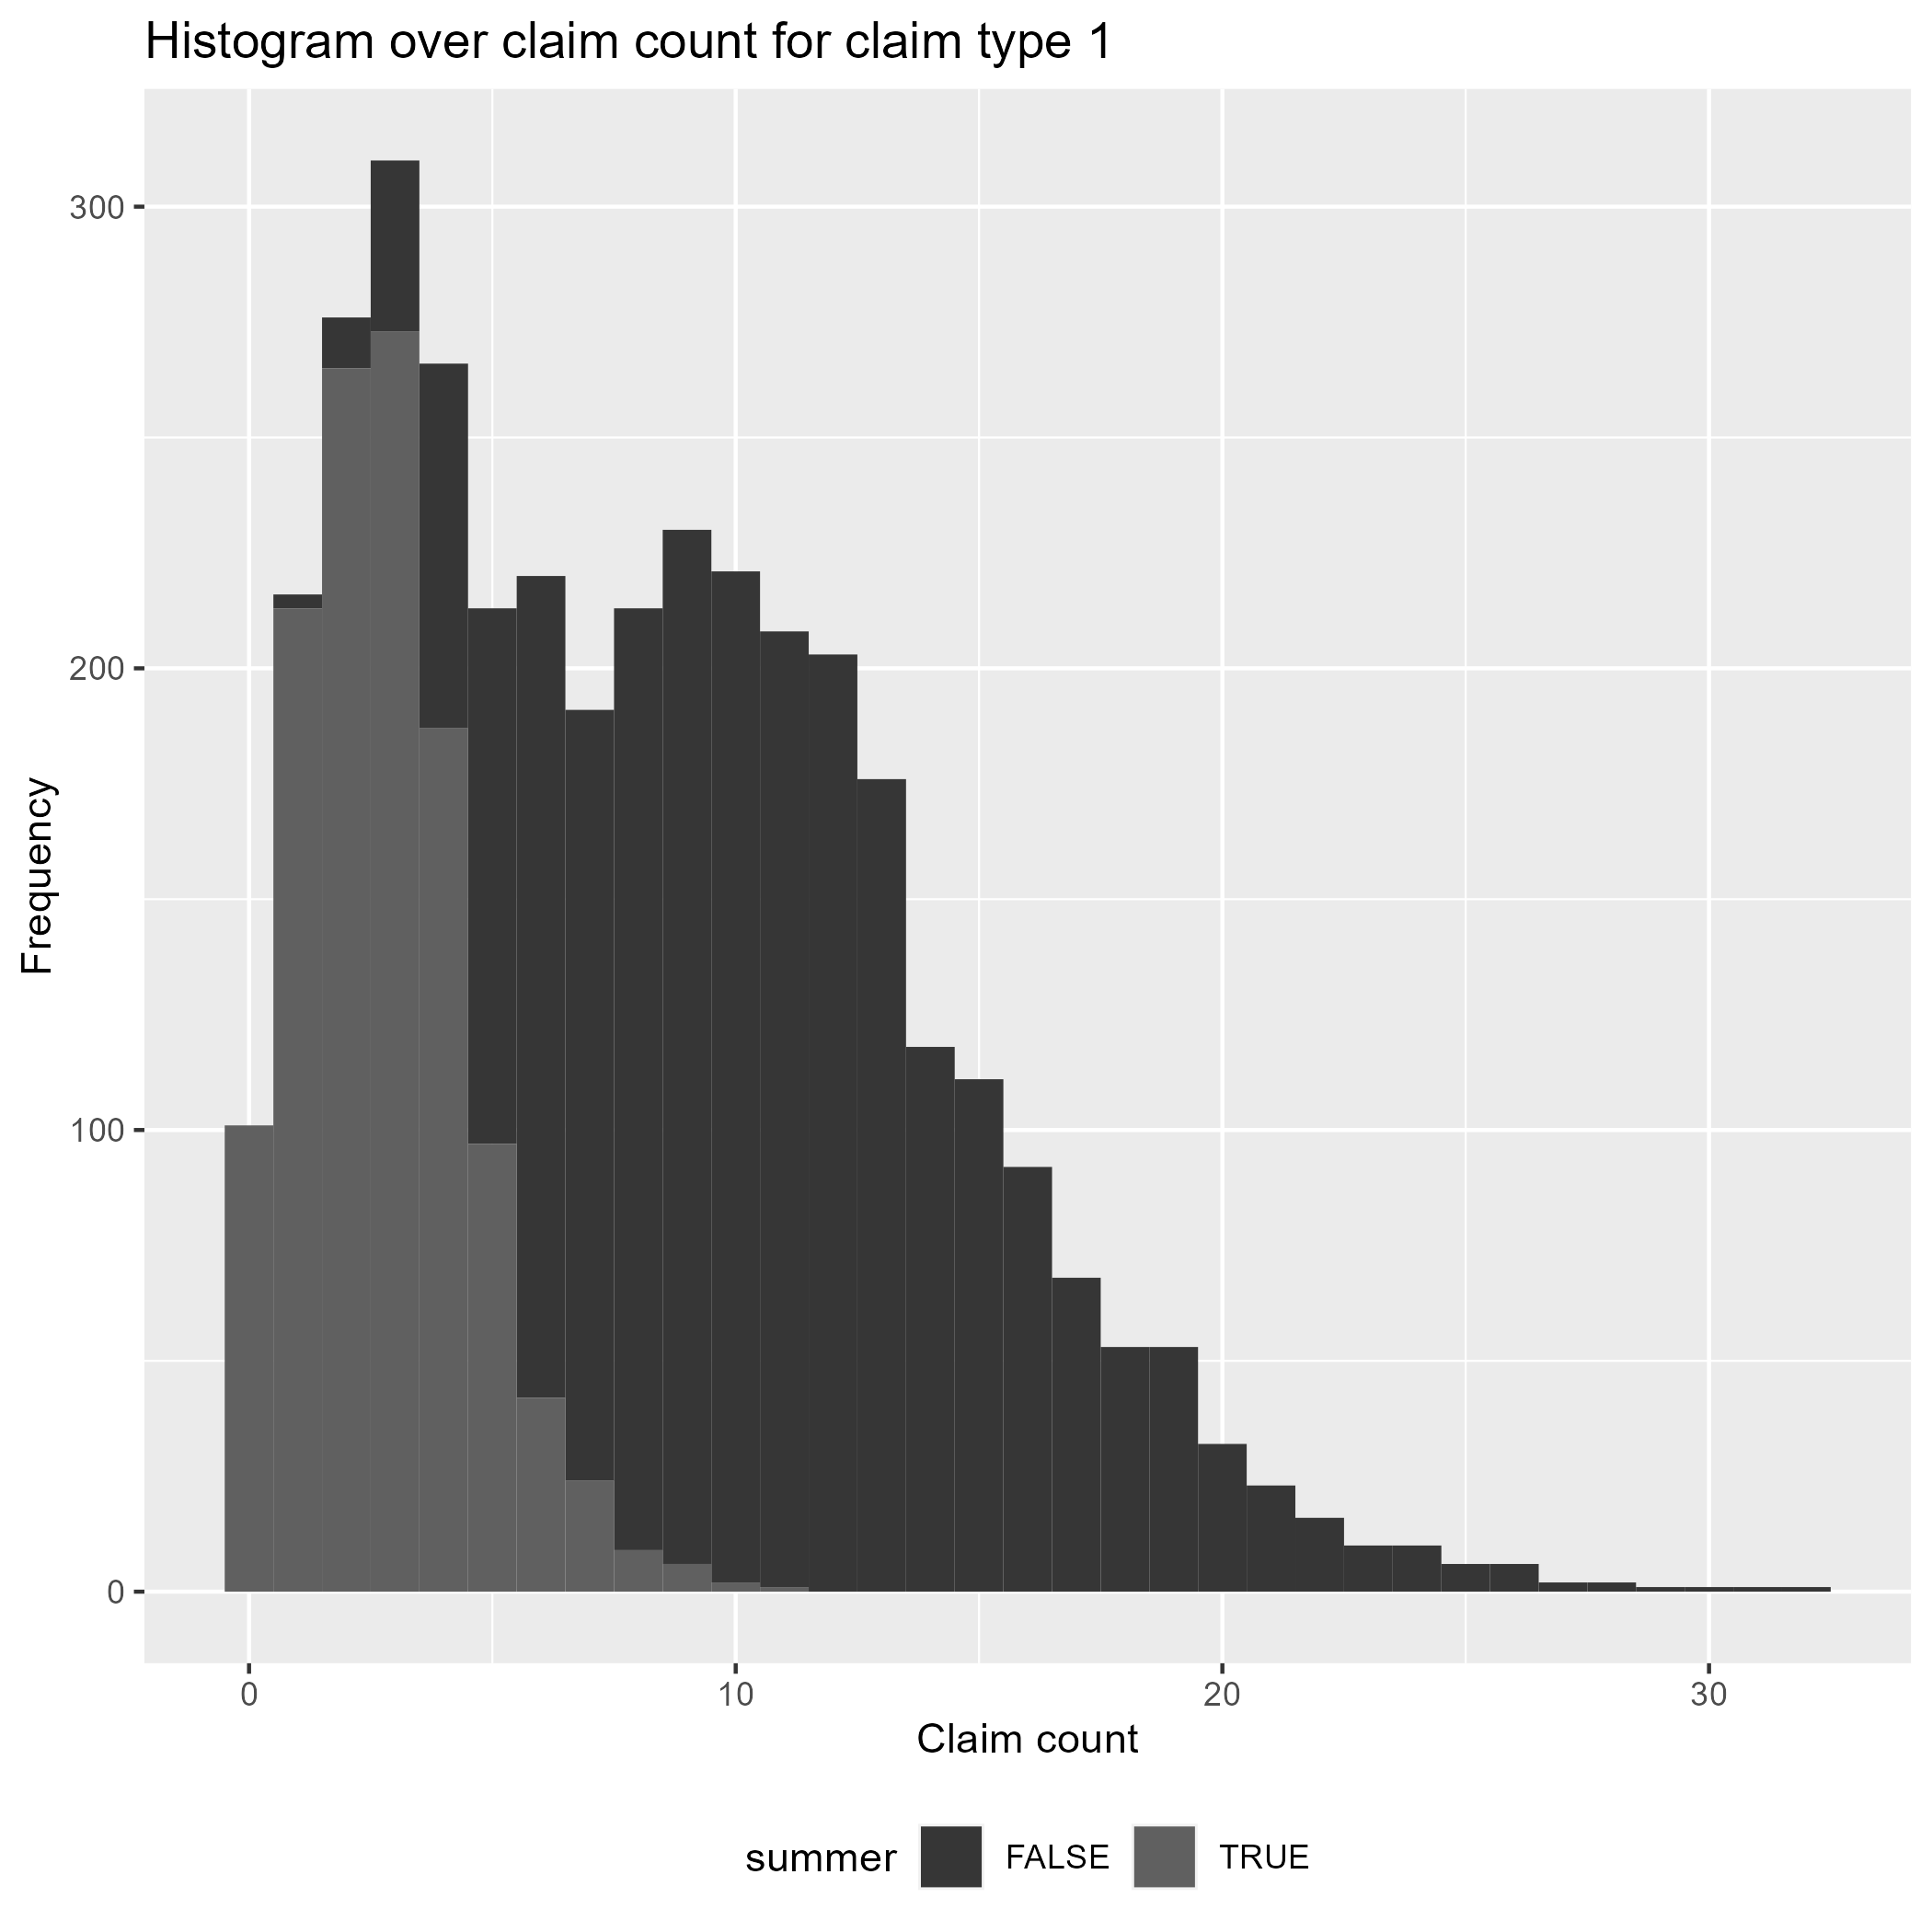
\includegraphics[width=.9\linewidth]{plots/covariance/histogram_claim_count1.png}
        \caption{Branch 1.}
        \label{a3:claimamount}
    \end{subfigure}
    \begin{subfigure}{.49\textwidth}
        \centering
        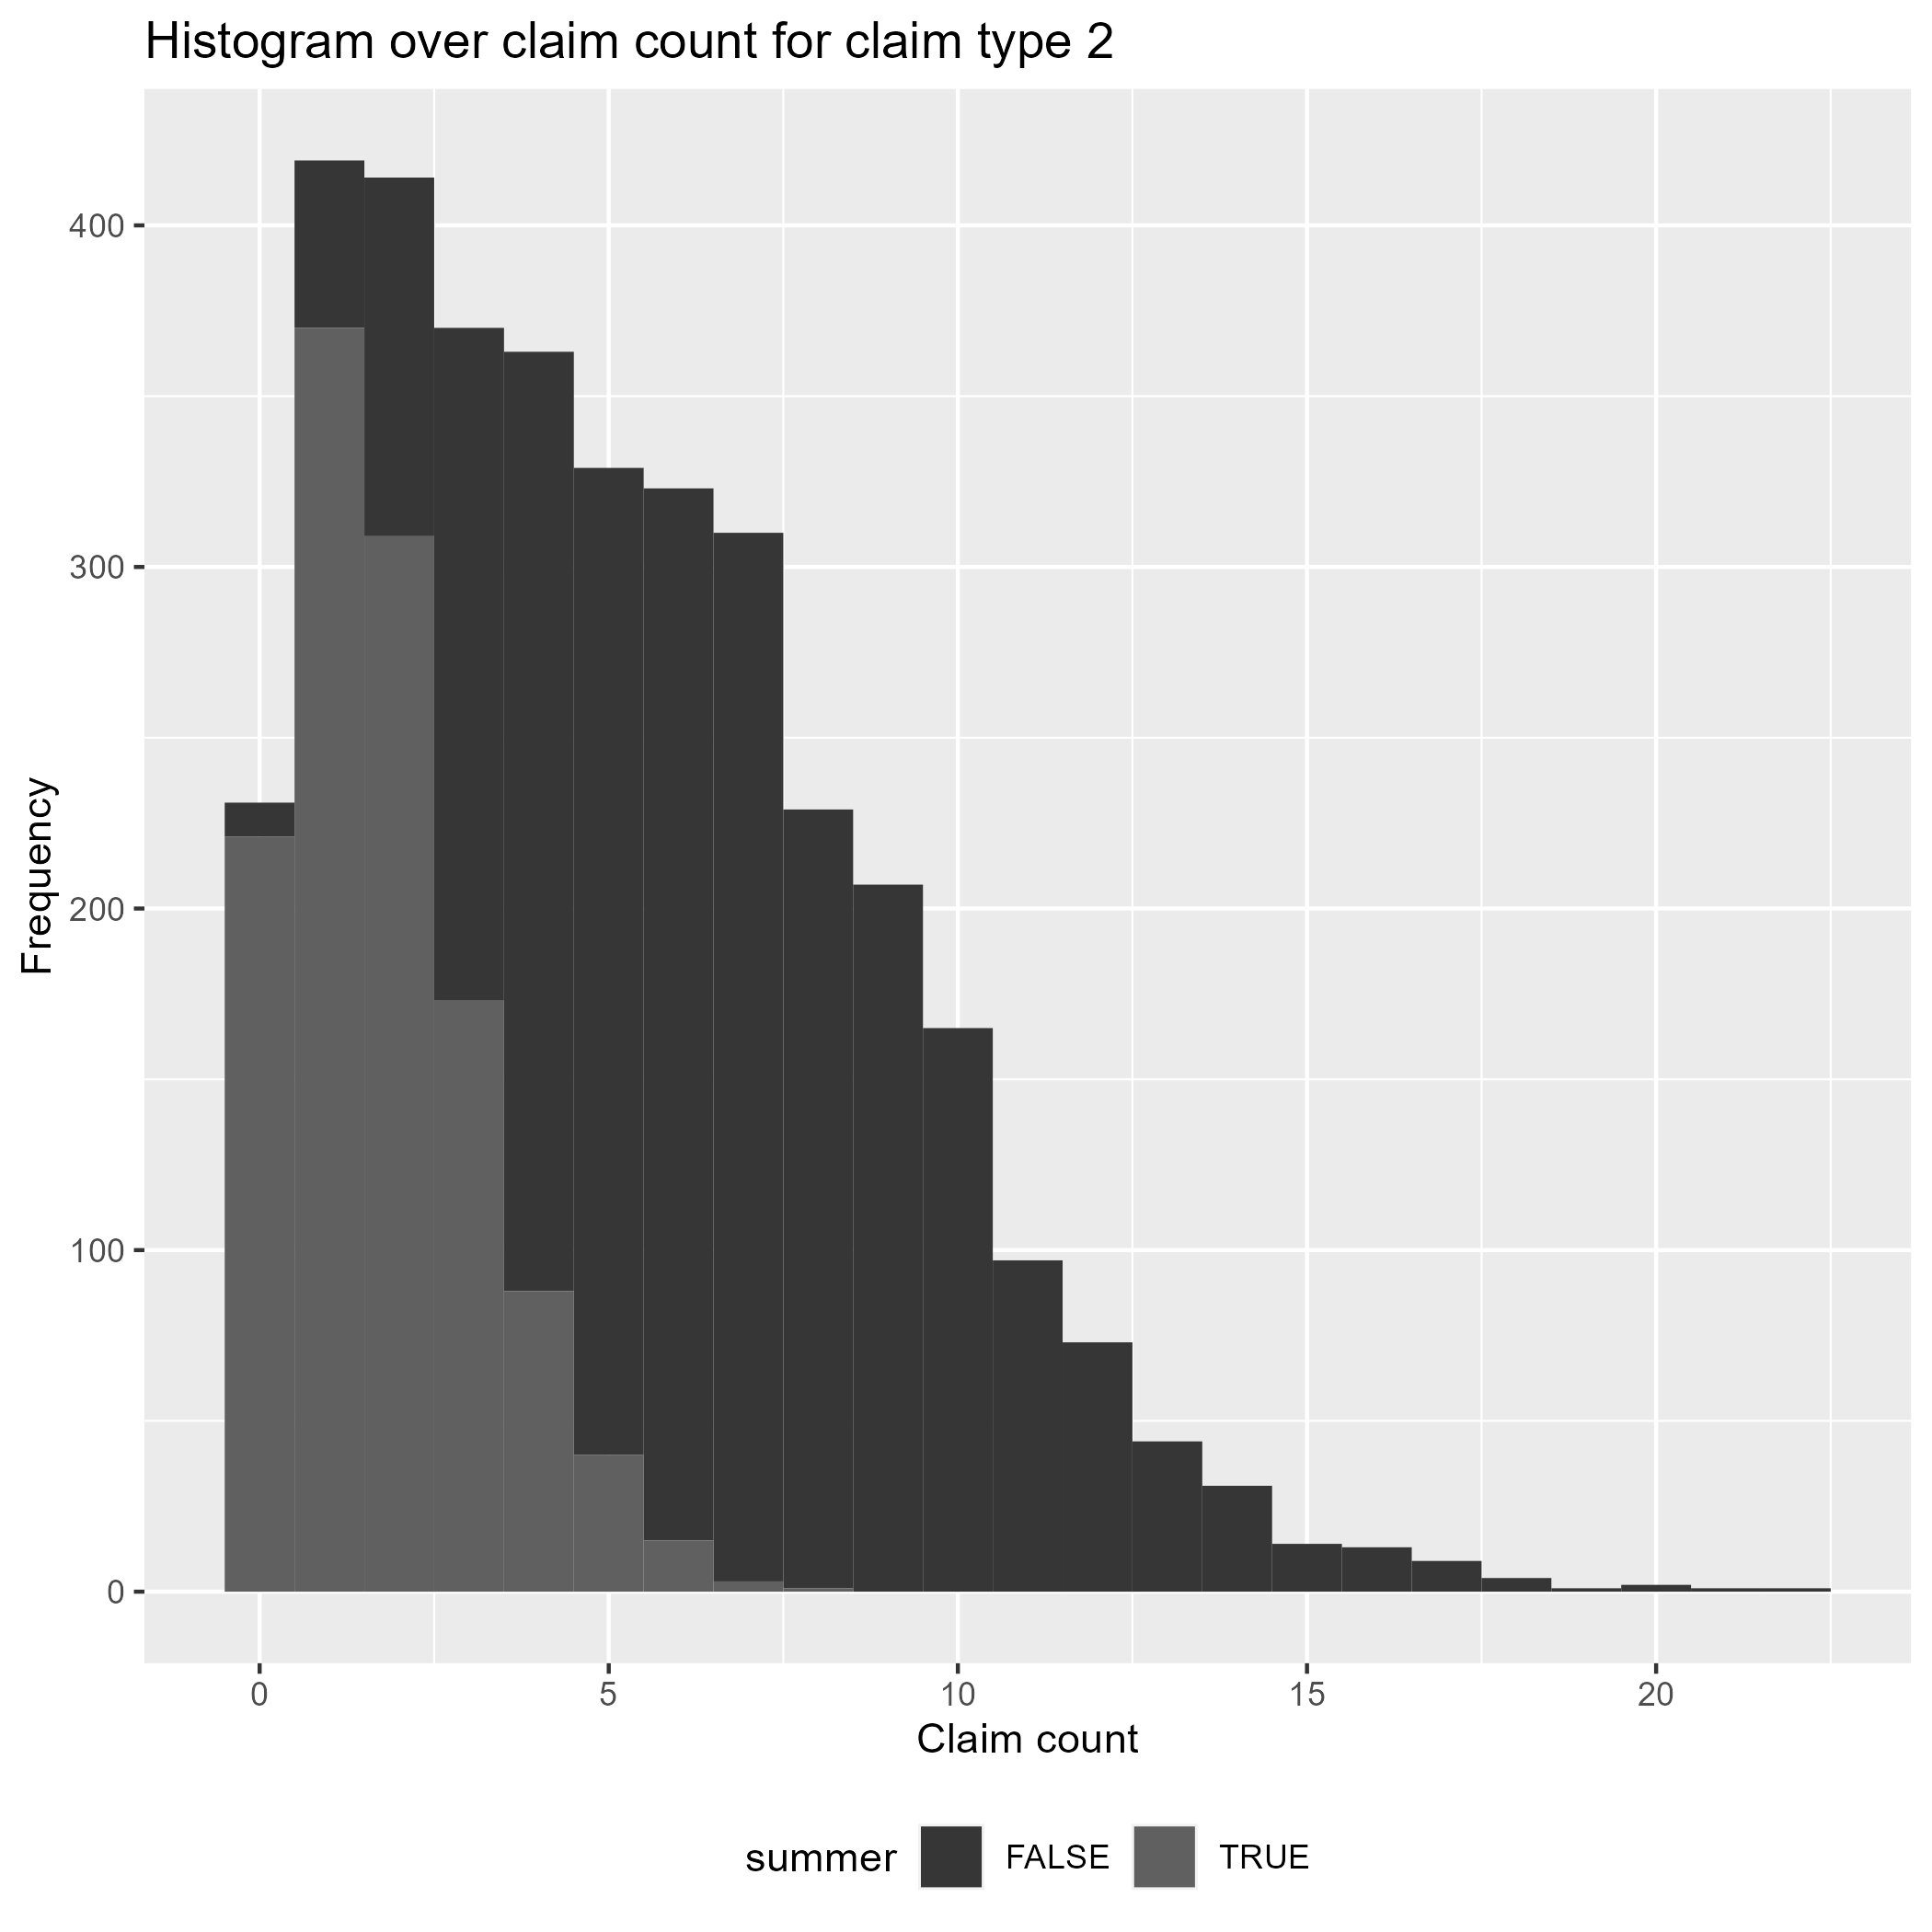
\includegraphics[width=.9\linewidth]{plots/covariance/histogram_claim_count2.png}
        \caption{Branch 2.}
        \label{a1:histogram}
    \end{subfigure}
\end{figure}

\subsection*{Estimating the claim severity.}
Analysing the size of the claims we quickly understand from plotting the distributions, see figure \ref{a2:severity}, that there seem to be a mixture distribution of claims.
It seem quite easy to distinguish into large claims and small claims.
As such we studied the severity in higher granularity by dividing them into small or large based on thresholds $10^5$ for branch 1, and $10^6$ for branch 2.

Do also observe that the branch 2 has much higher severity and larger variance compared to branch 1. 
To further the speculation of what type of insurance product this is, it could be that branch 1 are motor damages meanwhile branch 2 are motor injuries, often being subject for much larger claims than the cars they where driving.

\begin{figure*}[t!]
    \centering
    \begin{subfigure}[t]{0.5\textwidth}
        \centering
        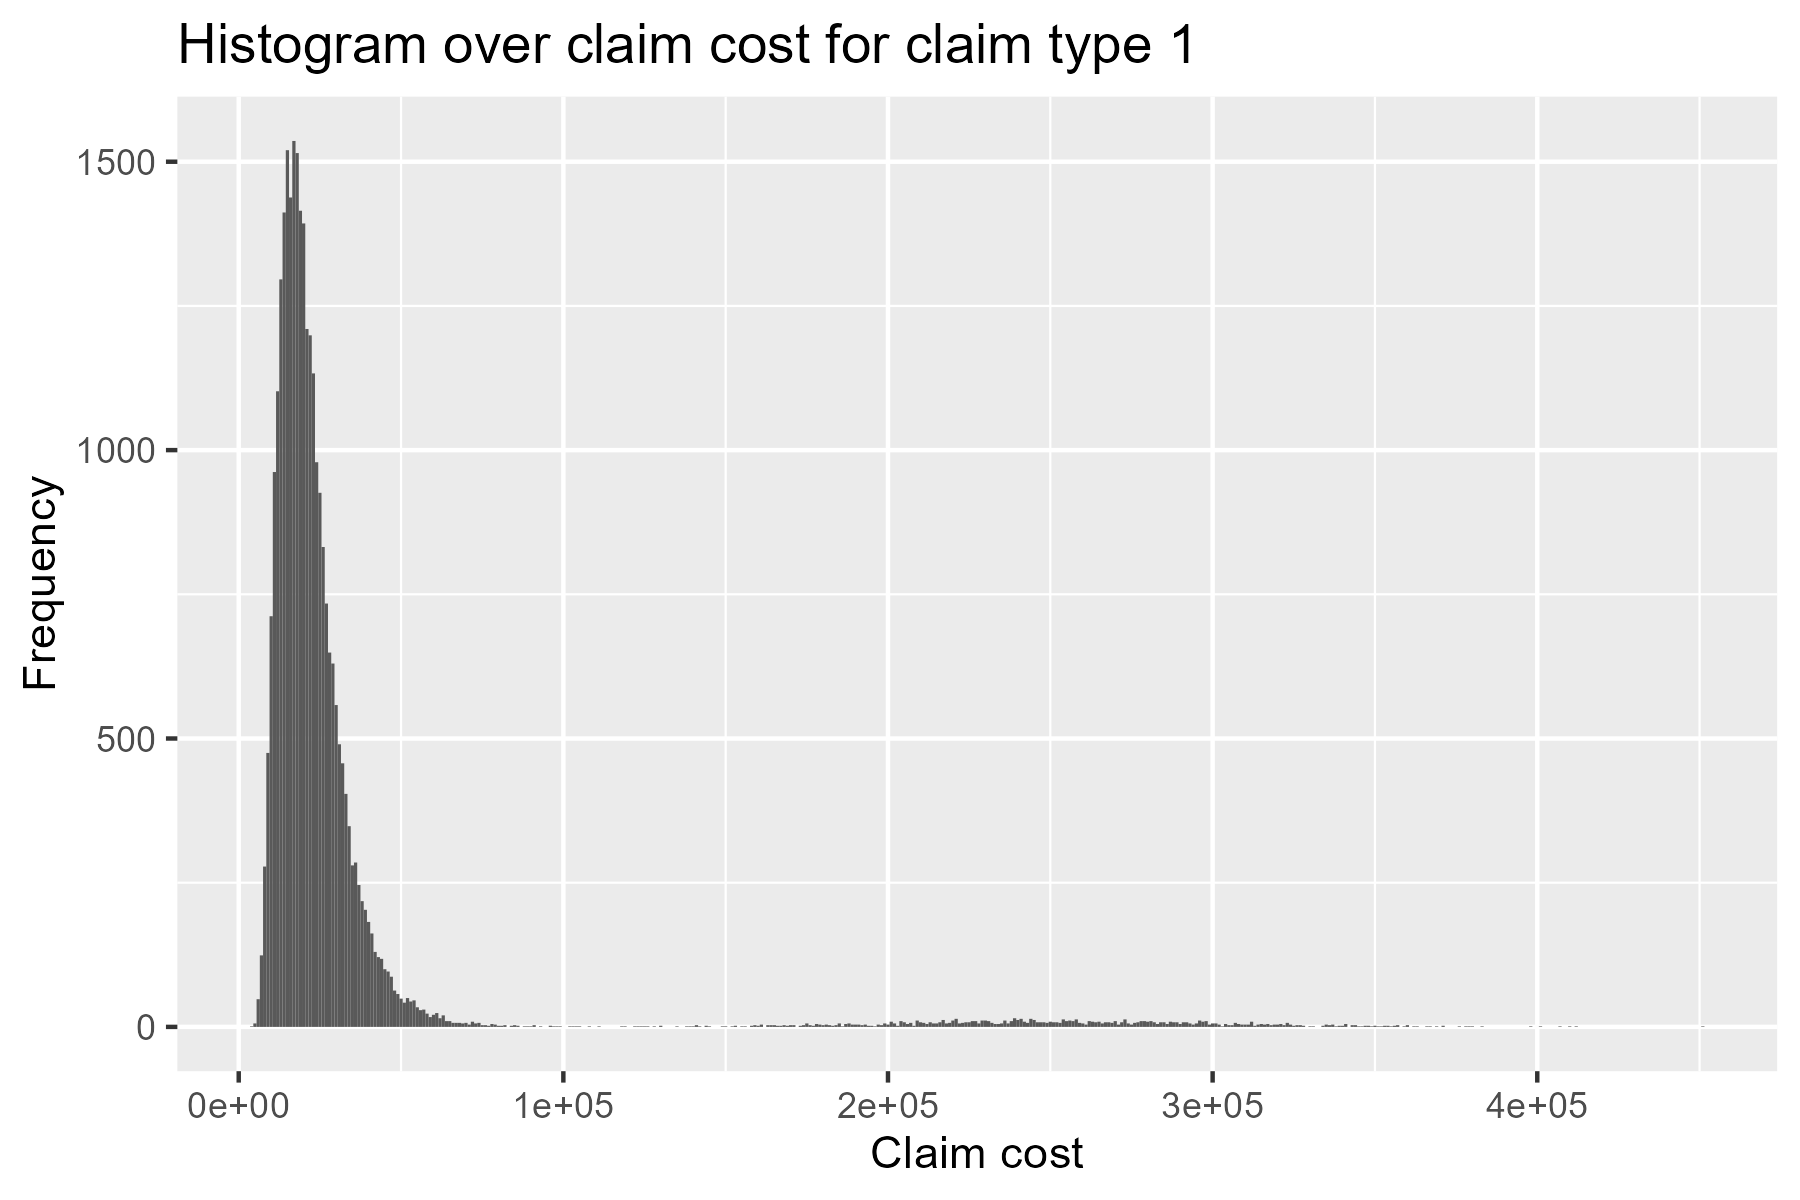
\includegraphics[width=0.95\textwidth]{plots/claim_type1/histogram_claimcost.png}
        \caption{Claim severity in branch 1.}
    \end{subfigure}%
    ~ 
    \begin{subfigure}[t]{0.5\textwidth}
        \centering
        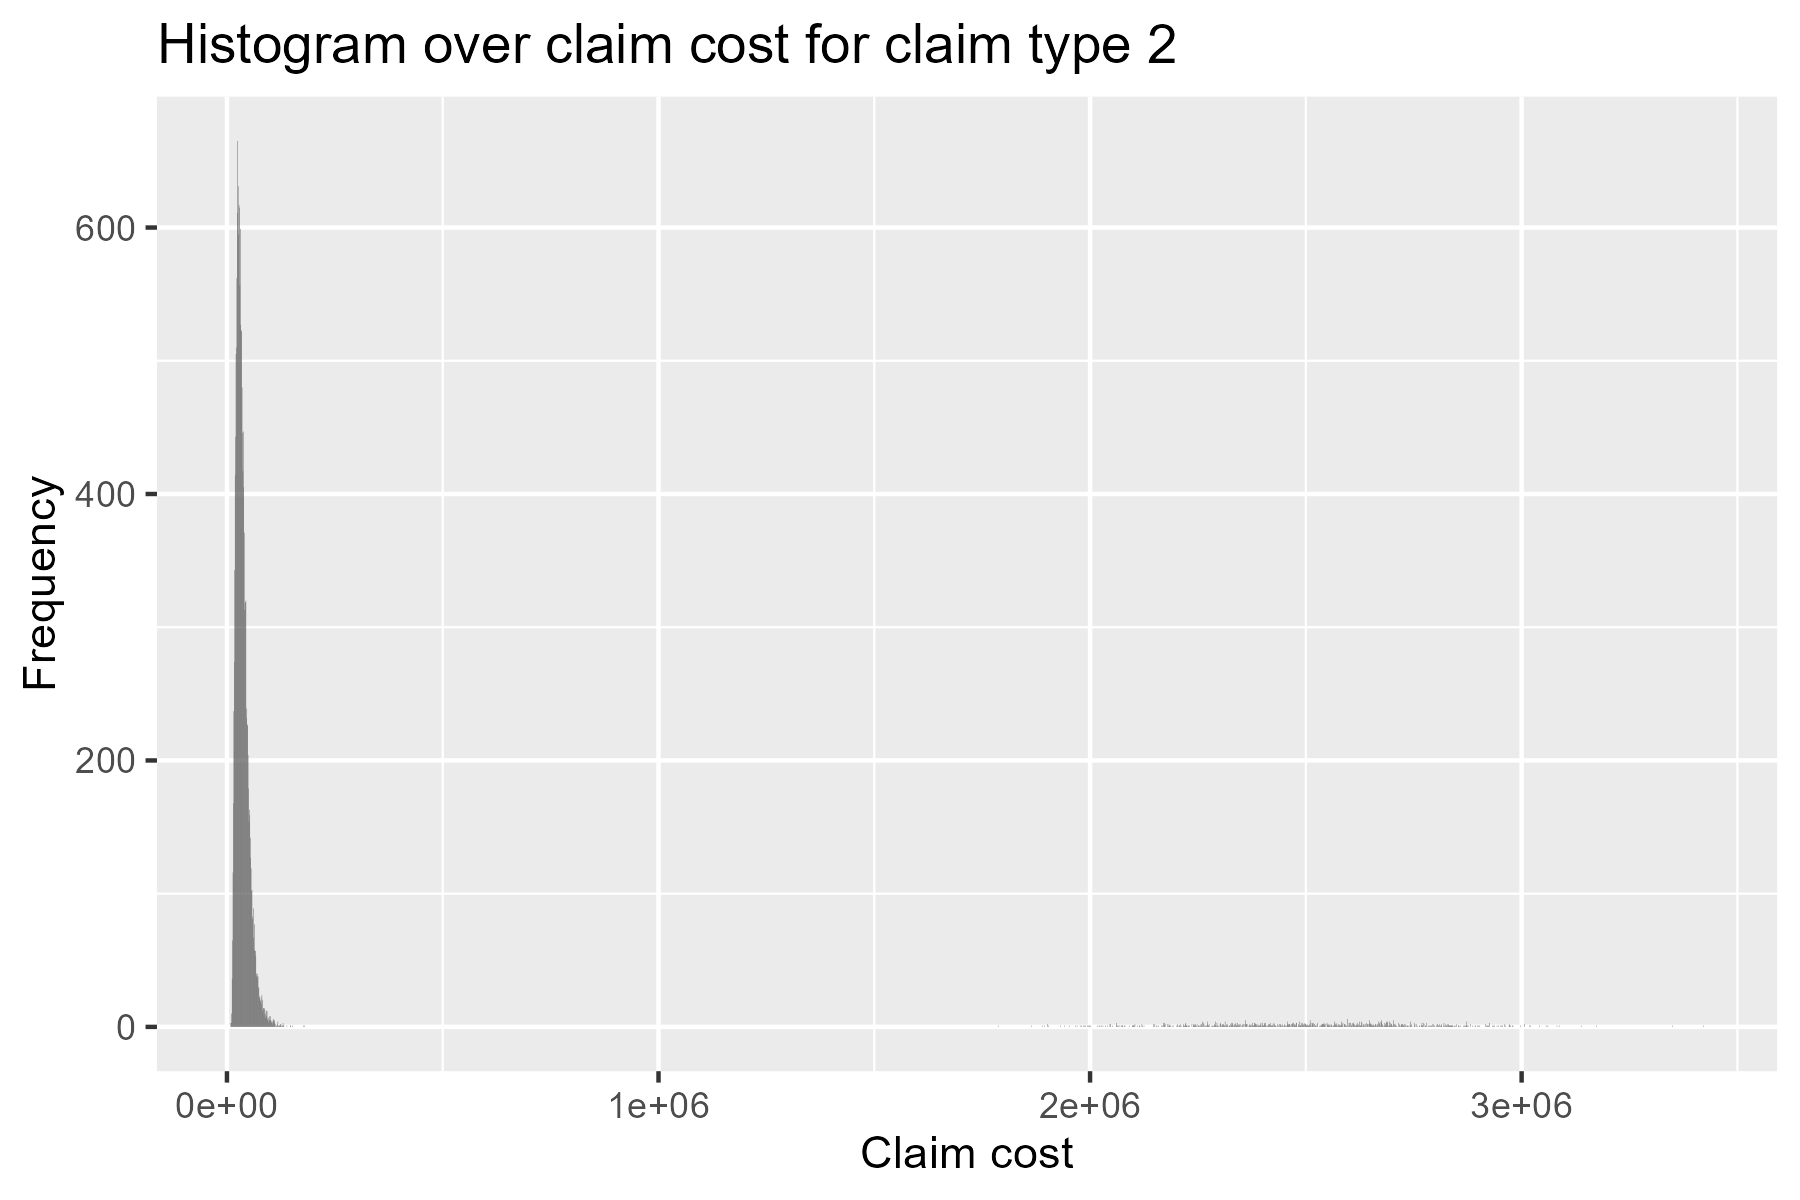
\includegraphics[width=0.95\textwidth]{plots/claim_type2/histogram_claimcost_2.png}
        \caption{Claim severity in branch 2.}
    \end{subfigure}
    \caption{Claim Severity in the 2 branches.}
    \label{a2:severity}
\end{figure*}

Studying the large claims, seen in figure \ref{a2:largeqq}, we observe that these claims following a normal distribution.
This was validated through a Kolmogorov–Smirnov test and from studying covariance of time such as time $t$, time in year $s$ and summer indicator as defined in \ref{eq:summer}, no significant covariance where found using standard linear regression.


\begin{figure}[!h]
\centering
\begin{subfigure}{.49\textwidth}
    \begin{subfigure}{.5\textwidth}
      \centering
      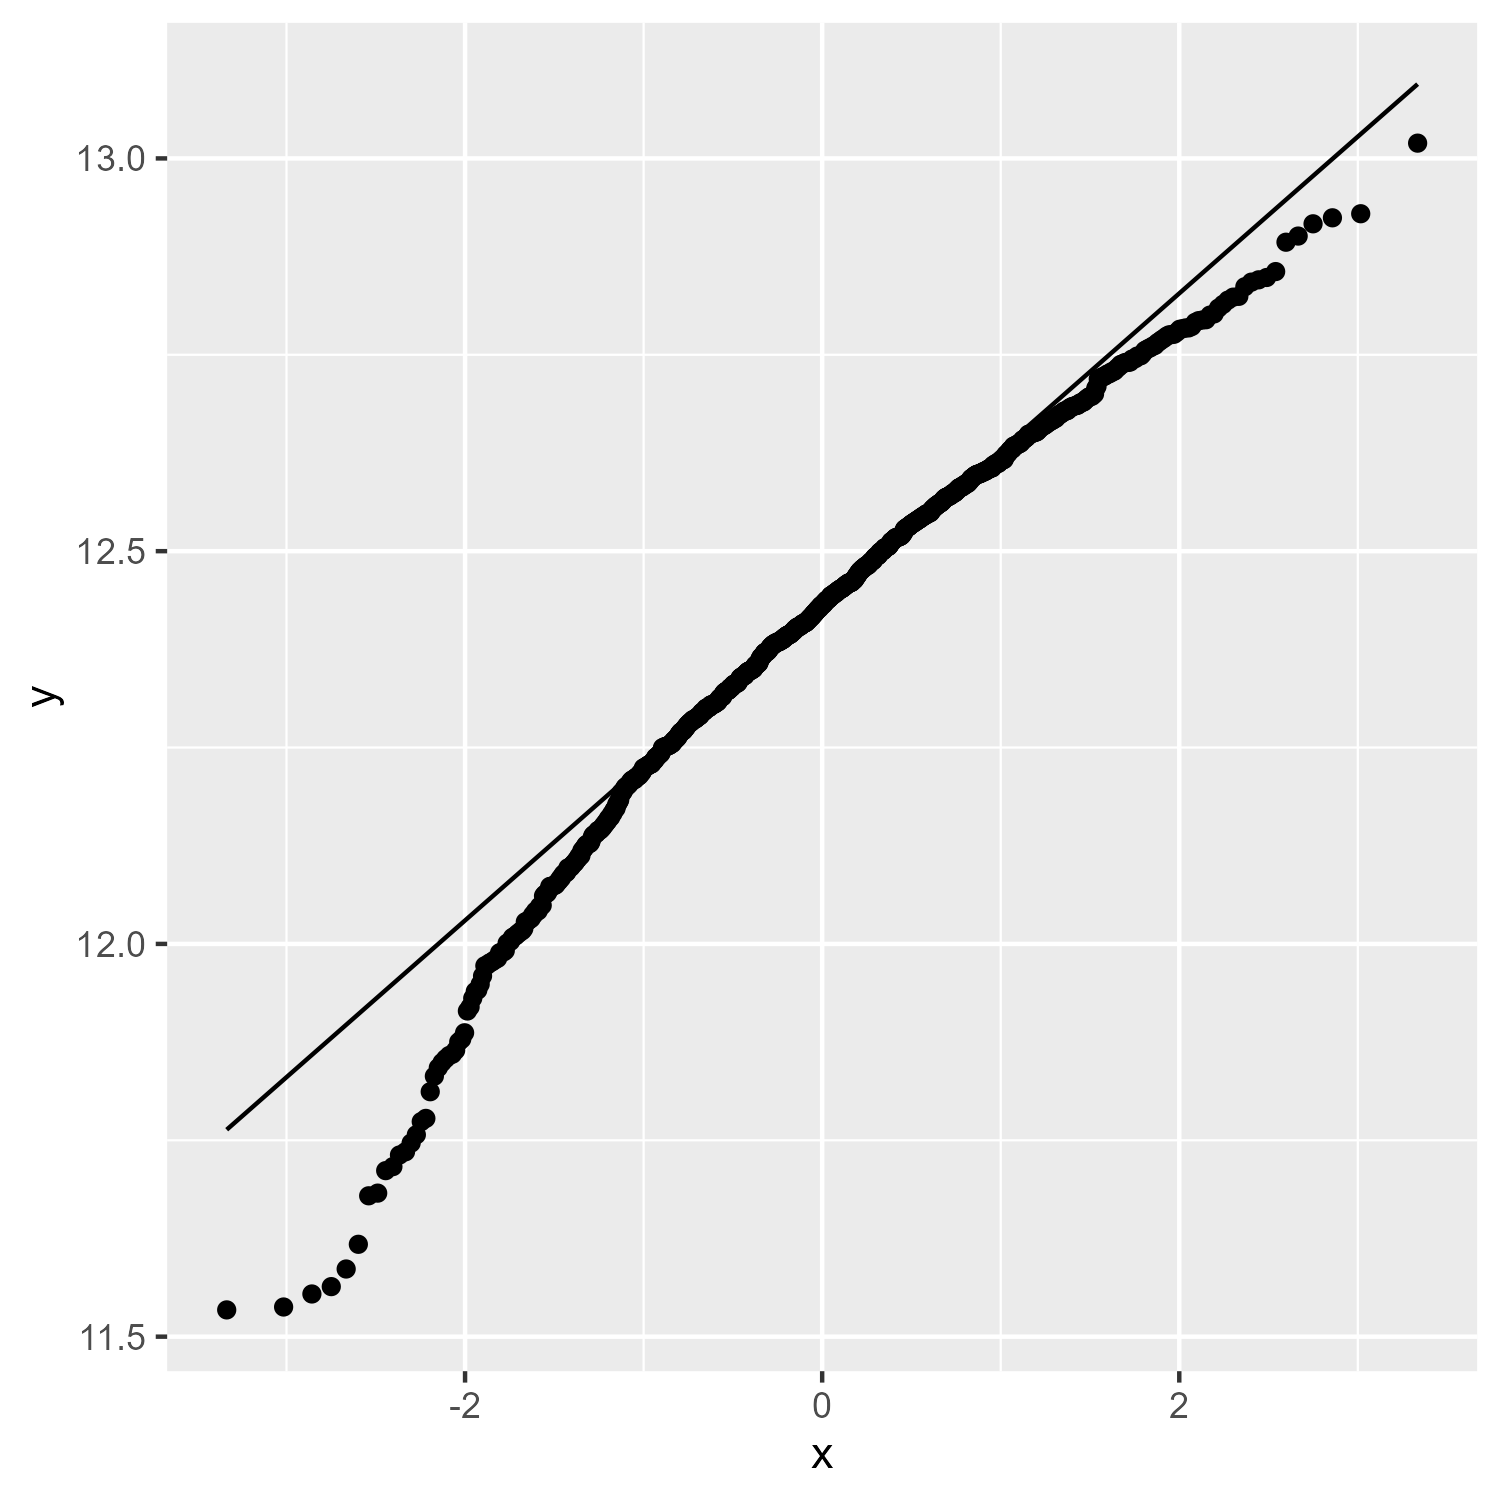
\includegraphics[width=.9\linewidth]{plots/claim_type1/qqplot_lognormality.png}
      \caption{Lognormal fit.}
    \end{subfigure}%
    \begin{subfigure}{.5\textwidth}
      \centering
      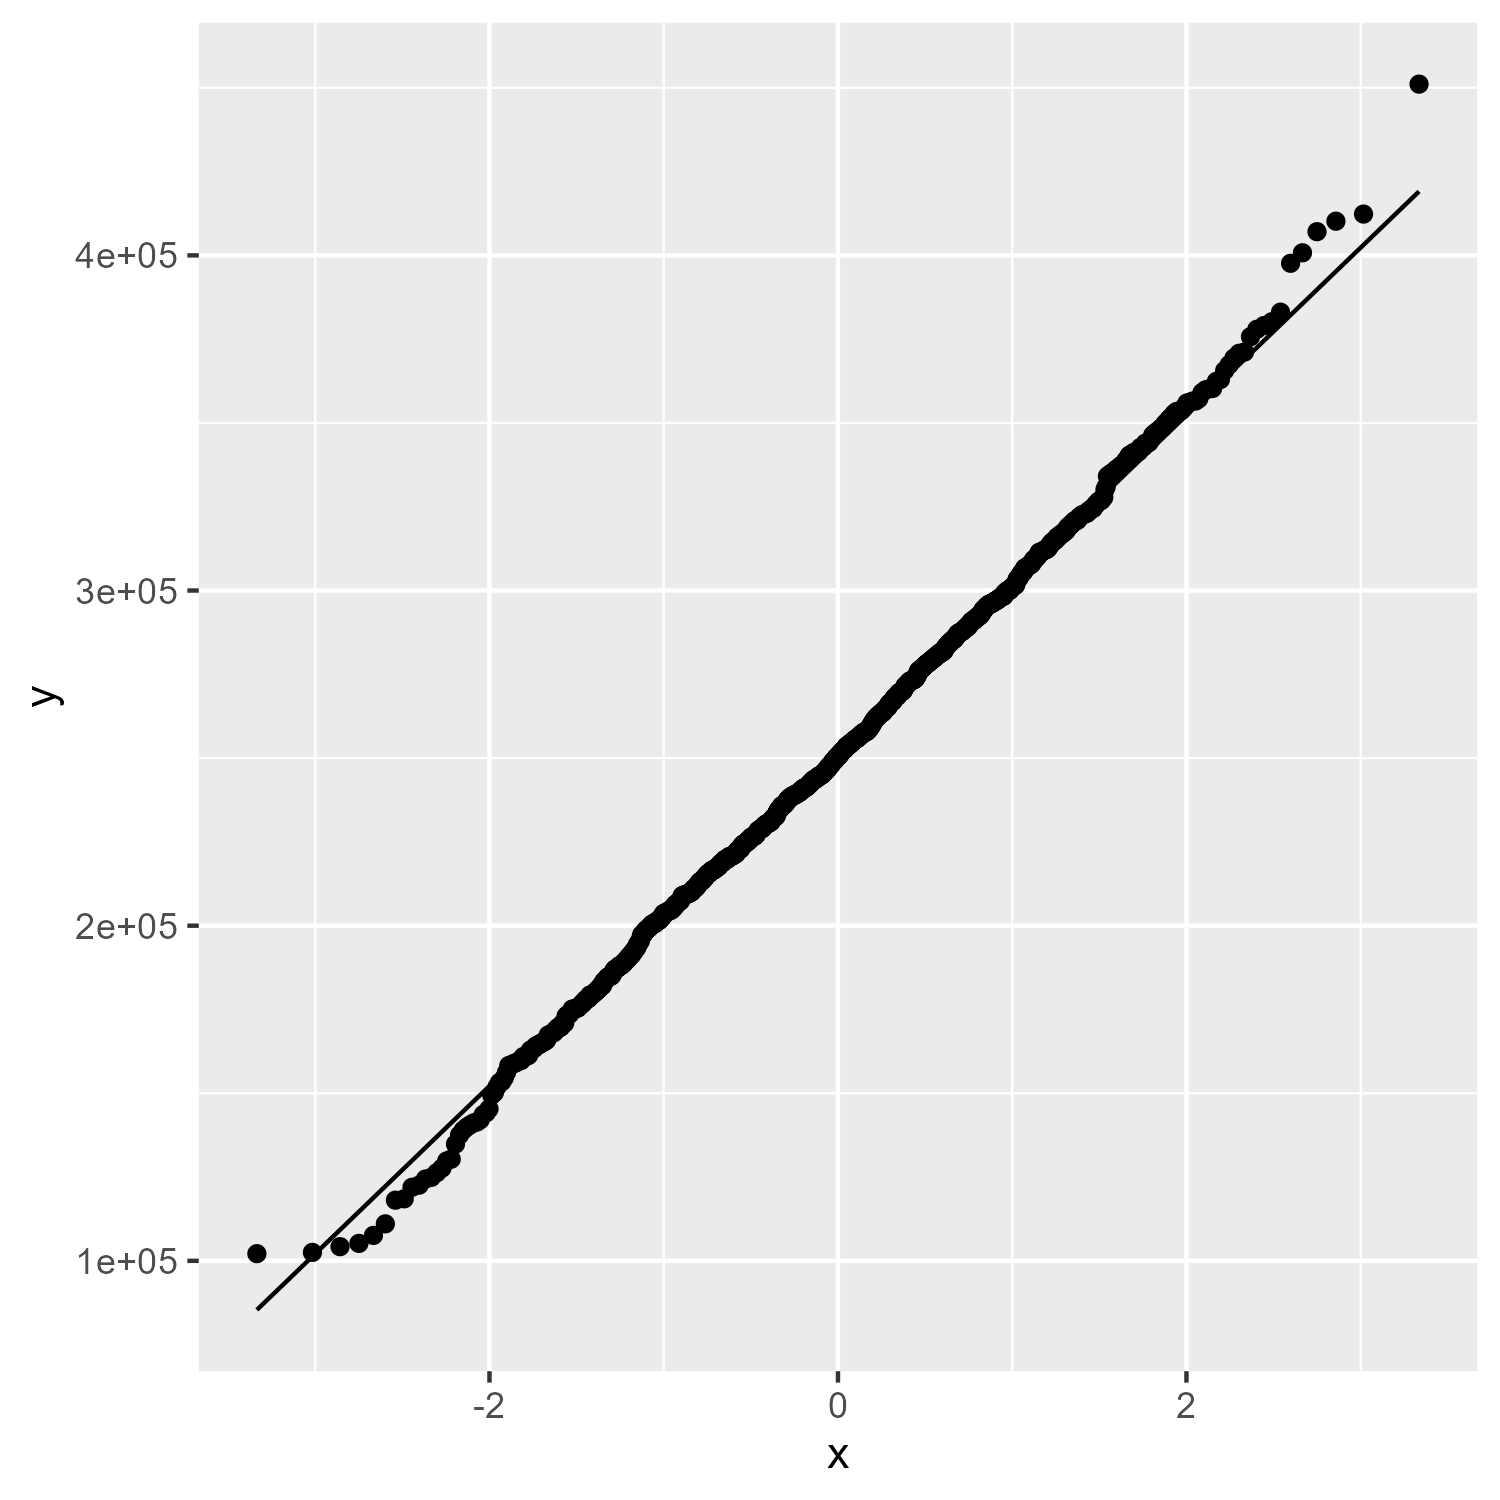
\includegraphics[width=.9\linewidth]{plots/claim_type1/qqplot_normality.png}
      \caption{Normal fit.}
    \end{subfigure}
    \caption{QQ-plots of large branch 1 claims.}
\end{subfigure}
\begin{subfigure}{0.49\textwidth}
    \begin{subfigure}{.5\textwidth}
      \centering
      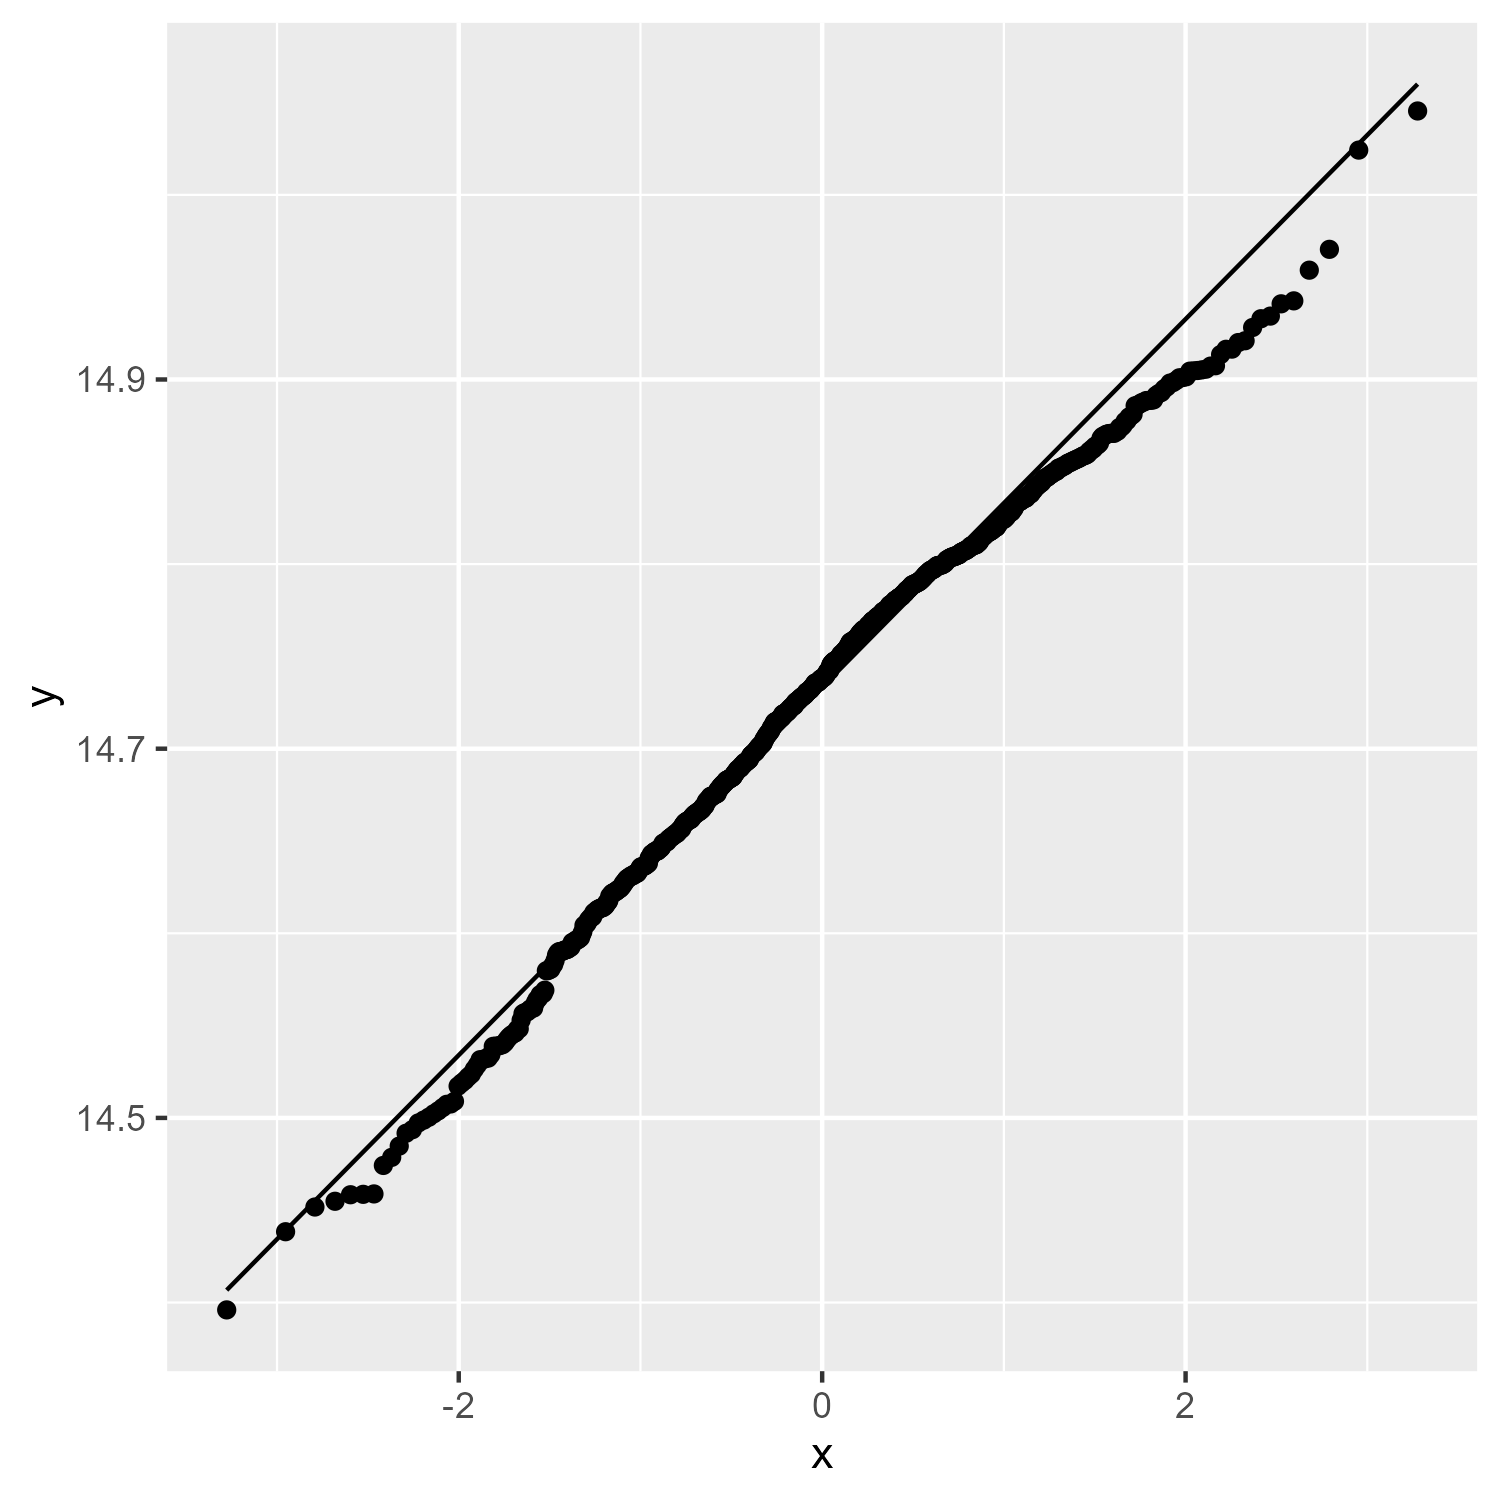
\includegraphics[width=.9\linewidth]{plots/claim_type2/qqplot_lognormality.png}
      \caption{Lognormal fit.}
    \end{subfigure}%
    \begin{subfigure}{.5\textwidth}
      \centering
      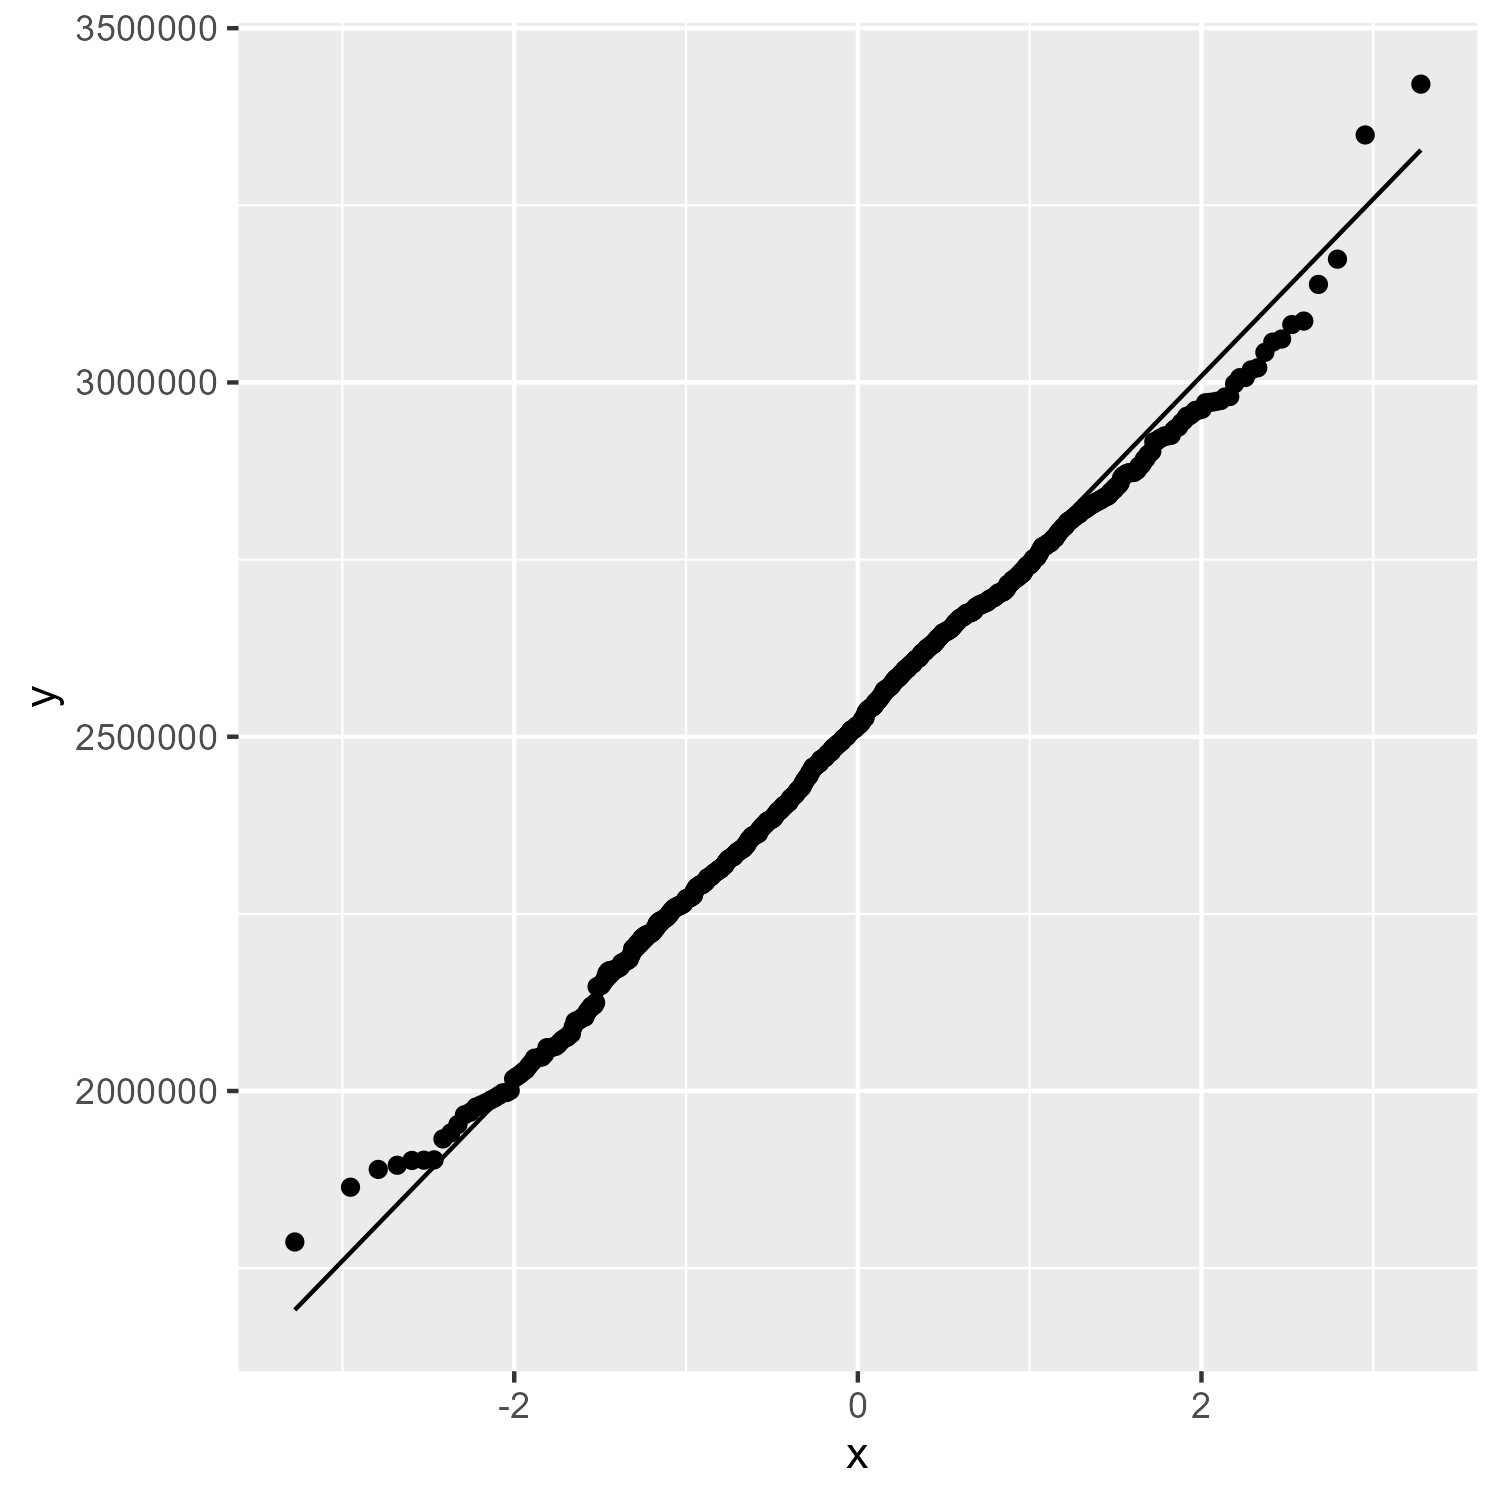
\includegraphics[width=.9\linewidth]{plots/claim_type2/qqplot_normality.png}
      \caption{Normal fit.}
    \end{subfigure}
    \caption{QQ-plots of large branch 2 claims.}
\end{subfigure}
    \caption{QQ-Plots of the large claims in both branches.}
    \label{a2:largeqq}
\end{figure}

Studying the small claims, as seen in figure \ref{a2:smallqq}, we observed that the claims was log-normally distributed. 
Again this was validated through a Kolmogorov–Smirnov test and no significant covariance where found using glm regression using log-normal distribution.
We also analysed to possibility of the distribution to be gamma distributed with covariance, but found no clear connection there either.


\begin{figure}[!h]
\centering
\begin{subfigure}{.49\textwidth}
    \begin{subfigure}{.5\textwidth}
      \centering
      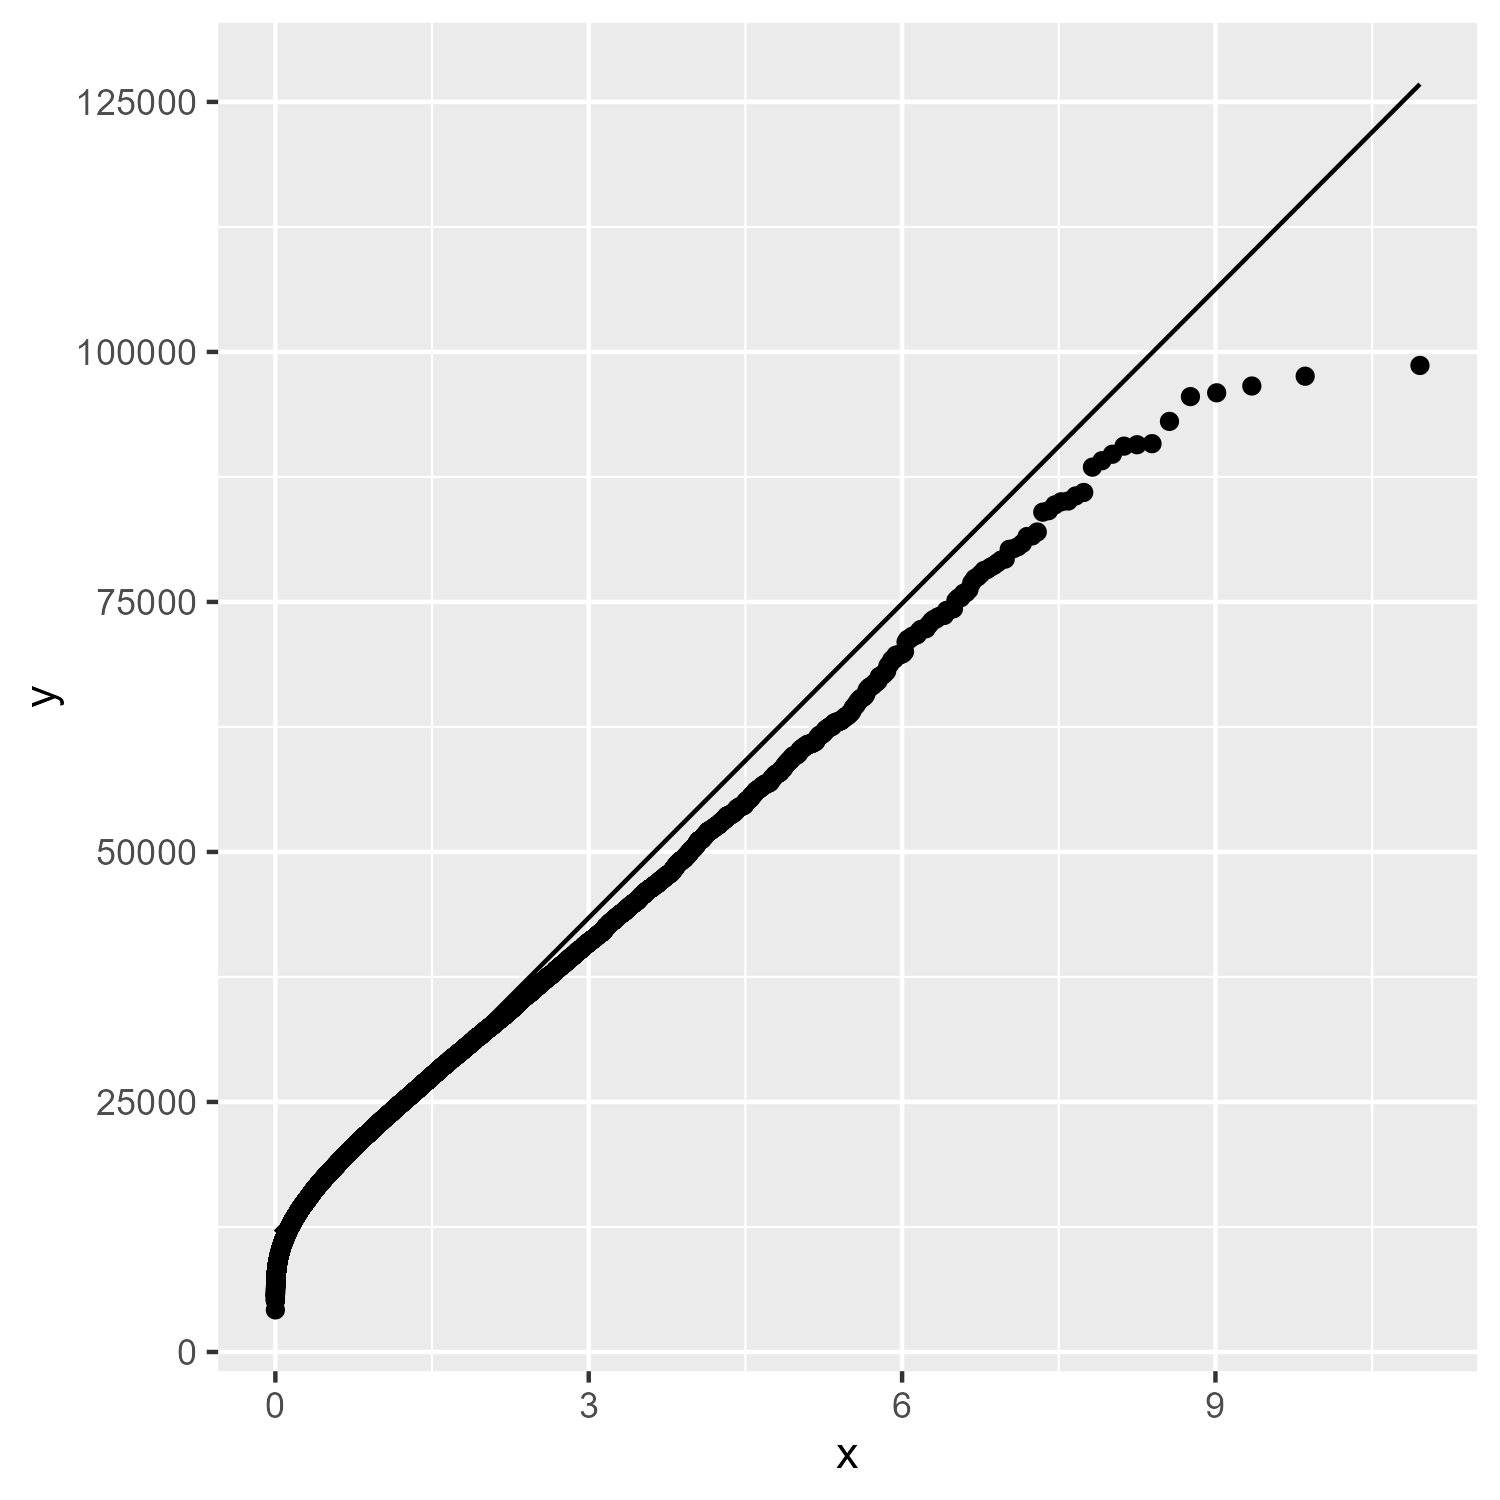
\includegraphics[width=.9\linewidth]{plots/claim_type1/qqplot_gamma_small.png}
      \caption{Gamma fit.}
    \end{subfigure}%
    \begin{subfigure}{.5\textwidth}
      \centering
      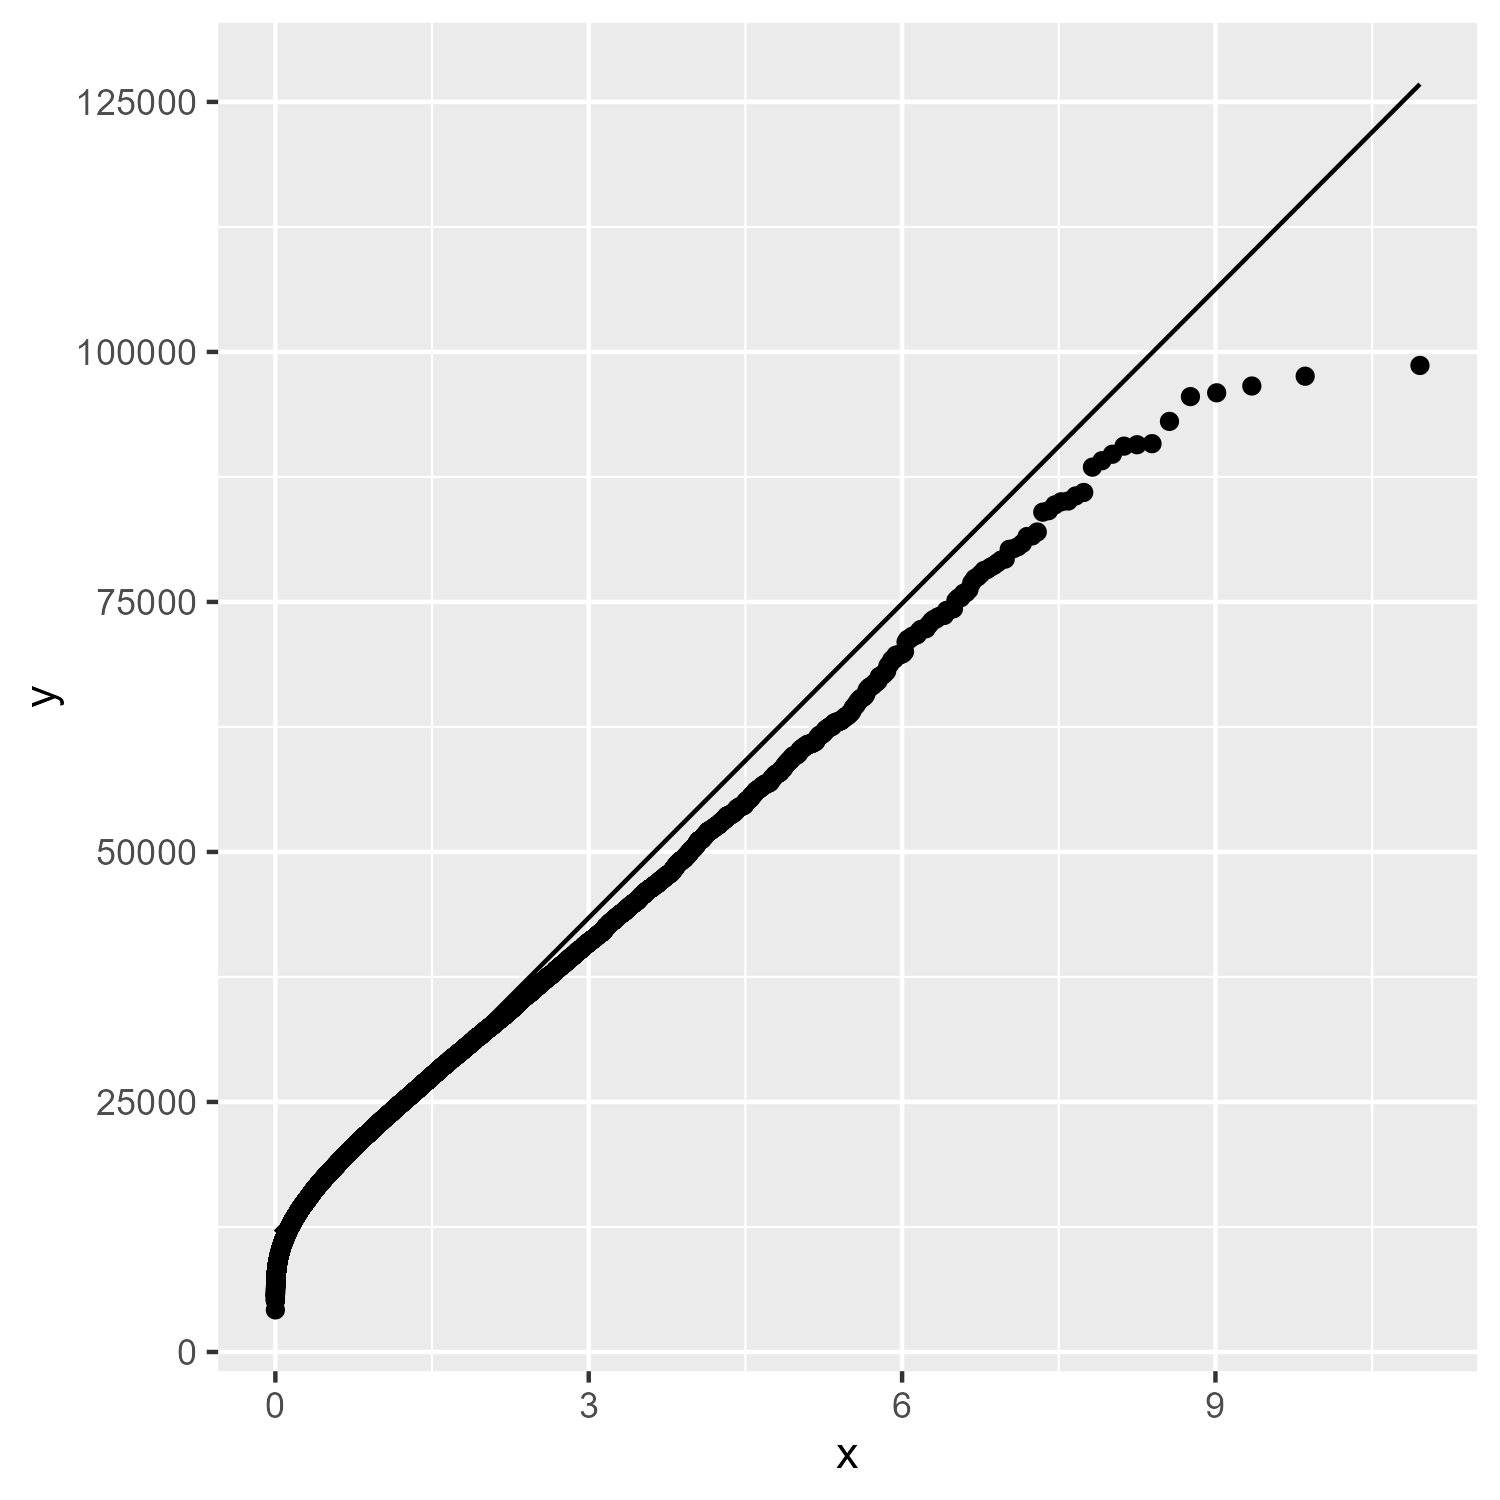
\includegraphics[width=.9\linewidth]{plots/claim_type1/qqplot_weibull_small.png}
      \caption{Weibull fit.}
    \end{subfigure}
    \begin{subfigure}{.5\textwidth}
      \centering
      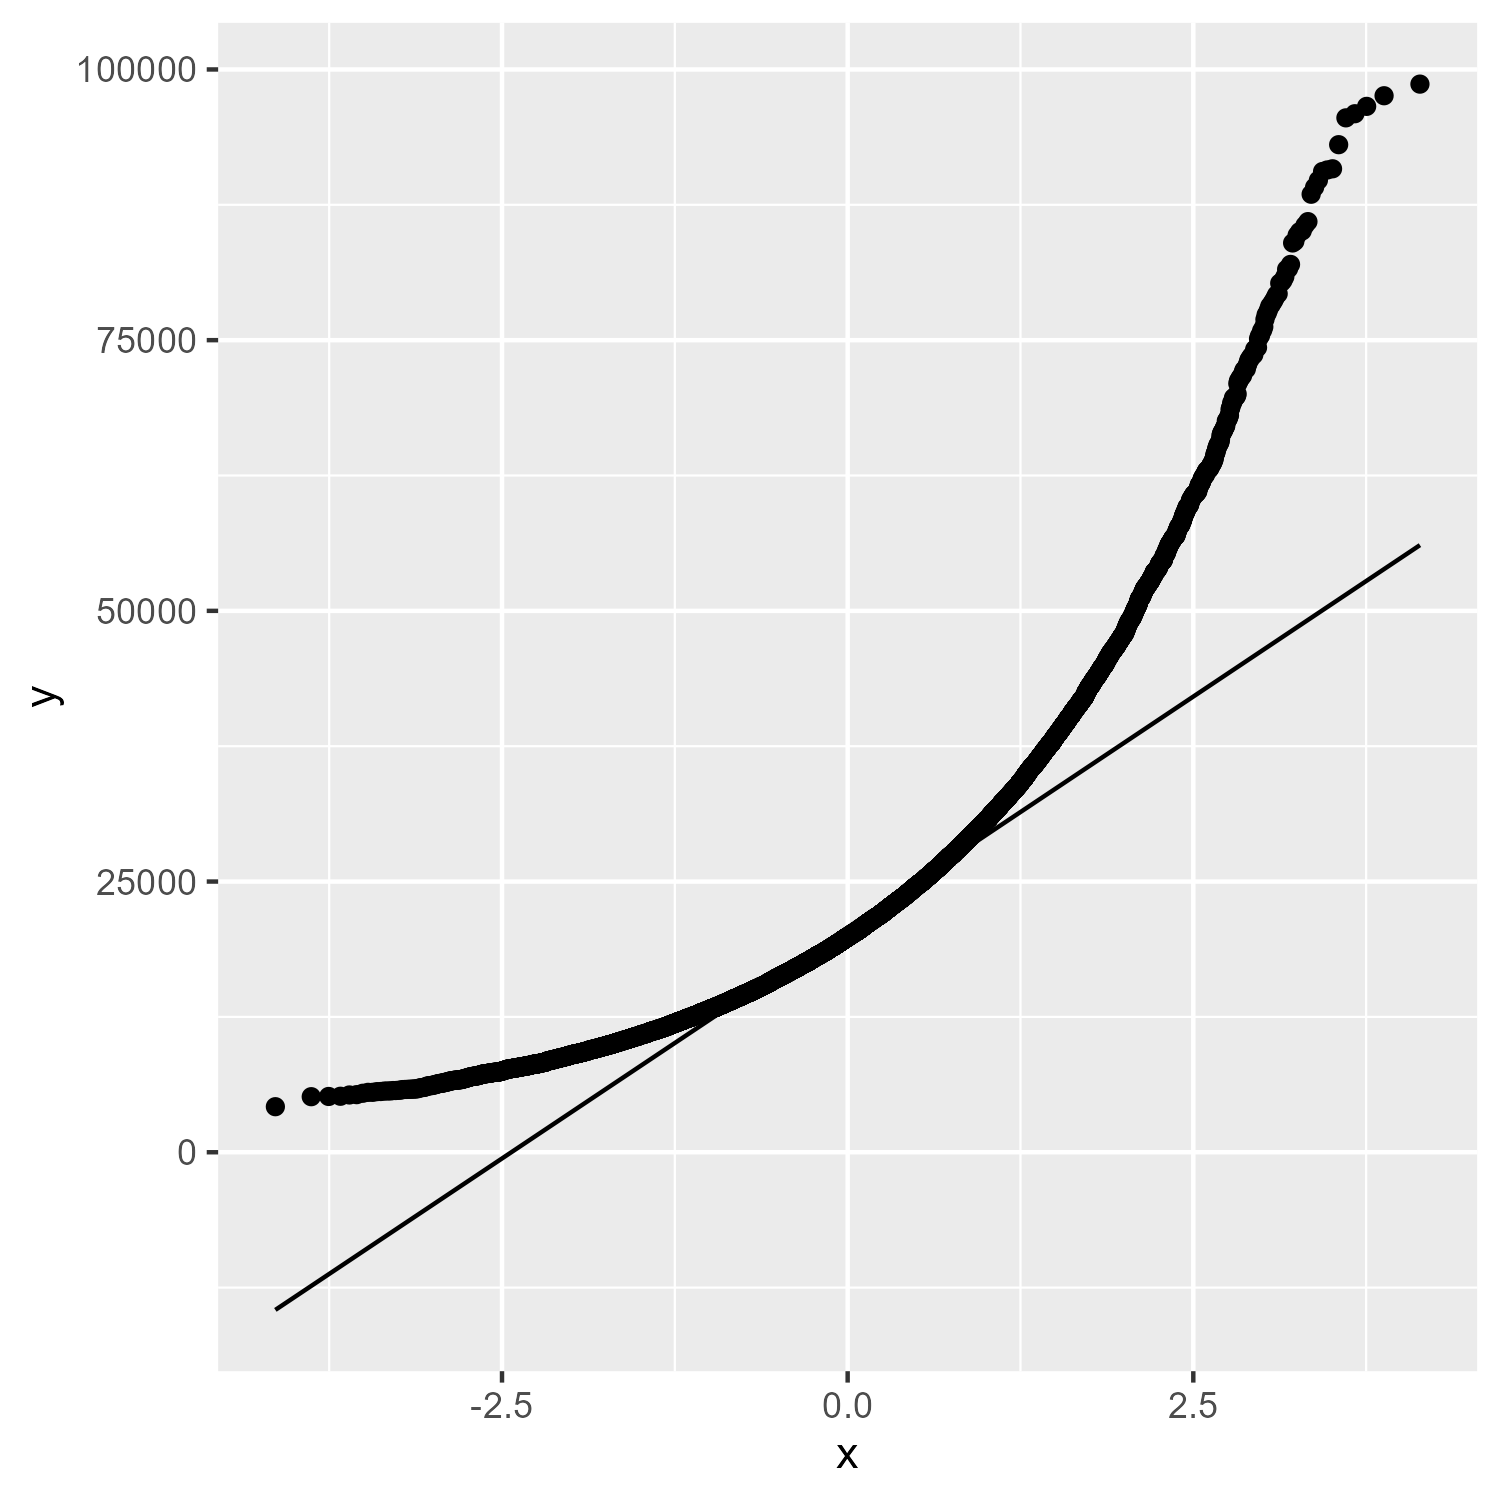
\includegraphics[width=.9\linewidth]{plots/claim_type1/qqplot_normal_small.png}
      \caption{Normal fit.}
    \end{subfigure}%
    \begin{subfigure}{.5\textwidth}
      \centering
      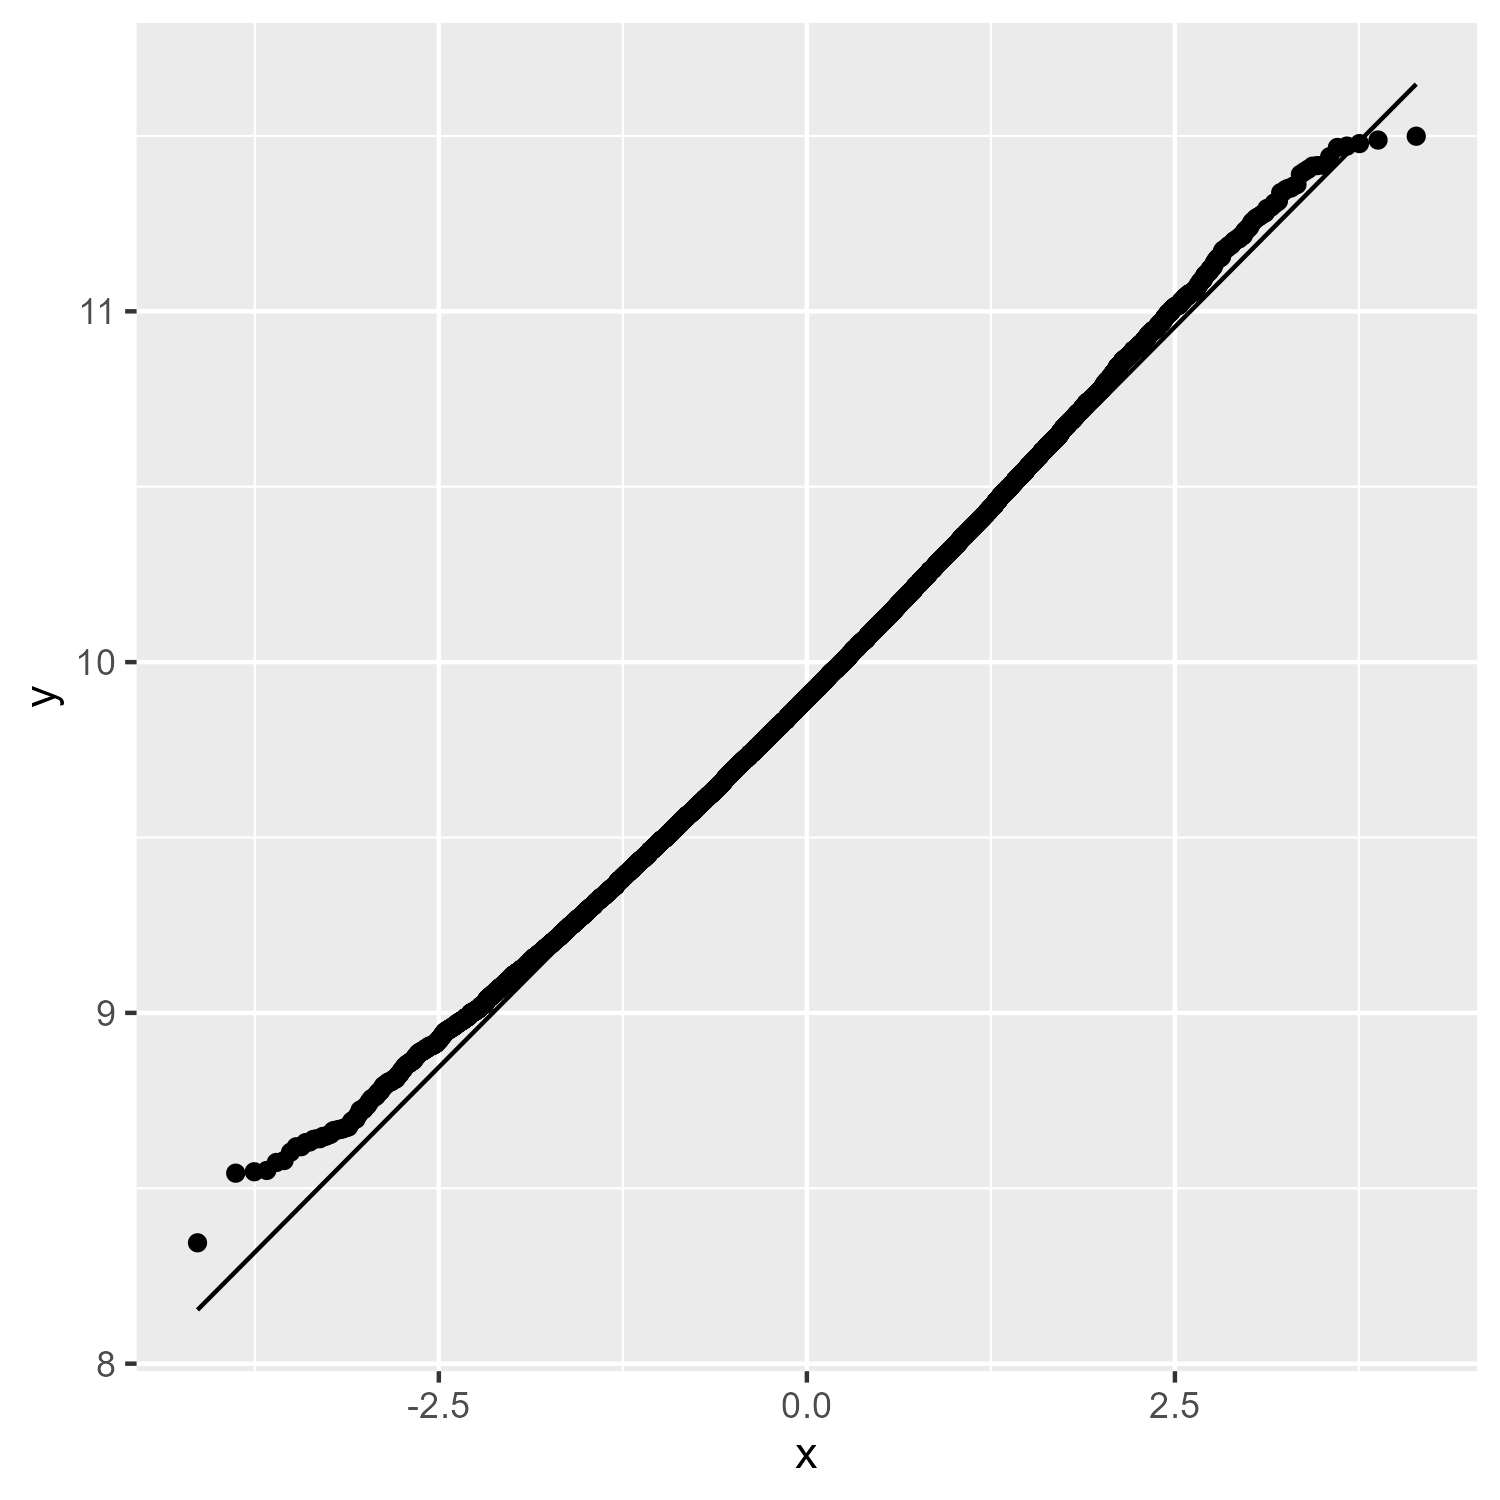
\includegraphics[width=.9\linewidth]{plots/claim_type1/qqplot_lognormality_small.png}
      \caption{Lognormal fit.}
    \end{subfigure}
    \caption{QQ-plots of small branch 1 claims.}
\end{subfigure}
\begin{subfigure}{.49\textwidth}
    \begin{subfigure}{.5\textwidth}
      \centering
      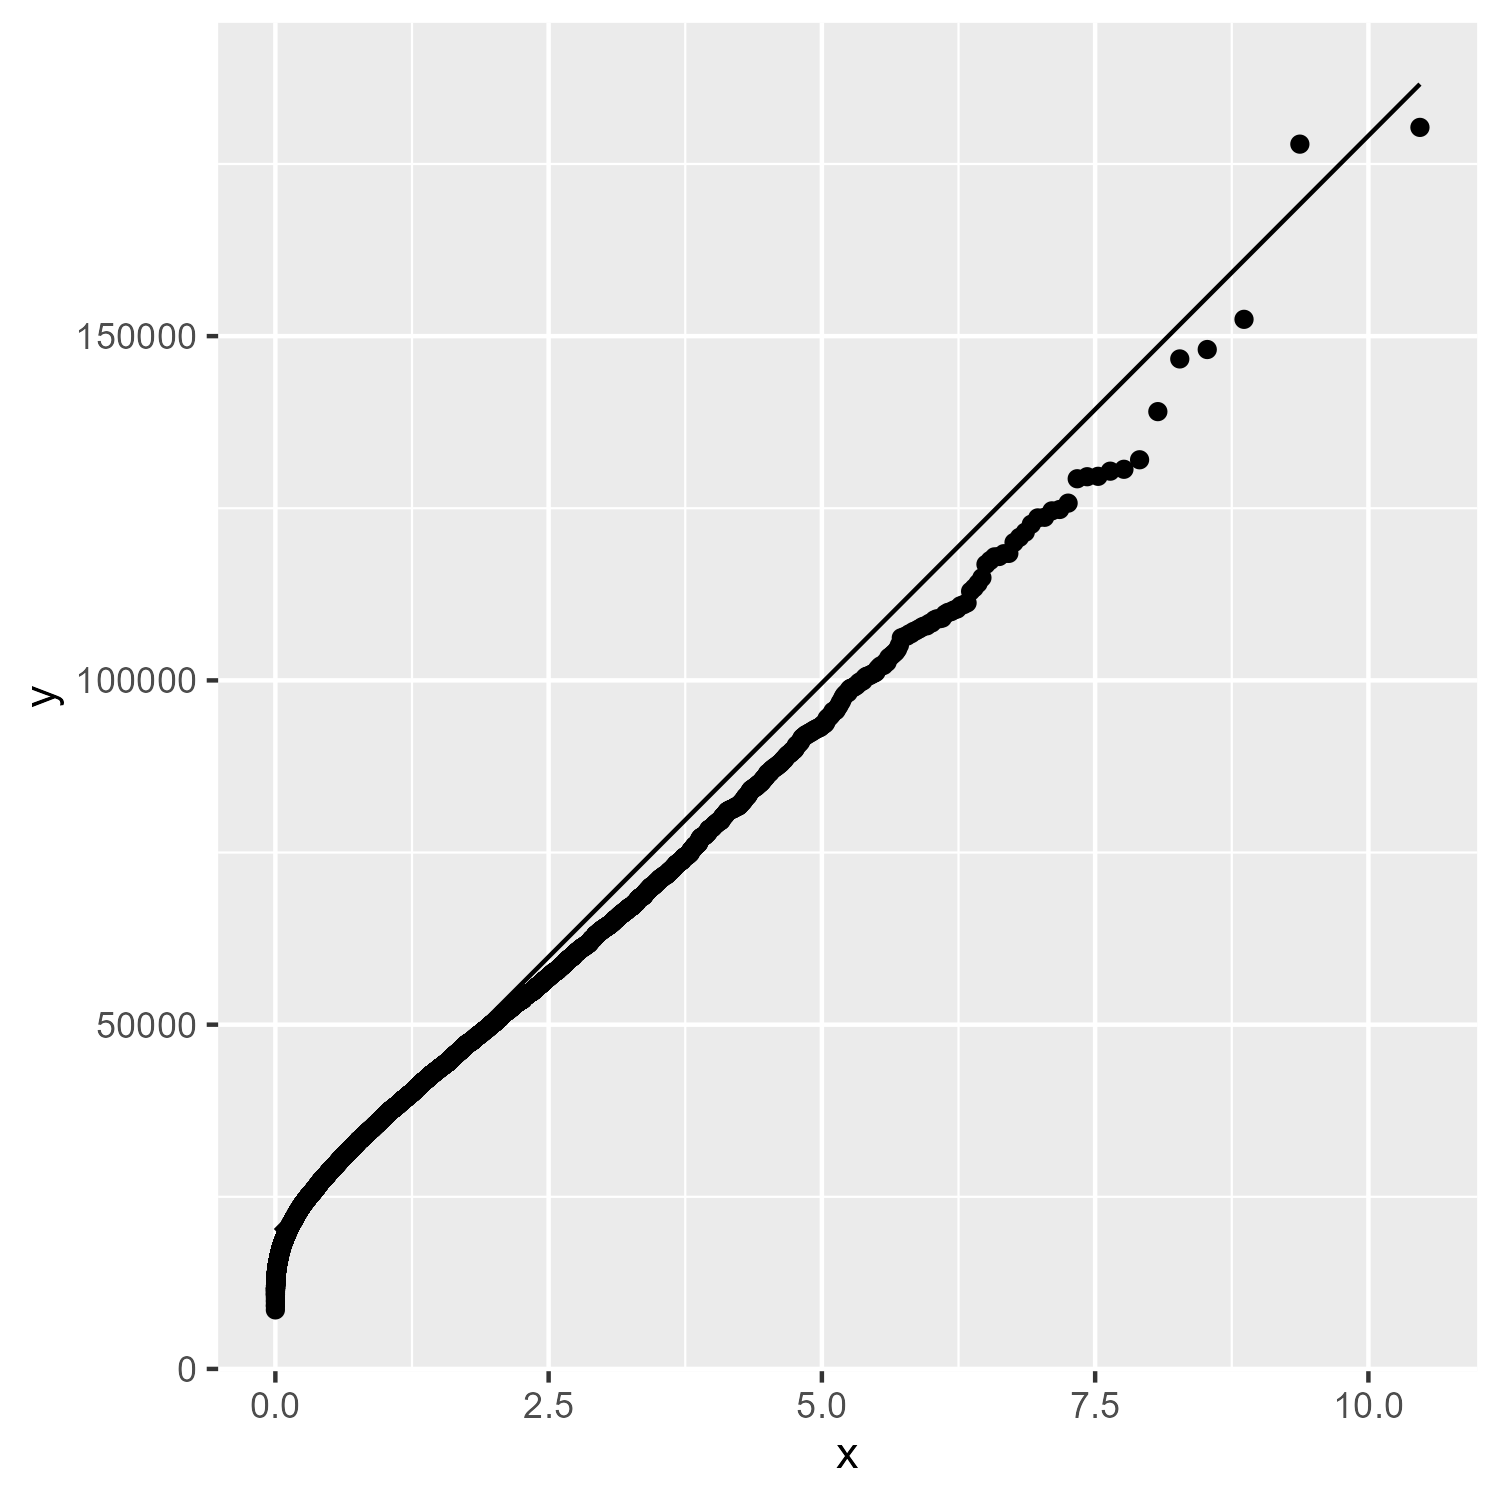
\includegraphics[width=.9\linewidth]{plots/claim_type2/qqplot_gamma_small.png}
      \caption{Gamma fit.}
    \end{subfigure}%
    \begin{subfigure}{.5\textwidth}
      \centering
      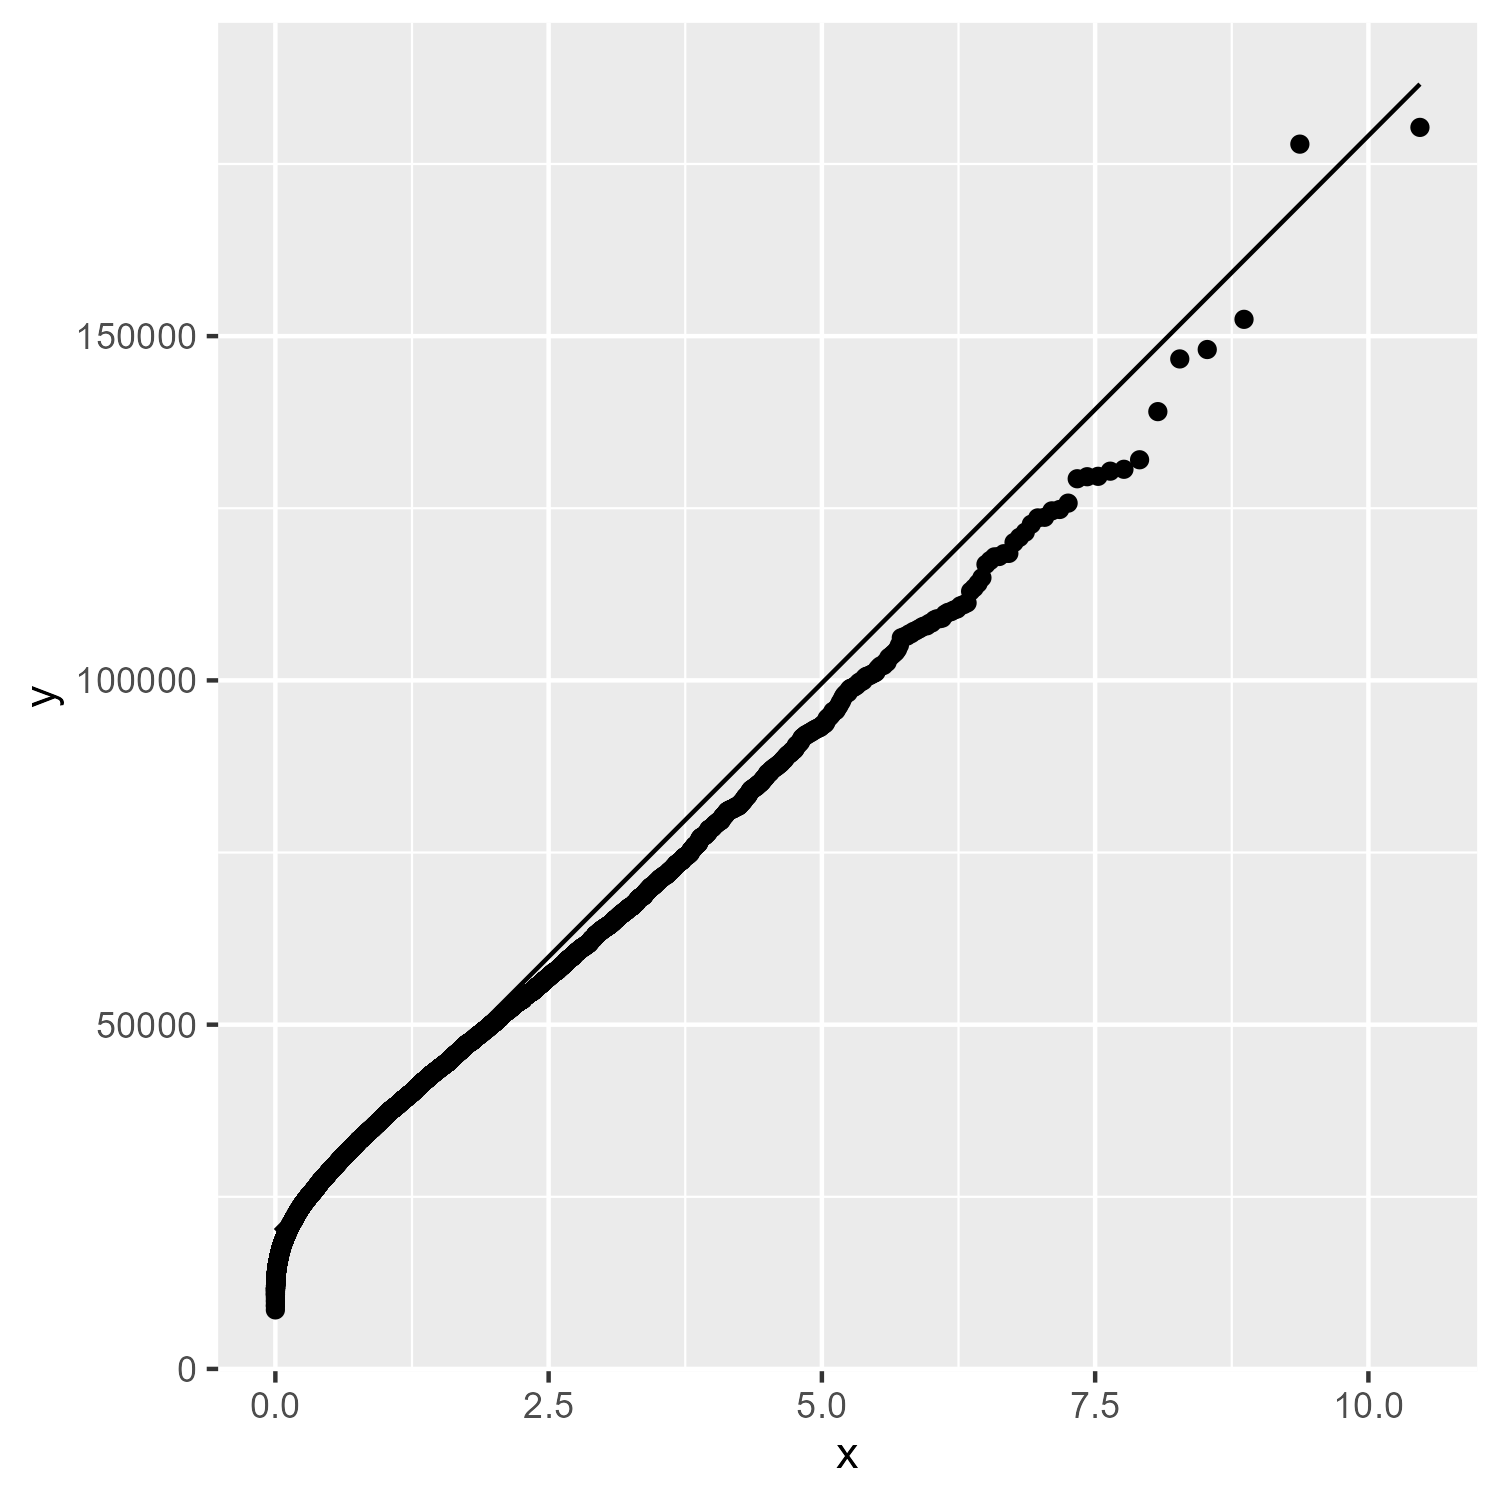
\includegraphics[width=.9\linewidth]{plots/claim_type2/qqplot_weibull_small.png}
      \caption{Weibull fit.}
    \end{subfigure}
    \begin{subfigure}{.5\textwidth}
      \centering
      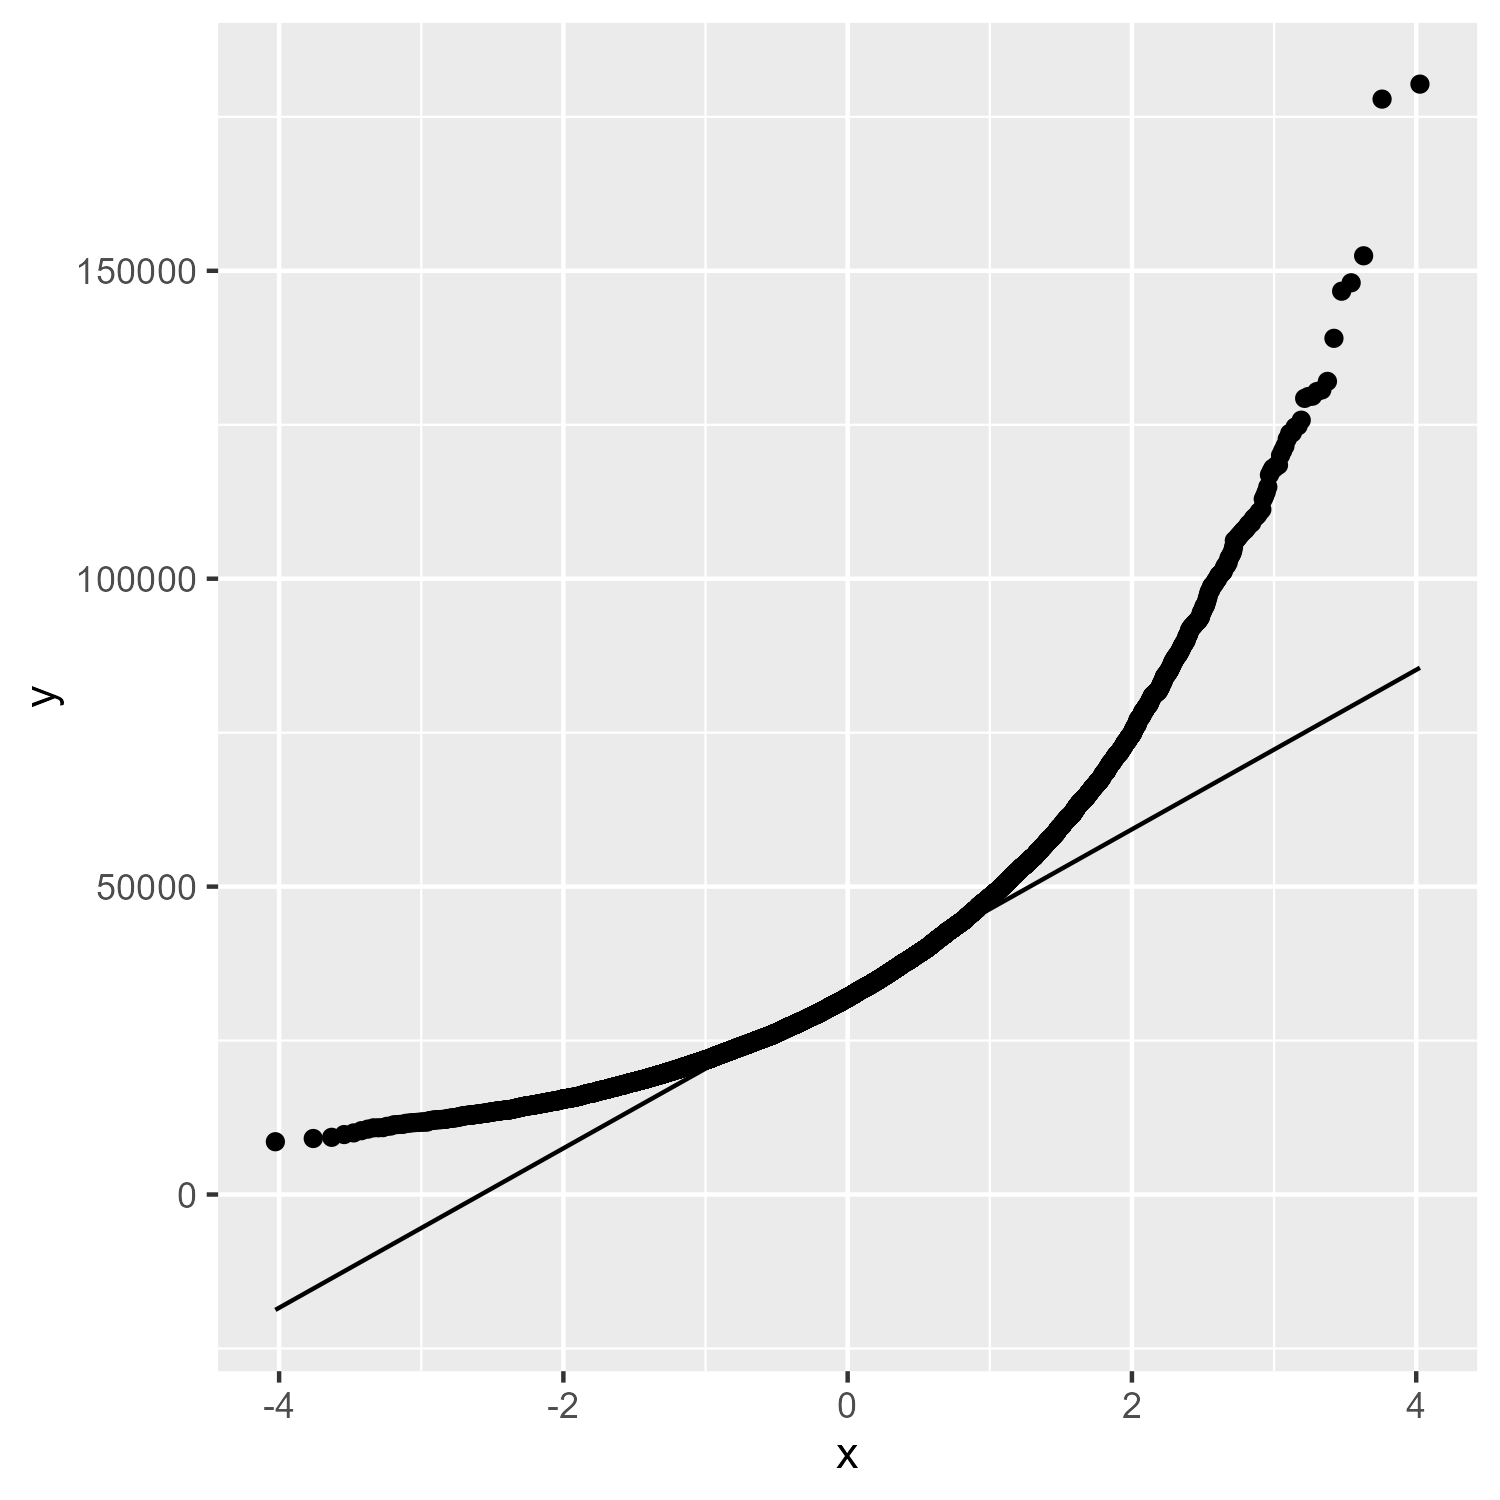
\includegraphics[width=.9\linewidth]{plots/claim_type2/qqplot_normal_small.png}
      \caption{Normal fit.}
    \end{subfigure}%
    \begin{subfigure}{.5\textwidth}
      \centering
      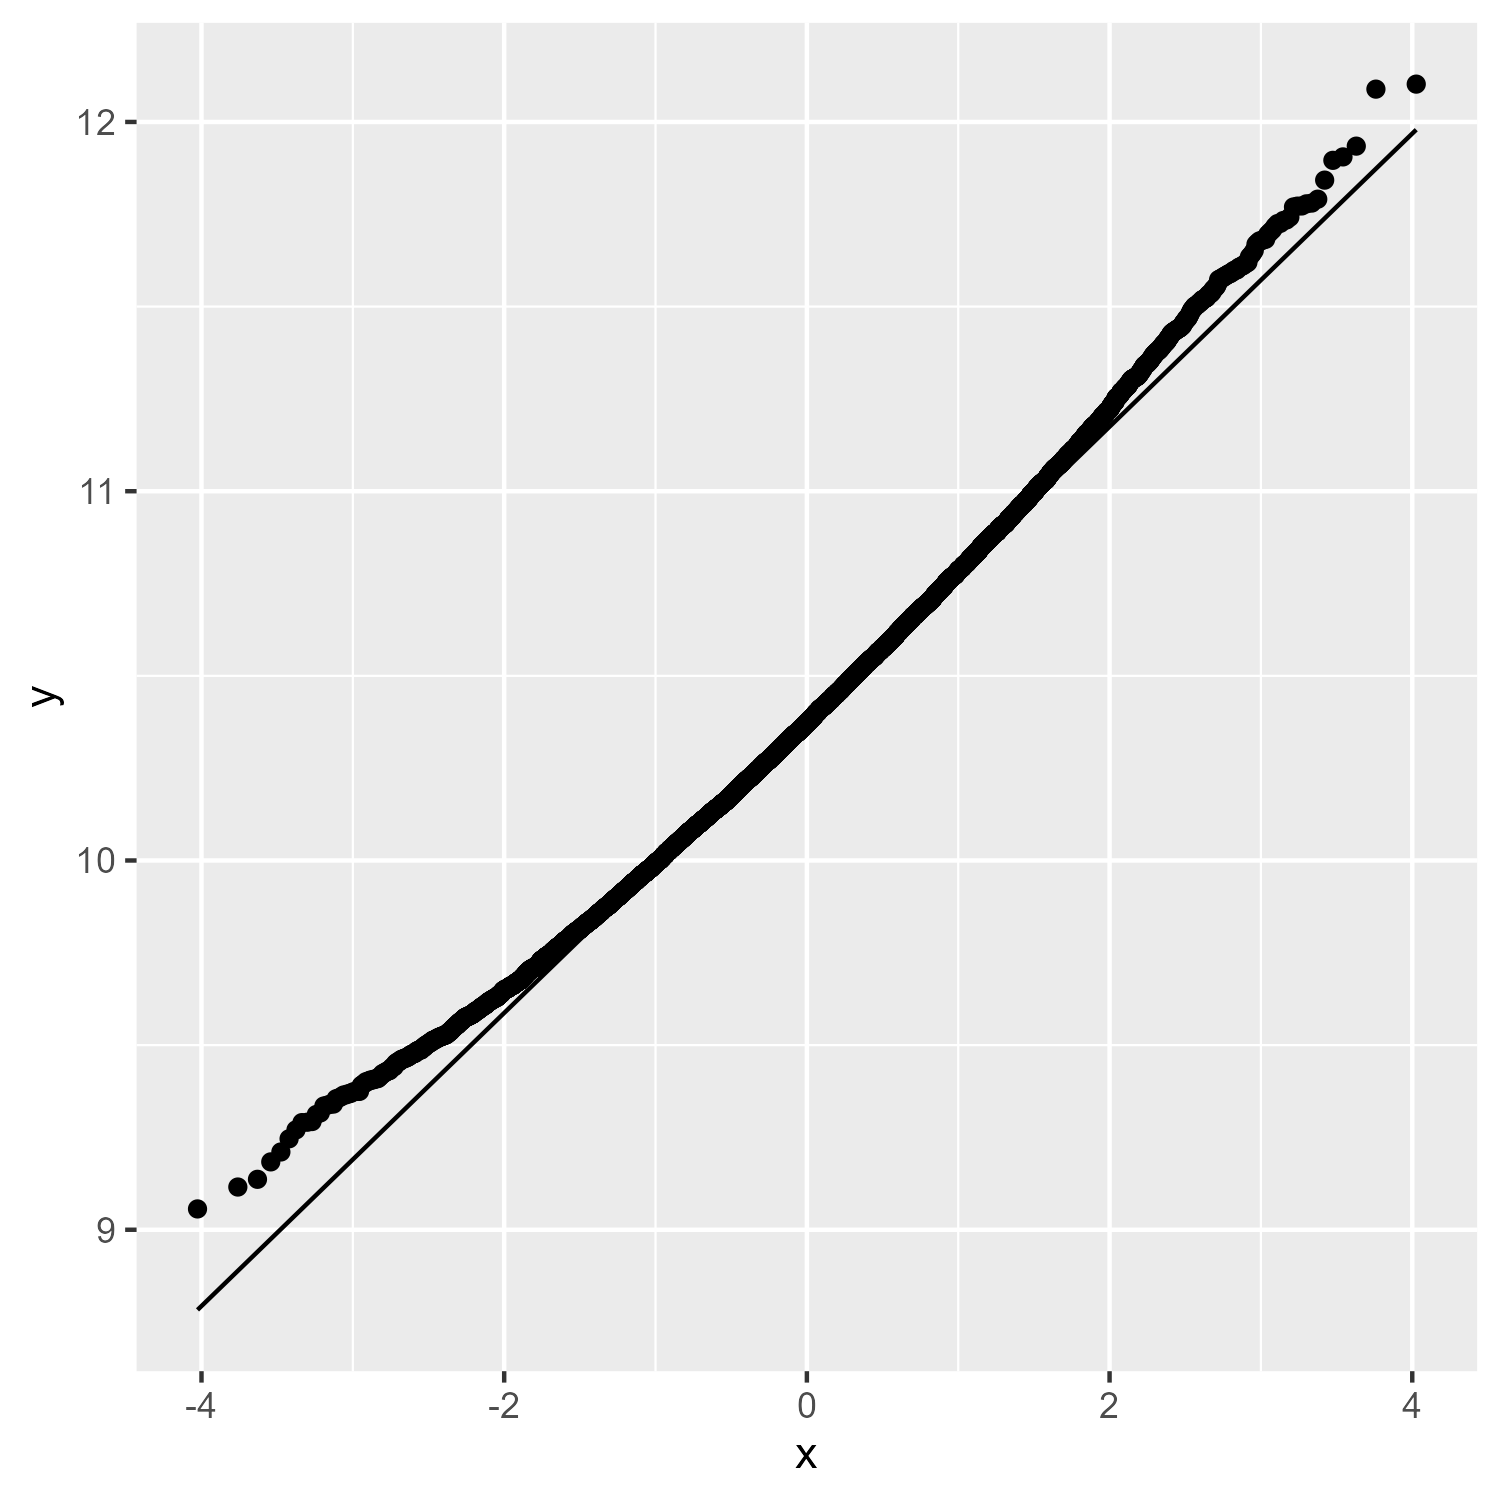
\includegraphics[width=.9\linewidth]{plots/claim_type2/qqplot_lognormality_small.png}
      \caption{Lognormal fit.}
    \end{subfigure}
    \caption{QQ-plots of small branch 2 claims.}
\end{subfigure}
    \caption{QQ-Plots of the small claims in both branches.}
    \label{a2:smallqq}
\end{figure}

In the end we get the final model for our claim severity as

\begin{equation}
    \begin{split}
        p_{i} &\sim Beta(\alpha_i,\beta_i)  \\
        S_{i,small} &\sim LogNormal(\mu_{i,small},\sigma_{i,small}) \\
        S_{i,large} &\sim N(\mu_{i,large},\sigma_{i,large})
    \end{split}
\end{equation}

with $i=1,2$ denoting which branch it is.
and we get a total claim size for a given claim in branch $i$

\begin{equation*}
    S_i \sim \begin{cases}
      S_{i,large}  & \text{with probability } p\\
      S_{i,small}  & \text{with probability } 1-p
    \end{cases},  i =1,2
    \label{a2:formula}
\end{equation*}


Do observe that we will estimate $p_i$ using the mle estimate $\alpha_i= N_{i,large}$ and $\beta_i=N_{i,small}$, but for the simulations we will use a single mle estimate of $p$ as the expected value $\hat{p}=\frac{\alpha_i}{\alpha_i+\beta_i}$, therefor not draw a probability from this distribution.

This modeling is all conditional on that a claim has occurred, and assuming that all claims are independent with no auto-correlation between claims.
We will now go deeper into the arrival process, and assume that that there is no correlation between claim frequency and severity, model how claims arrive.

\subsection*{Dependency between branches}
Before combining the exploratory research into a single model we study the dependency between the branches.
Aggregating the data and studying the number of claims and size seen in figure \ref{a3:claimamount} and \ref{a3:claimcount}, we observe from that there see be a correlation between the branches.
This could again be a factor of what previously assumed, that branch 1 are motor claims and branch 2 are personal injury claims in regards to motor insurance.
Most likely that data is simulated, but if it was to be similar to any real world data, motor could be a candidate.

\begin{figure}[h!]
    \begin{subfigure}{.49\textwidth}
        \centering
        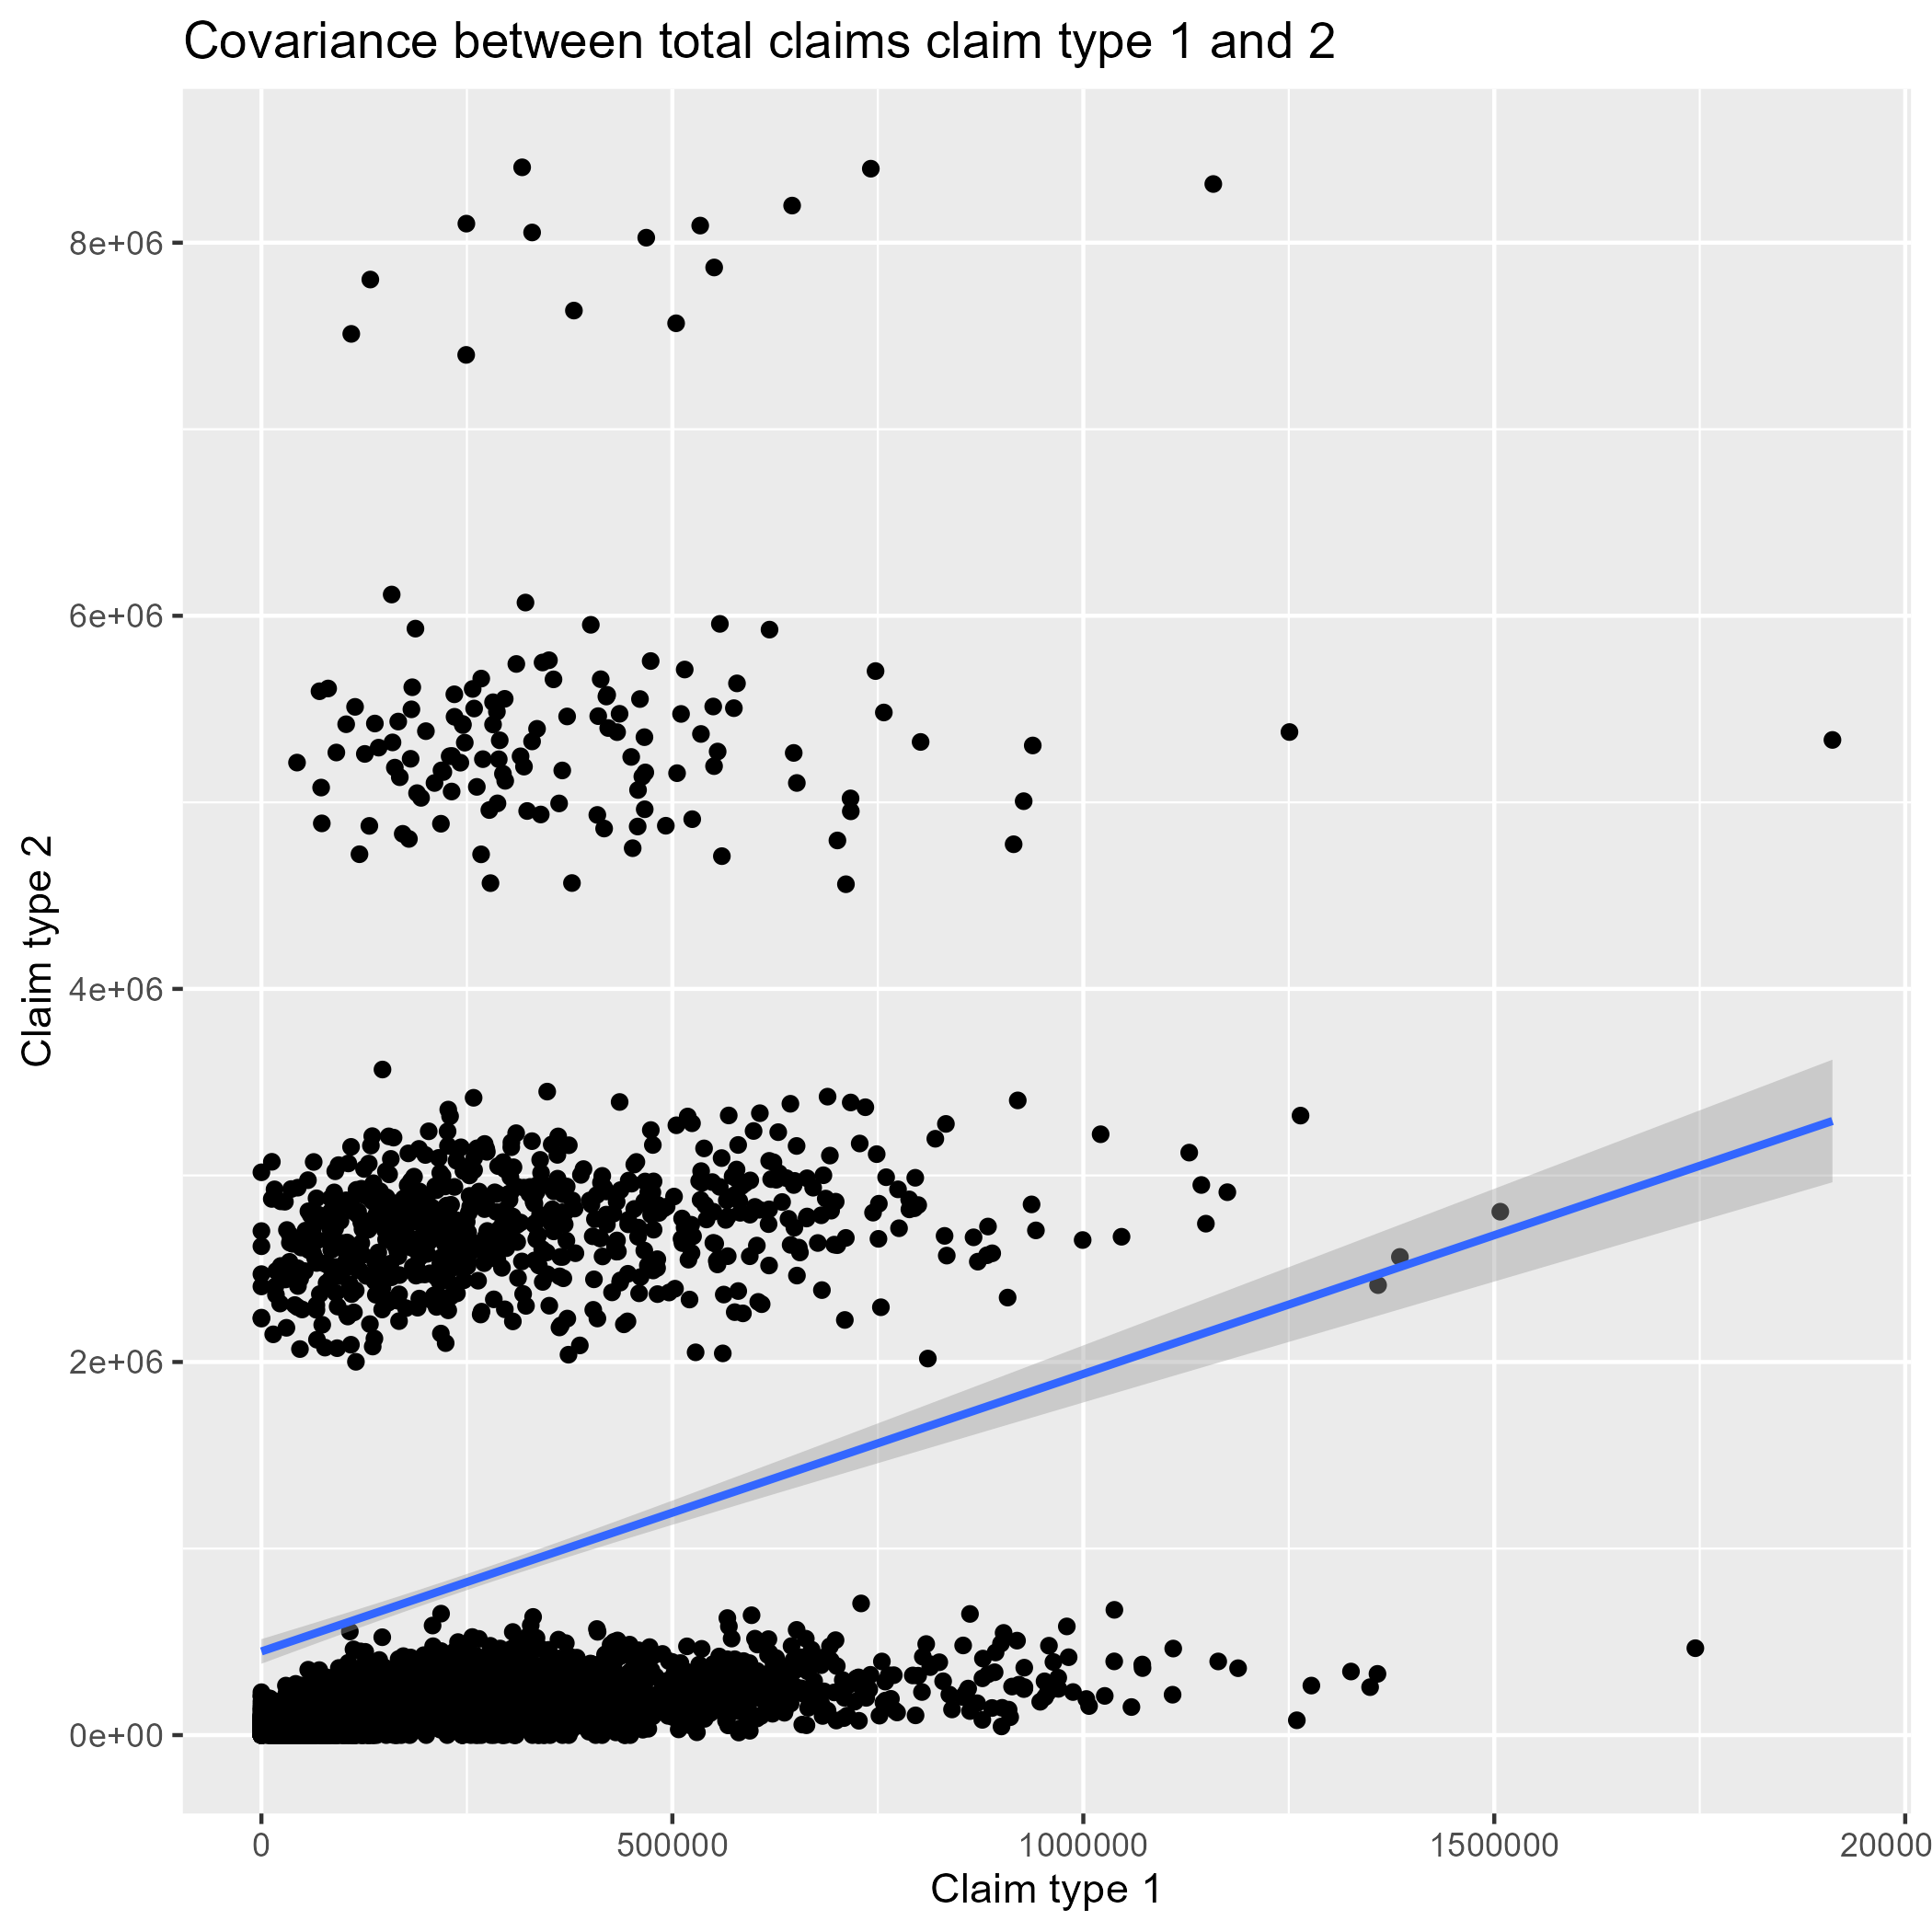
\includegraphics[width=.9\linewidth]{plots/covariance/daily_claim_size.png}
        \caption{Total claim size per day.}
        \label{a3:claimamount}
    \end{subfigure}
    \begin{subfigure}{.49\textwidth}
        \centering
        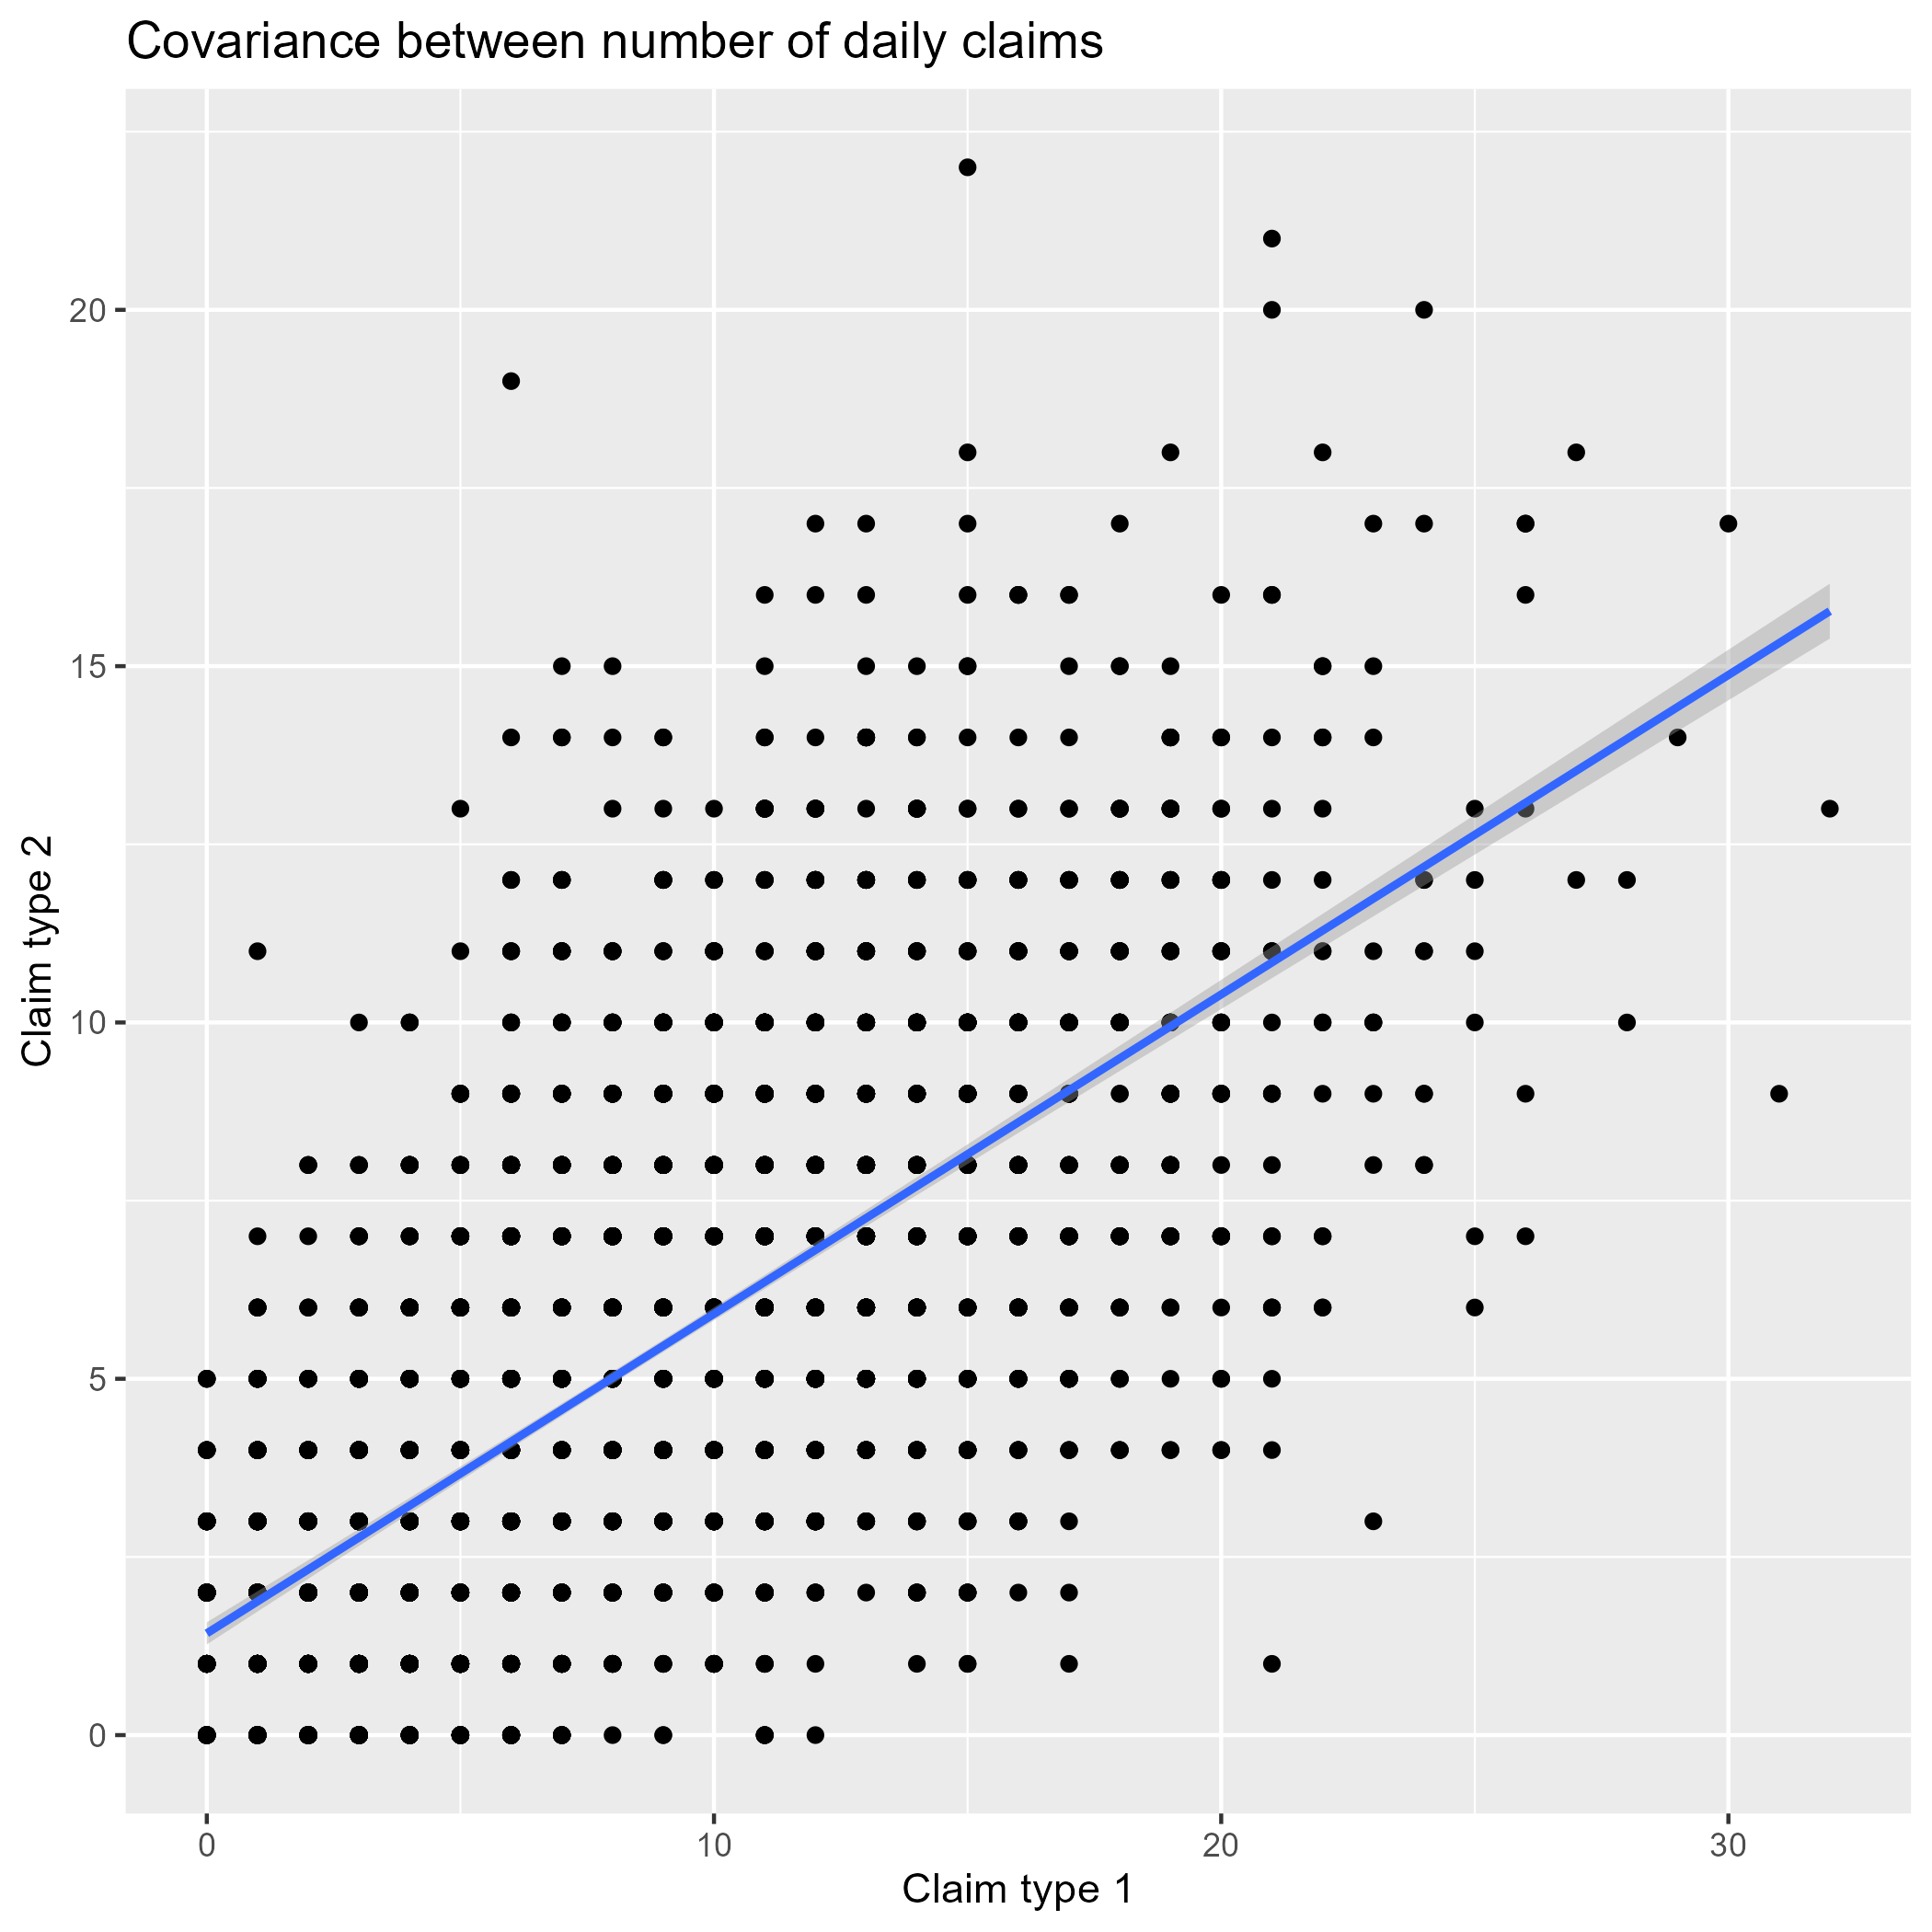
\includegraphics[width=.9\linewidth]{plots/covariance/daily_claim_number.png}
        \caption{Total number of claims per day.}
        \label{a3:claimcount}
    \end{subfigure}
\end{figure}

\begin{wrapfigure}{r}{0.45\textwidth}
  \begin{center}
    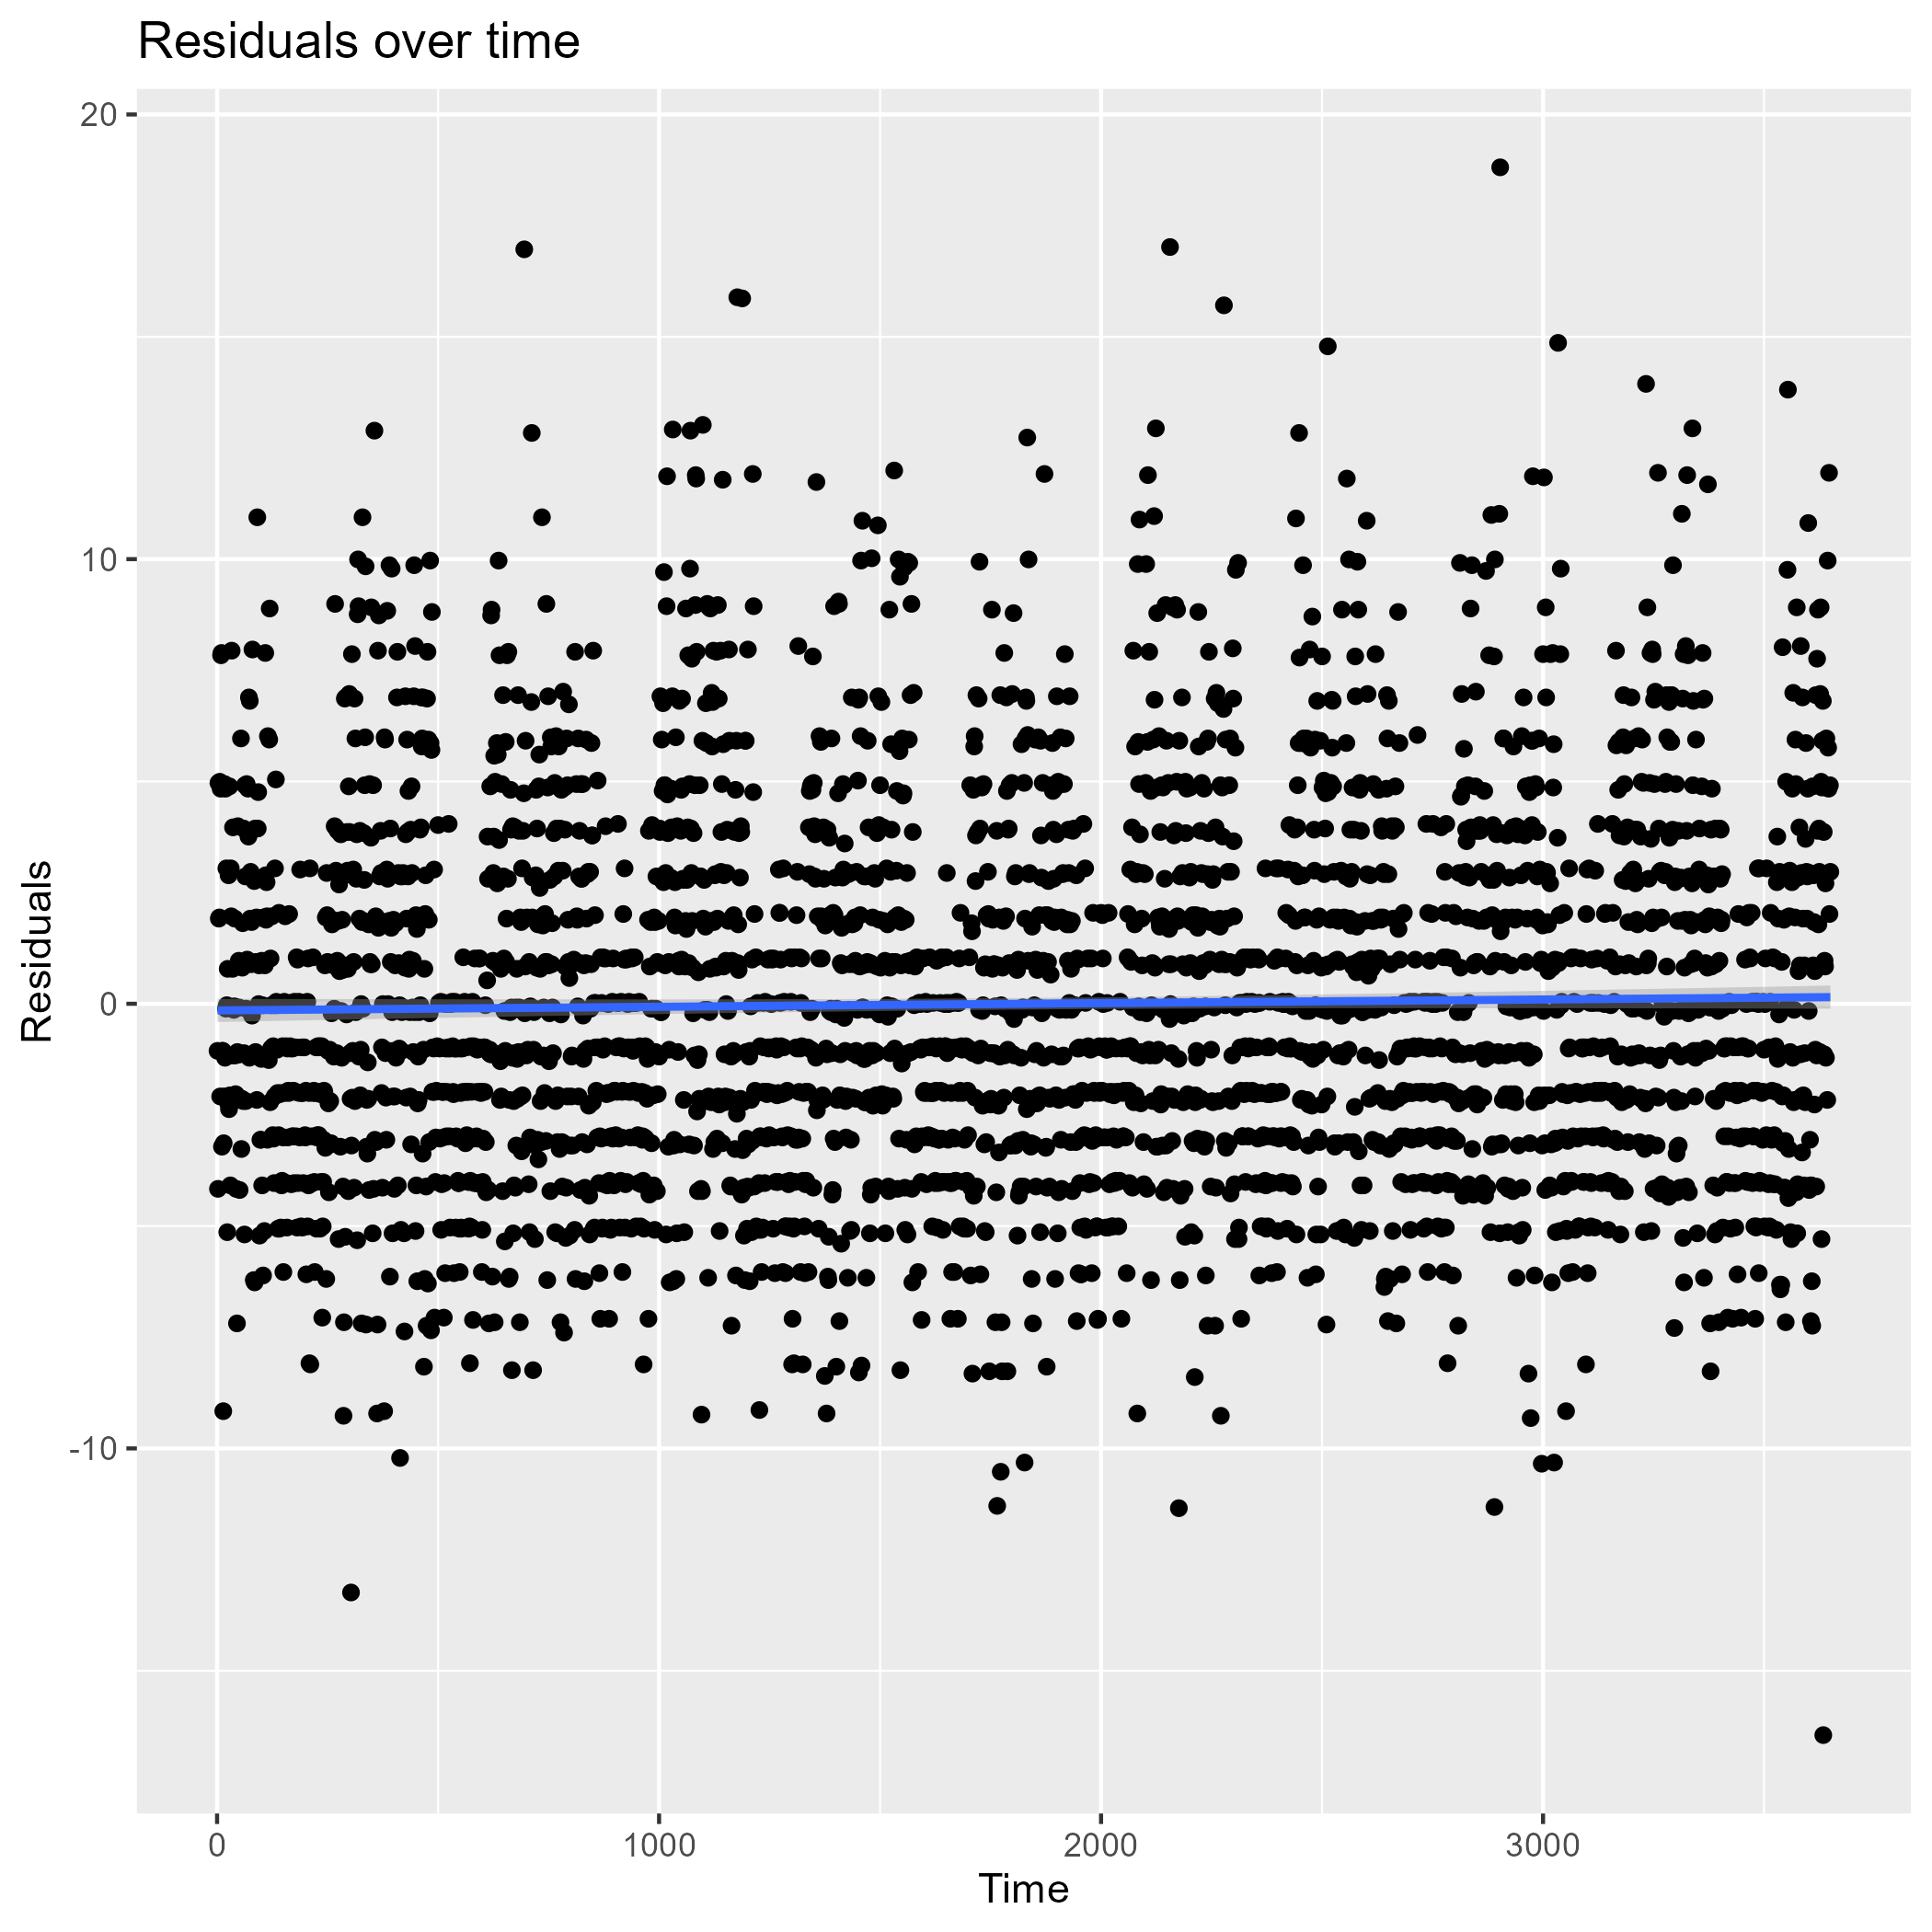
\includegraphics[width=0.45\textwidth]{plots/covariance/count_residual_overTime.png}
  \end{center}
  \caption{Residual of the claim arrival fit.}
  \label{a3:residual}
\end{wrapfigure}

Do observe that the strange pattern in figure \ref{a3:claimamount}, comes as a consequence of the number of large claims in branch 2 per day, and that they are significant larger to the small one compared to branch 1. 
In doing so we observe a cluster in the top that 3 large claims have occurred during a singular day, but there is no occurrence of 4 large claims on a single day.
For branch 1, the large claims are not that significant larger and the effect is less apparent.

Studying the claim amounts we saw no significant effect between the branches, in doing so we studied the average claim size per day, and not the total.
We tested this using a gamma glm regression and found no significant effect between the average claim size.
Instead the correlation was much more apparent studying the claim arrival process.

In studying the arrival process, we observed that the Poisson distribution was not be the best fit, but that the model seem to be over-dispersed.
We tried modeling the arrival process using a negative-binomial distribution but found the quasi-Poisson process to be the best fit for the data.

Using the quasi-Poisson glm we studied the correlating factors and saw significant effect between the branches and that the claim occurred during the summer, as shown in the initial analysis. 
Again we tested many more covariates and time-dependencies but found no significant effect outside the in between branch correlation and that the claim occurred during the summer.
in the end we got a model:
\begin{equation}
    \begin{split}
       F_{1} &\sim qPoi(\beta_{1,0}+\beta_{1,1}I_{summer}+\beta_{1,2}F_2,\phi_1)\\
       F_{2} &\sim qPoi(\beta_{2,0}+\beta_{2,1}I_{summer}+\beta_{2,2}F_2,\phi_2)
\end{split}
\label{a3:formula}
\end{equation}

Studying the residual of this model, seen in figure \ref{a3:residual}, there does not seem to be any auto correlation or time-dependency in the residual. 
One do observe the seasonal patterns of high density during the winters and low during the summers, but otherwise data seems homogeneously distributed, implying that this is a stable model fit.

Finally, as we are now to simulate the arrival process, it is hard to simulate this dependency and create a joint arrival process.
As such we will make a modification of this, assuming that claim in branch 2 arrives first, and simulate $F_2$ based on the outcome of $F_2$ as:

\begin{equation}
    \begin{split}
       F_{1} &\sim qPoi(\beta_{1,0}+\beta_{1,1}I_{summer}+\beta_{1,2}F_2,\phi_1)\\
       F_{2} &\sim qPoi(\beta_{2,0}+\beta_{2,1}I_{summer},\phi_2).
\end{split}
\label{a3:formula2}
\end{equation}

In modeling correlation, you can't always distinguish causation to correlation so by this modification we assume that a claim of type 2 happens first, then claim 2 will be simulated based on this.
Alternative approaches could work here, by modeling the total claim count as a single distribution, with some binomial probability of being branch 1 or 2, but doing so our results became inaccurate and complicated. 
Instead we choose this approach we found accurate results and a relative easily understandable model.

\subsection*{Fitting the parameters and simulating portfolio claims}
Now that we have studied how the distributions of claims severity and claim frequency. 
In the end we have defined 2 models for the distributions found in equation \ref{a2:formula} and \ref{a3:formula2}.
Estimating the parameters using MLE we get the following estimates:

\begin{table}[h!]
  \centering
  \subfloat[Parameters for the claim size distributions.]{
    \begin{tabular}{|l|c|c|}\hline
        Parameter & Branch 1 & Branch 2 \\\hline
        $p_i$ & 3.92\% & 5.12\% \\
        $\mu_{i,large}$ & 251689 & 2511063 \\
        $\sigma_{i,large}$ & 51256 & 239318 \\
        $\mu_{i,small}$ & 9.91 & 10.39 \\
        $\sigma_{i,small}$ & 0.42 & 0.39 \\\hline
    \end{tabular}
    \label{tab:branch1}
  }
  \qquad % Adds some space between the tables
  \subfloat[Parameters for the arrival Process.]{
    \begin{tabular}{|l|c|c|}\hline
        Parameter & Branch 1 & Branch 2 \\\hline
        $\beta_{i,0}$ & 2.01057 & 1.911 \\
        $\beta_{i,1}$ & -1.09276 & -1.331 \\
        $\beta_{i,2}$ & 0.05372 & - \\
        $\phi_{i}$ & 1.413972 & 1.391156 \\\hline
    \end{tabular}
    \label{tab:branch2}
  }
  \caption{Model parameters for claim severity and claim frequency.}
  \label{a4:parameters}
\end{table}

Do observe that $\mu_{i,small}$ and $\sigma_{i,small}$ are the logmean and log standard deviation for the lognormal distribution used.
Also that the claim size in branch 2, is approximatily 10 times larger than branch 1, implying that branch 2 again might revolve larger claim issues like personal injury, and branch 2 on the vehicle being used.

Also that there seem to be high indications of over-dispersion in the poisson model.
This can indicate 2 different things
\begin{itemize}
    \item There is covariates we have not identified, which explains this dispersion.
    \item The distribuion is actually over-dispersed towards larger claims.
\end{itemize}

Again, from conducting the modeling we did not find any significant covariates except the correlating factors and summer, and go by option 2.
But one should consider if there is data that we have not identified which could explain this dispersion, but nothing which we could identify during our analysis.

\subsubsection*{Simulating the claims}
In simulating the claims we use the model defined in \ref{a2:formula},\ref{a3:formula2} and the estimated parameters in \ref{a4:parameters} and create the following algorithm for simulating claims:

\begin{algorithm}
\caption{Simulate Claims Data}
\begin{algorithmic}[1]
    \Procedure{simulate\_claims}{$years = 1$}
        \For{$t = 1$ \textbf{to} $years \times 365$}
            \State $s \gets t \% 365$
            \State $I_{summer} \gets \ s > \frac{4}{12} \And s < \frac{8}{12})$
            \State $F_2 \gets qPoi(\beta_{1,0}+\beta_{1,1}I_{summer},\phi_1)$
            \State $F_1 \gets qPoi(\beta_{1,0}+\beta_{1,1}I_{summer}+\beta_{1,2}F_2,\phi_1)$
            \For{$i = 1,2$}
                \State $n_{i,large} \gets Bin(F_i,p_i)$
                \State $n_{i,small} \gets F_i-n_{1,large}$
                \State $S_{i,large} \gets SUM( N(\mu_{i,large},\sigma_{i,large}) \textbf{ for } j = 0,..,n_{i,large}) $
                \State $S_{i,small} \gets SUM( LN(\mu_{i,small},\sigma_{i,small}) \textbf{ for } j = 0,..,n_{i,small} )$
        \EndFor
        \State $S_{tot} \gets S_{1,small} +S_{1,large} +S_{2,small} +S_{2,large} $
        \State \Return $results$
    \EndProcedure
\end{algorithmic}
\label{a4:alg}
\end{algorithm}

Using this algorithm we simulated claims and got the results shown in figure \ref{a4:claimcount}. 
This is from a single simulation of 10 years, replicating the data size we where given.
As seen it resembles the distributions seen in figure \ref{a1:histogram}, and one can clearly distinguish the 2 clusters of claims in the summer and non-summer period.

\begin{figure}[h!]
    \begin{subfigure}{.49\textwidth}
        \centering
        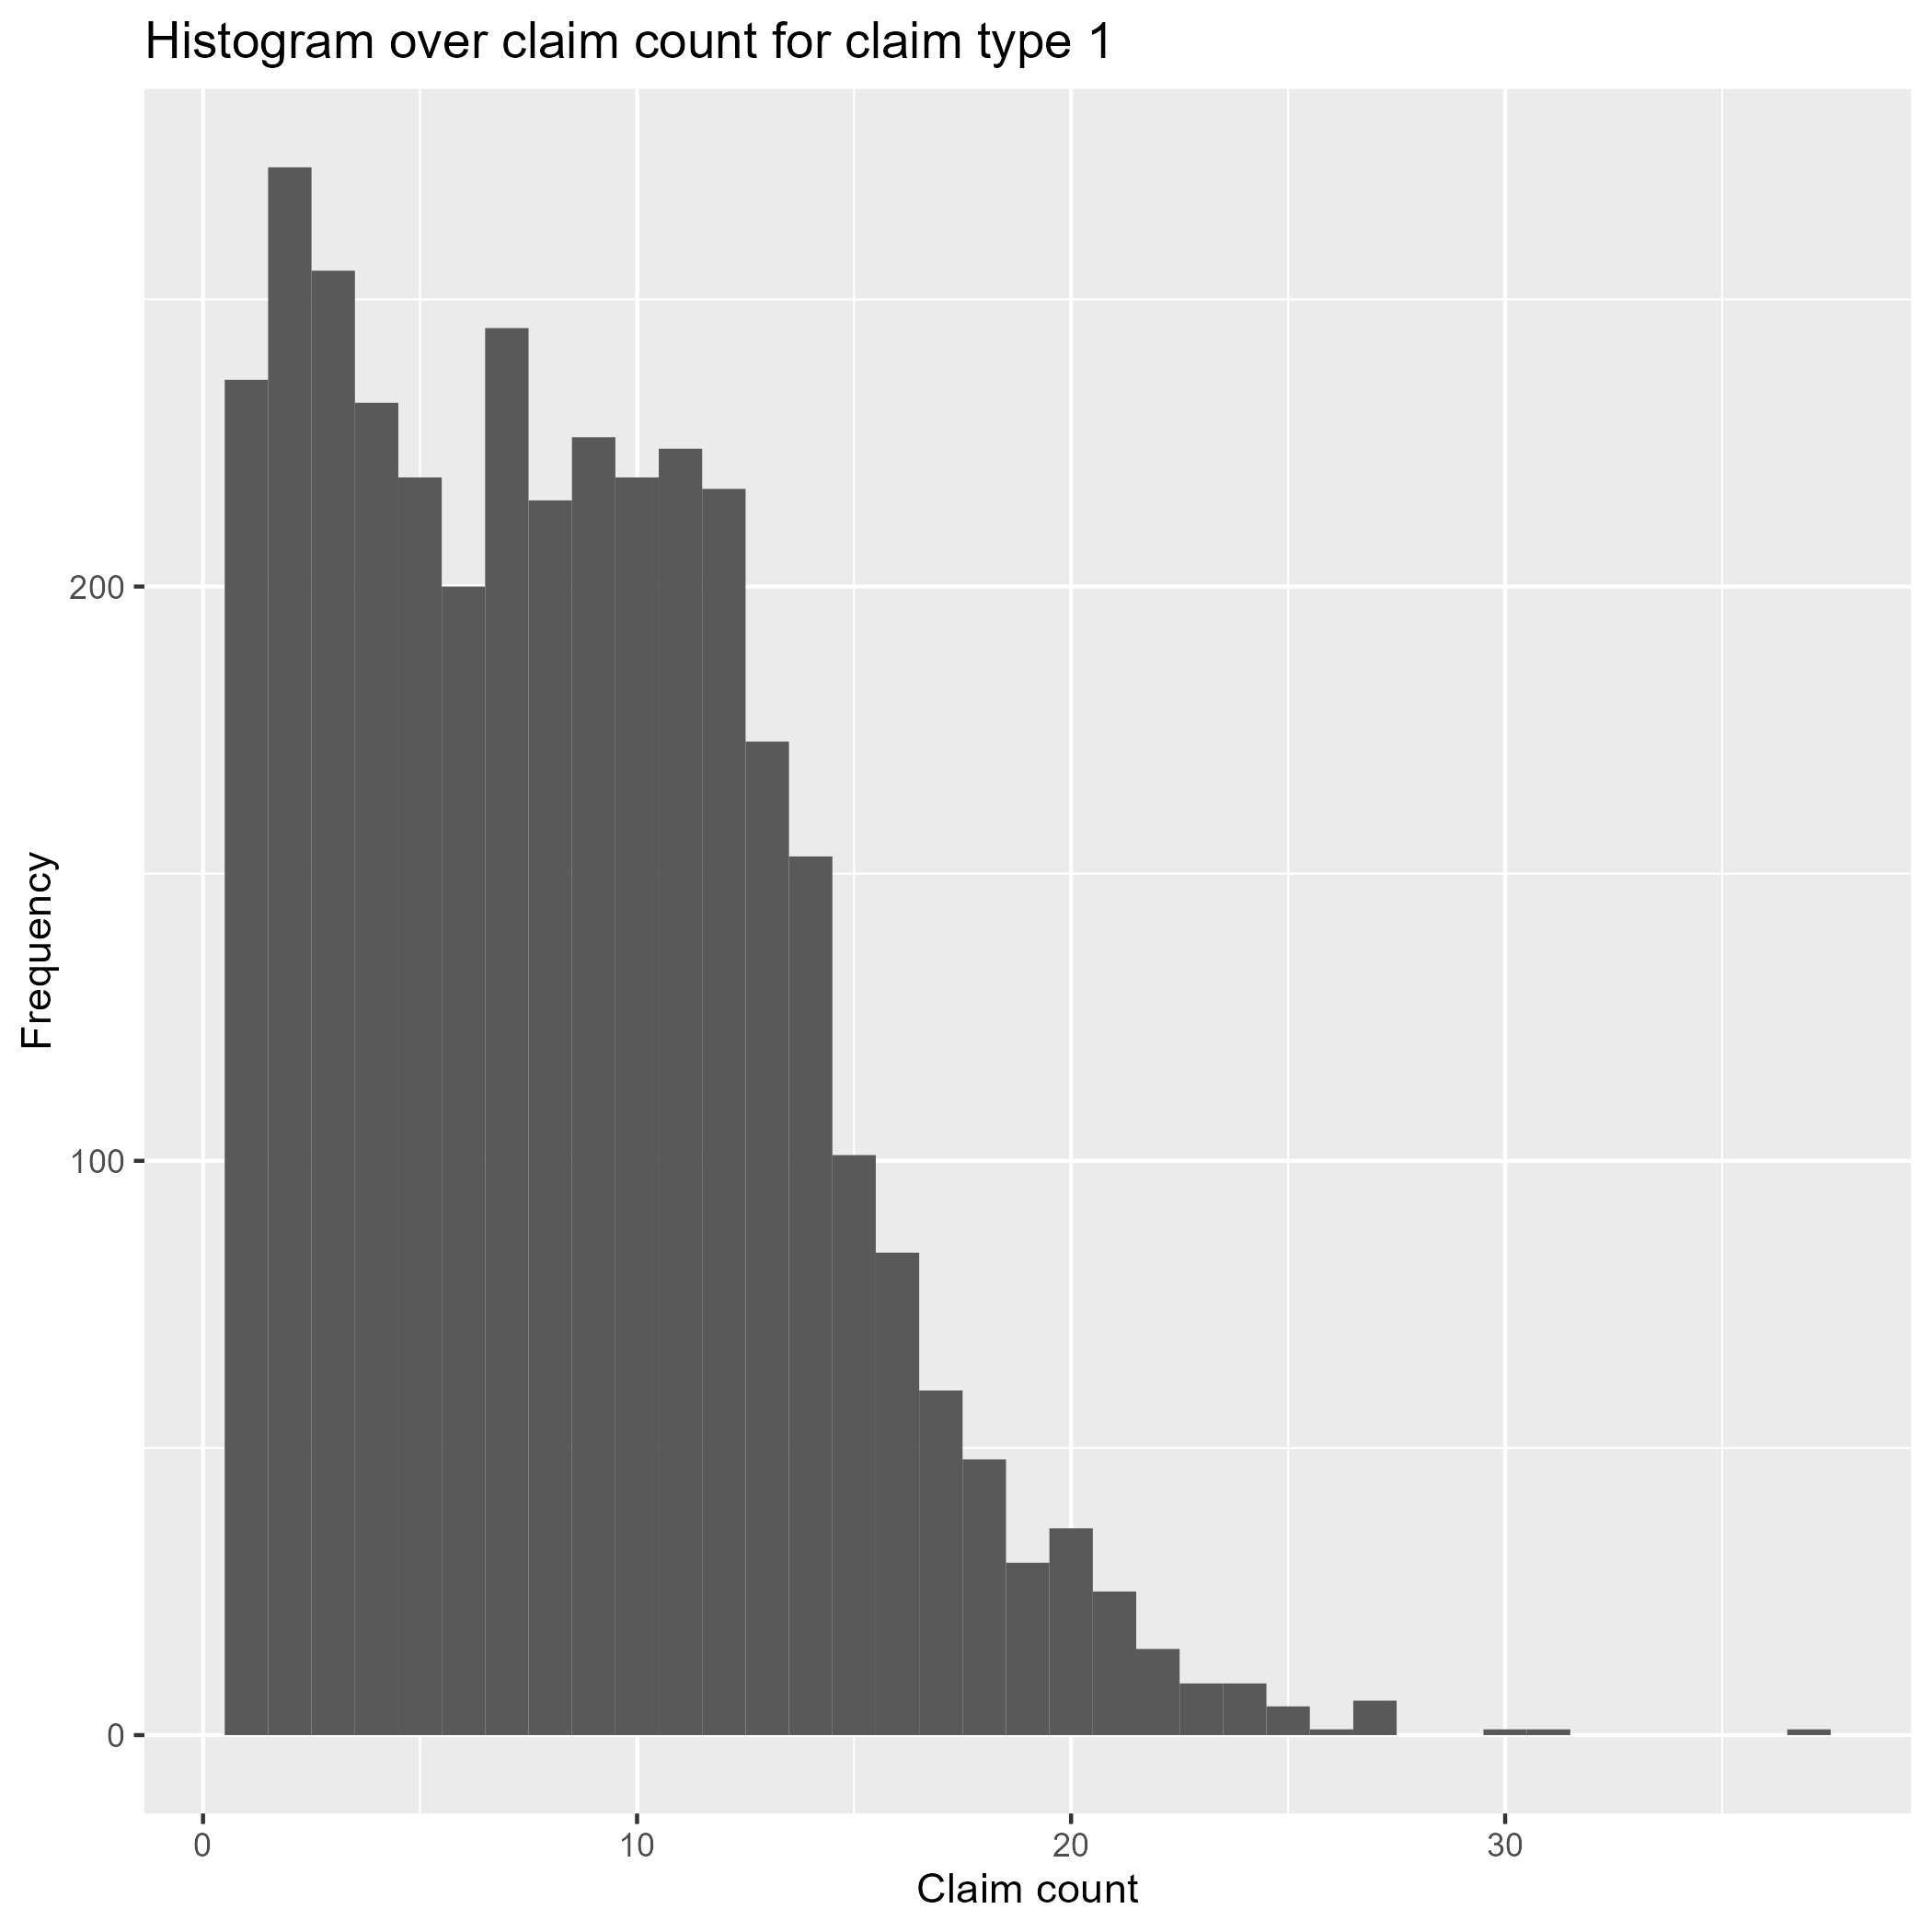
\includegraphics[width=.6\linewidth]{plots/simulation/histogram_claim_count1.png}
        \caption{Branch 1.}
    \end{subfigure}
    \begin{subfigure}{.49\textwidth}
        \centering
        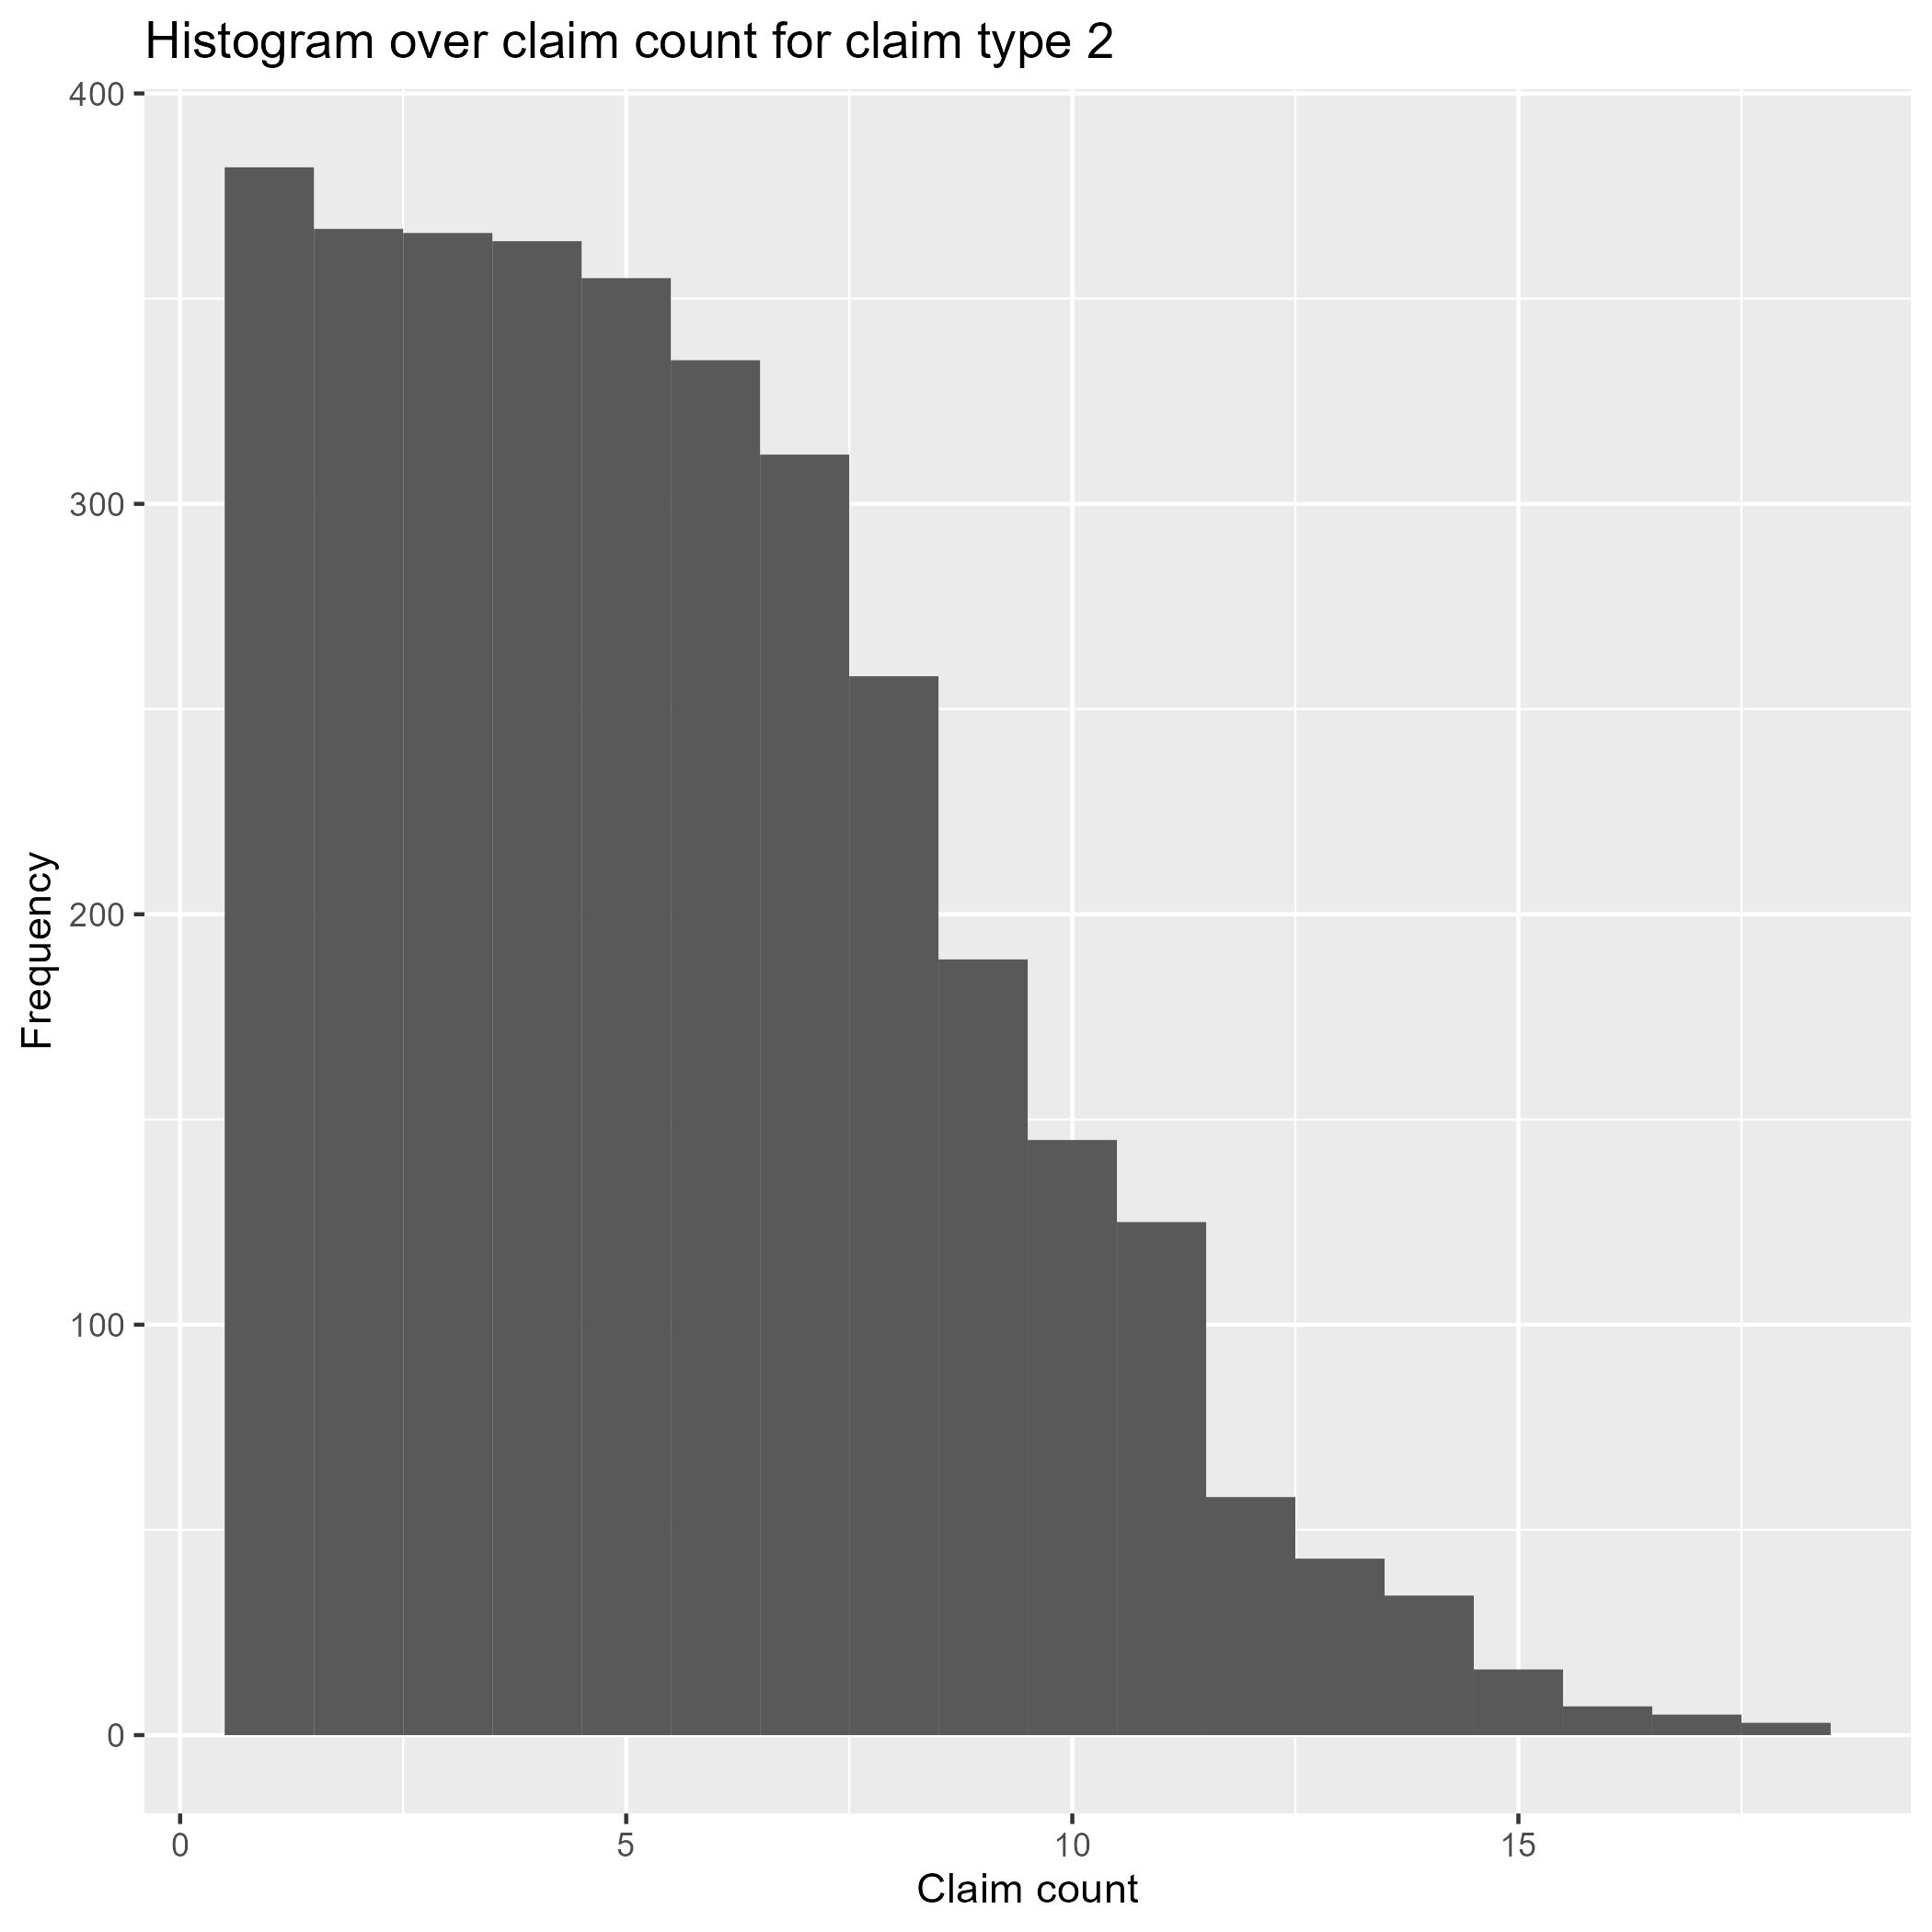
\includegraphics[width=.6\linewidth]{plots/simulation/histogram_claim_count2.png}
        \caption{Branch 2.}
    \end{subfigure}
    \label{a4:claimcount}
    \caption{Simulated amount of claims in both branches respectively.}
\end{figure}

Simulating the claim cost a 1000 times, simulating 10 years each time we end up on the distributions in figure \ref{a4:claim_cost1}.
As seen the simulated amounts resemble and distributes around the observed amount, implying that our simulation works correctly.
Also observe the law of large number becoming apparent, as the sum of many random variables converges towards a normal distribution.

\begin{figure}[!h]
\centering
    \begin{subfigure}{.24\textwidth}
      \centering
      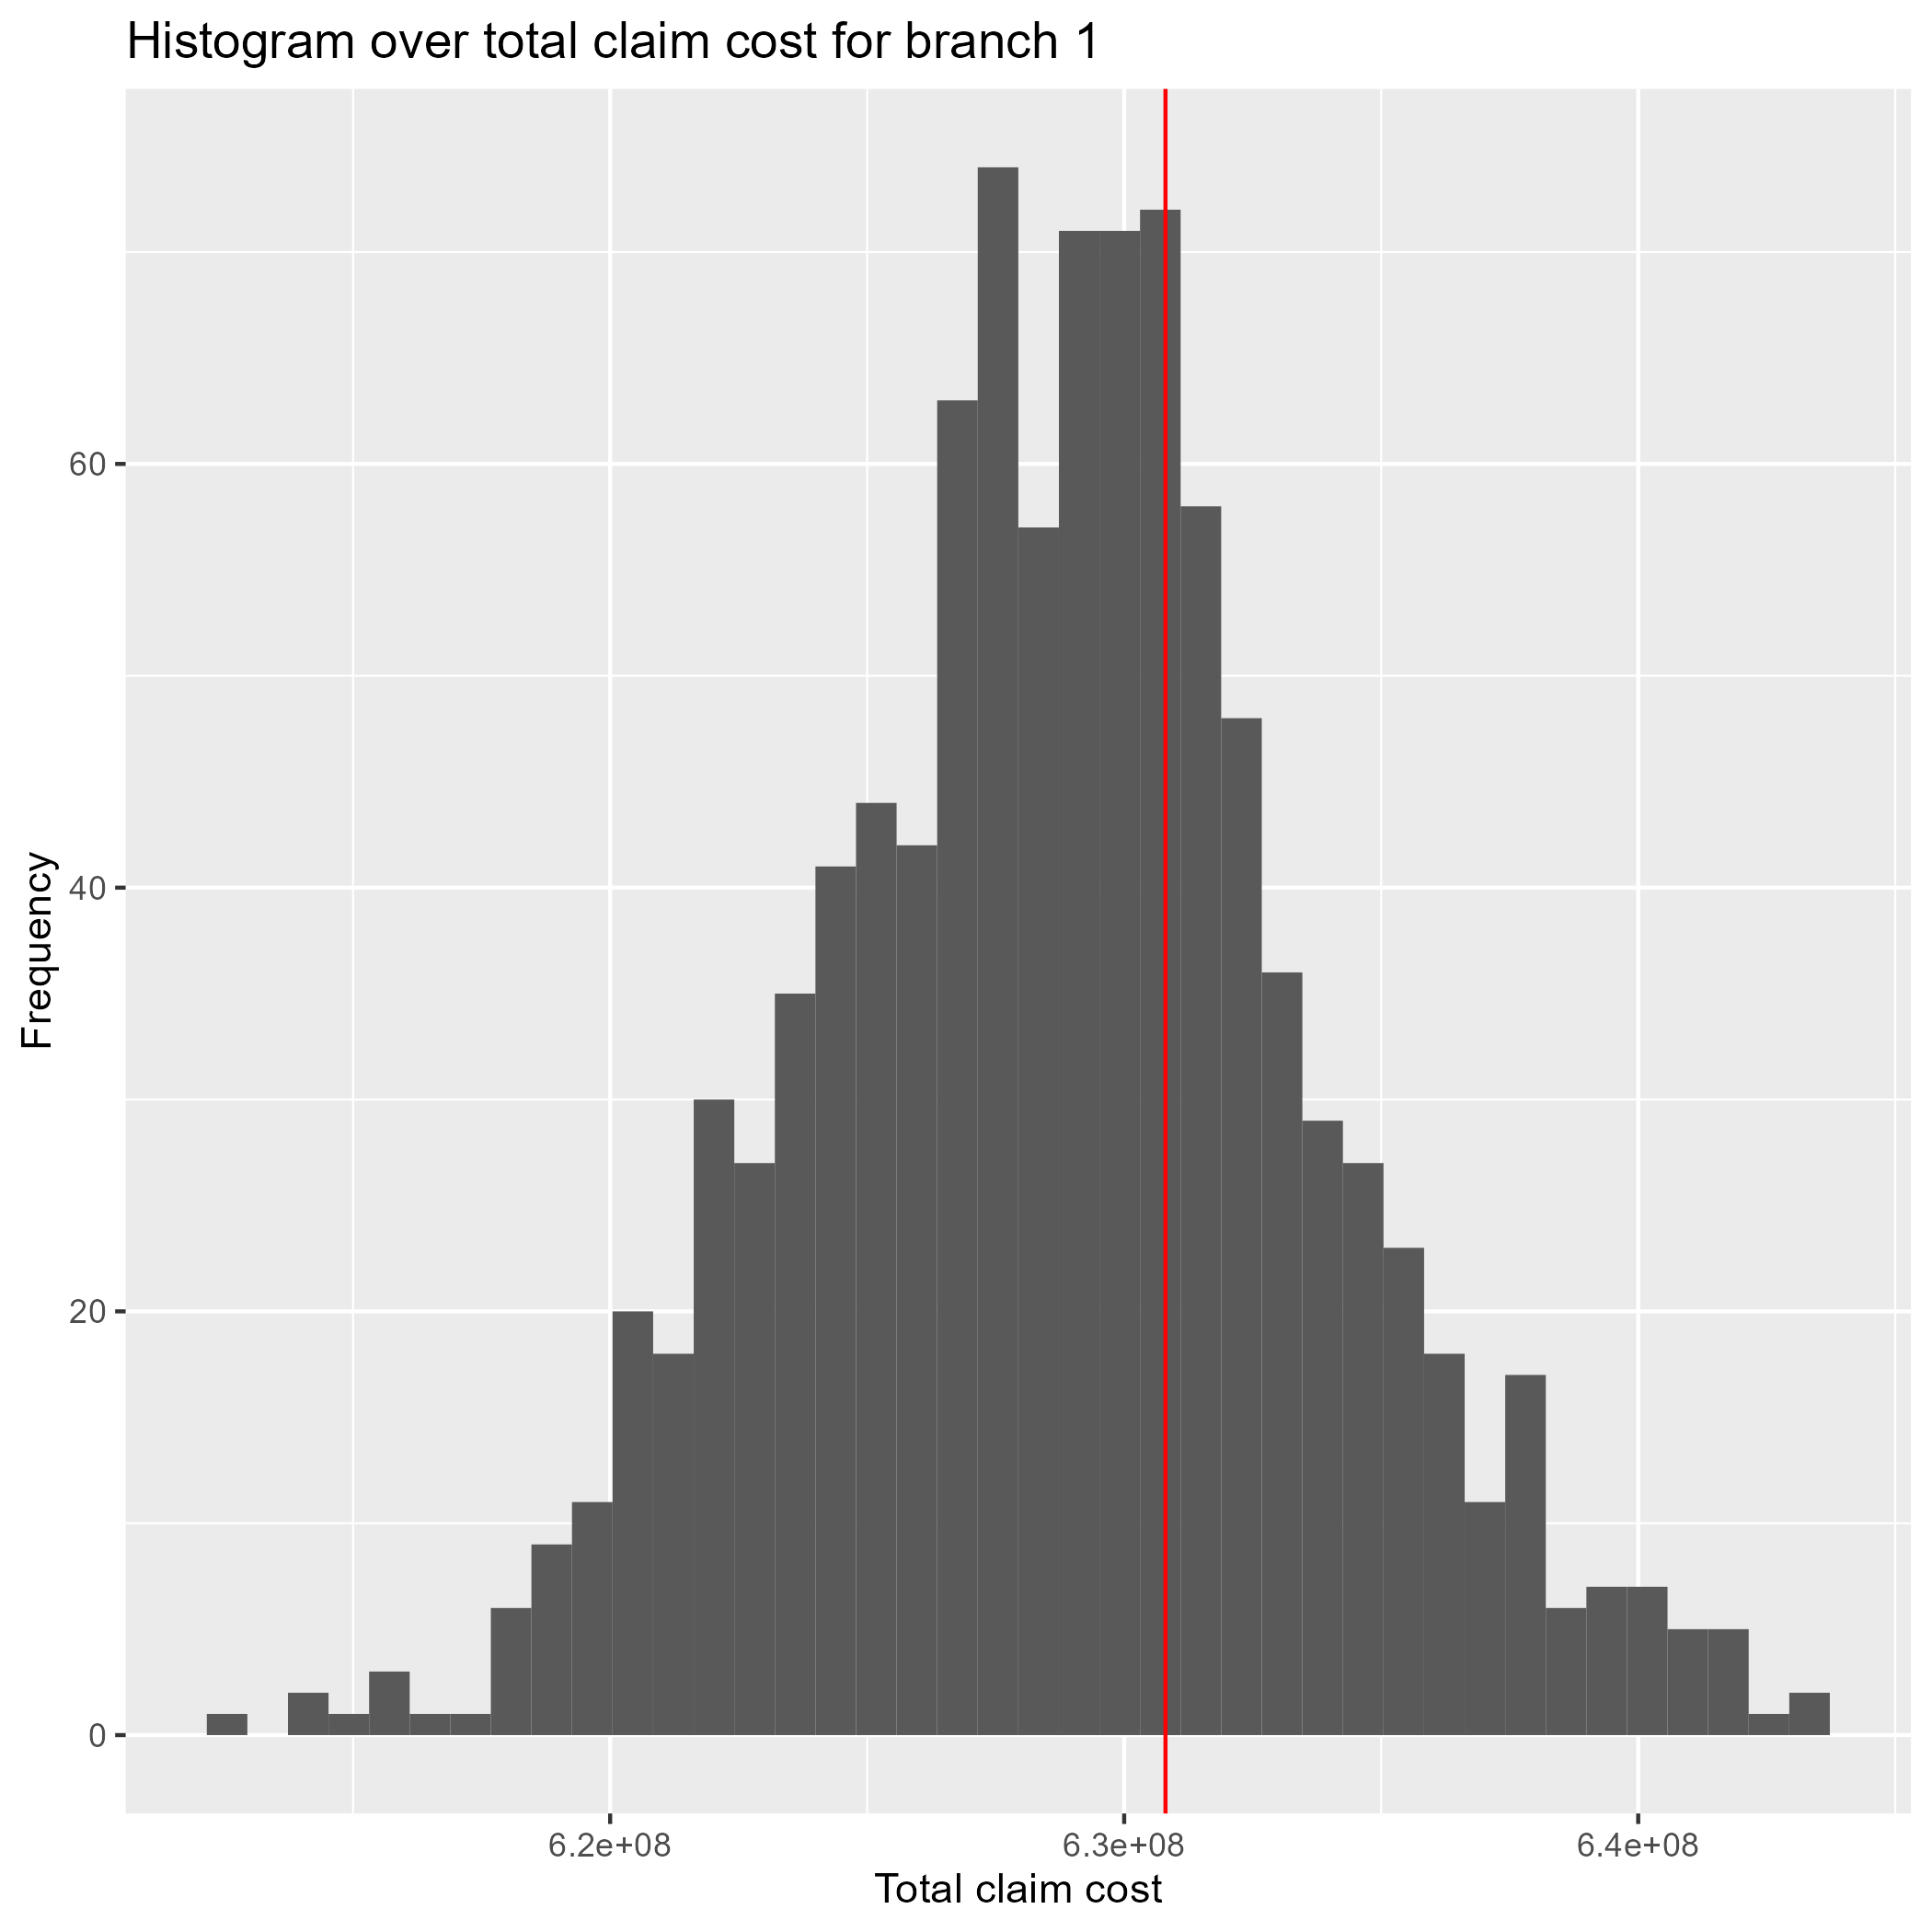
\includegraphics[width=.9\linewidth]{plots/simulation/histogram_total_claim_cost_small1.png}
      \caption{Branch 1 Small.}
    \end{subfigure}%
    \begin{subfigure}{.24\textwidth}
      \centering
      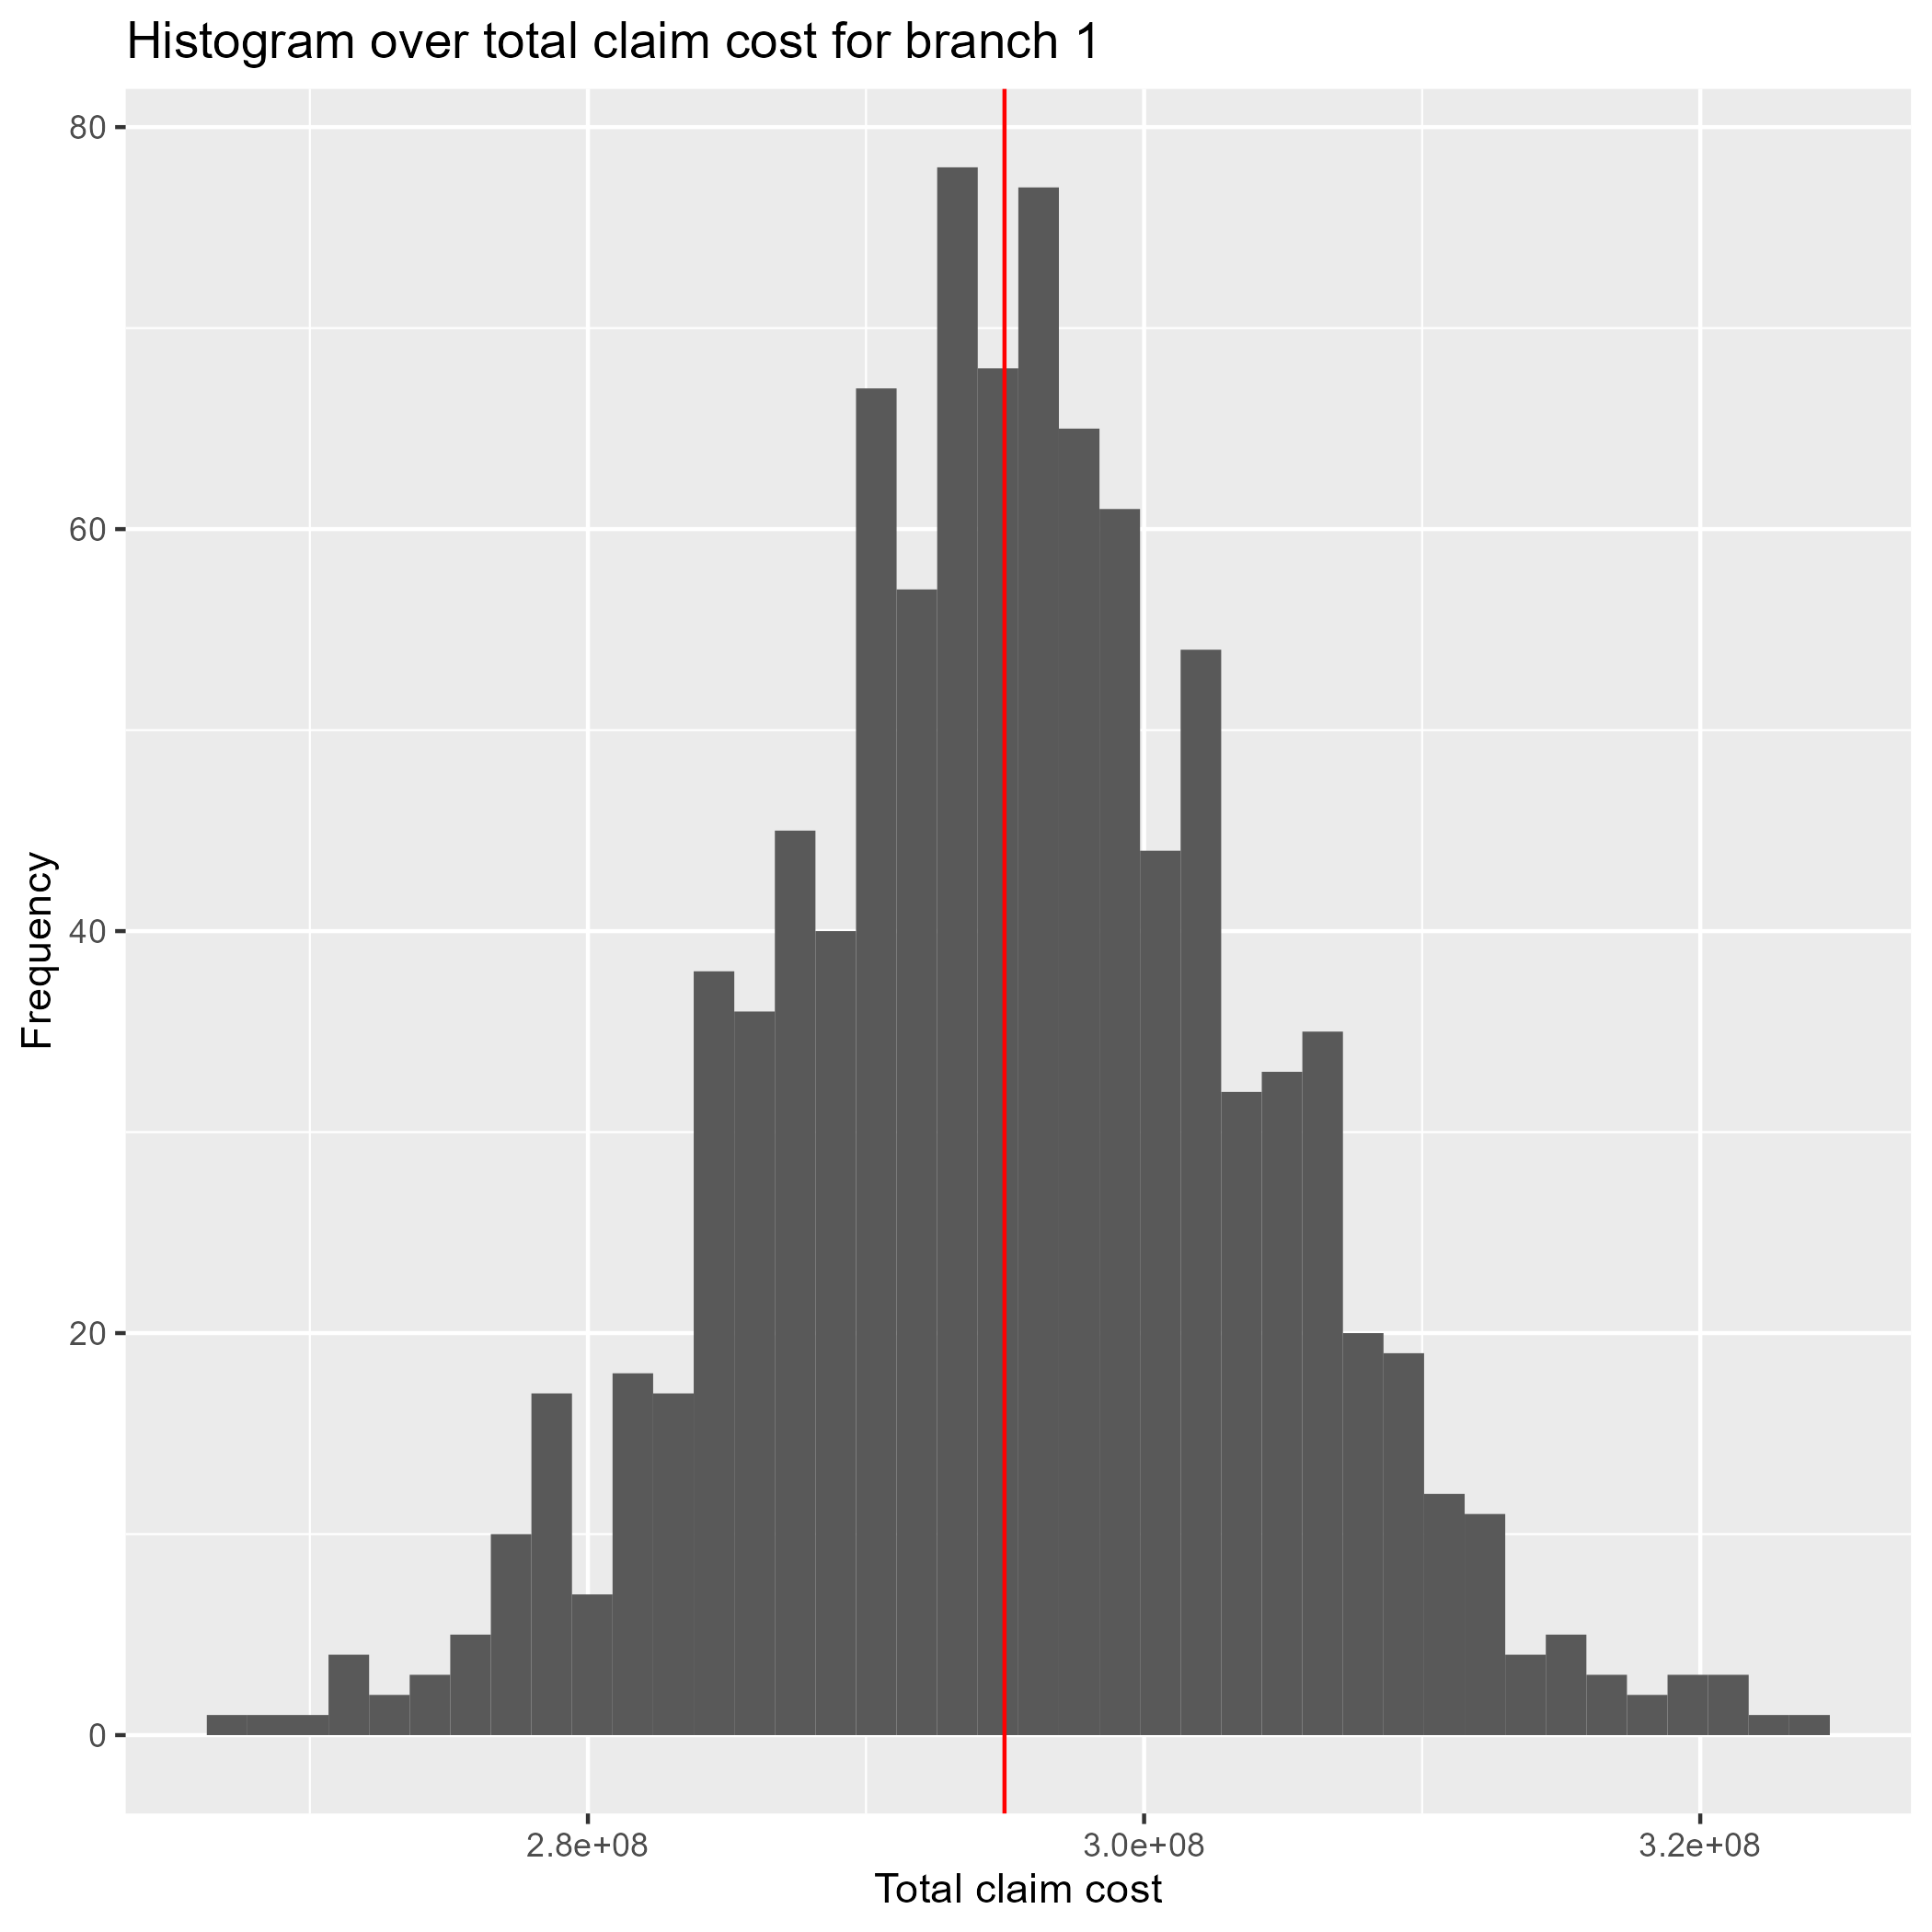
\includegraphics[width=.9\linewidth]{plots/simulation/histogram_total_claim_cost_large1.png}
      \caption{Branch 1 Large.}
    \end{subfigure}
    \begin{subfigure}{.24\textwidth}
      \centering
      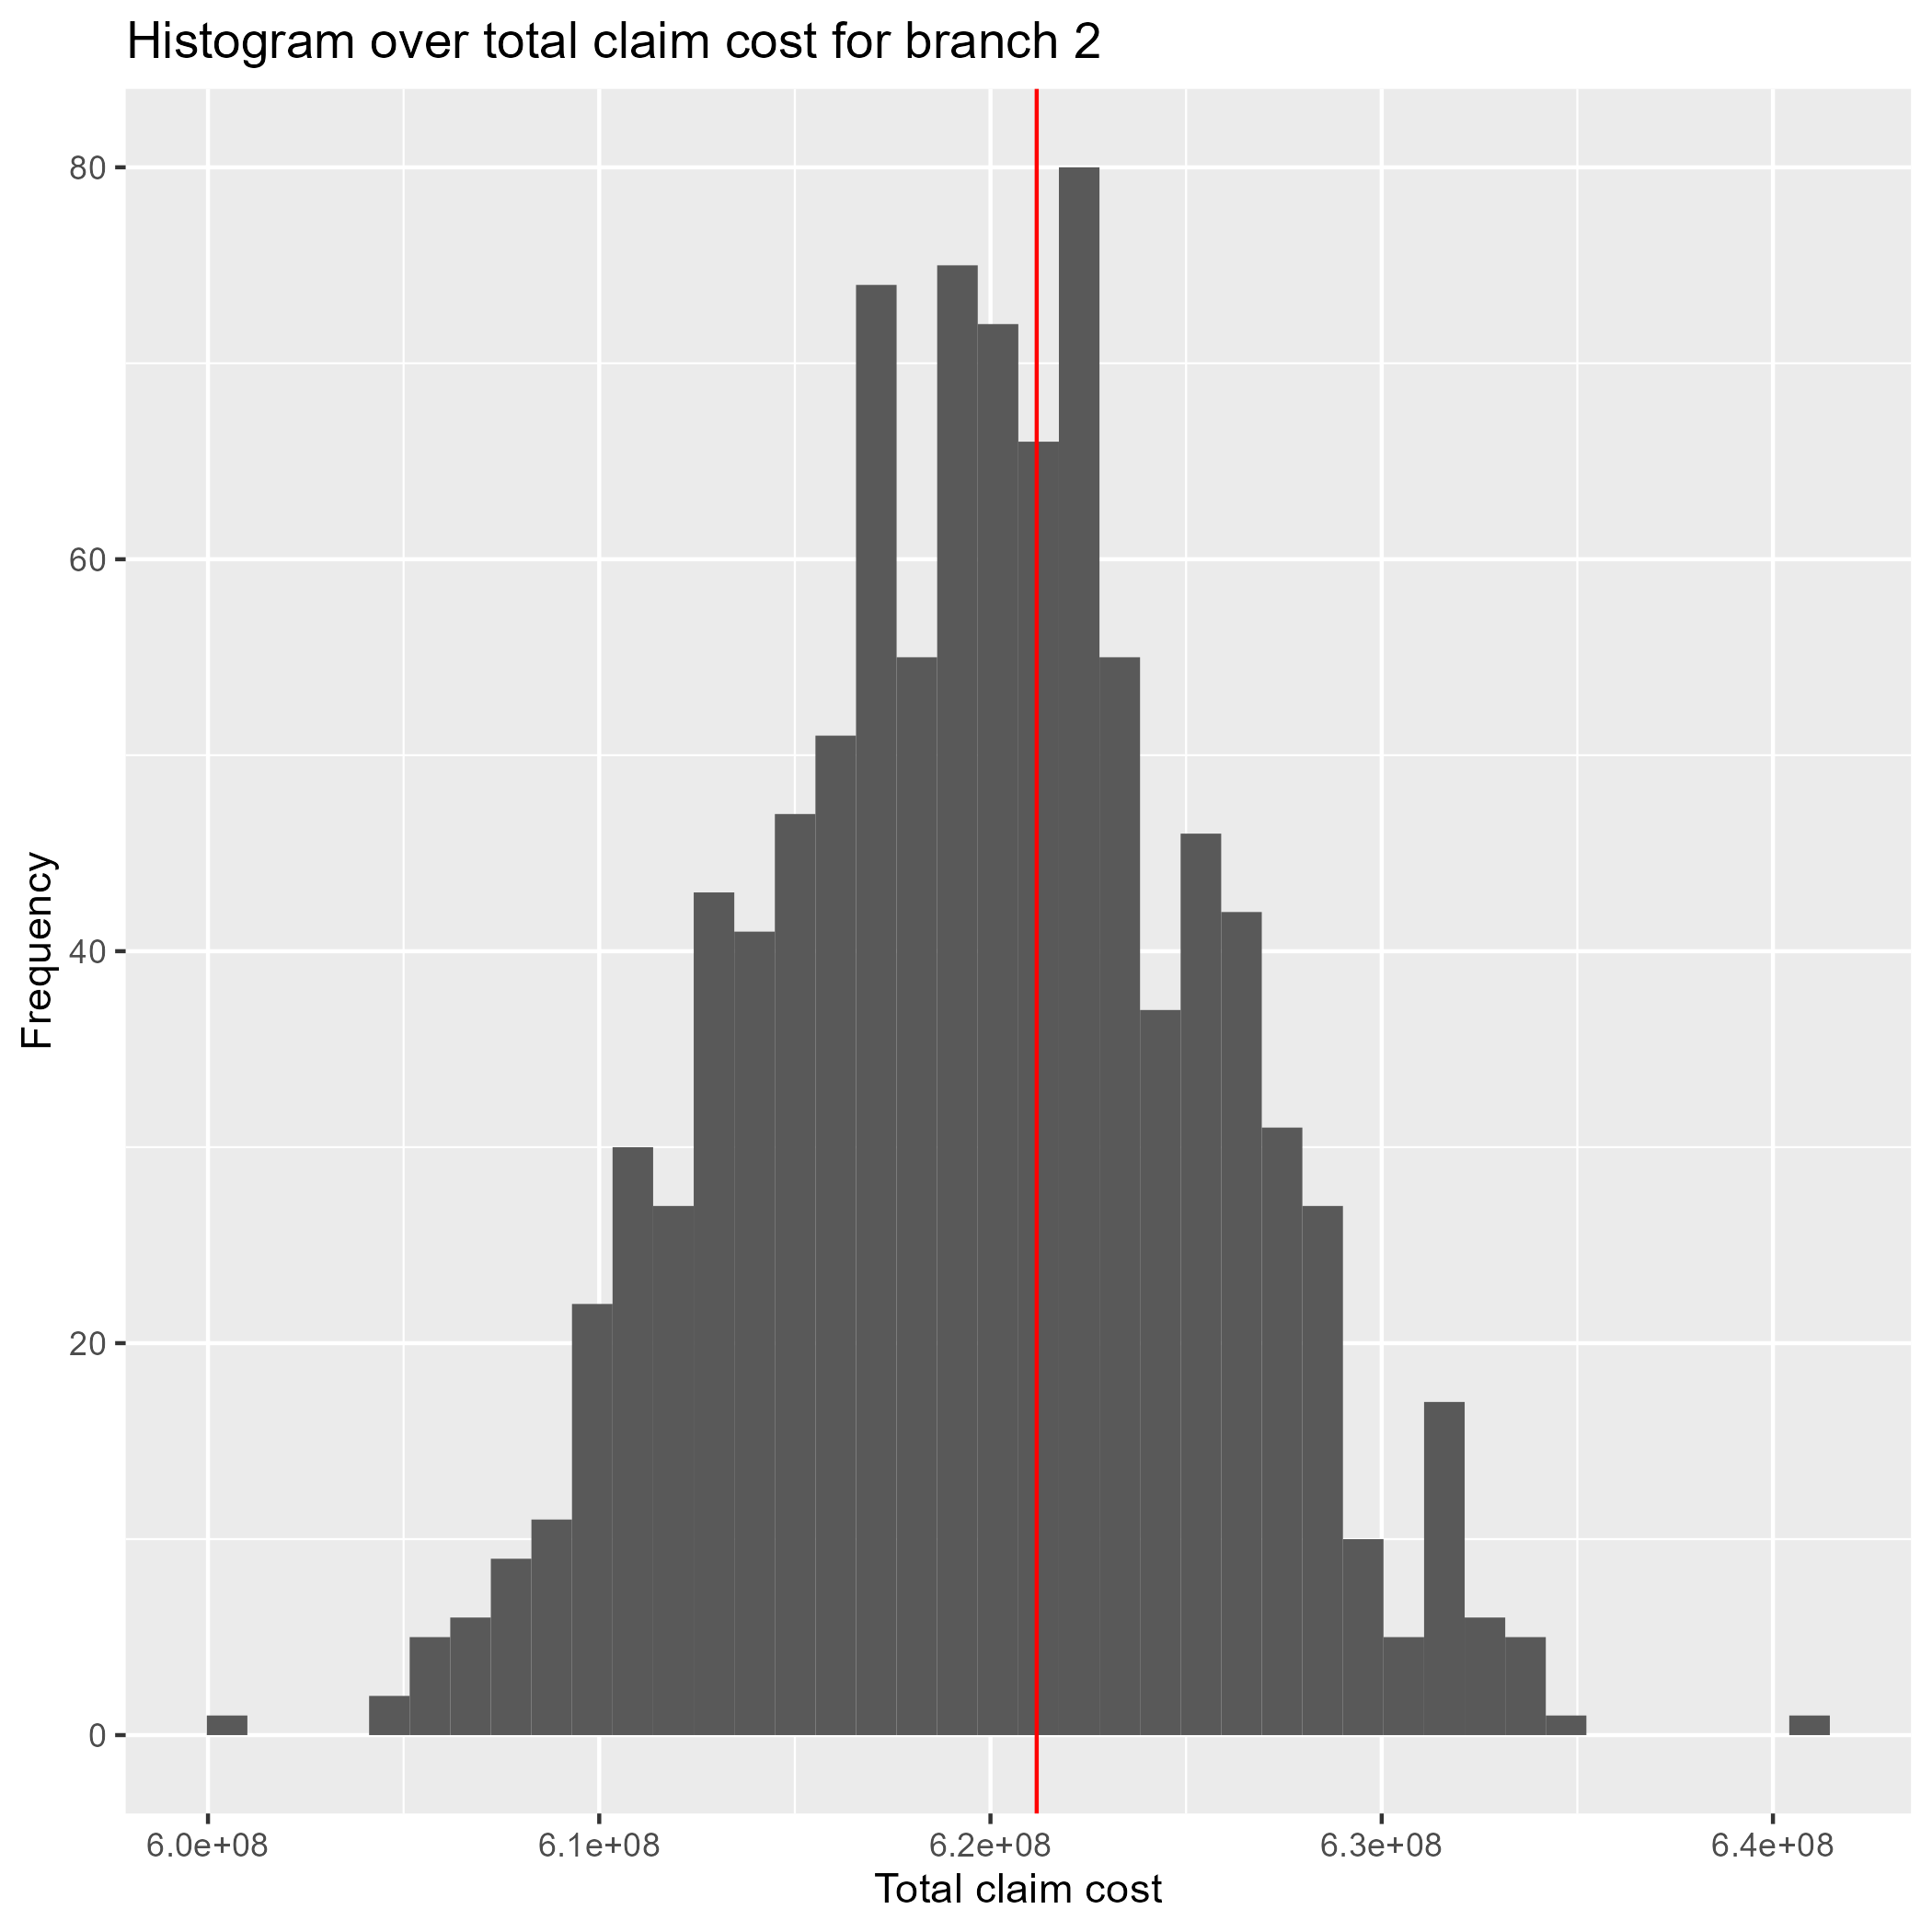
\includegraphics[width=.9\linewidth]{plots/simulation/histogram_total_claim_cost_small2.png}
      \caption{Branch 2 Small.}
    \end{subfigure}%
    \begin{subfigure}{.24\textwidth}
      \centering
      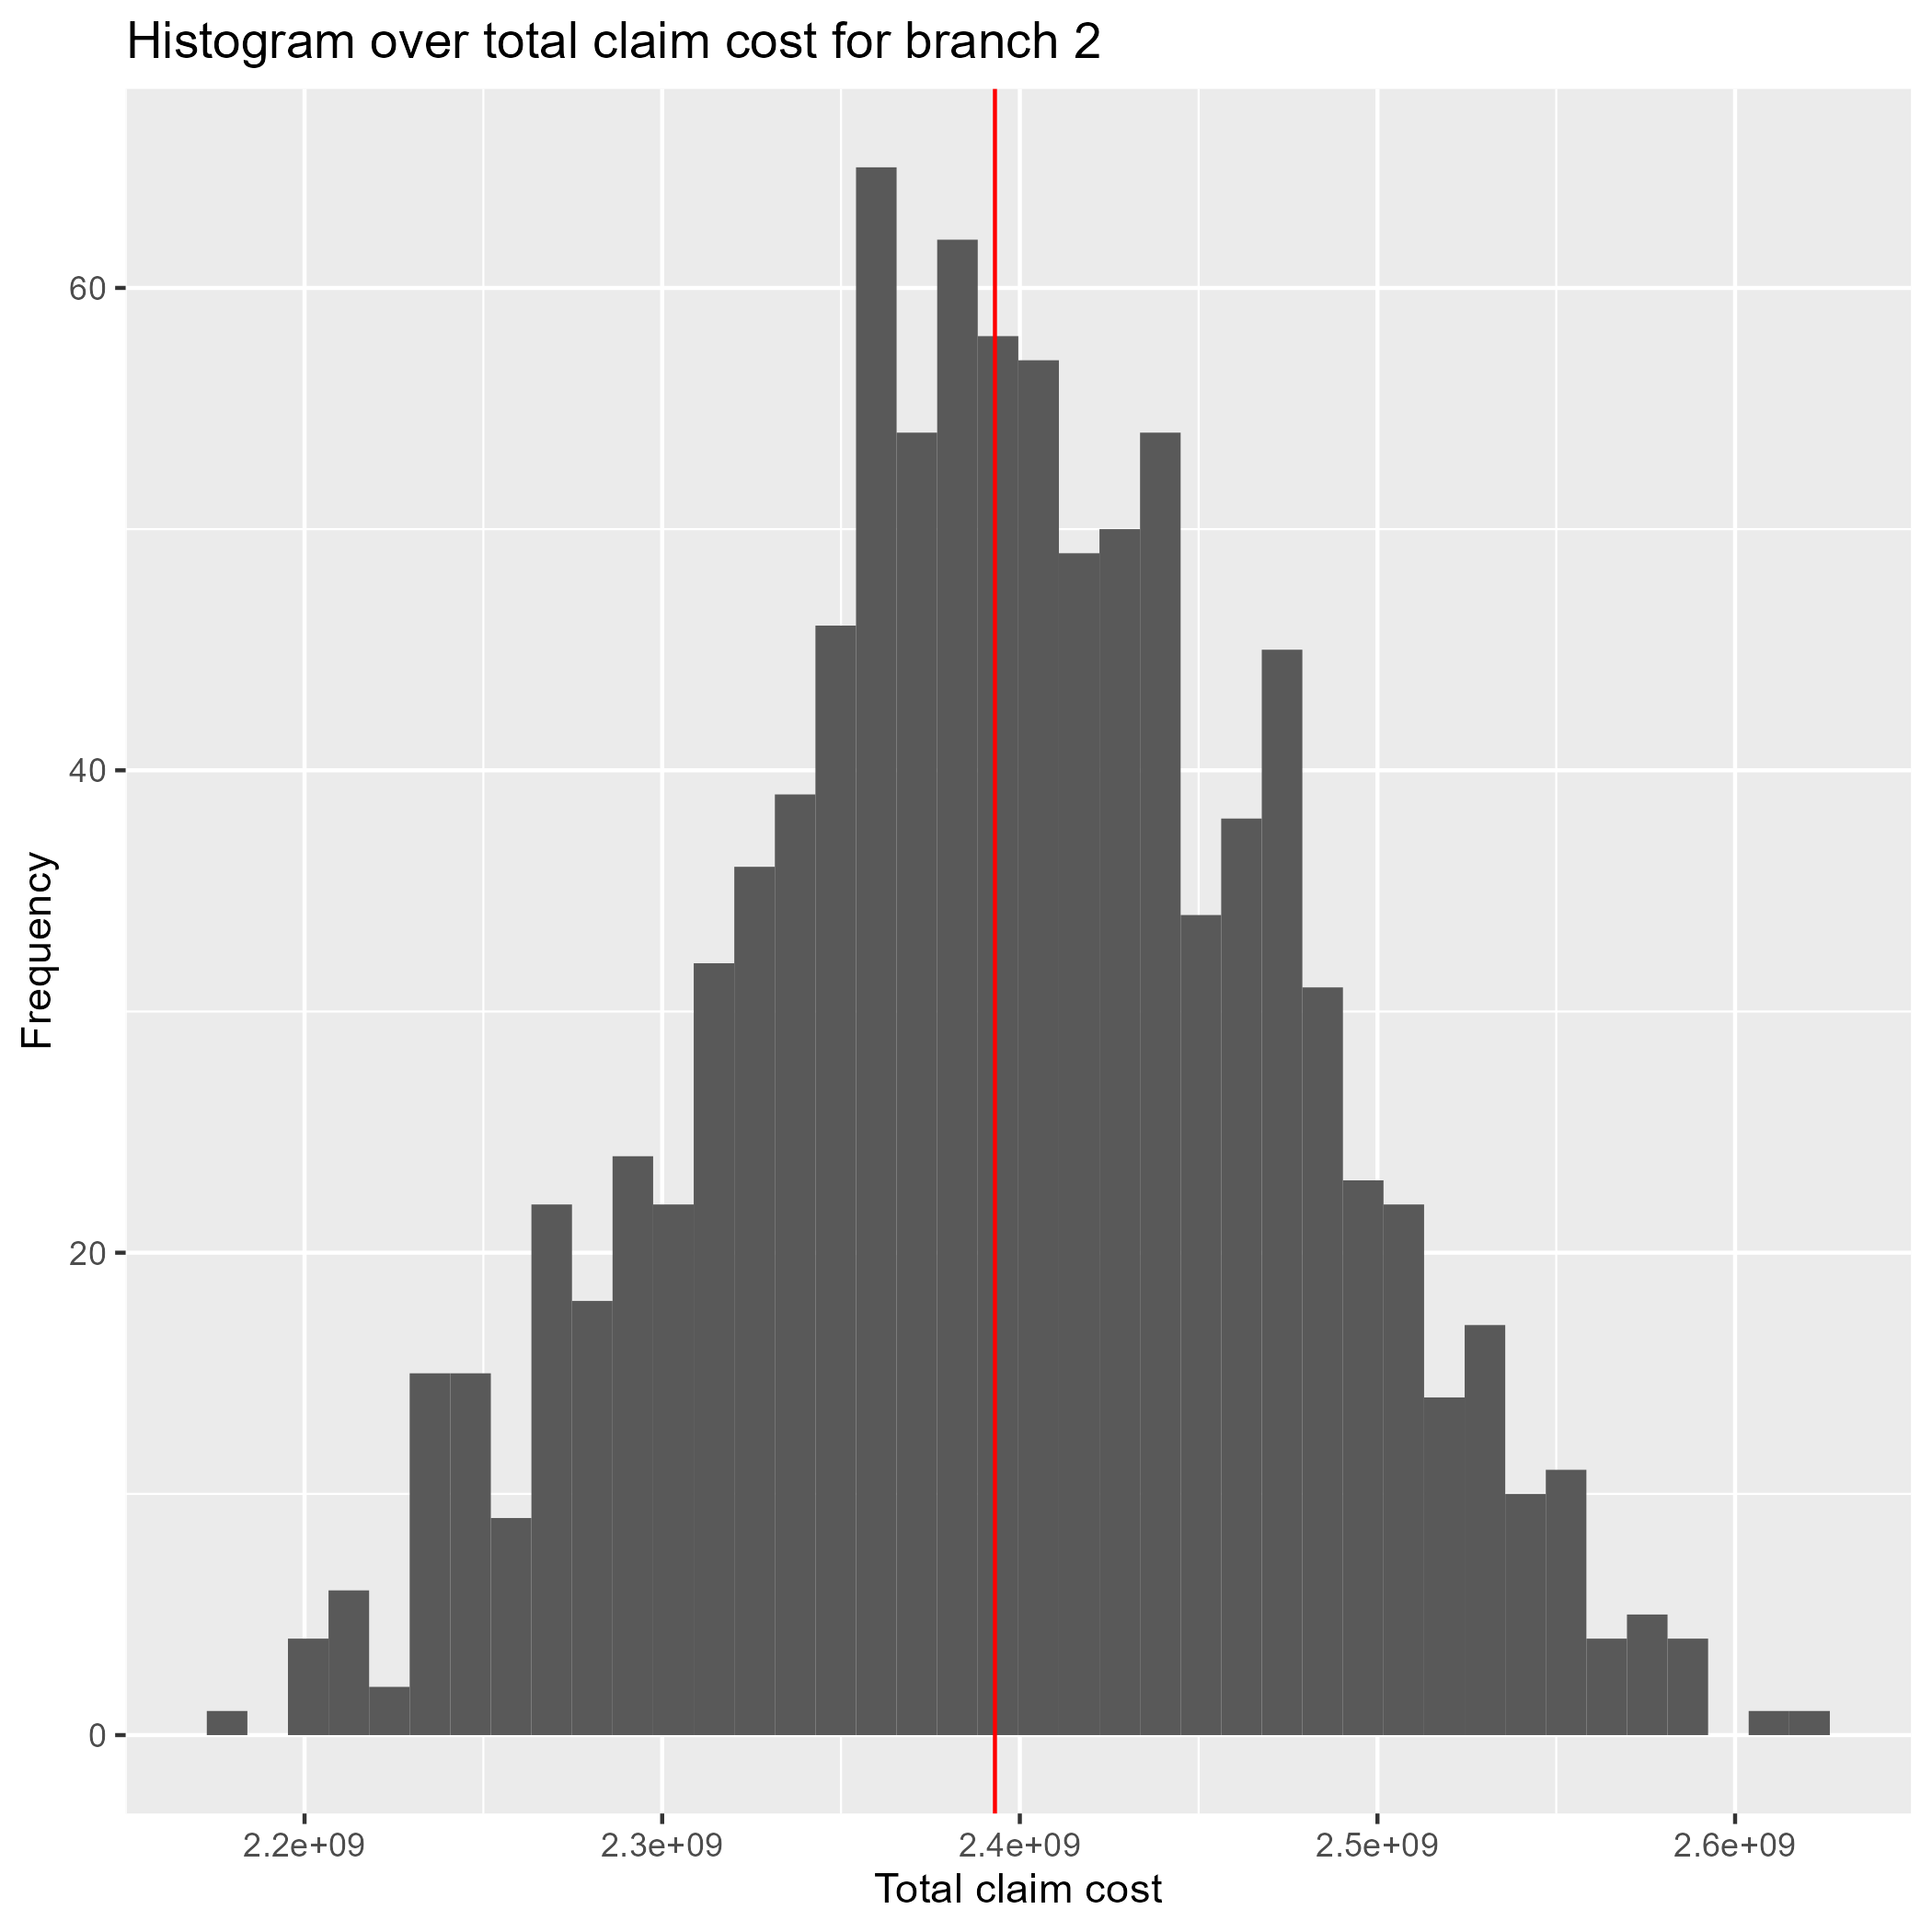
\includegraphics[width=.9\linewidth]{plots/simulation/histogram_total_claim_cost_large2.png}
      \caption{Branch 2 Large.}
    \end{subfigure}
    \caption{Simulated claim amounts compared to observed value in red.}
    \label{a4:claim_cost1}
\end{figure}

To conclude the chapter on the simulations we study the total cost as a final sanity check.
As observed in figure \ref{a4:claim_cost2}, the total amounts also distributes nicely around the observed amount.
We also observe the law of large numbers being apparent here as well, and get indications of the final claim costs.

 \begin{figure}[!h]
\centering
    \begin{subfigure}{.33\textwidth}
      \centering
      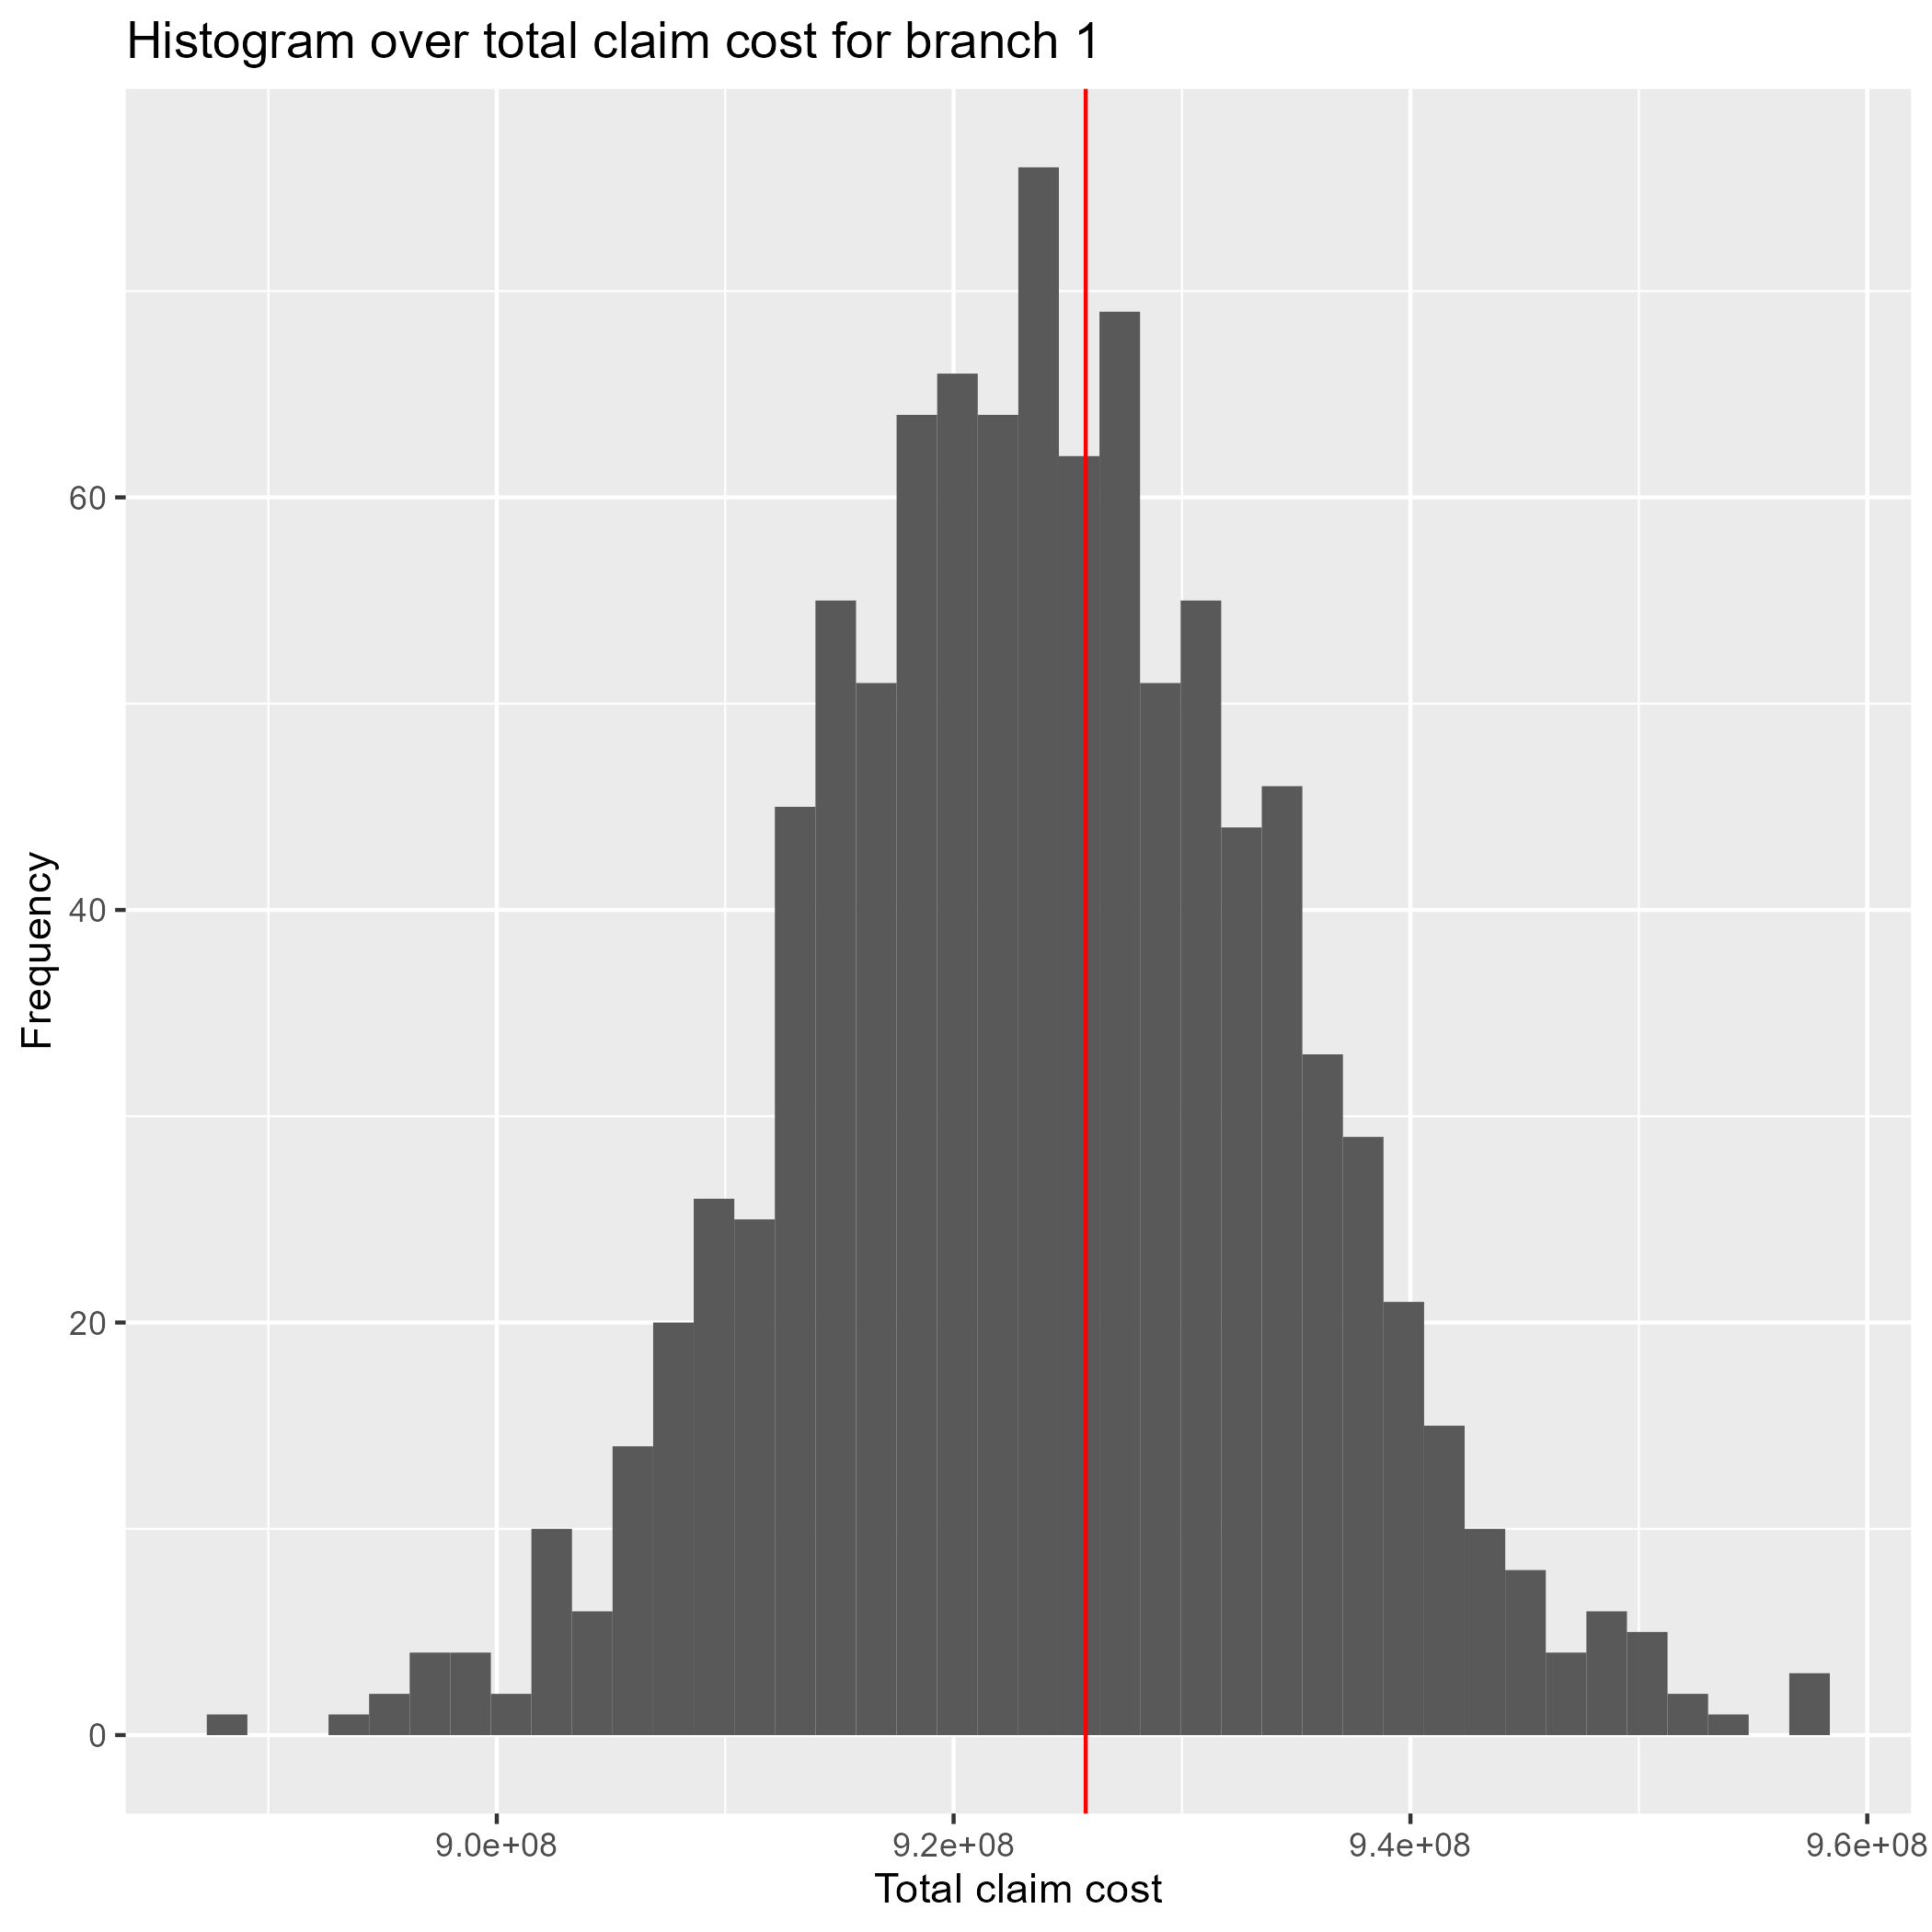
\includegraphics[width=.9\linewidth]{plots/simulation/histogram_total_claim_cost1.png}
      \caption{Branch 1 Claims.}
    \end{subfigure}%
    \begin{subfigure}{.33\textwidth}
      \centering
      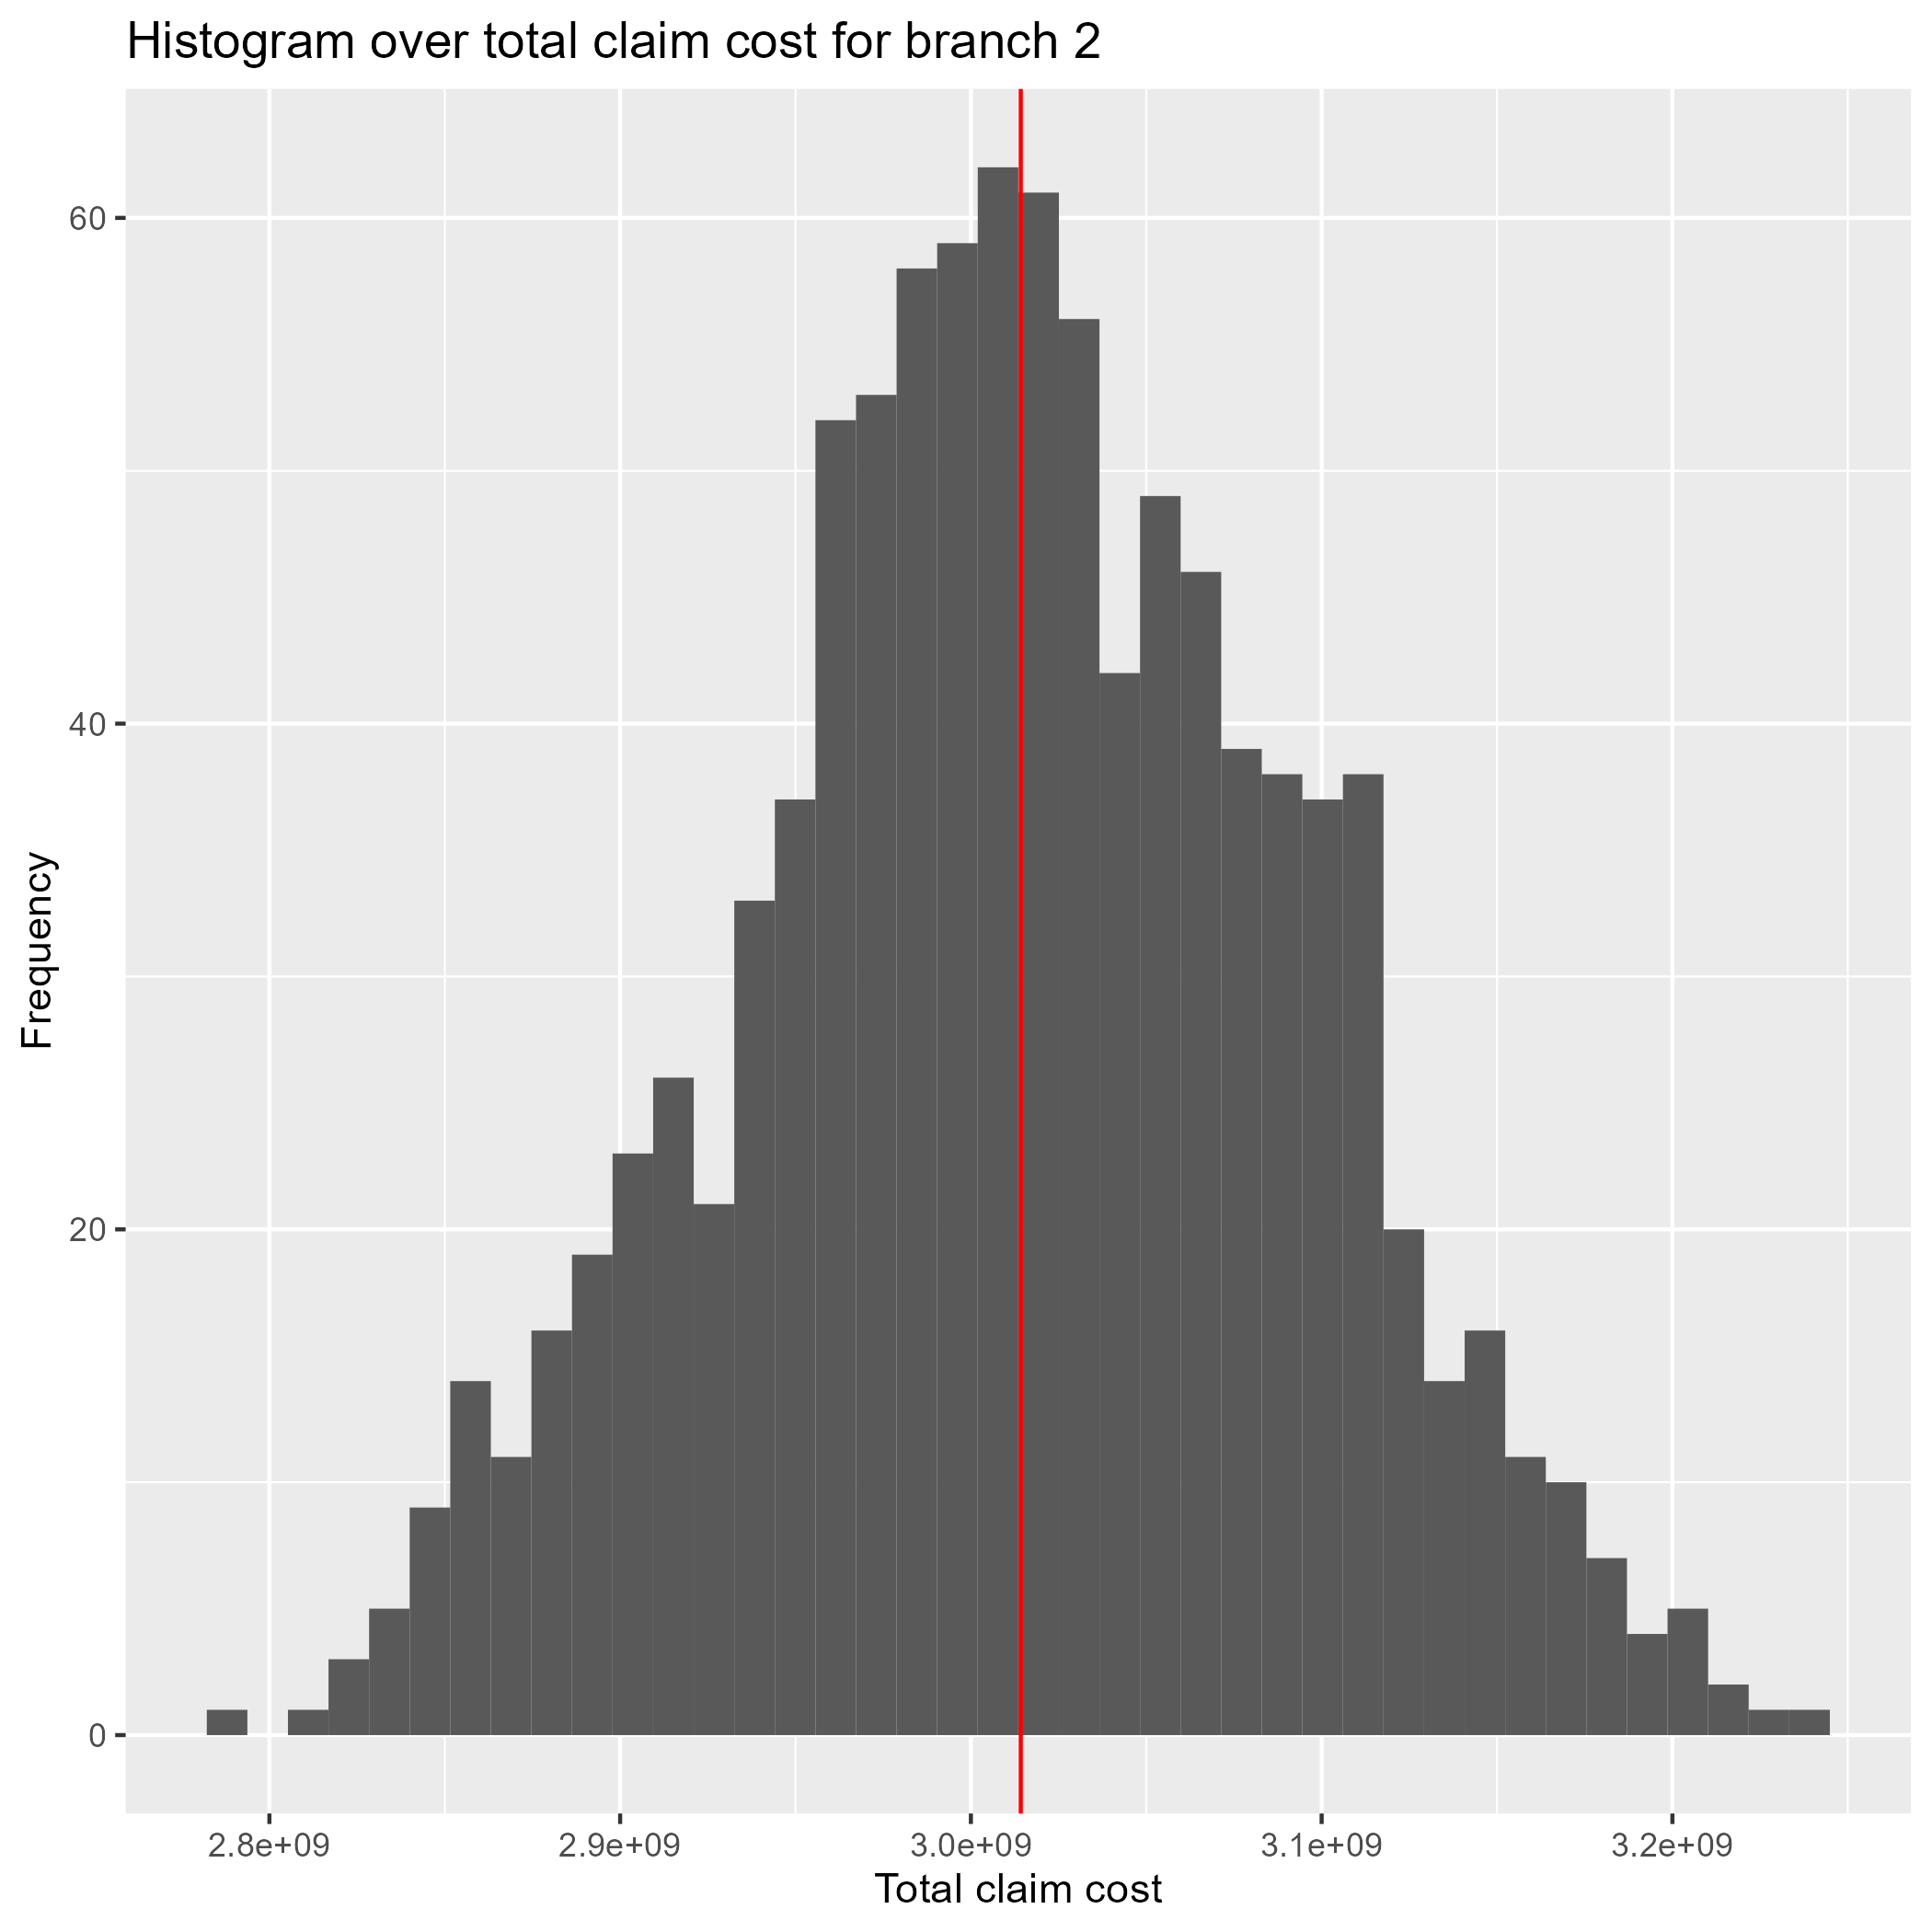
\includegraphics[width=.9\linewidth]{plots/simulation/histogram_total_claim_cost2.png}
      \caption{Branch 2 Claims.}
    \end{subfigure}
    \begin{subfigure}{.33\textwidth}
      \centering
      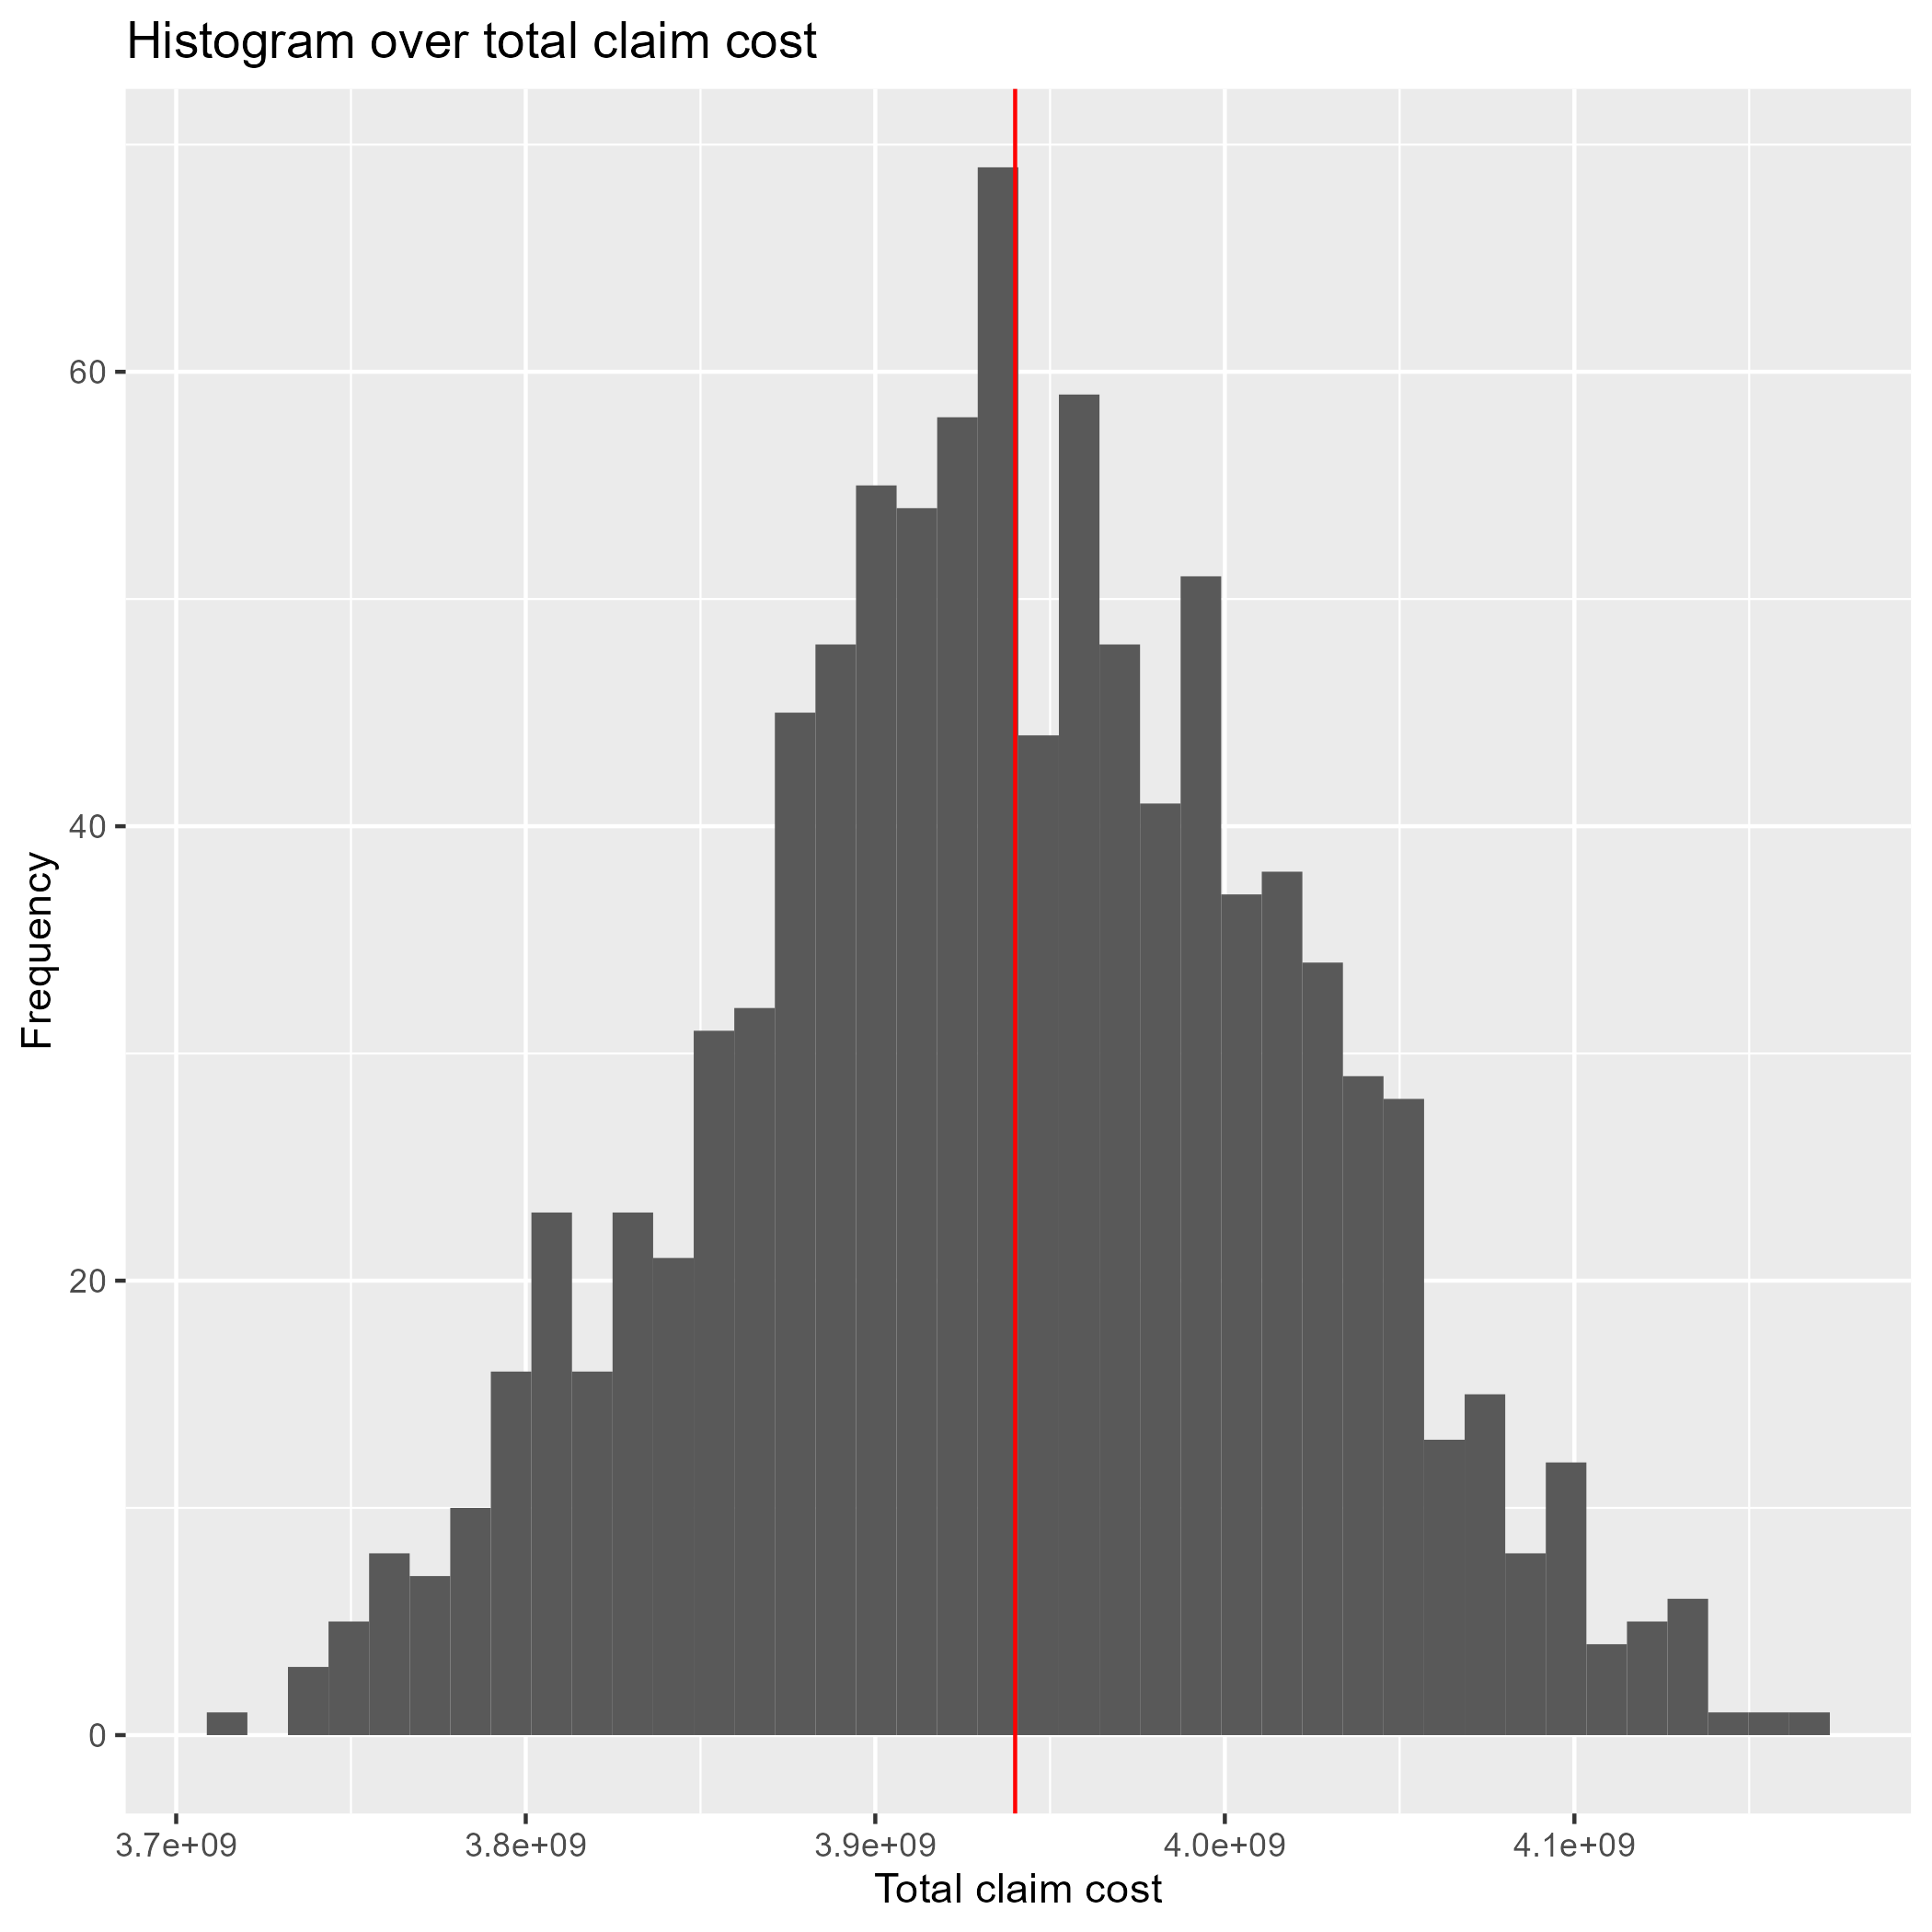
\includegraphics[width=.9\linewidth]{plots/simulation/histogram_total_claim_cost.png}
      \caption{Total Claims.}
    \end{subfigure}%
    \caption{Simulated total claim amounts compared to observed value in red.}
    \label{a4:claim_cost2}
\end{figure}

\subsection*{Working with Reinsurance}
The next 3 questions regard applying reinsurance products on top of our claim data.
We will study 3 different reinsurance product and evaluate the scenarios the product is profitable, and how it affects our total claim costs as an insurance company.

A common method through these 3 sections is that to estimation of quantiles and the reinsurance expected cost which will be evaluated using  simulated data using algorithm in \ref{a4:alg}.
One could derive an analytical solution for the given probability distributions model we have used, but due to simplicity, and according to how one usually estimates these costs in practice, we used the simulation tools.
Do observe that we will simulate the claim outcomes from a seperate simulation, not being the one which we esstimate the quantiles and reinsurance cost on.

\subsubsection*{The XL Cover}

Applying the XL cover, we simulated 100 runs to estimate the 90\% quantile of the data, and estimated the total cost exceeding this quantile in each run.
As a result, seen in figure \ref{a5:simulation}, which shows how the quantile shows some law of large numbers normality.
Also observe that the insurance claims have a clear cutoff-point around the estimated mean when simulating a years claims.
Also observe that the claim cost of branch 1 are more uniform compared to barnch 2, which have a larger distinguishing between large and small claims.

 \begin{figure}[!h]
\centering
    \begin{subfigure}{.24\textwidth}
      \centering
      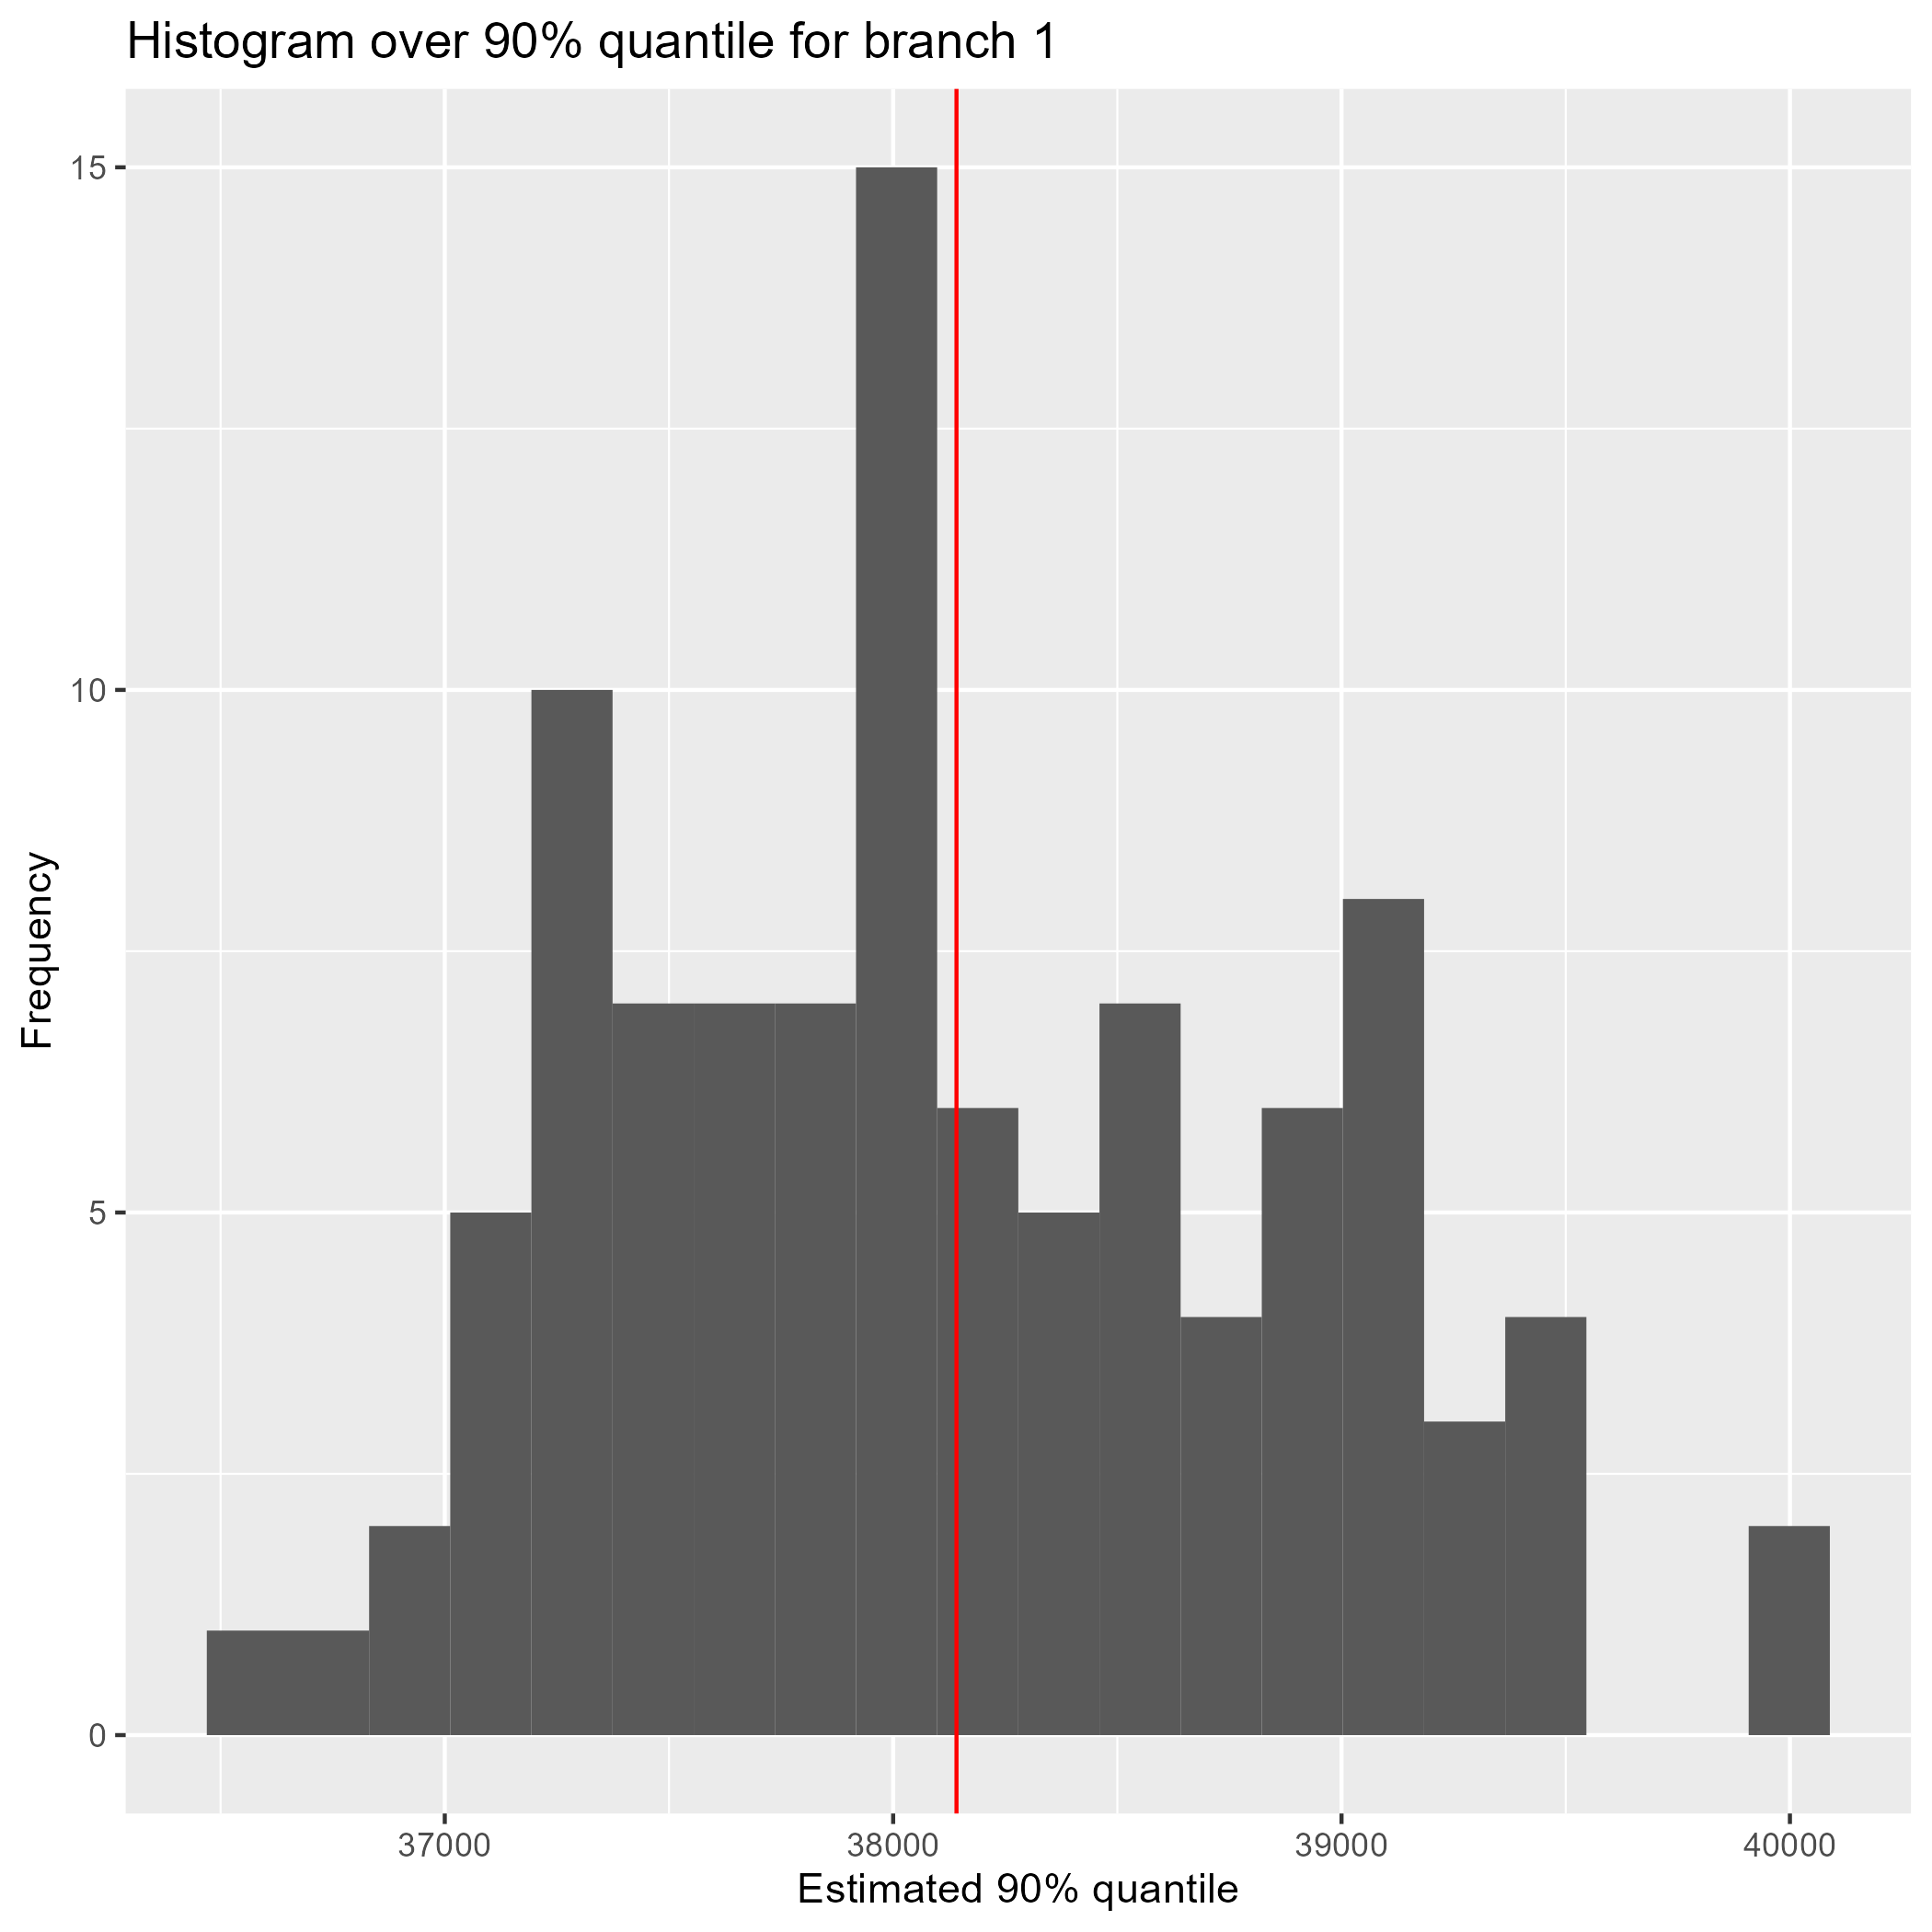
\includegraphics[width=.9\linewidth]{plots/reinsurance1/histogram_over_90p_quantile_1.png}
      \caption{Branch 1 Quantile.}
    \end{subfigure}
    \begin{subfigure}{.24\textwidth}
      \centering
      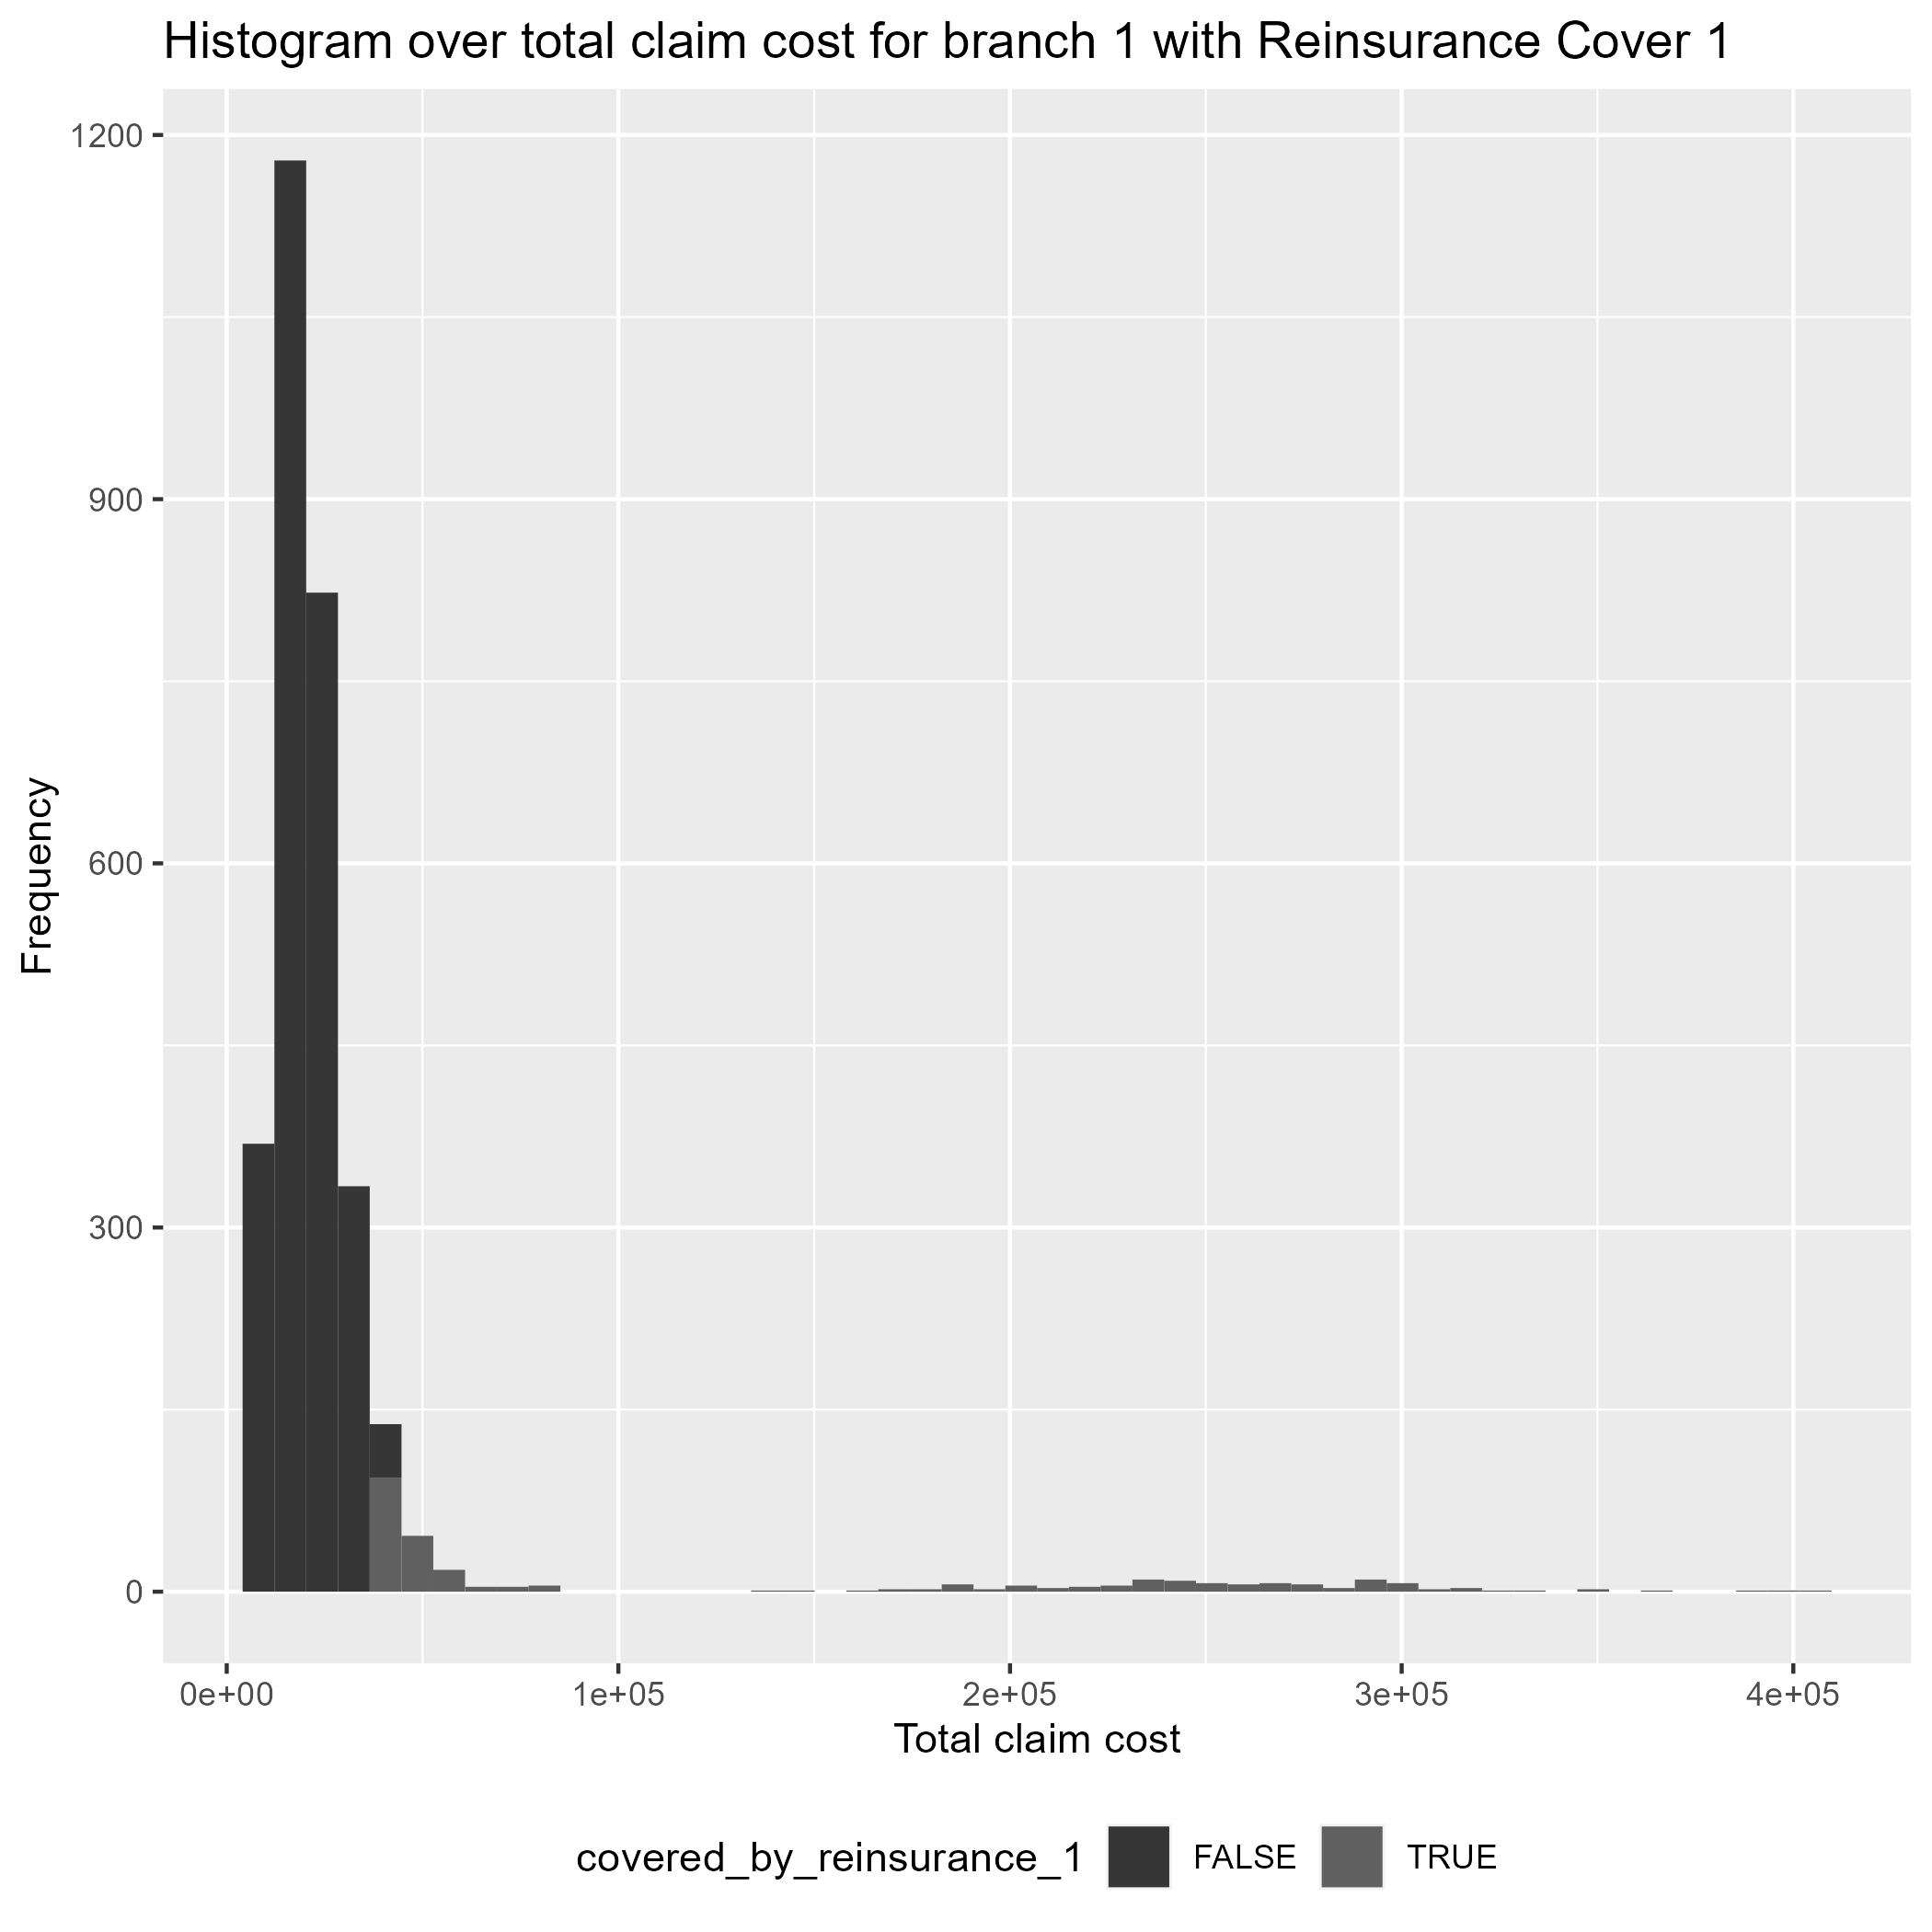
\includegraphics[width=.9\linewidth]{plots/reinsurance1/histogram_total_claim_cost_reinsurance1.png}
      \caption{Branch 1 Cost.}
    \end{subfigure}
    \begin{subfigure}{.24\textwidth}
      \centering
      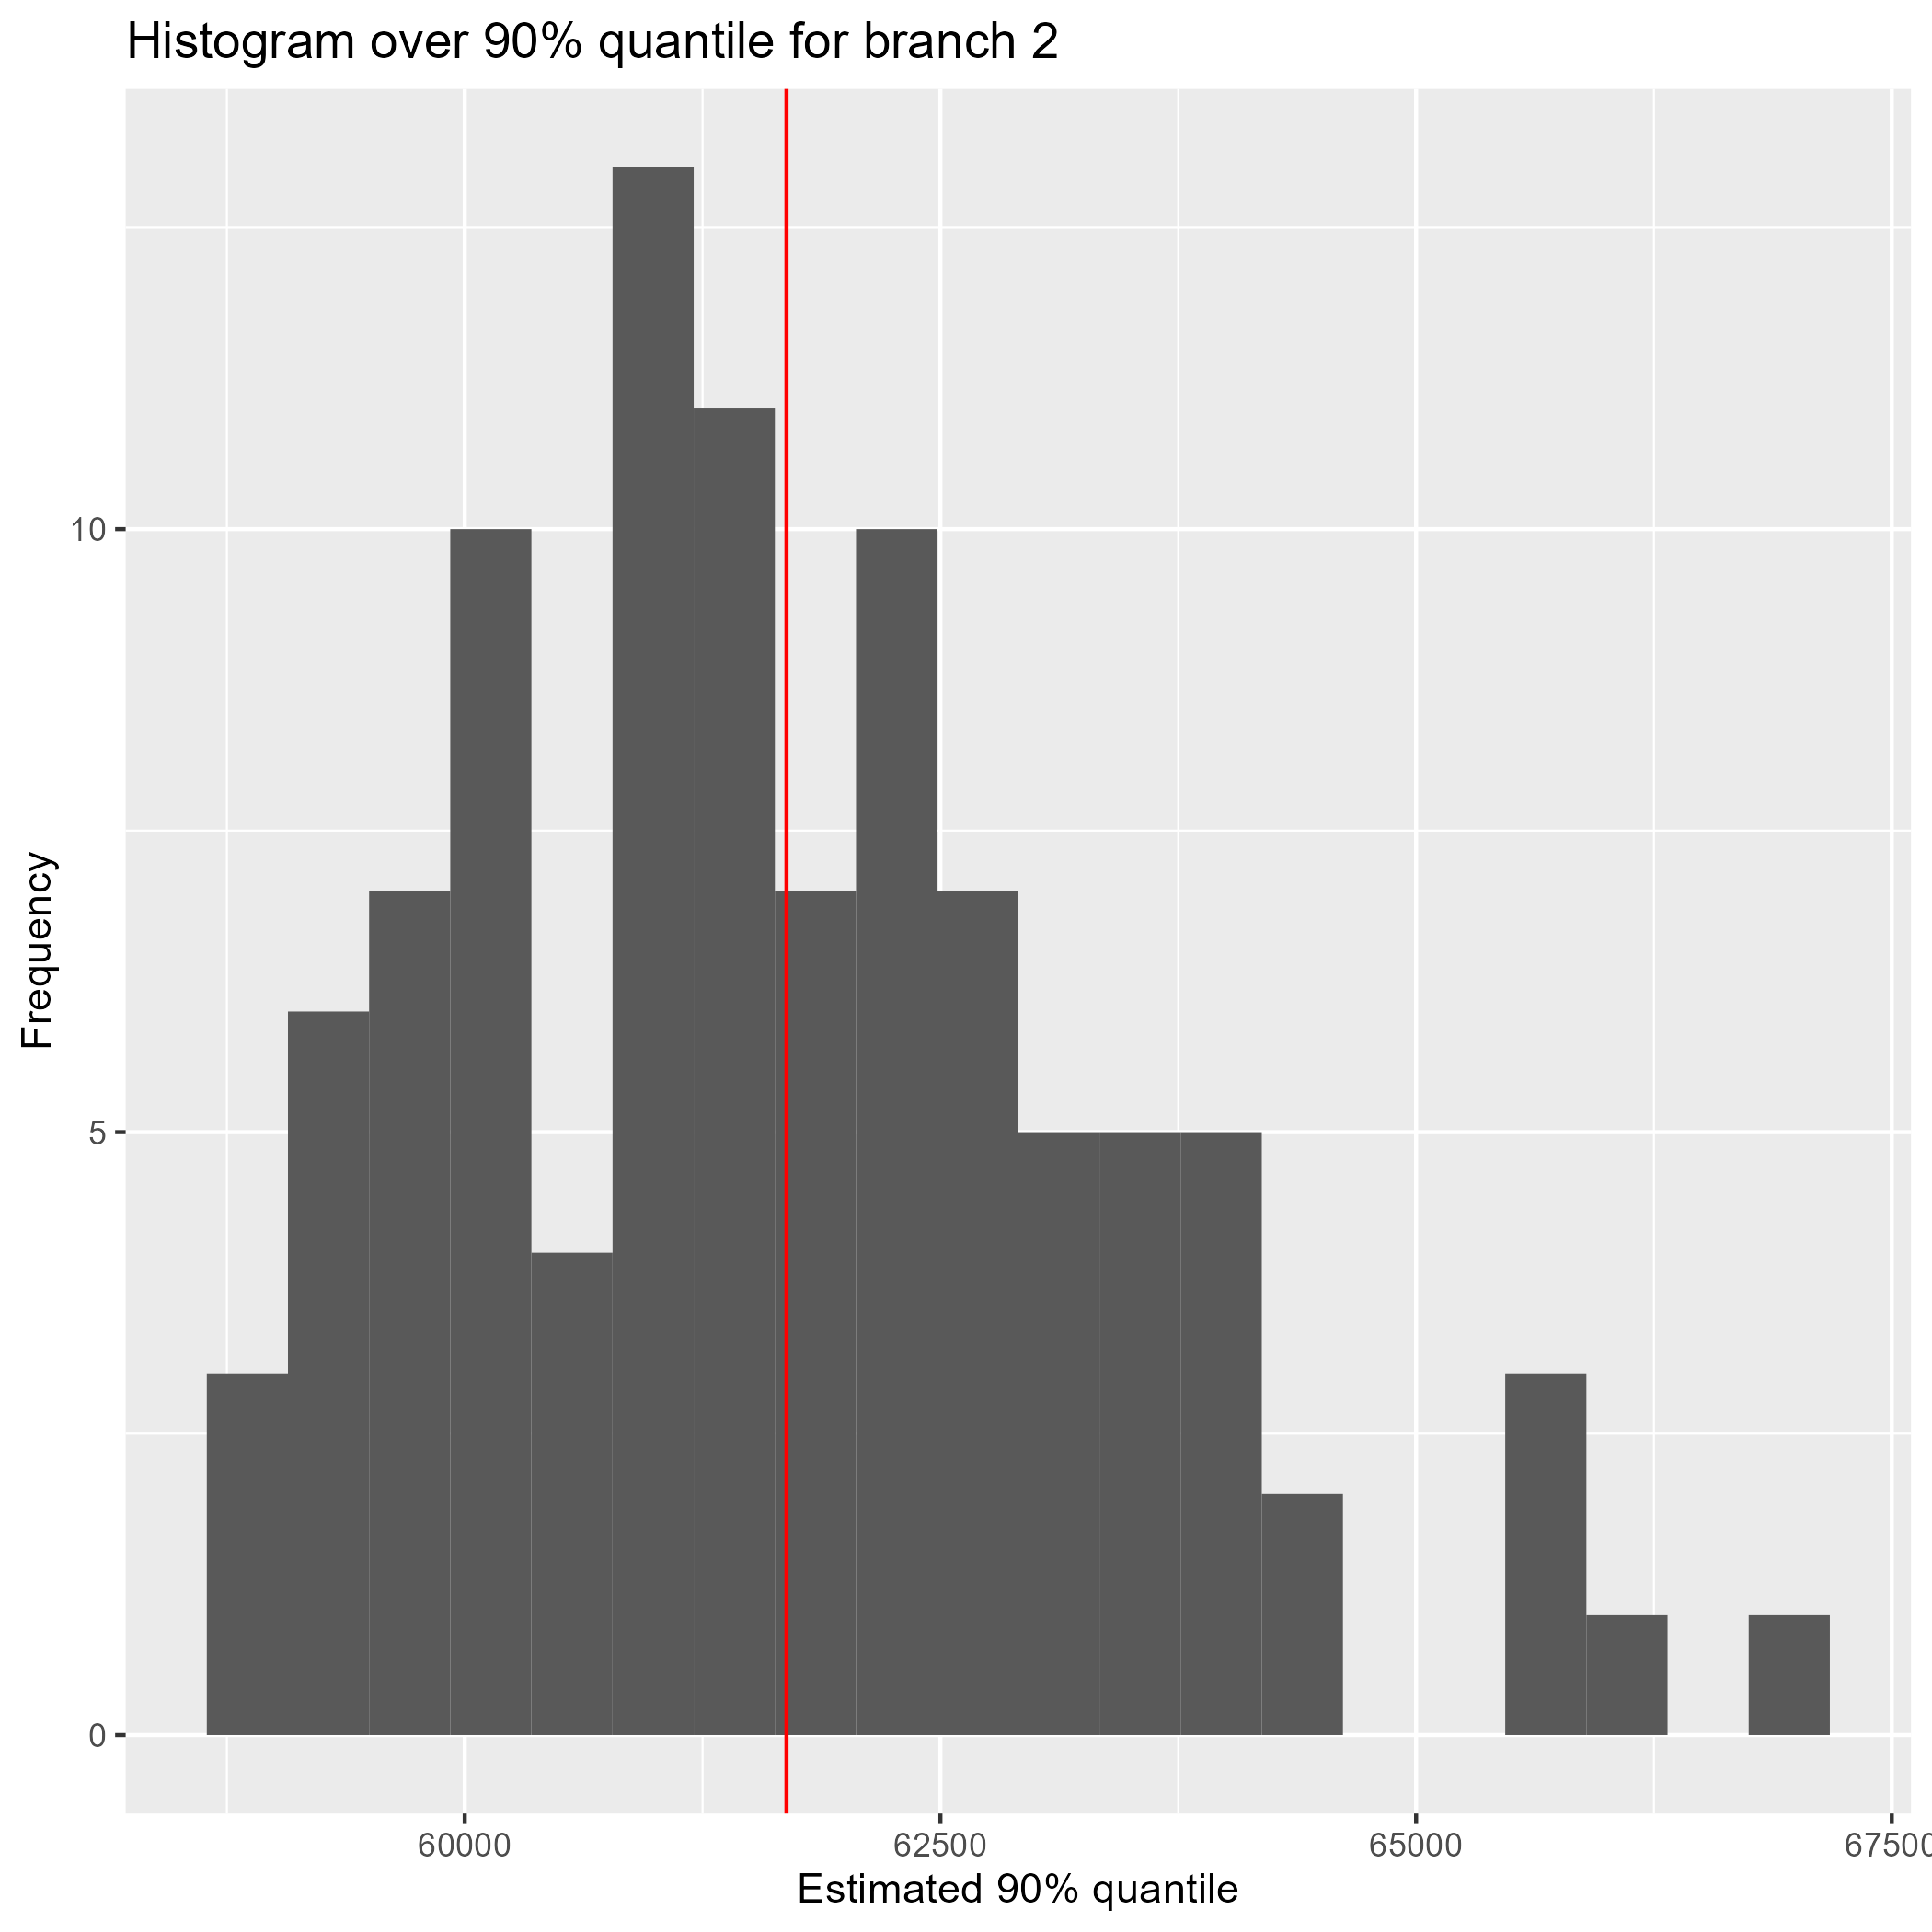
\includegraphics[width=.9\linewidth]{plots/reinsurance1/histogram_over_90p_quantile_2.png}
      \caption{Branch 2 Quantile.}
    \end{subfigure}
    \begin{subfigure}{.24\textwidth}
      \centering
      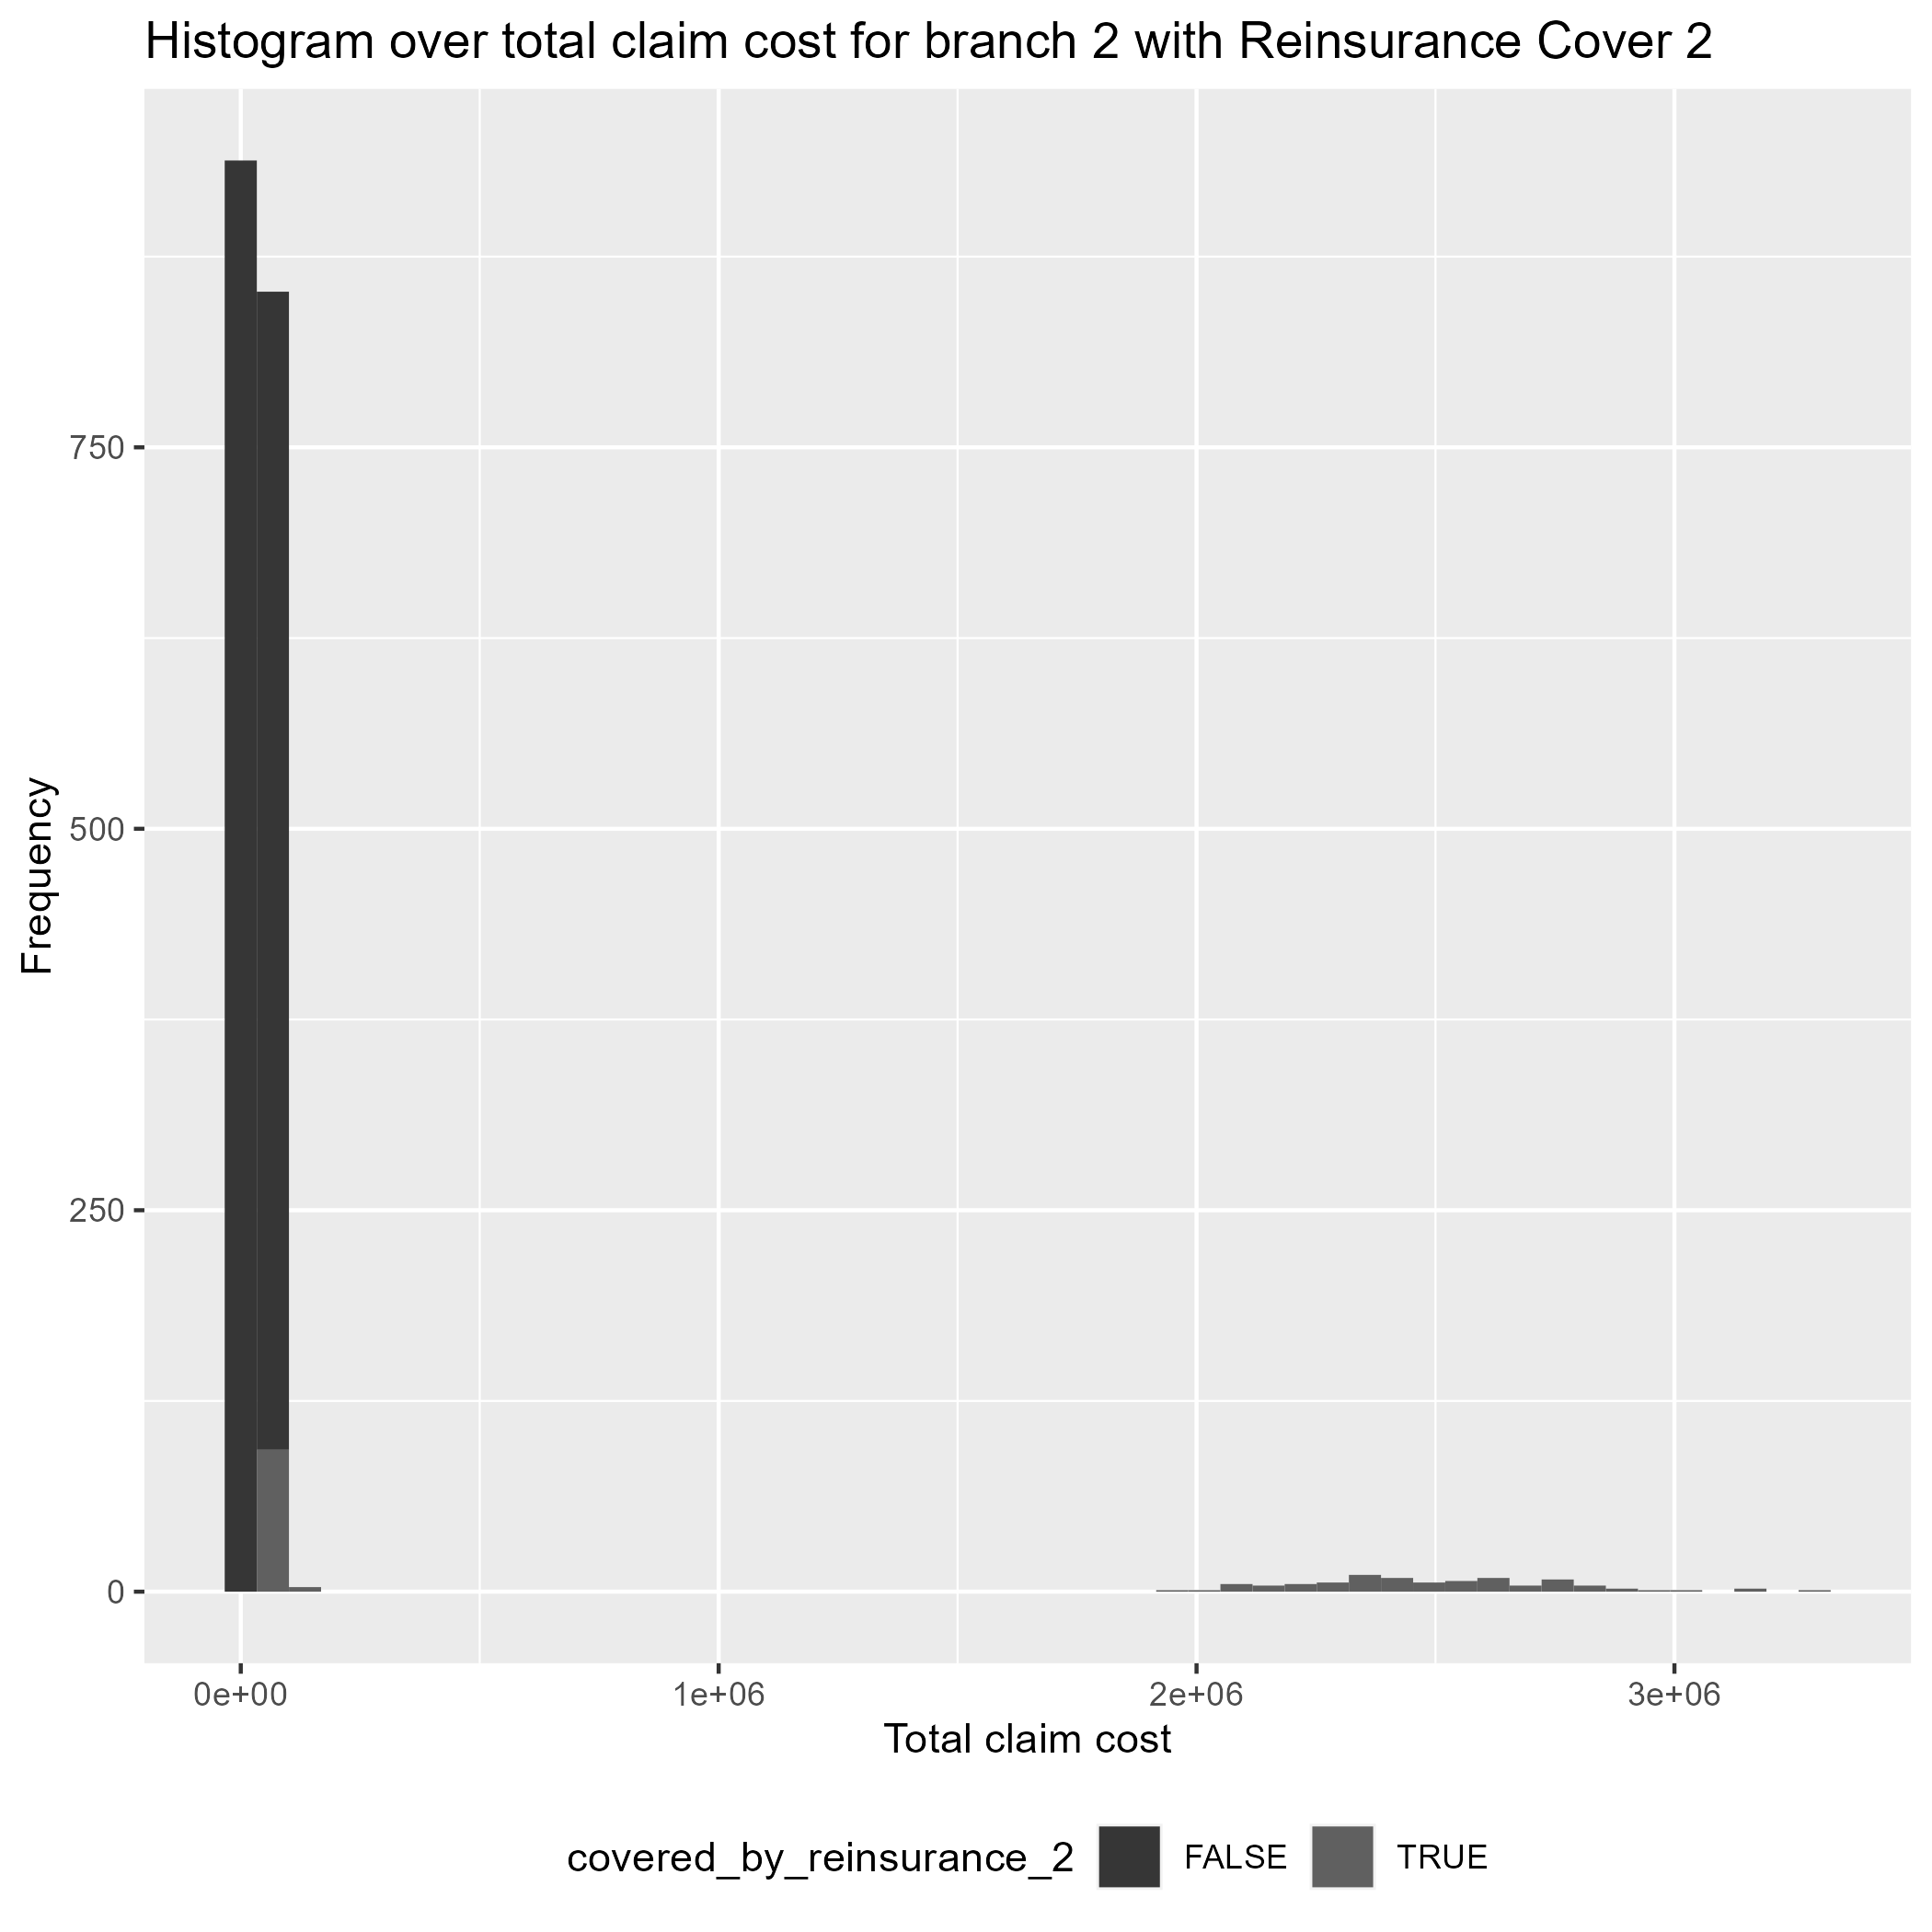
\includegraphics[width=.9\linewidth]{plots/reinsurance1/histogram_total_claim_cost_reinsurance2.png}
      \caption{Branch 2 Cost.}
    \end{subfigure}
    \caption{Estimated quantiles and impact on a simulated claim distribution.}
    \label{a5:simulation}
\end{figure}

Studying the final claim cost we see how reinsurance makes our results more stable, but less profitable.
Seen in figure  \ref{a5:claim_cost} we observe how the total claim cost is more varied with reinsurance compared to without.
On the contrary, we see that the savings are rarely positive, likely because of the $120\%$ of expected cost price of reinsurance means that we need circumstances which imply many large claims above the expected.
In the scenario of extreme events, like extreme weather or natural perils, this reinsurance could be reasonable, but we need a good indication to value this stability towards the price we pay.

 \begin{figure}[!h]
\centering
    \begin{subfigure}{.49\textwidth}
      \centering
      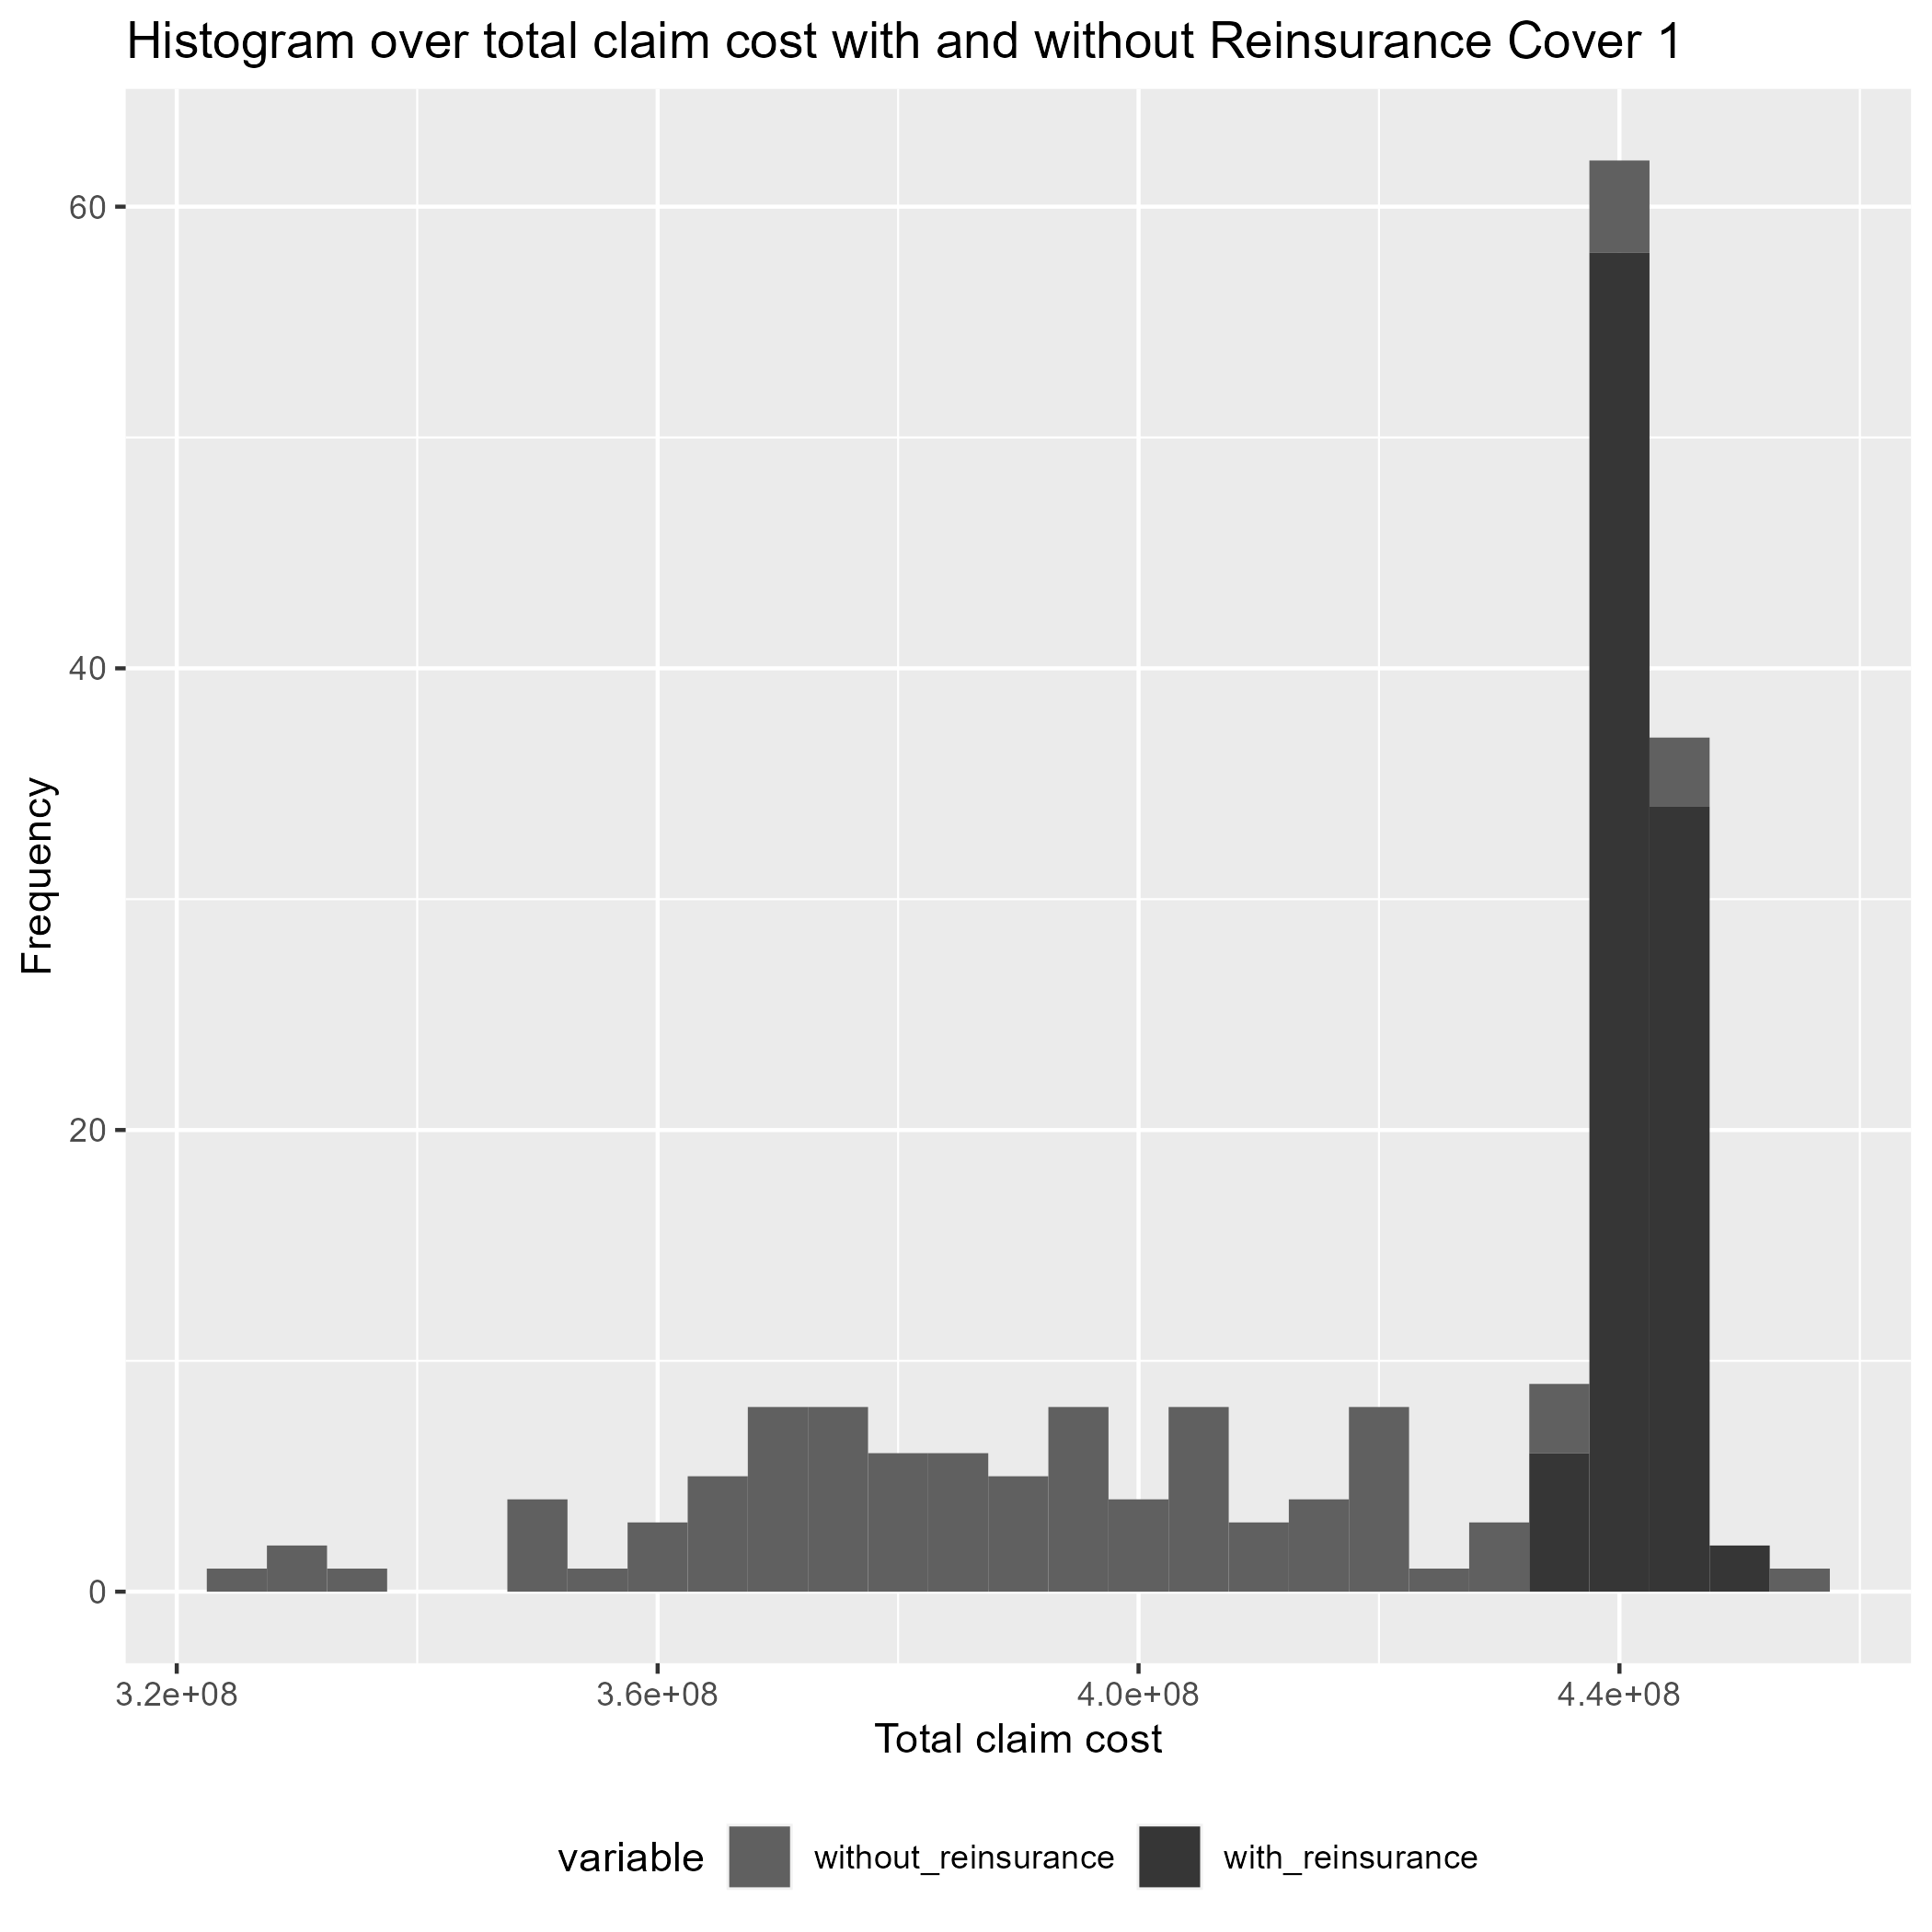
\includegraphics[width=.9\linewidth]{plots/reinsurance1/histogram_total_claim_cost_with_reinsurance.png}
      \caption{Distribution of total claim amounts.}
    \end{subfigure}
    \begin{subfigure}{.49\textwidth}
      \centering
      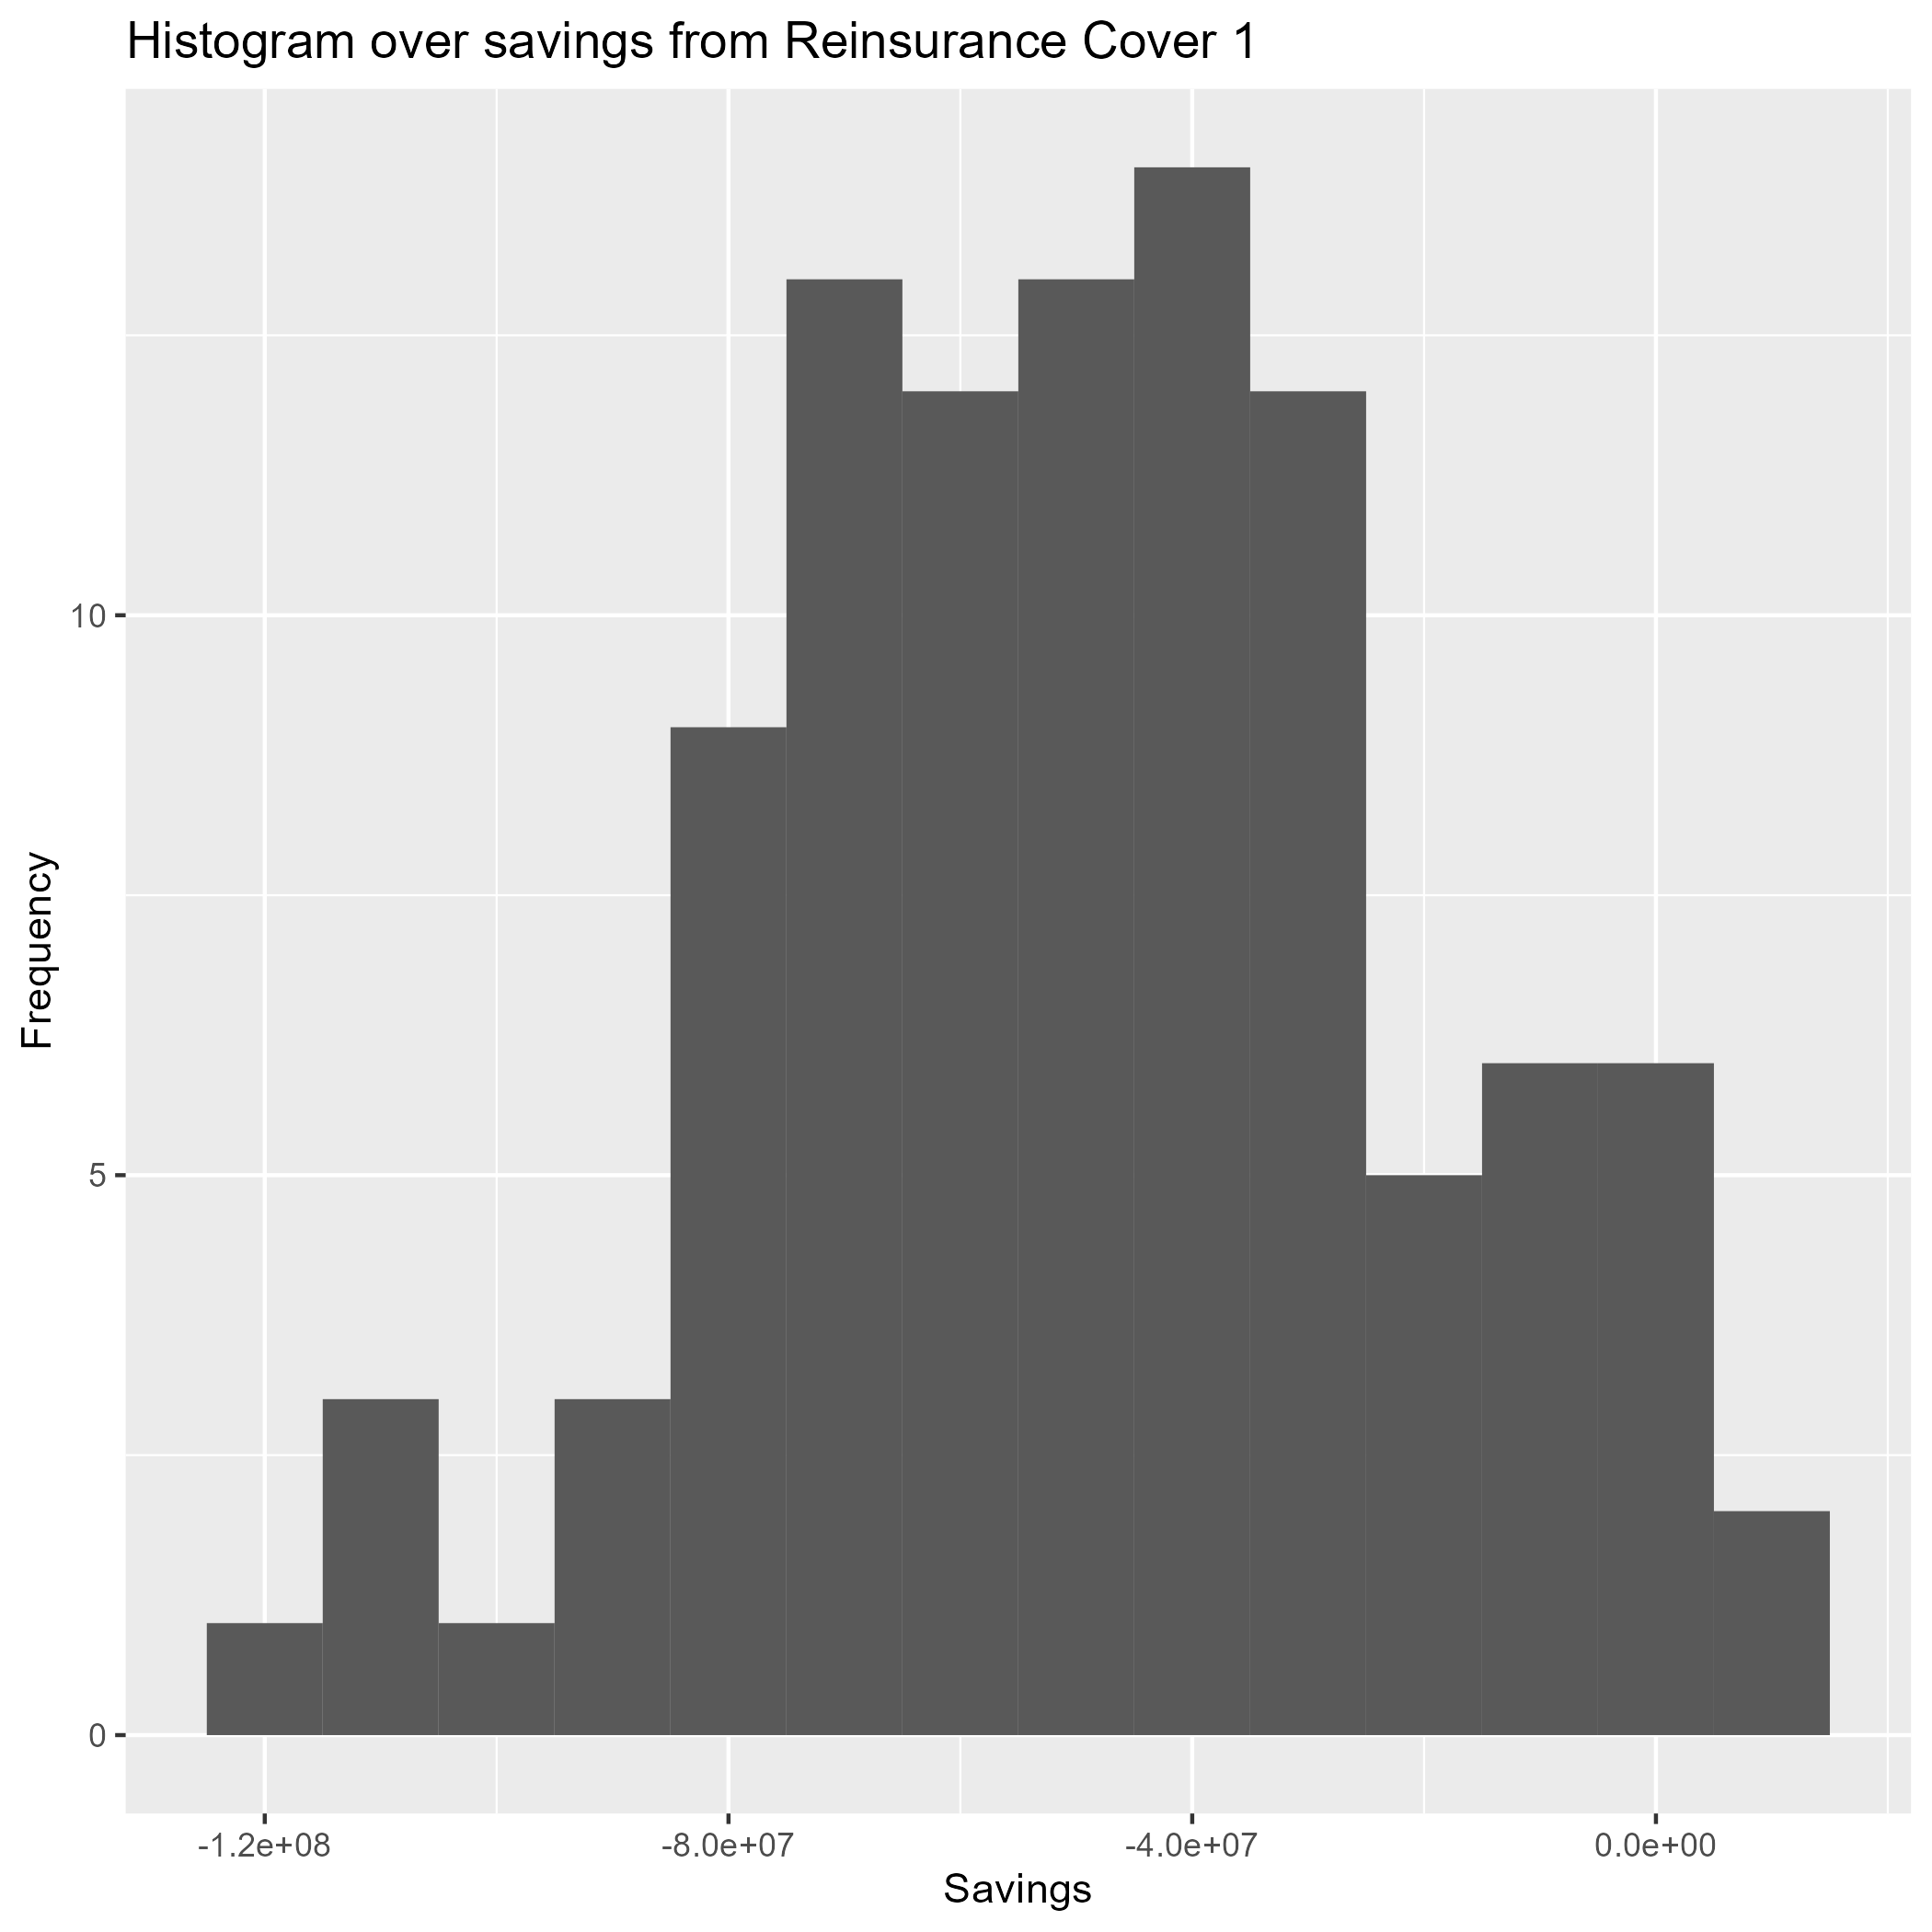
\includegraphics[width=.9\linewidth]{plots/reinsurance1/histogram_savings.png}
      \caption{Savings with Reinsurance.}
    \end{subfigure}
    \caption{Estimated quantiles and impact on a simulated claim distribution.}
    \label{a5:claim_cost}
\end{figure}


\subsubsection*{The SL Cover}

In applying the SL cover we study how the final total claim cost per branch can be limited through percentile analysis.
Estimating these quantiles and plotting the final claim cost with and without reinsurance cover, we get the results shown in figure \ref{a6:simulation}.
As can be seen the percentiles is more apperant here compared to the XL-cover, where the claim-cost was on individual cases.

 \begin{figure}[!h]
\centering
    \begin{subfigure}{.24\textwidth}
      \centering
      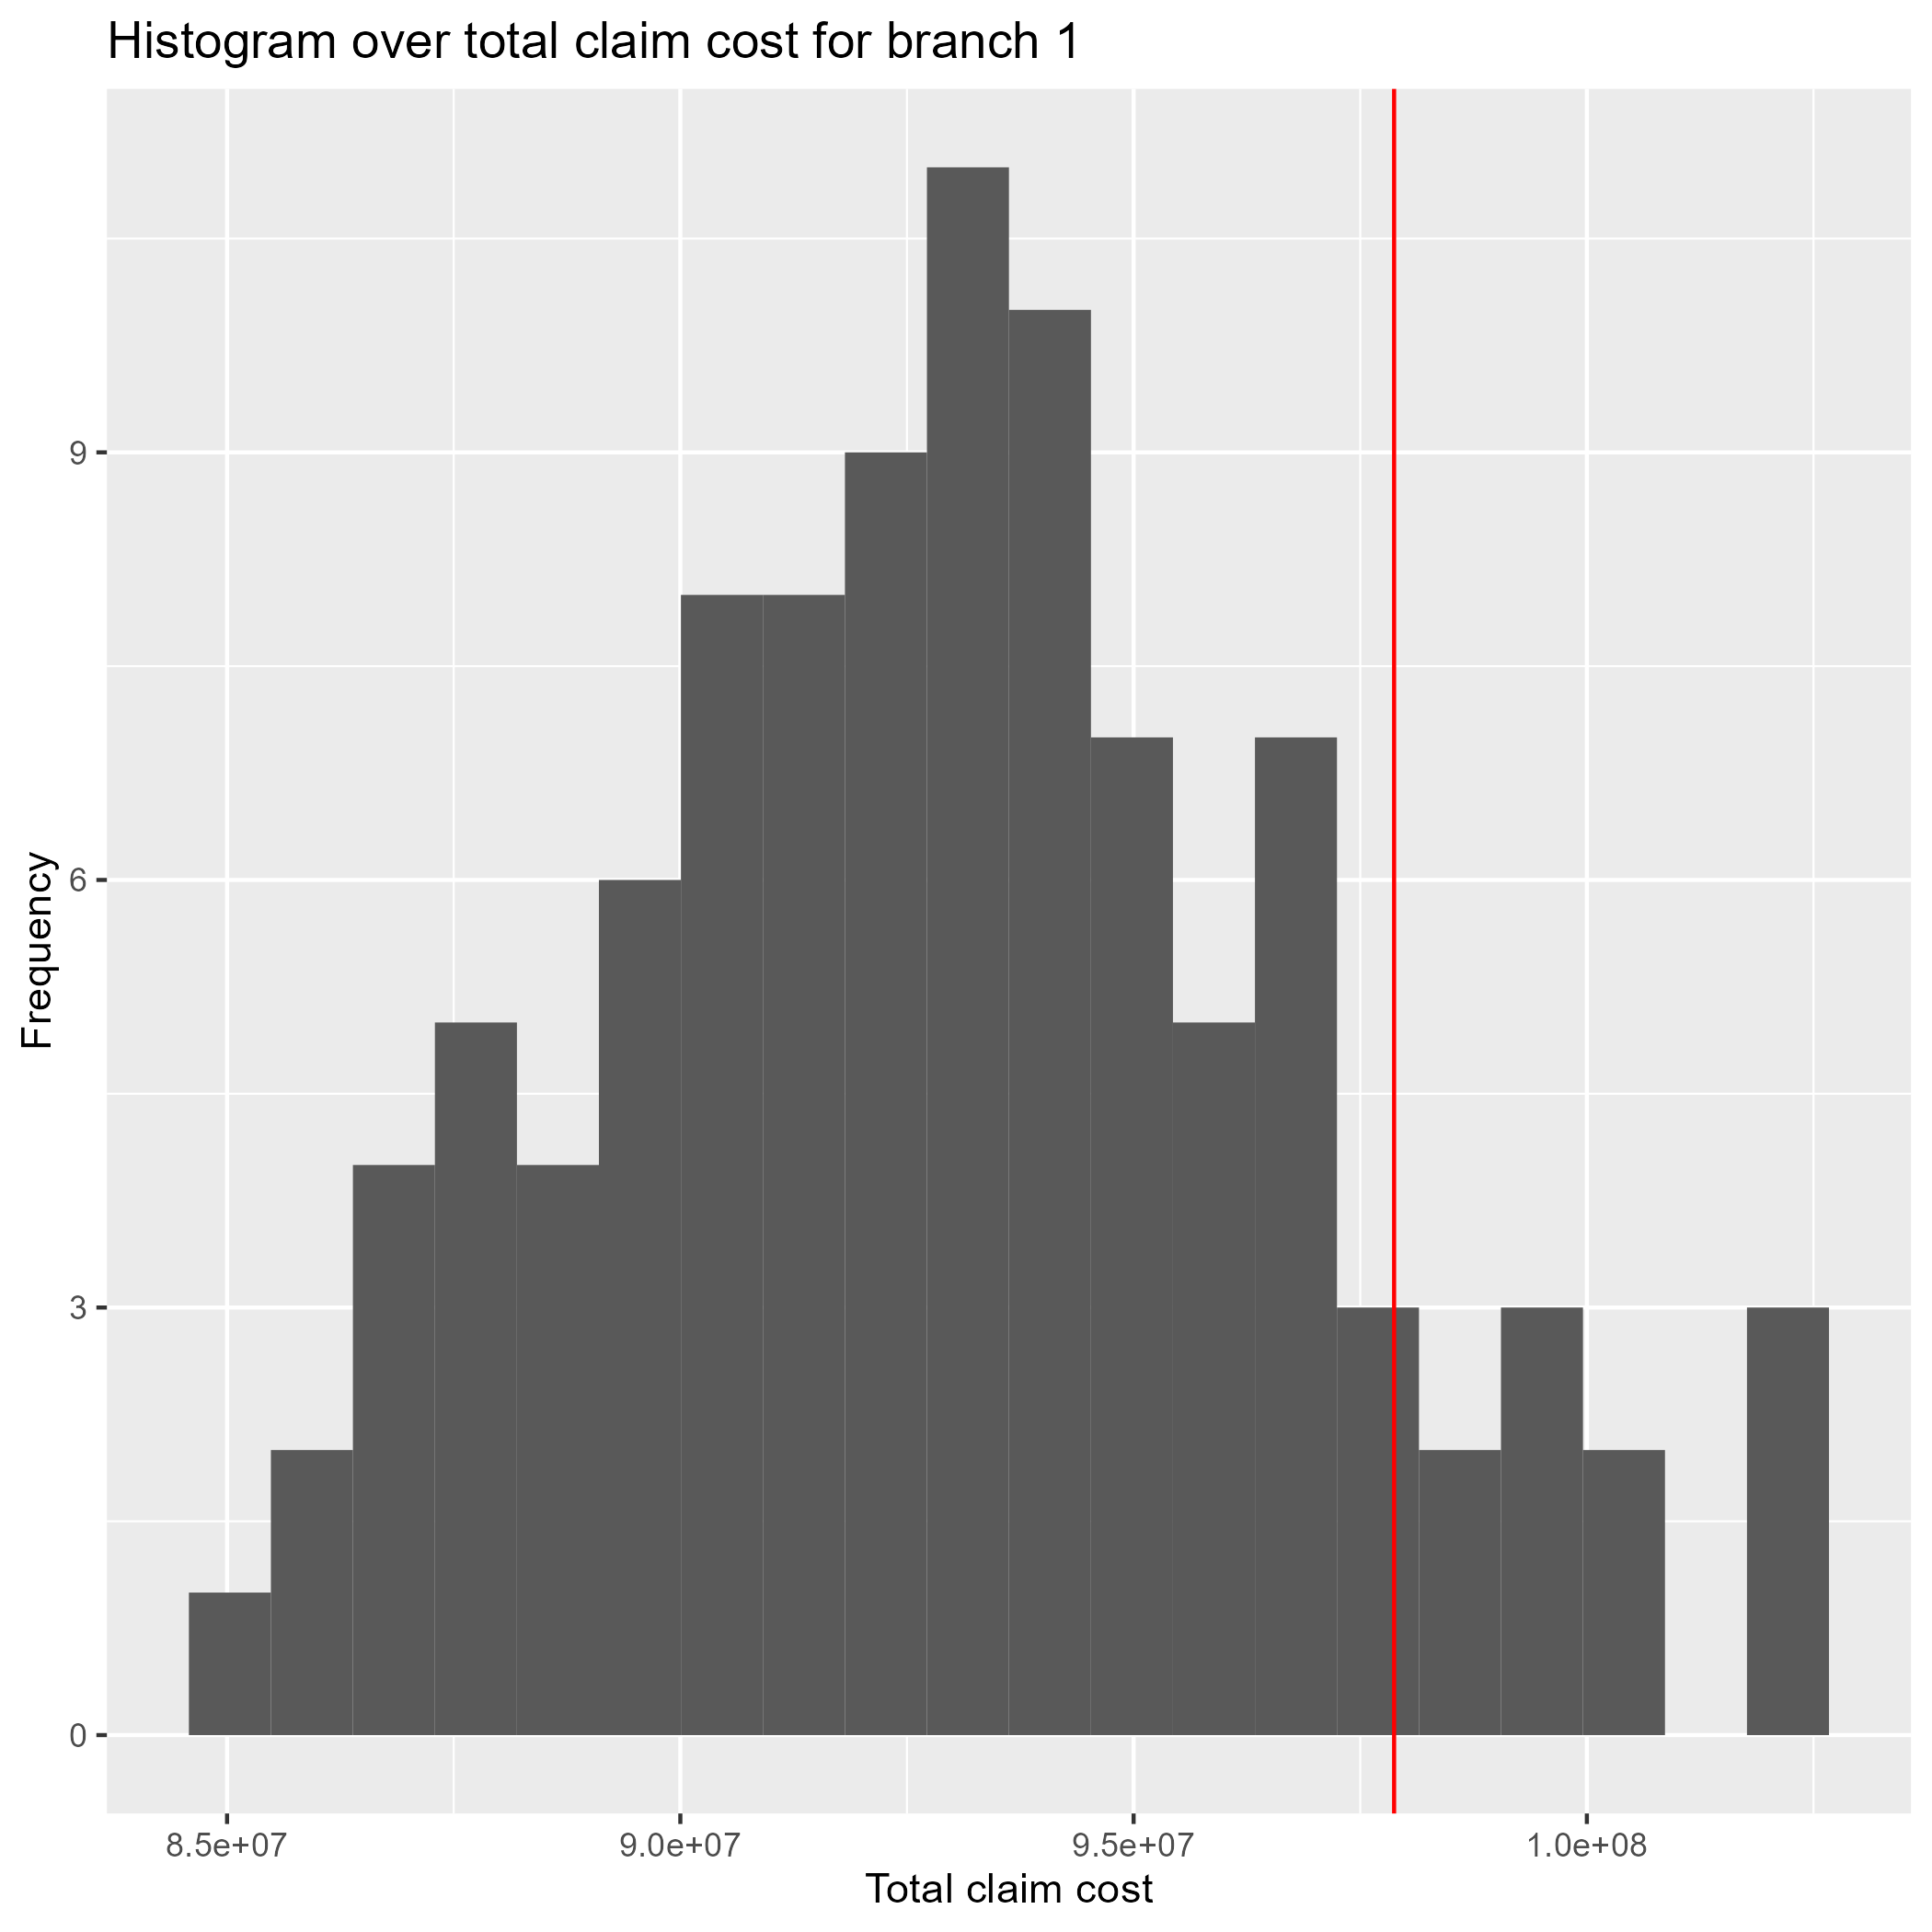
\includegraphics[width=.9\linewidth]{plots/reinsurance2/histogram_over_90p_quantile_1.png}
      \caption{Branch 1 Quantile.}
    \end{subfigure}
    \begin{subfigure}{.24\textwidth}
      \centering
      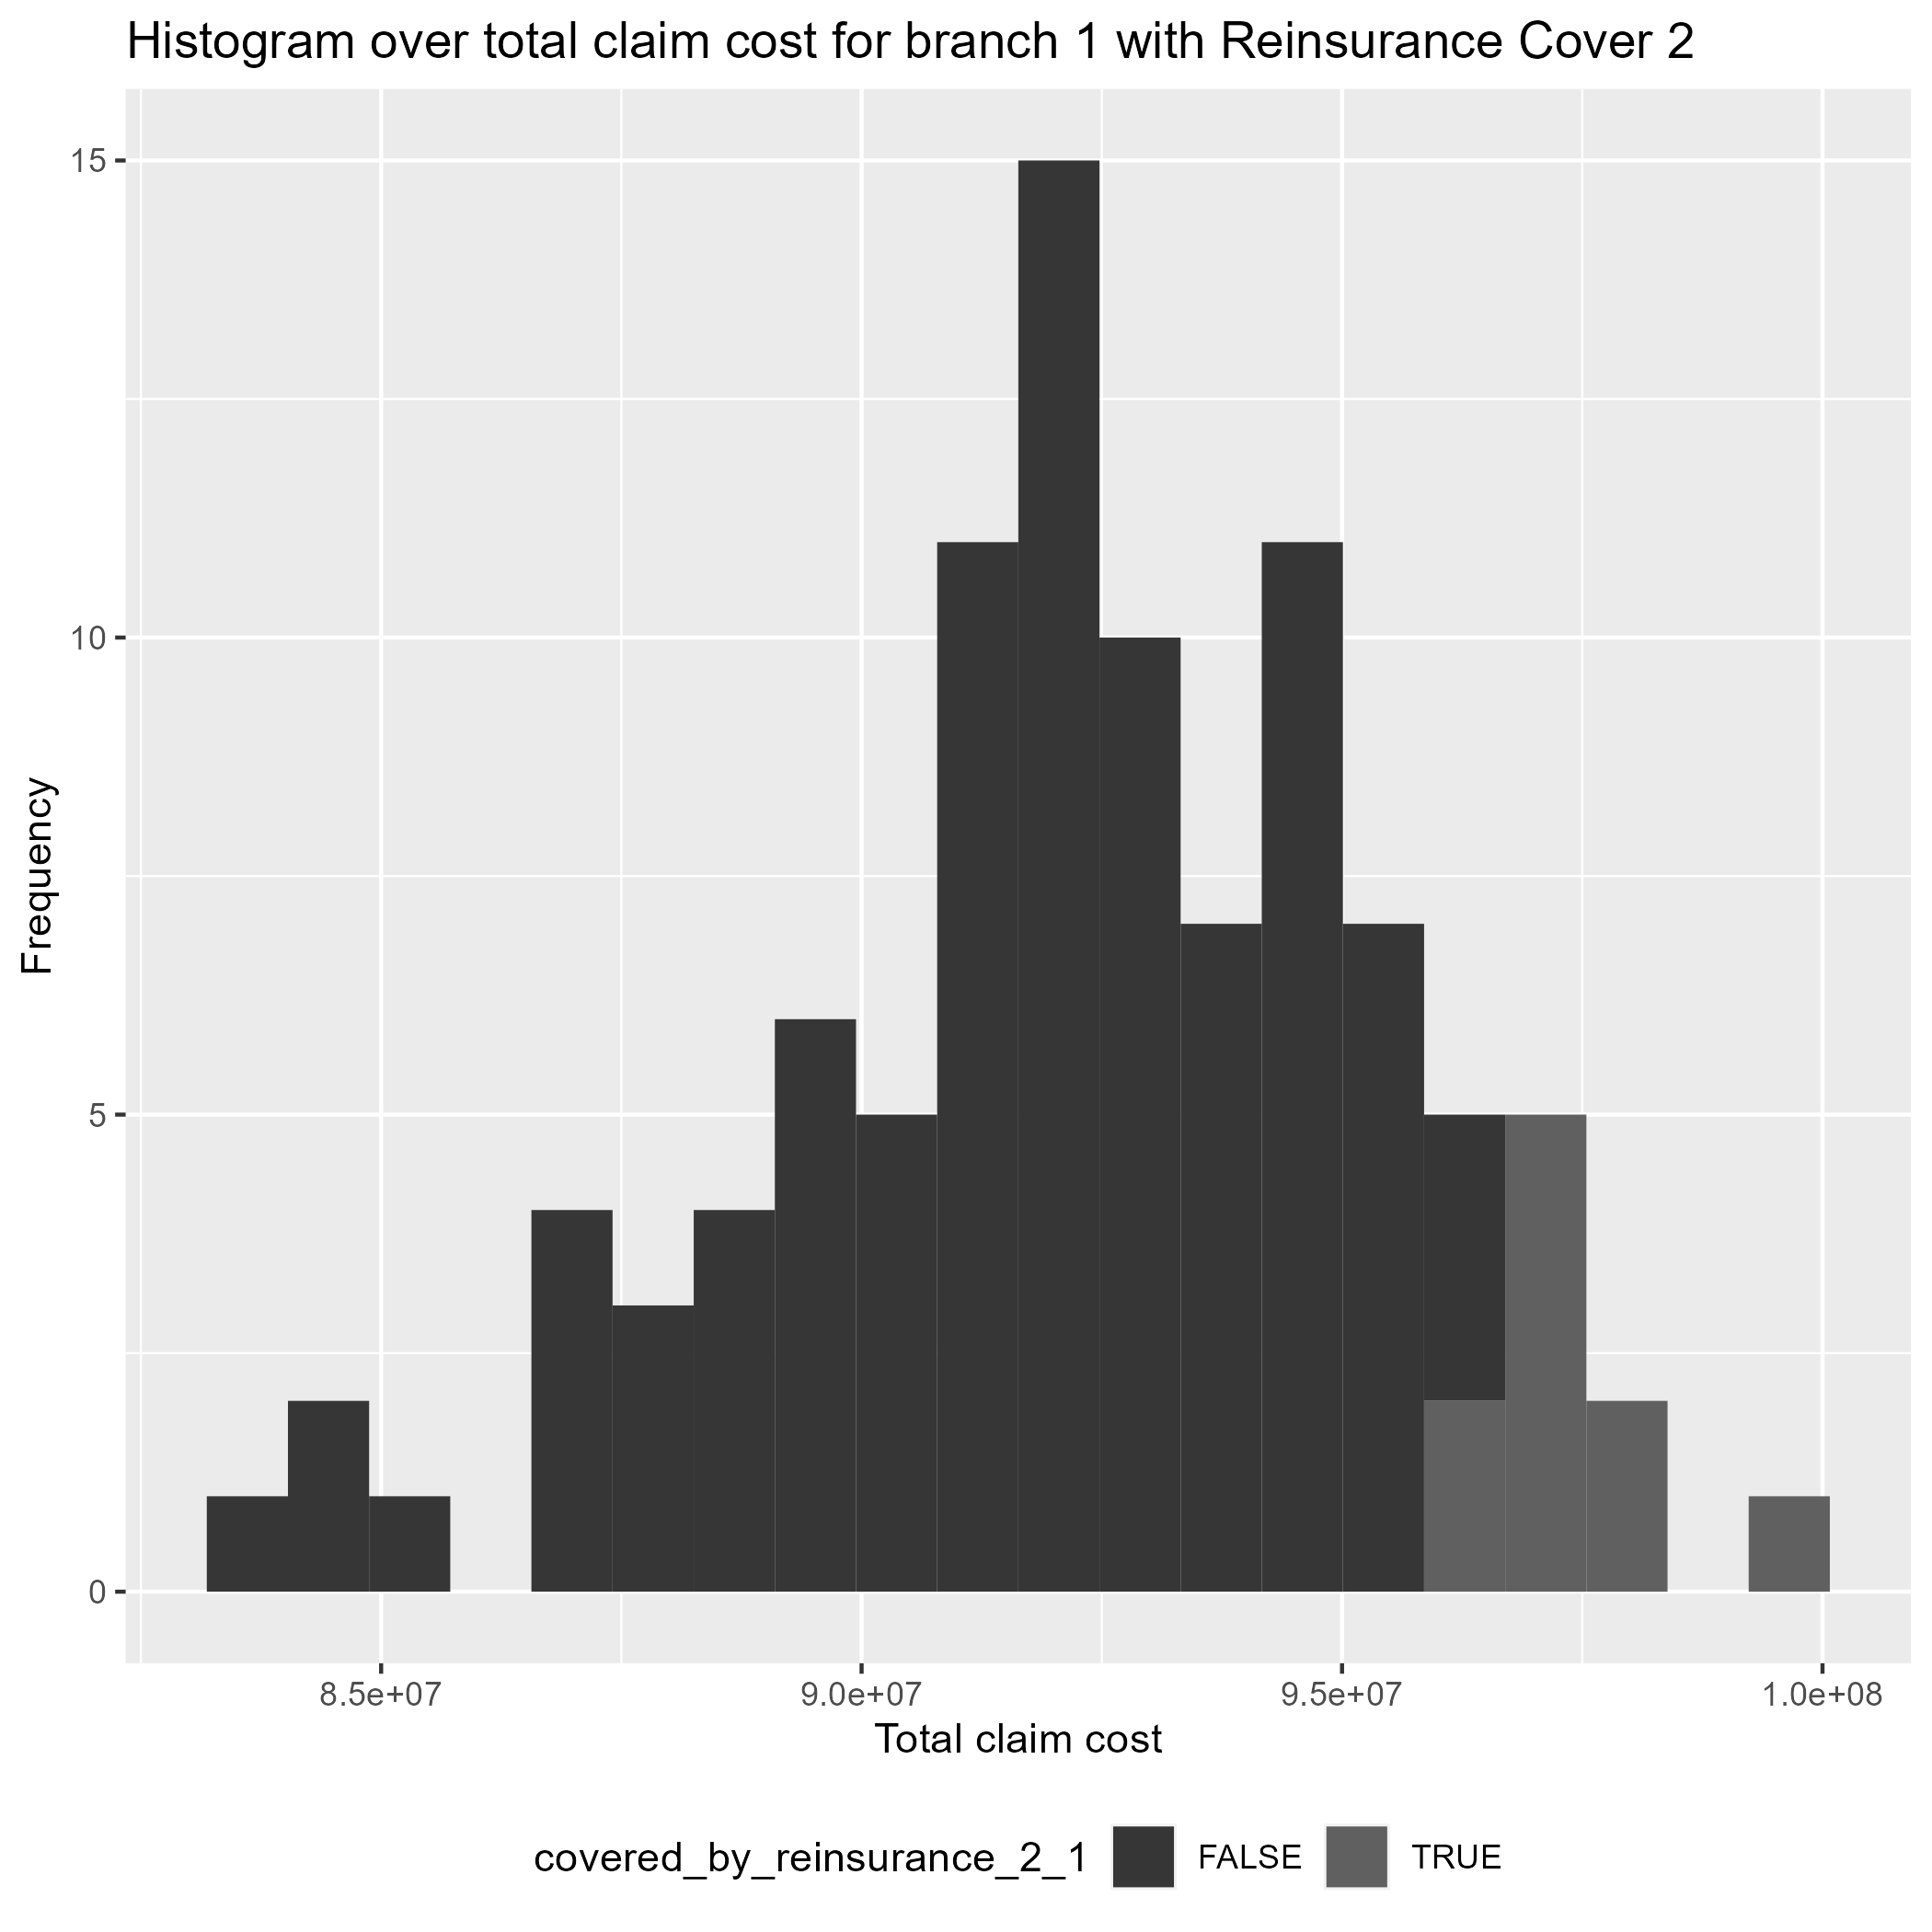
\includegraphics[width=.9\linewidth]{plots/reinsurance2/histogram_total_claim_cost_reinsurance2_1.png}
      \caption{Branch 1 Cost.}
    \end{subfigure}
    \begin{subfigure}{.24\textwidth}
      \centering
      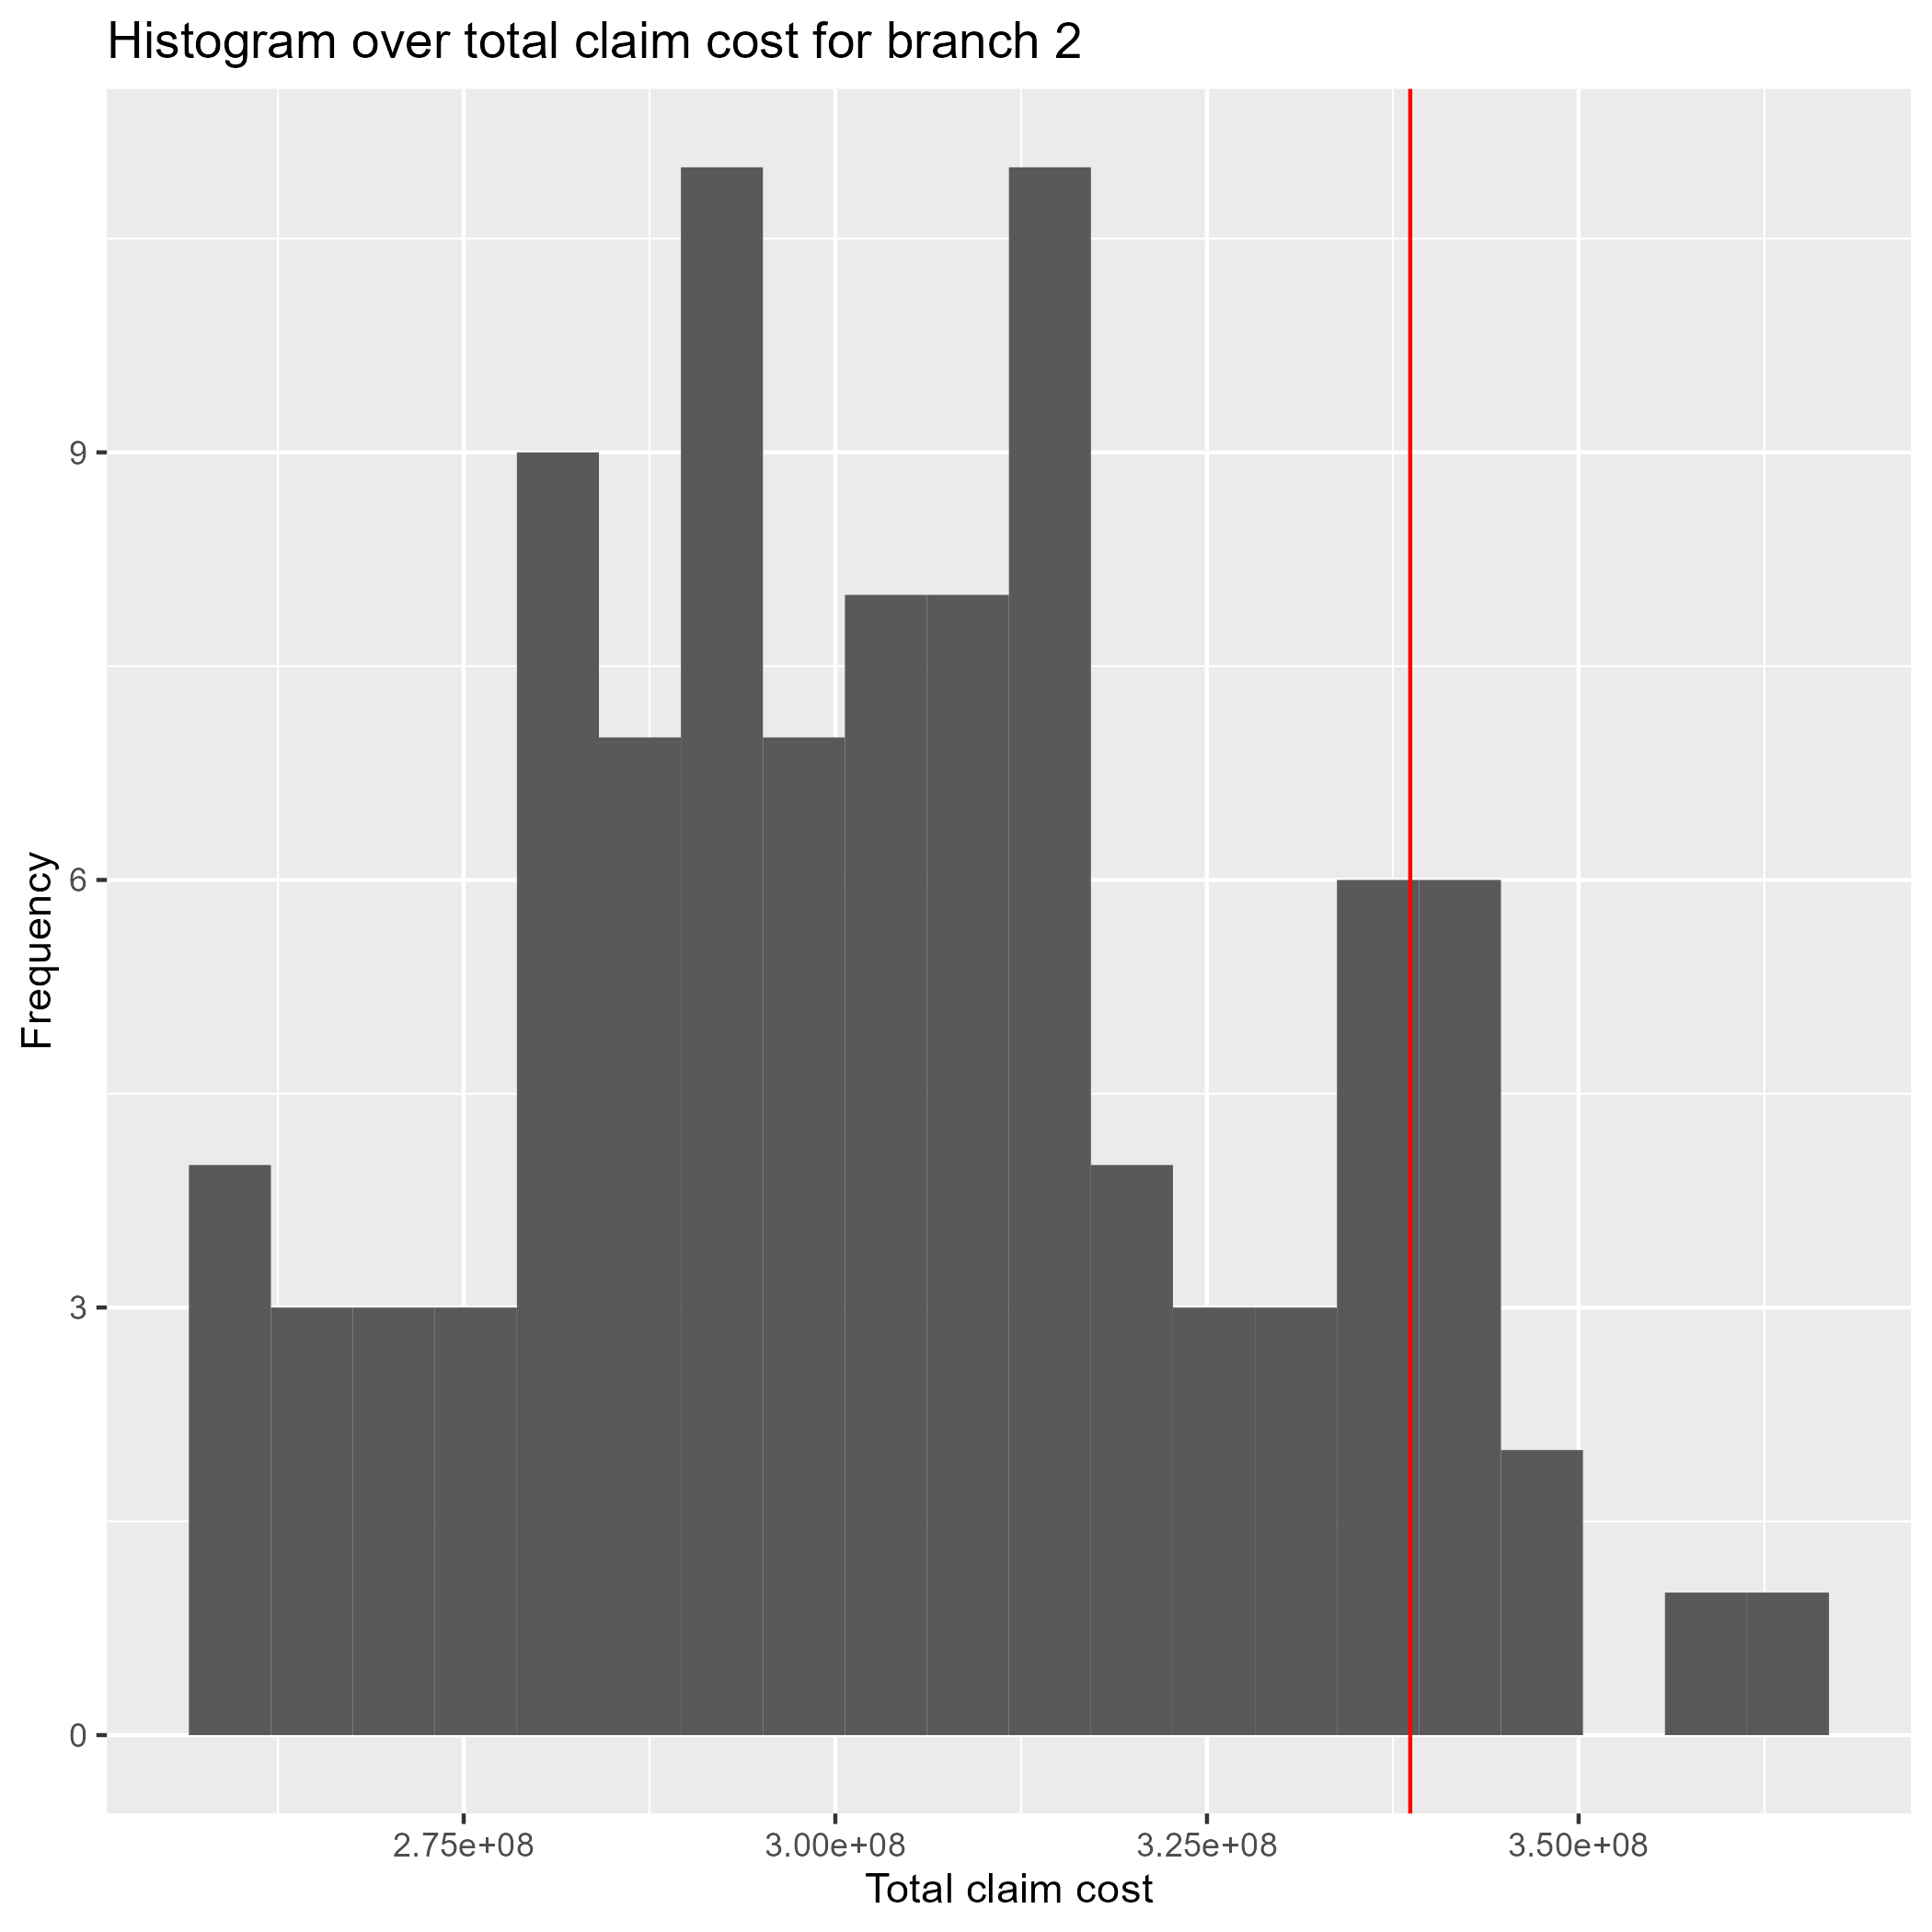
\includegraphics[width=.9\linewidth]{plots/reinsurance2/histogram_over_90p_quantile_2.png}
      \caption{Branch 2 Quantile.}
    \end{subfigure}
    \begin{subfigure}{.24\textwidth}
      \centering
      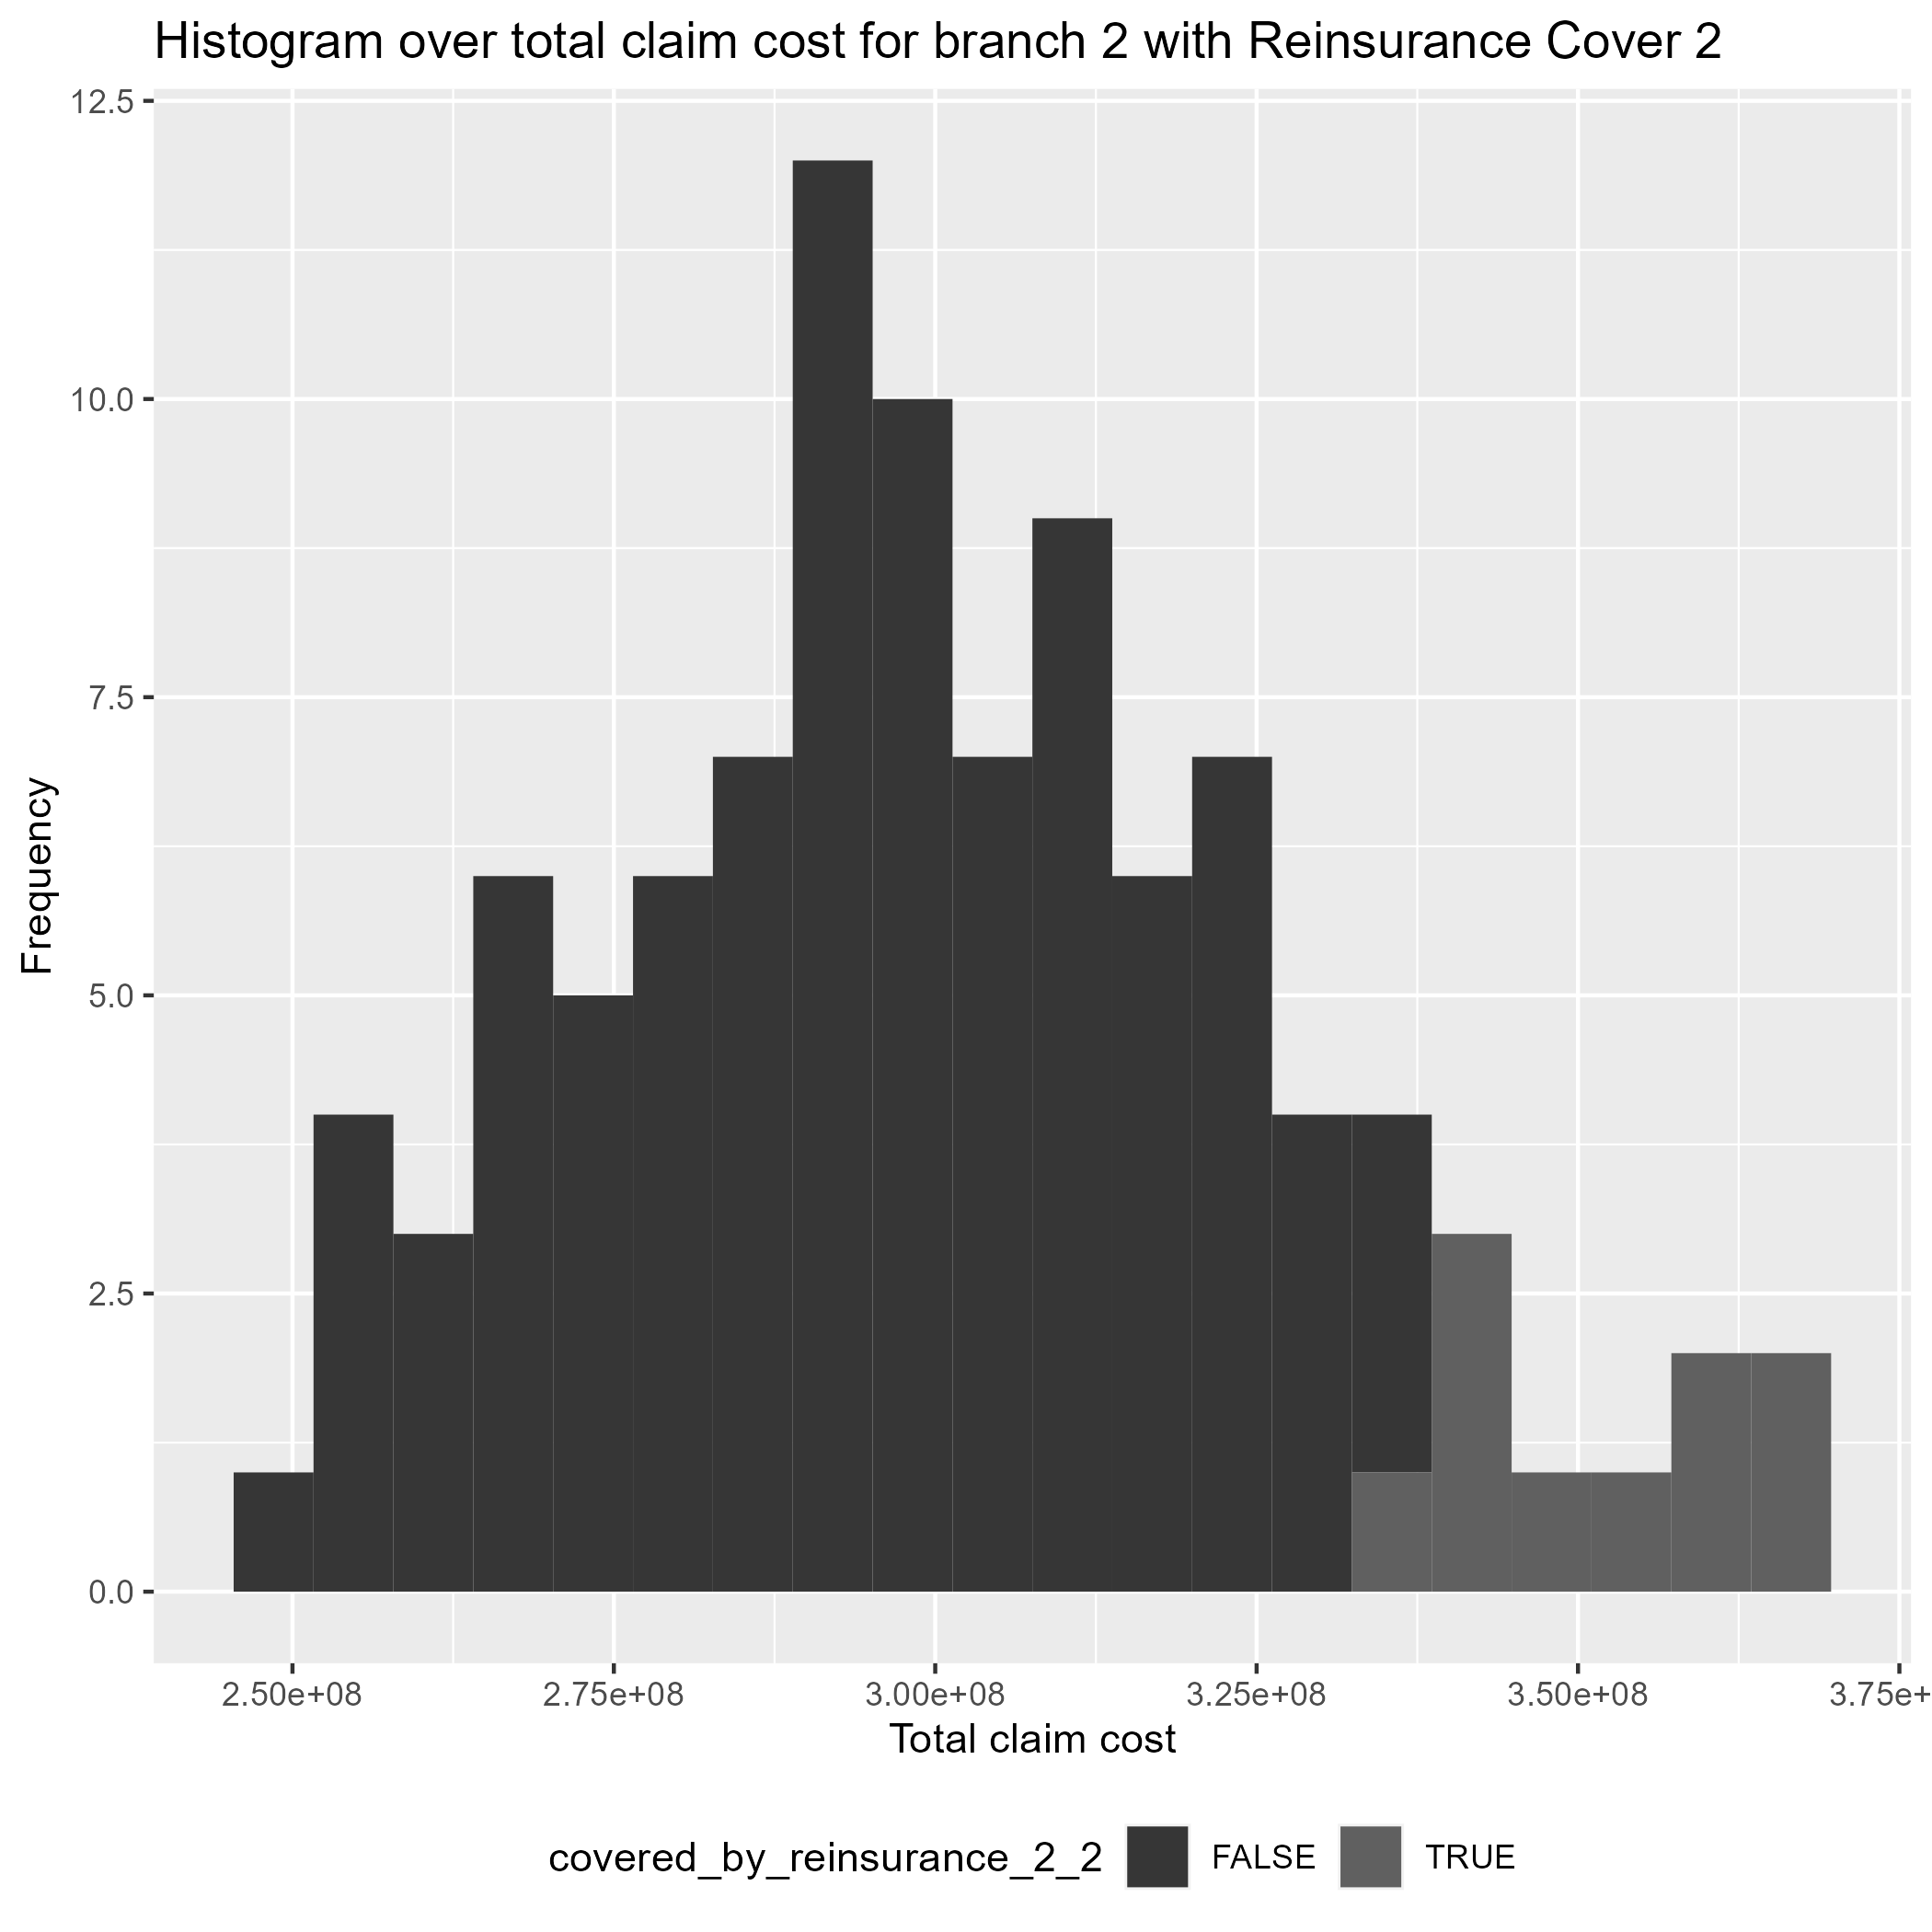
\includegraphics[width=.9\linewidth]{plots/reinsurance2/histogram_total_claim_cost_reinsurance2_2.png}
      \caption{Branch 2 Cost.}
    \end{subfigure}
    \caption{Estimated quantiles and impact on a simulated claim distribution.}
    \label{a6:simulation}
\end{figure}

Studying the final claim cost we observe that we rarely get use of the reinsurance.
This is seen in figre \ref{a6:claim_cost}, where the savings tend to be mostly negative, and only barely do we get a scenario that our total claims exceeds the 20\% excess point of the cutoff.
Even in cases with us exceeding the cut-off we rarely get value out of the reinsurance.
An alternative would be if we want to only reinsurance one of the branches, and not the other, but this is out of the scope of this question.

 \begin{figure}[!h]
\centering
    \begin{subfigure}{.49\textwidth}
      \centering
      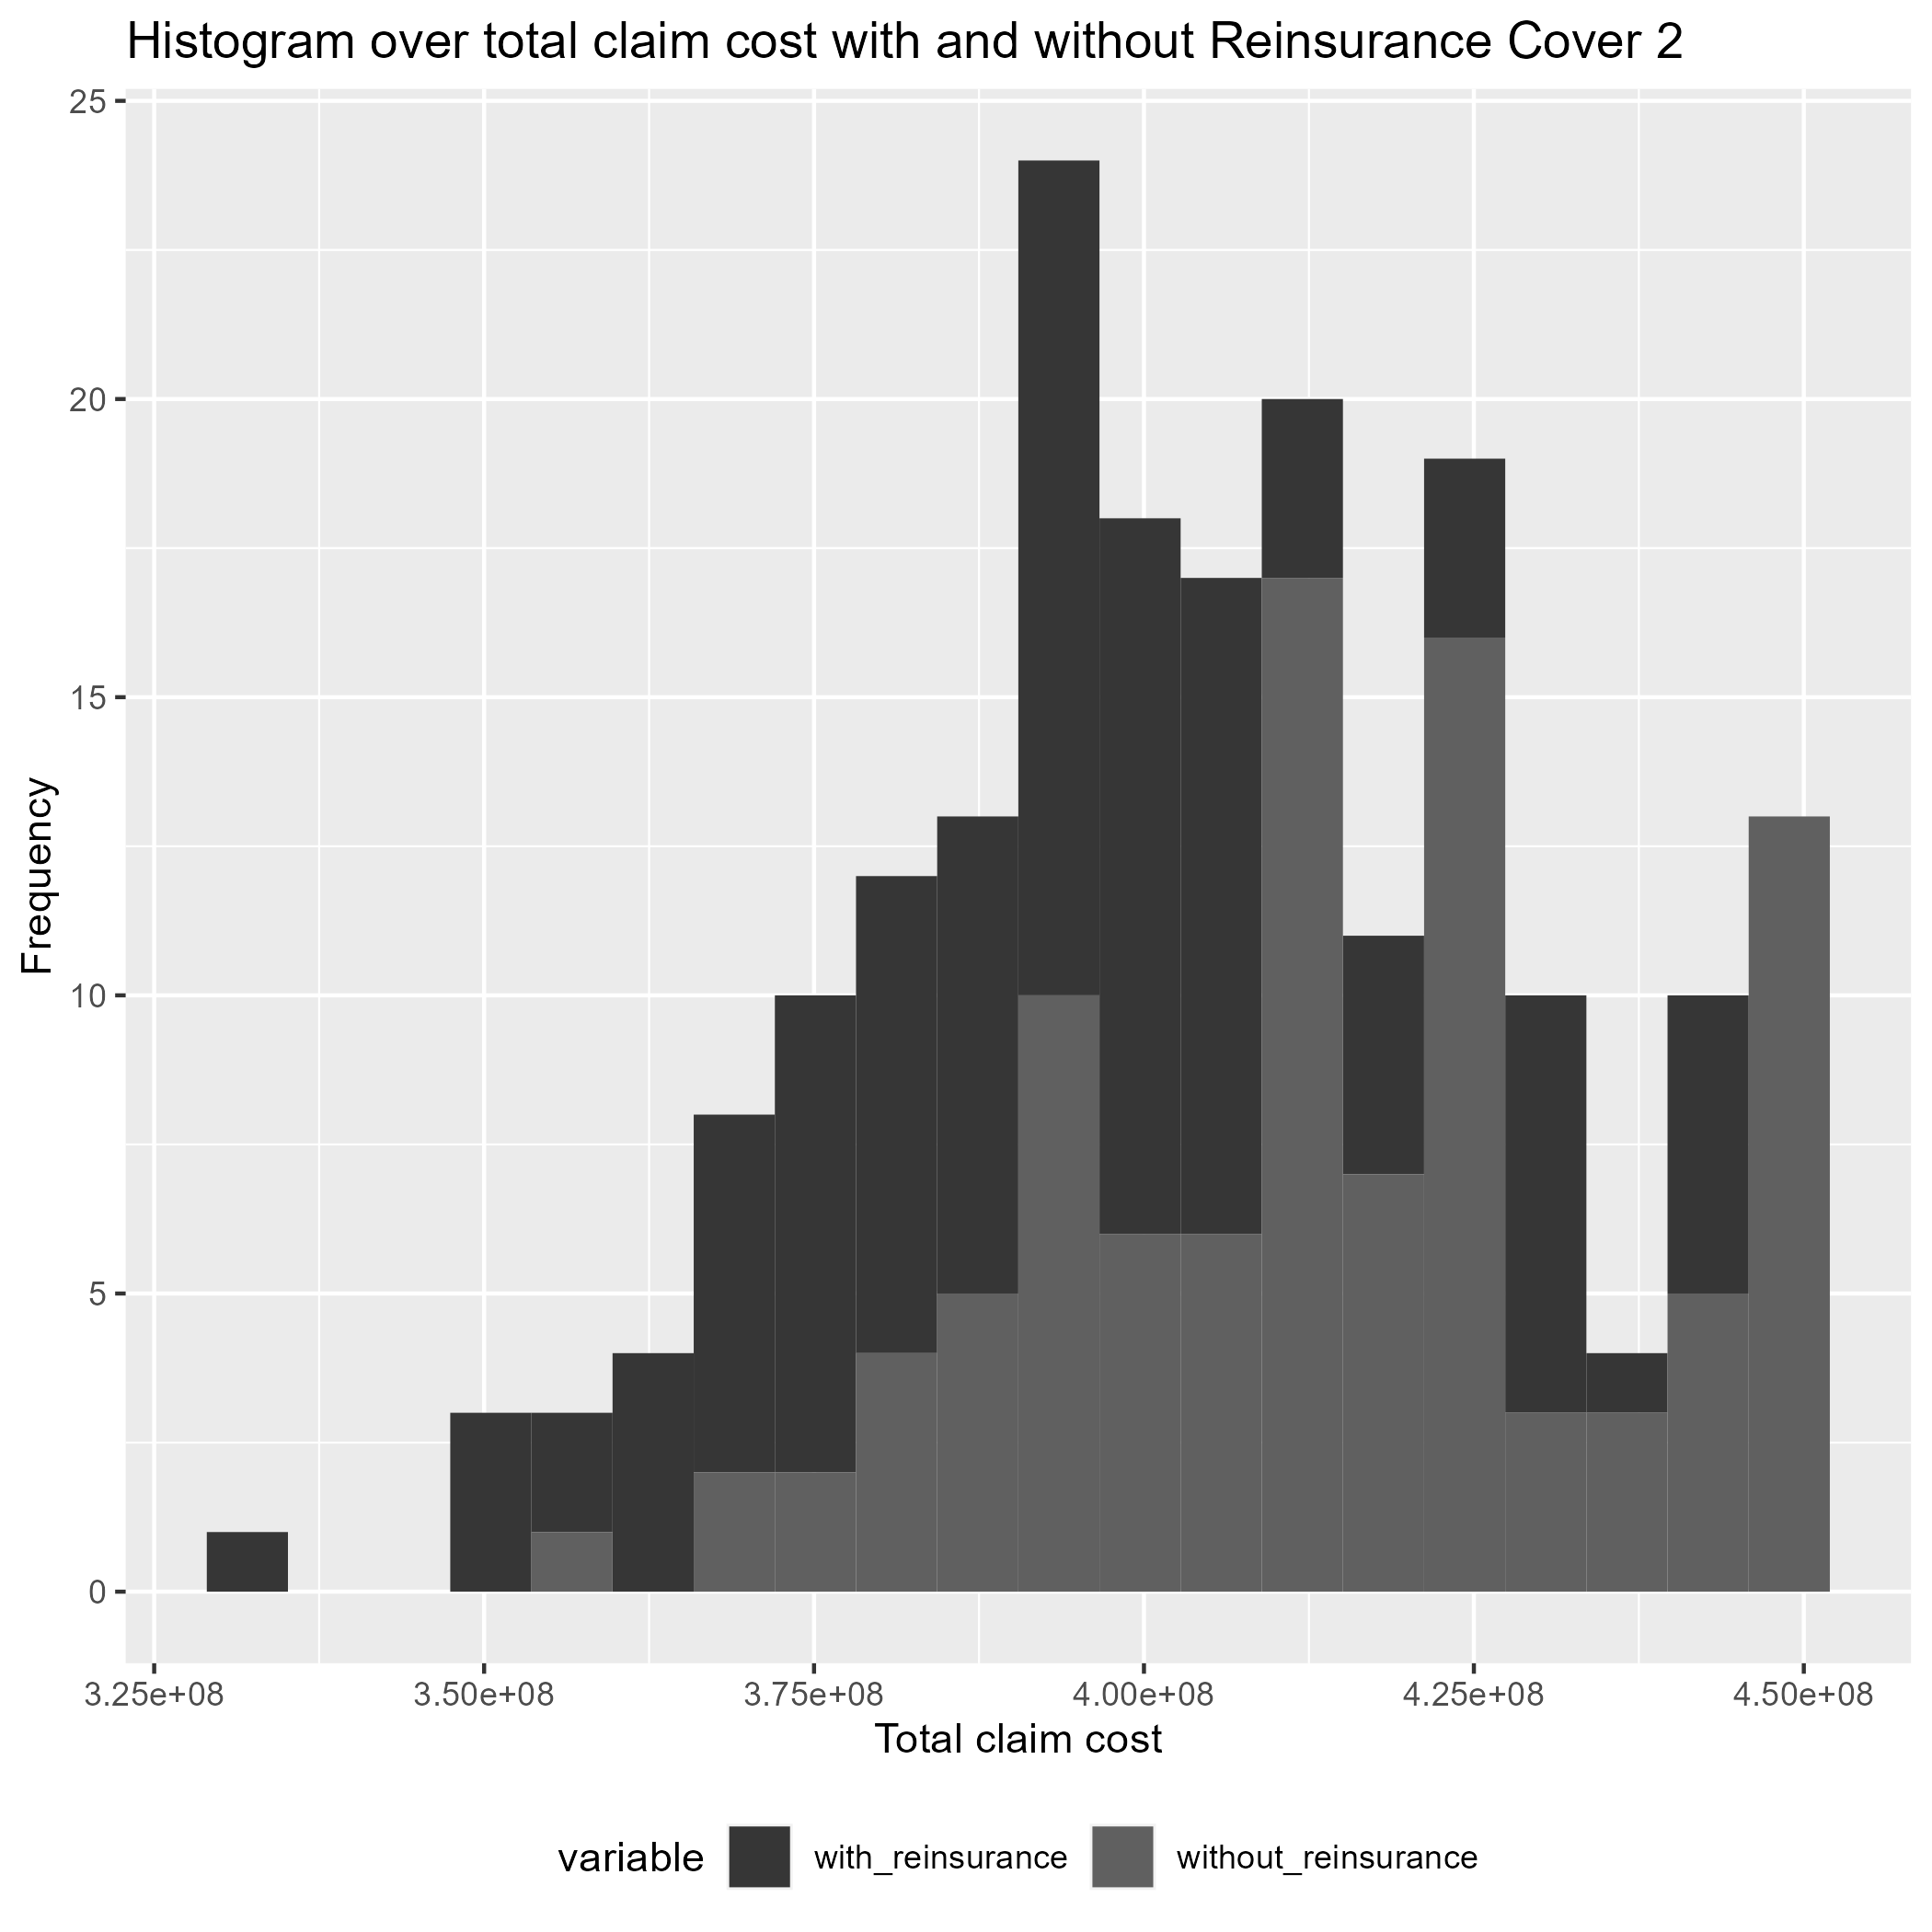
\includegraphics[width=.9\linewidth]{plots/reinsurance2/histogram_total_claim_cost_with_reinsurance.png}
      \caption{Distribution of total claim amounts.}
    \end{subfigure}
    \begin{subfigure}{.49\textwidth}
      \centering
      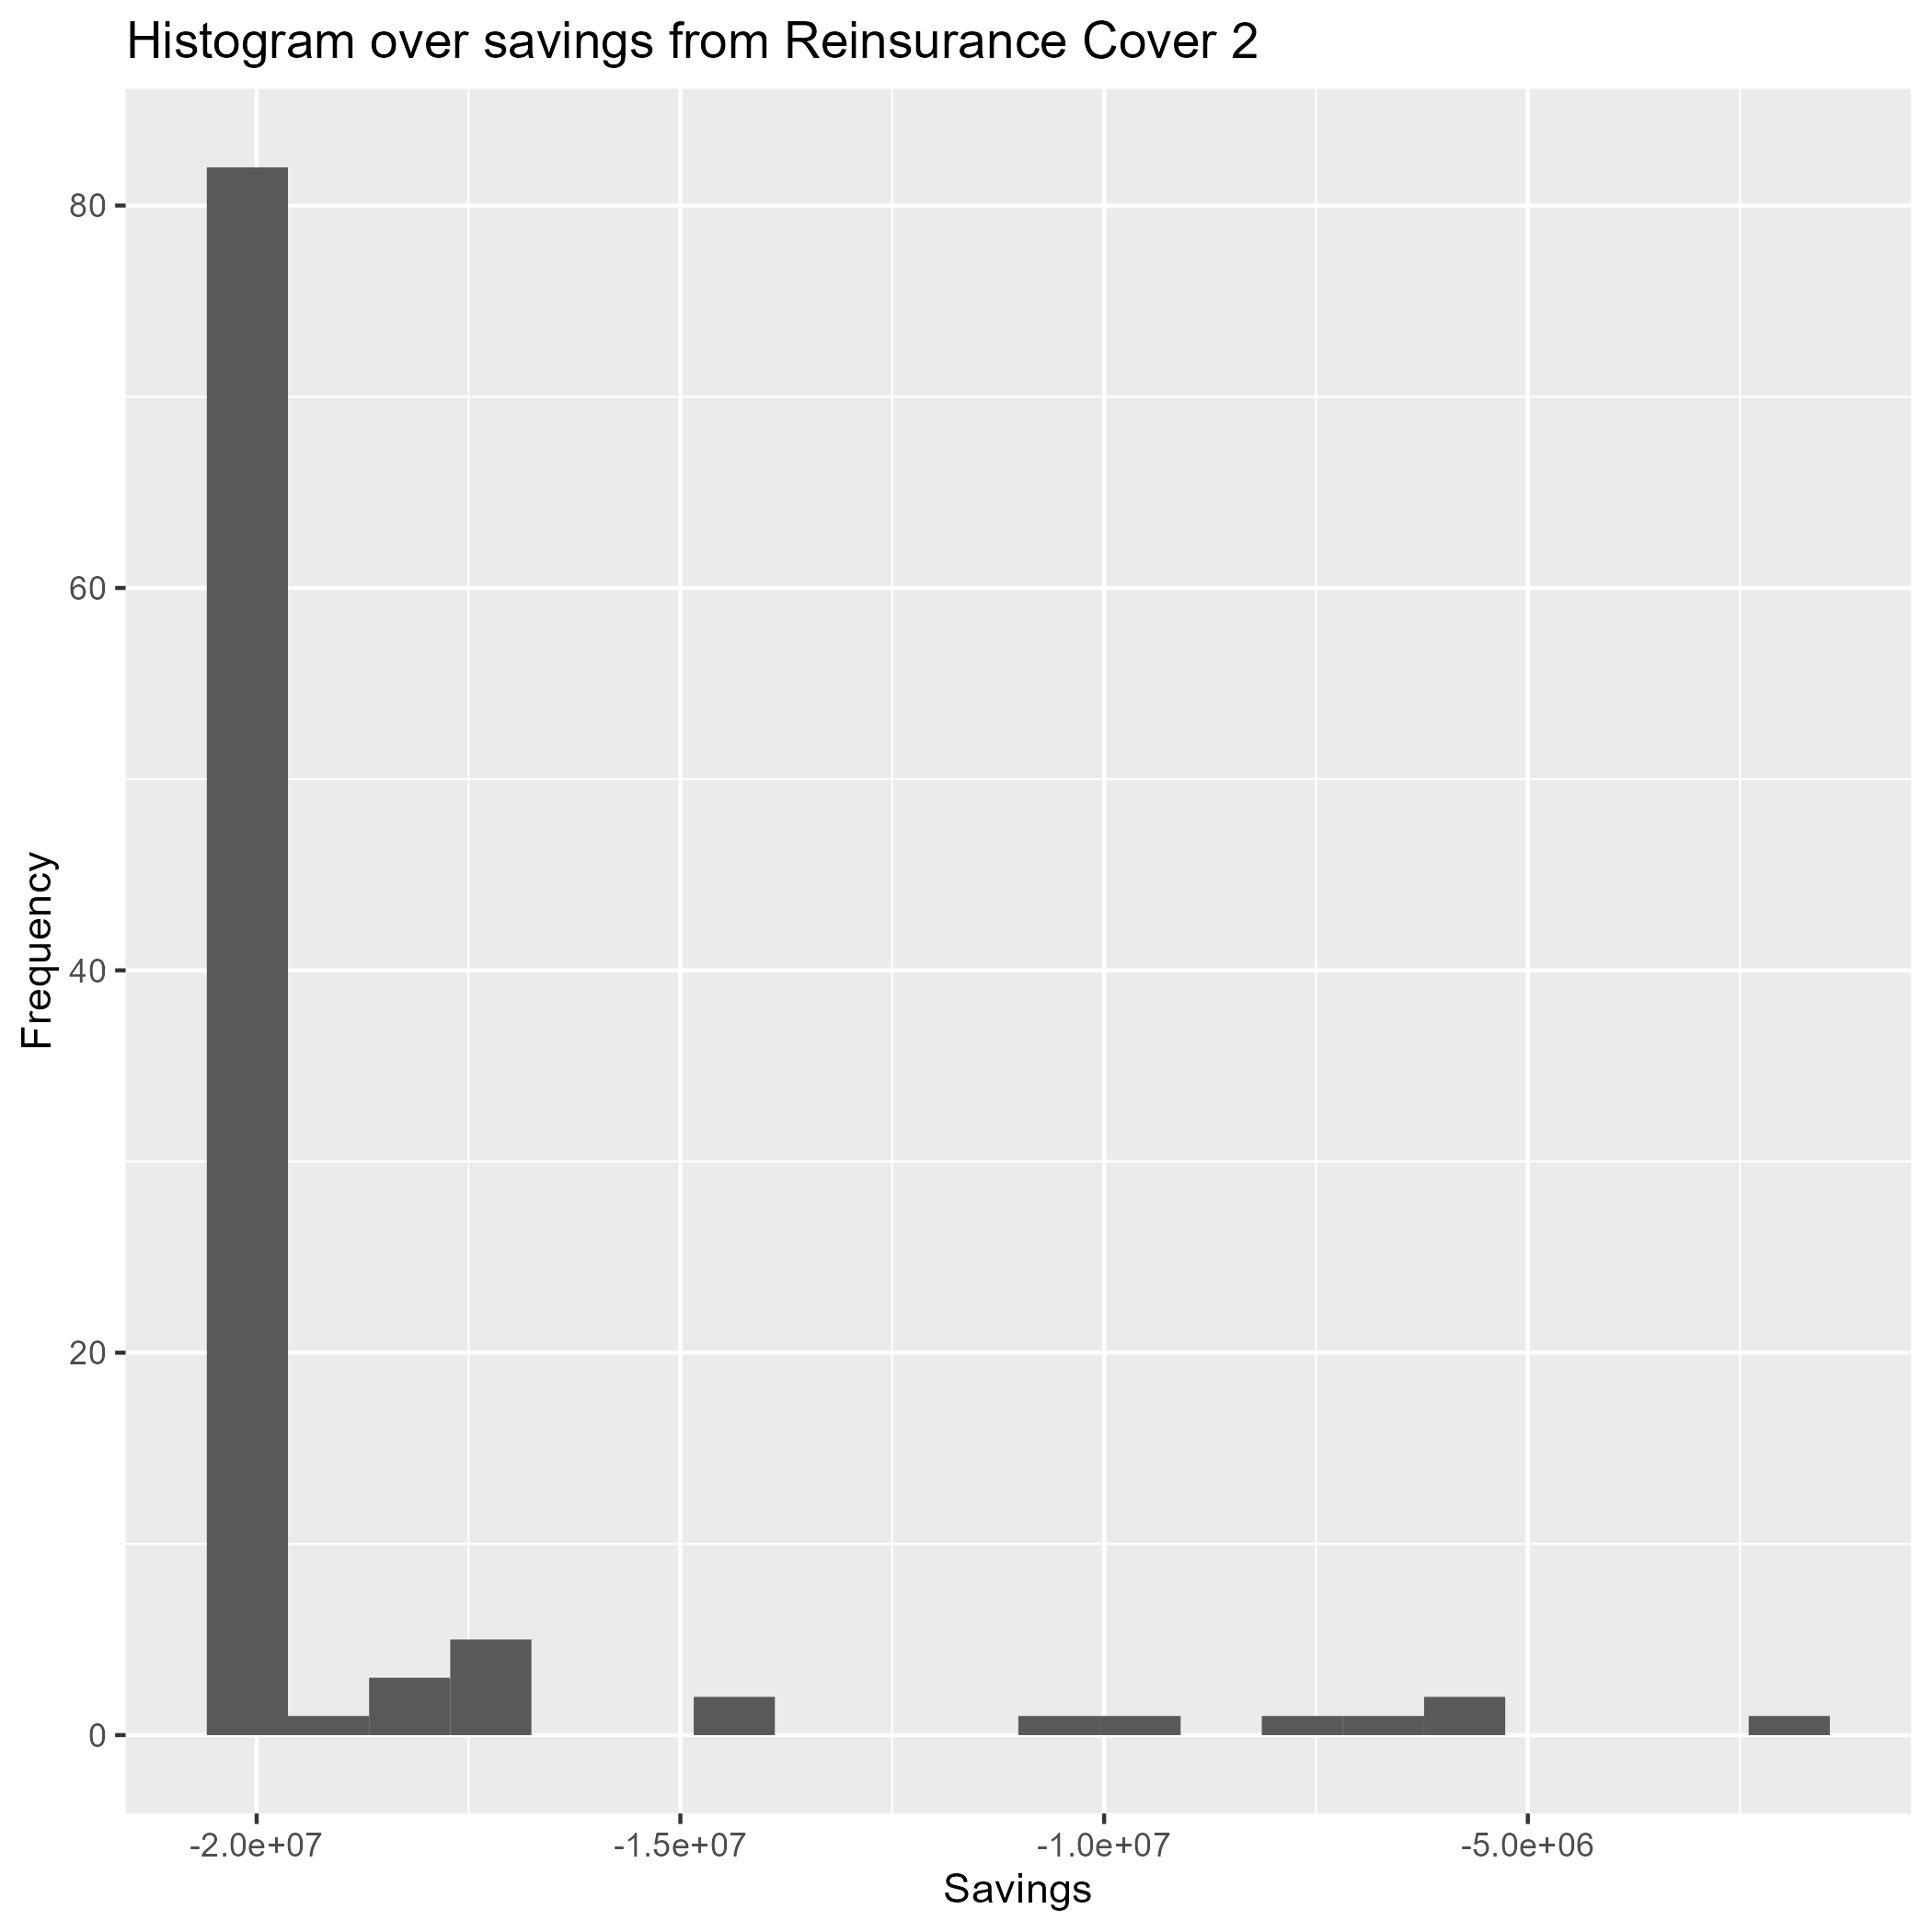
\includegraphics[width=.9\linewidth]{plots/reinsurance2/histogram_savings.png}
      \caption{Savings with Reinsurance.}
    \end{subfigure}
    \caption{Estimated quantiles and impact on a simulated claim distribution.}
    \label{a6:claim_cost}
\end{figure}

In the end, the stop-loss type cover may not be the most suitable for our claim process.
Mostly as we have such normality in our data that an extreme quantile event is near impossible on a portfolio level.
Instead the XL-covers may be more suitable due to large and small claim nature of both our insurance branches.


\subsubsection*{The SL Cover 2}
The final cover is the SL Cover across both branches, studying this we see in figure \ref{a7:claim_cost} very similar results to \ref{a6:claim_cost}.
Only in very rare circumstances do we get use of this reinsurance, and only then we even more rarely cover the excess premium reinsurance company is charging us.

Again, as stated the SL Cover 1, due to the normality in our claim process, and no sign of extreme events that would impact the portfolio level, there is little use of this SL-Cover.
In a real world scenario, with winters getting colder,   summer getting warmer and extreme events becoming more cover, this would be a consideration.
But as we currently see no signs of this in the data, there is little use of this in our cover.
But it could be an idea for next years assignment to add extreme portfolio level events that would occur every second year or similar.


 \begin{figure}[!h]
\centering
    \begin{subfigure}{.32\textwidth}
      \centering
      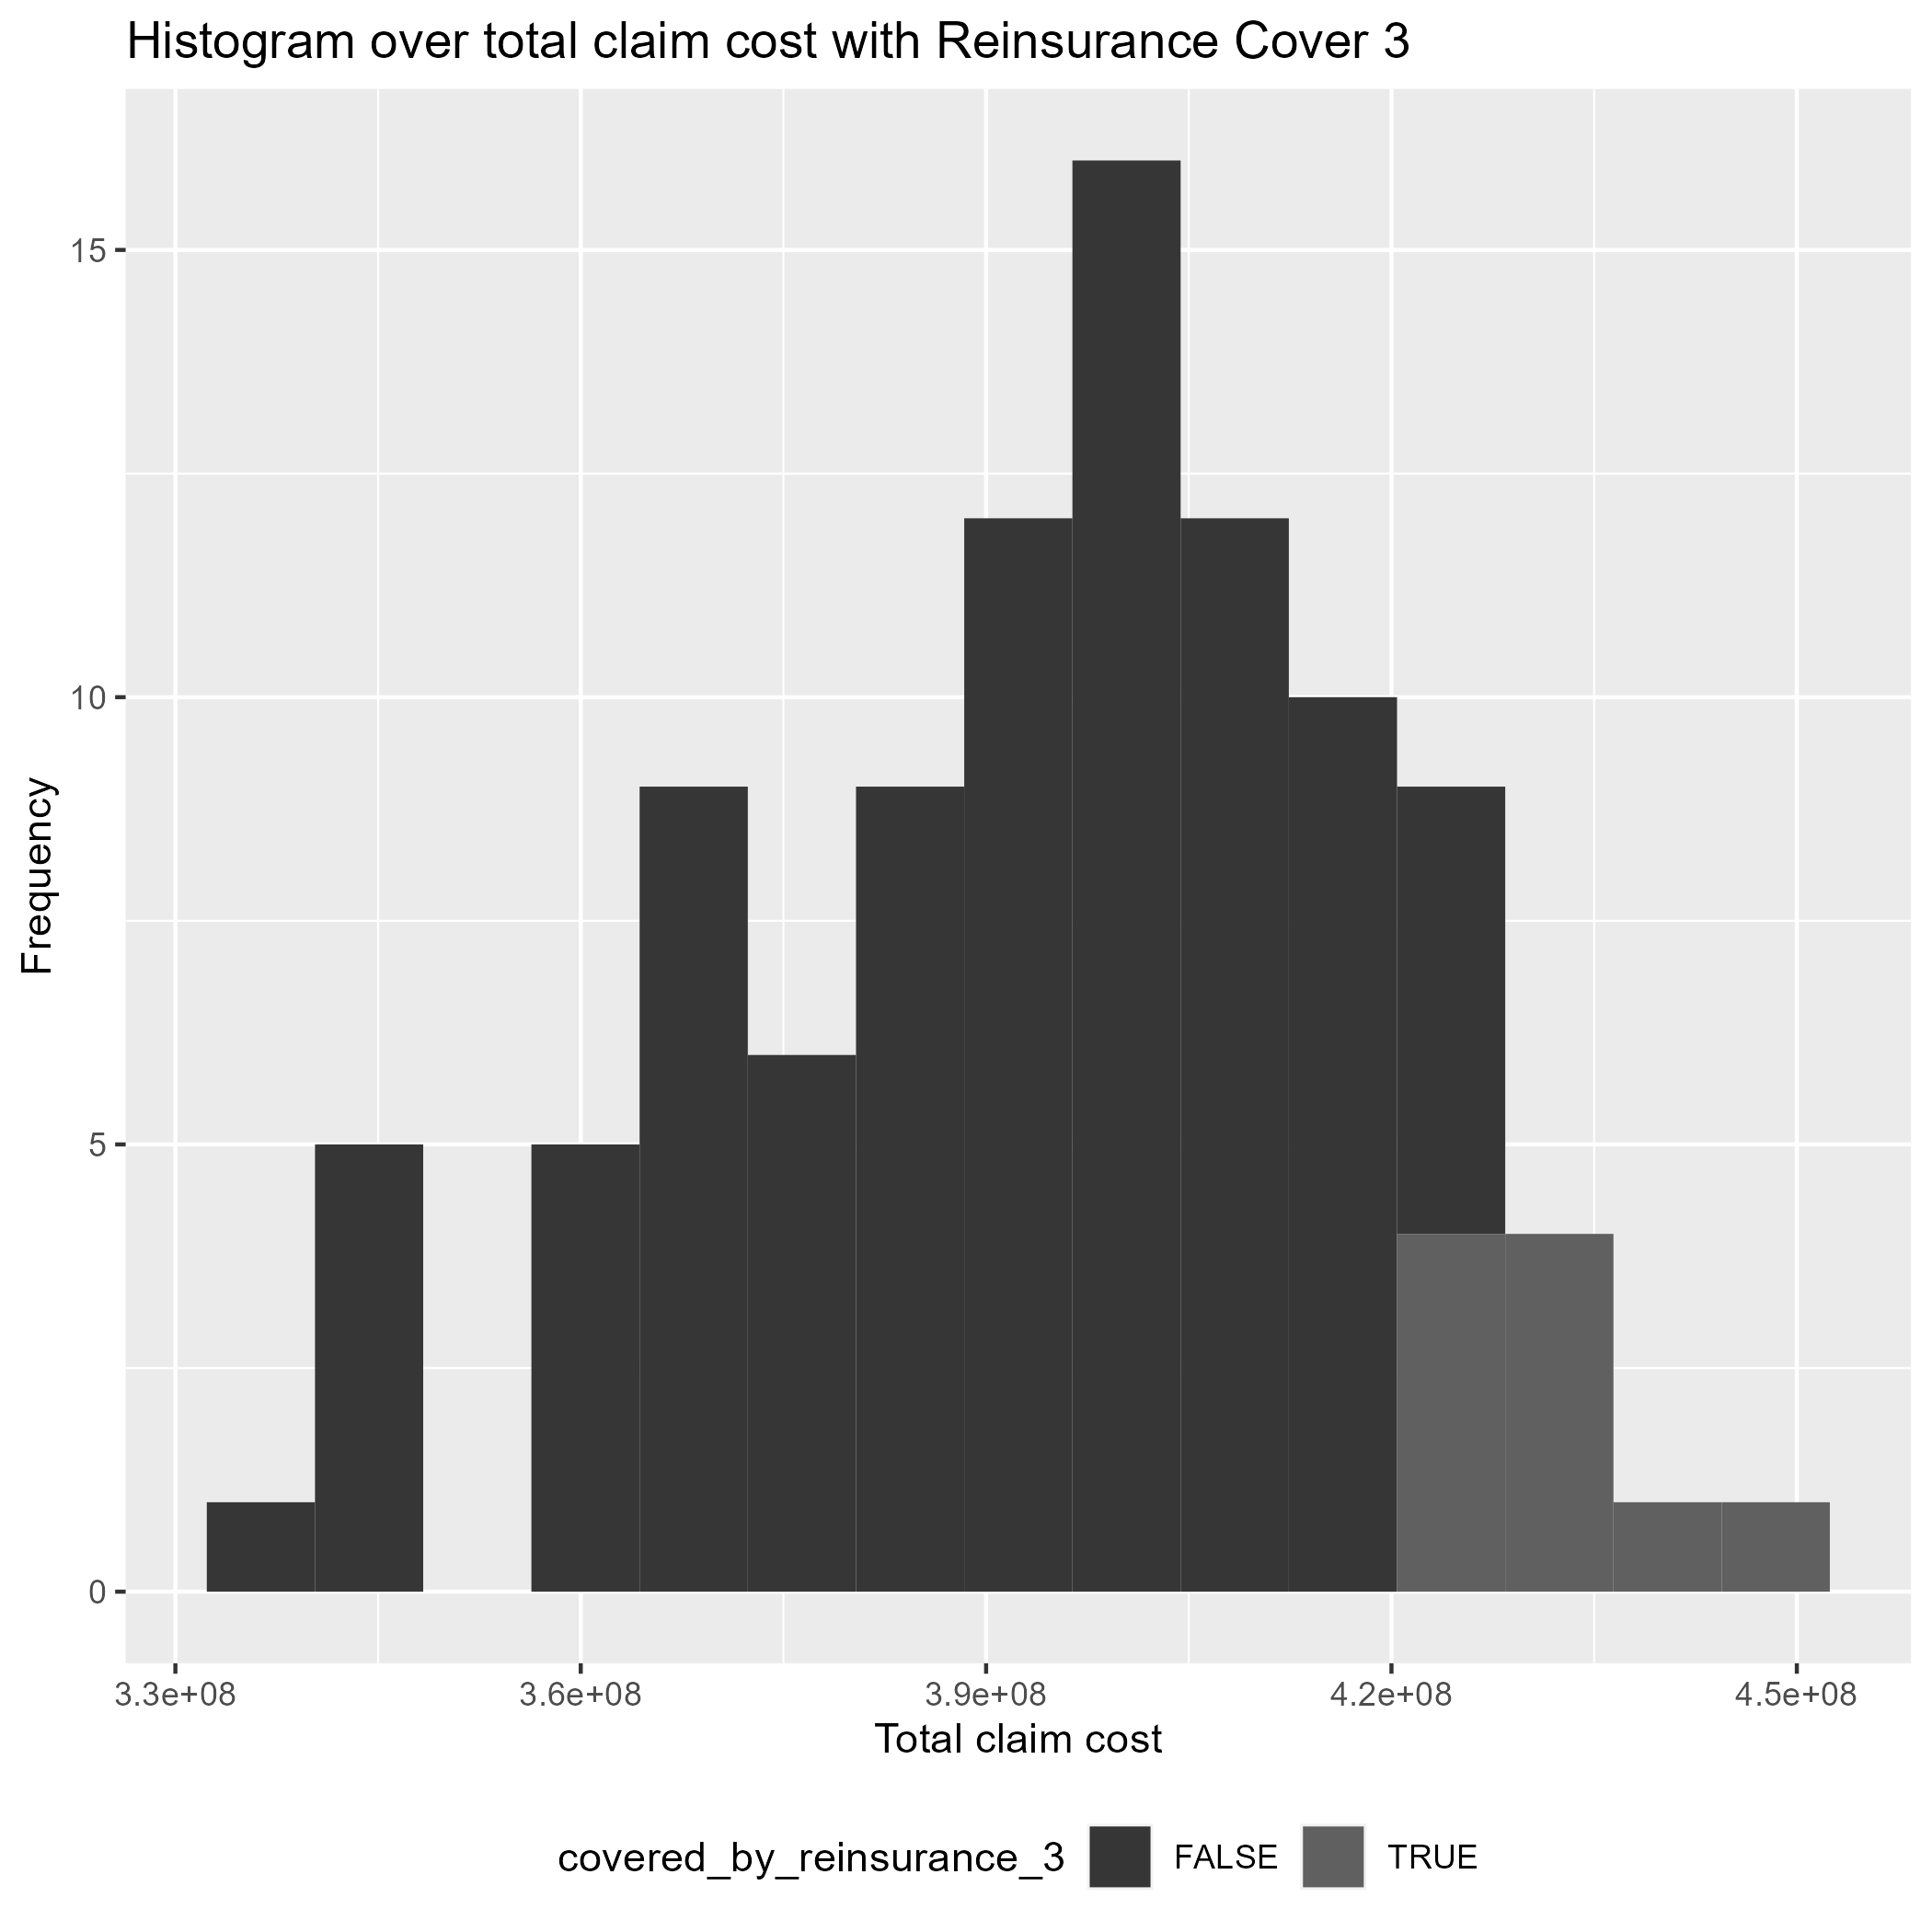
\includegraphics[width=.9\linewidth]{plots/reinsurance3/histogram_total_claim_cost_reinsurance3.png}
      \caption{Estimated quantiles.}
    \end{subfigure}
    \begin{subfigure}{.32\textwidth}
      \centering
      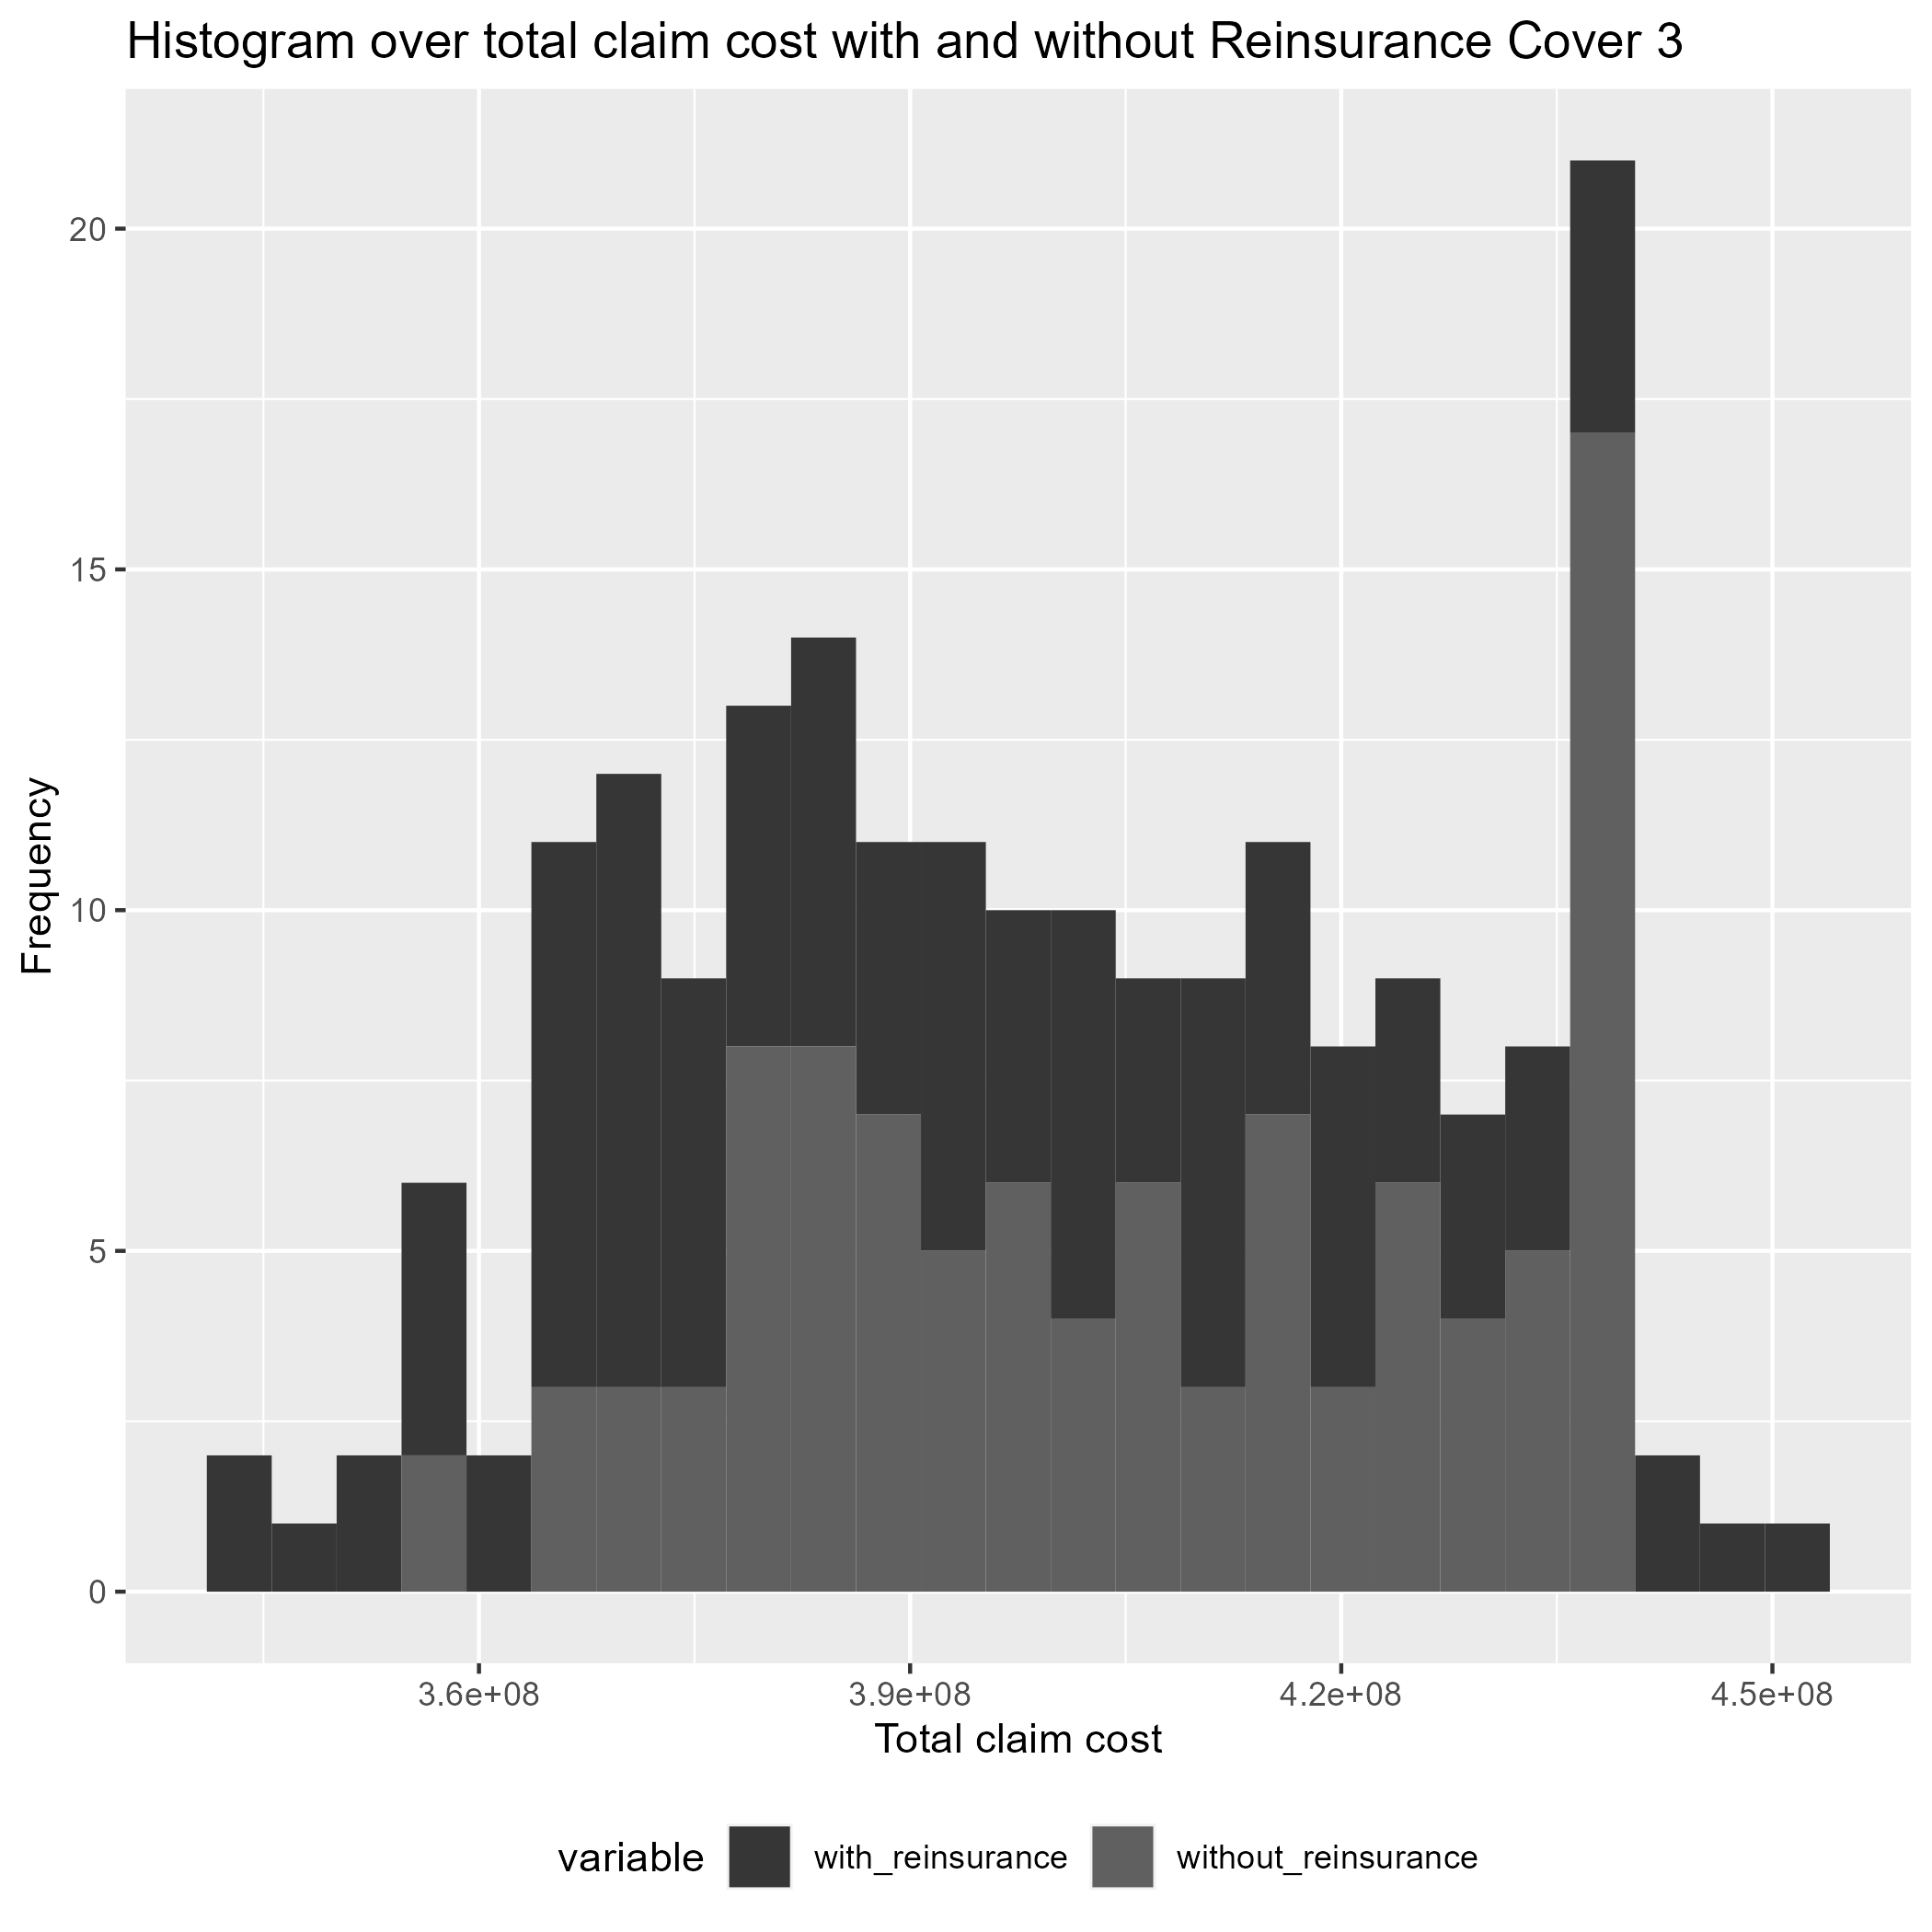
\includegraphics[width=.9\linewidth]{plots/reinsurance3/histogram_total_claim_cost_with_reinsurance.png}
      \caption{Total Claim Cost.}
    \end{subfigure}
    \begin{subfigure}{.32\textwidth}
      \centering
      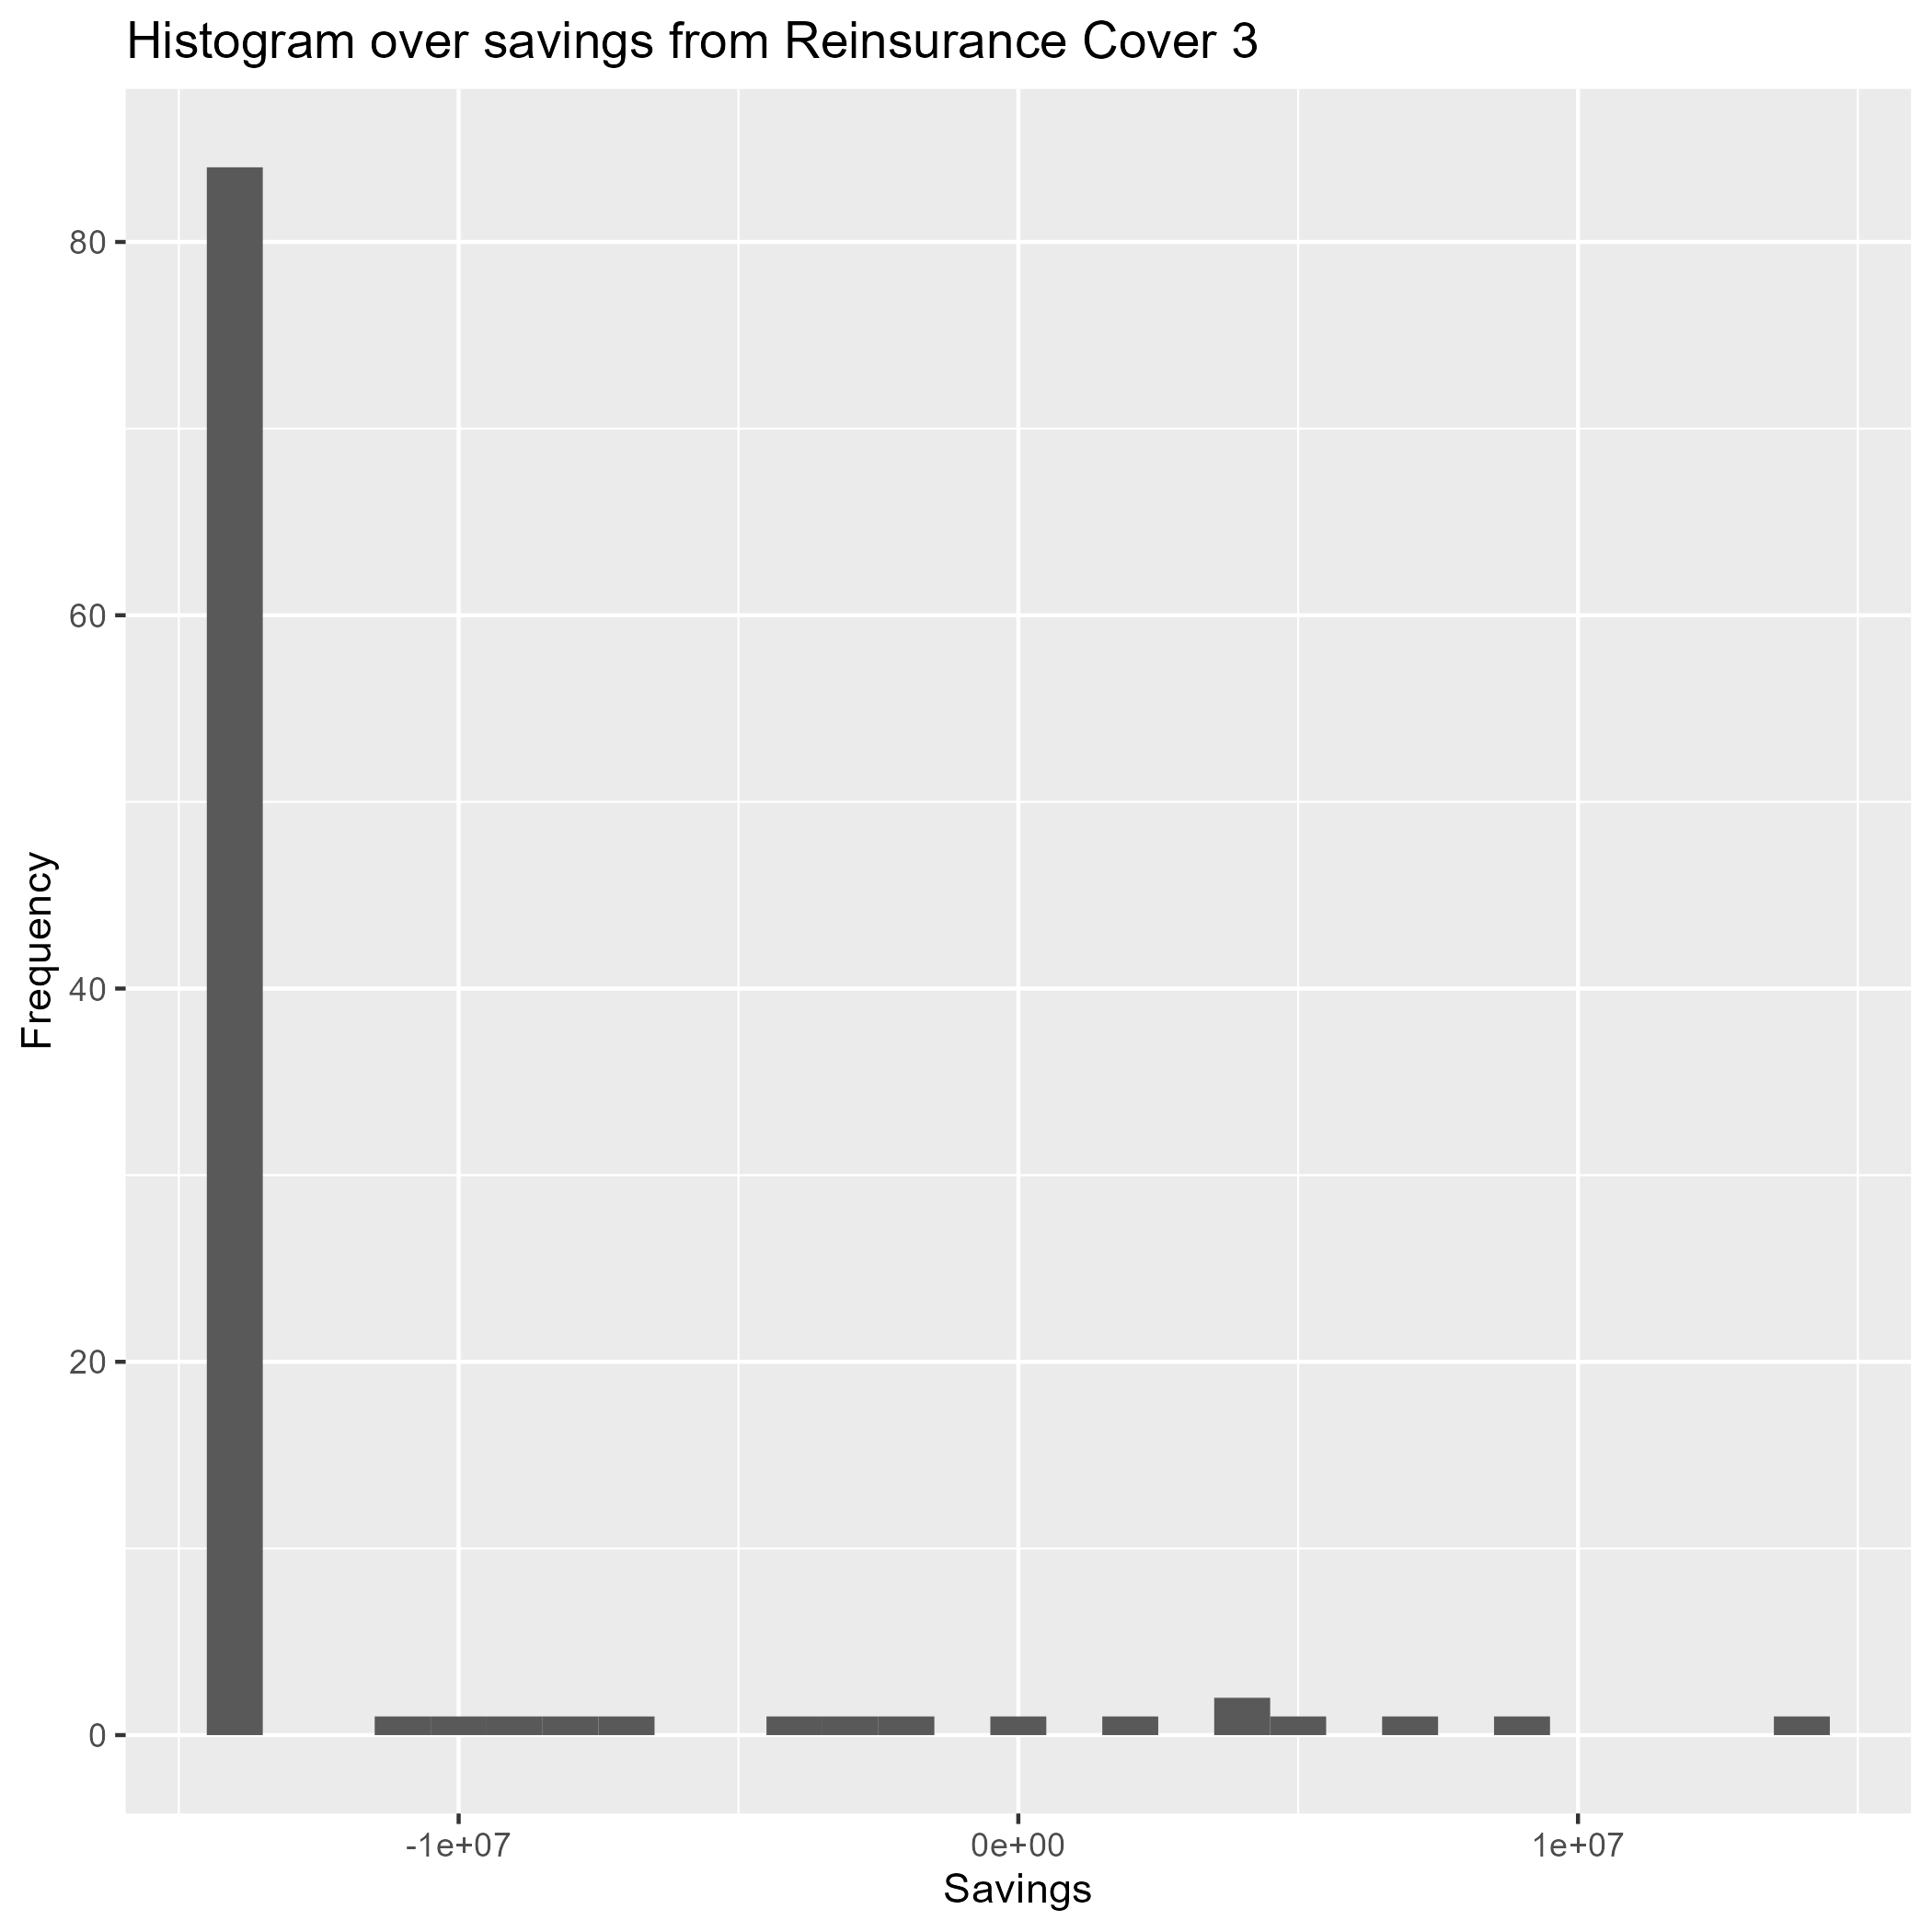
\includegraphics[width=.9\linewidth]{plots/reinsurance3/histogram_savings.png}
      \caption{Savings with Reinsurance.}
    \end{subfigure}
    \caption{Estimated quantiles and impact on a simulated claim distribution.}
    \label{a7:claim_cost}
\end{figure}

\subsection*{Conclusions}
We have in this assignment studied and simulated a portfolio of insurances belonging to 2 different branches.
What we have seen is that these 2 branches correlate and that there is a clear seasonal effect in claims.
We have also seen that the claim size can be divided in small and large and that these can be modeled seperately.
We have hypothised that the branches revolve along motor insurance, with branch 1 being motor damages and branch 2 being personal damages.

We have from this created a model of distributions we have used to simulate the claim arrival and cost process.
Using this we evaluated 3 types of reinsurance cover, one being an excess-loss cover and 2 being stop-loss covers.
Overall the reinsurance was rarely profitable, as to be expected but we saw that the excess loss cover would provide much more stable results for our portfolio, even if less profitable.
This because of the inherit large to small claims dynamic we have seen in the data.
The stop-loss covers was rarely profitable, even in the cases of being used, and would likely not be suitable for our portfolio if we do not expect some future extreme events or claim intensity not yet seen in the data.

In the end, one could experiment with these reinsurance overs and combine XL and SL on the seperate branches to fix the optimal risk profile.
It all depends on what risk-profile the insurance company wants and how much they would pay for that.
The XL cover would be more financially stable which is practical if we have investors or other stakeholders to take into consideration.
The SL cover would be suitable if we expect changes not yet seen in the data, like extreme events which would cause larger intensity and claim size.
If we want to maximize profits and take more risk we should avoid the reinsurance.

% \newpage
% \section*{Code}

% \lstinputlisting[language=R, firstline=6]{code.r}


\end{document}  
